% !TeX spellcheck = en_US
% !TeX encoding = UTF-8

\documentclass[aps, 10pt, a4paper]{article}
\usepackage{graphics, graphicx}
\usepackage{fancyvrb, enumerate}
\usepackage{amsmath, amssymb, amscd, amsfonts}
\usepackage{geometry}
\usepackage{multirow}
\usepackage{url}
\usepackage{tikz}
\usepackage{listings, listing}
\usepackage{color}

\usetikzlibrary{shapes, arrows, calc, positioning}
\definecolor{codegreen}{rgb}{0, 0.6, 0}
\definecolor{codegray}{rgb}{0.5, 0.5, 0.5}
\definecolor{codepurple}{rgb}{0.58, 0, 0.82}
\definecolor{backcolour}{rgb}{0.95, 0.95, 0.92}
\lstdefinestyle{mystyle}
{
    backgroundcolor=\color{backcolour},   
    commentstyle=\color{codegreen},
    keywordstyle=\color{magenta},
    numberstyle=\tiny\color{codegray},
    stringstyle=\color{codepurple},
    basicstyle=\footnotesize,
    breakatwhitespace=false,         
    breaklines=true,                 
    captionpos=b,                    
    keepspaces=true,                 
    numbers=left,                    
    numbersep=5pt,                  
    showspaces=false,                
    showstringspaces=false,
    showtabs=false,                  
    tabsize=2,
    frame=single
}
\lstset{style=mystyle}
\tikzstyle{decision} = [diamond, draw, fill=blue!20, text width=4.5em, text badly centered, node distance=3cm, inner sep=0pt]
\tikzstyle{block} = [rectangle, draw, fill=blue!20, text width=5em, text centered, rounded corners, minimum height=2em]
\tikzstyle{line} = [draw, -latex']
\tikzstyle{cloud} = [draw, ellipse, fill=red!20, node distance=5em, minimum height=2em]
\tikzset
{
    -|-/.style=
    {
        to path=
        {
            (\tikztostart) -| ($(\tikztostart)!#1!(\tikztotarget)$) |- (\tikztotarget)
            \tikztonodes
        }
    },
    -|-/.default=0.5,
    |-|/.style=
    {
        to path=
        {
            (\tikztostart) |- ($(\tikztostart)!#1!(\tikztotarget)$) -| (\tikztotarget)
            \tikztonodes
        }
    },
    |-|/.default=0.5,
}
\geometry
{
    top = 20mm,
    bottom = 20mm,
    left = 20mm,
    right = 20mm
}

\title{Visualization Term Project}
\author{20141087 Ryeongyun Kim \and 20161206 Jaewoong Lee}
\date{\today}

\begin{document}
    \maketitle
    \newpage
    
    \tableofcontents
    \listoftables
    \listoffigures
    \newpage
    
    \section{Introduction}
        In this term project, we have to answer several question with virtual building data. 
    
    \section{Materials}
        \subsection{Building Layout}
            To analyzing movement data, we should find corresponding coordinate with zone data. To find matching coordinate, we calculate the approximate center of all zones, and consider the approximate center coordinate as representative of its zone. 
        
            \subsubsection{Main Layout}
                \begin{figure}[htbp]
                    \centering
                    $\begin{array}{ccc}
                        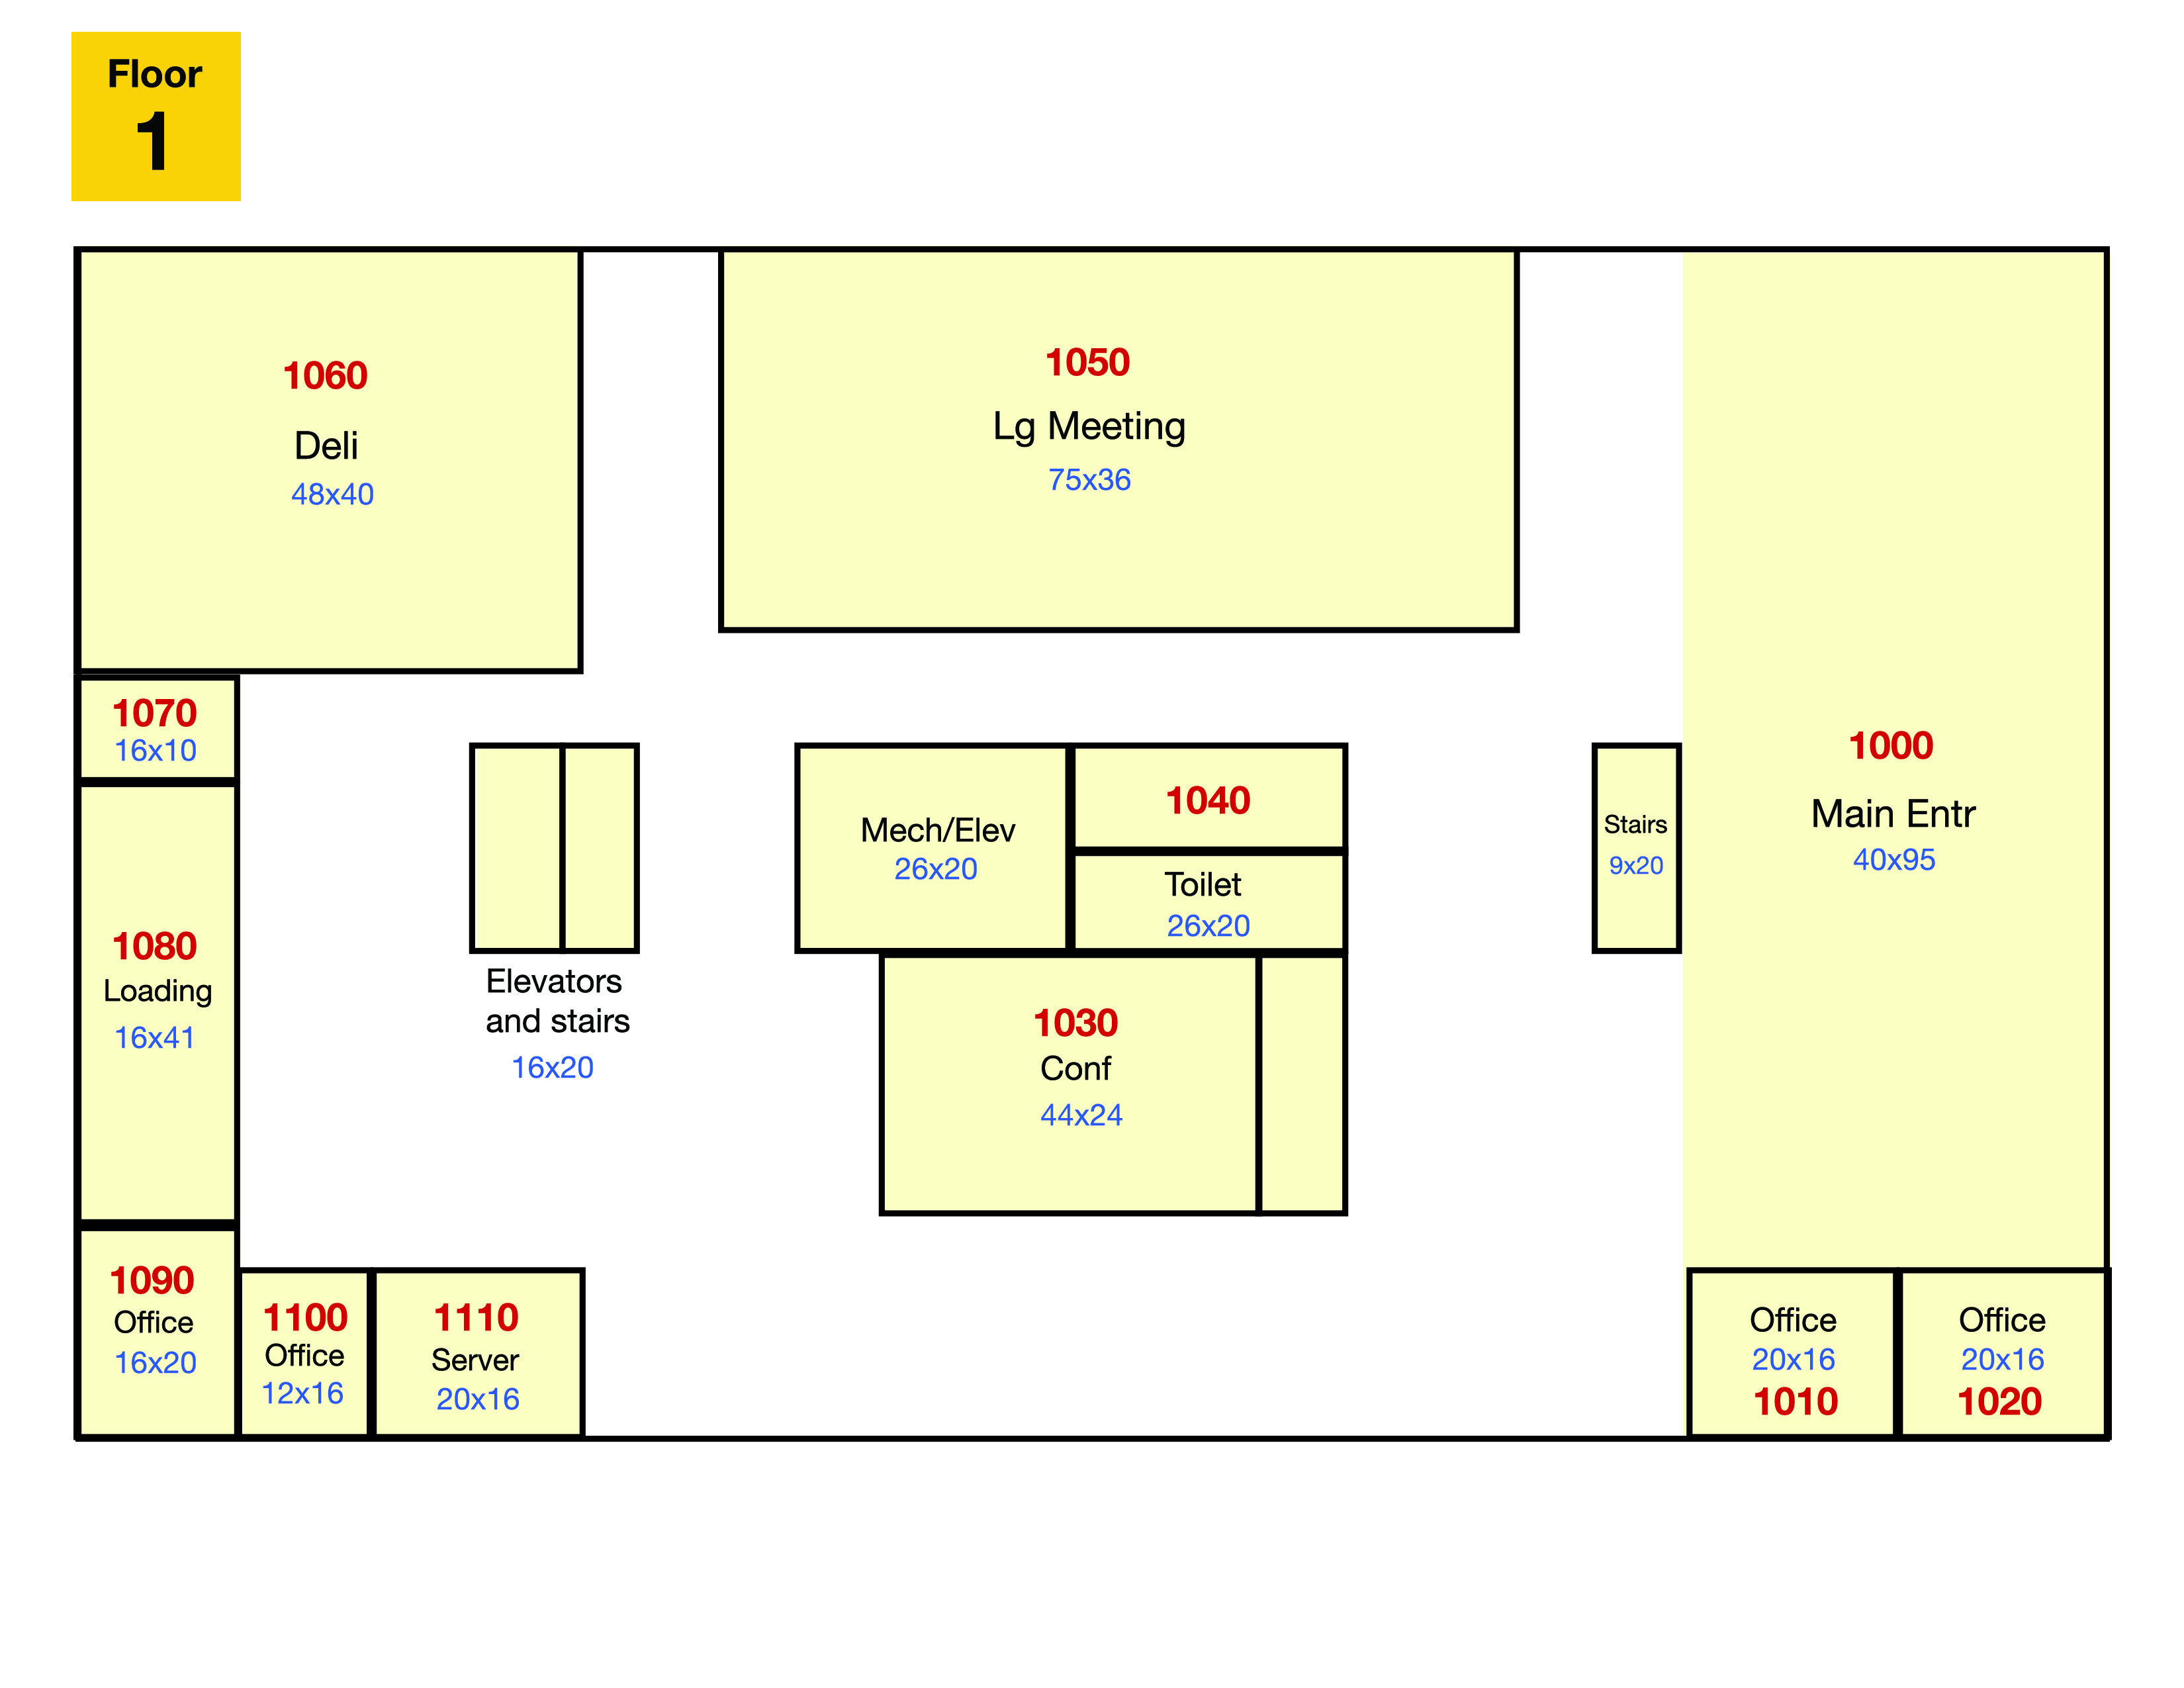
\includegraphics[width=0.3 \linewidth]{figures/basic1.jpg}
                        &
                        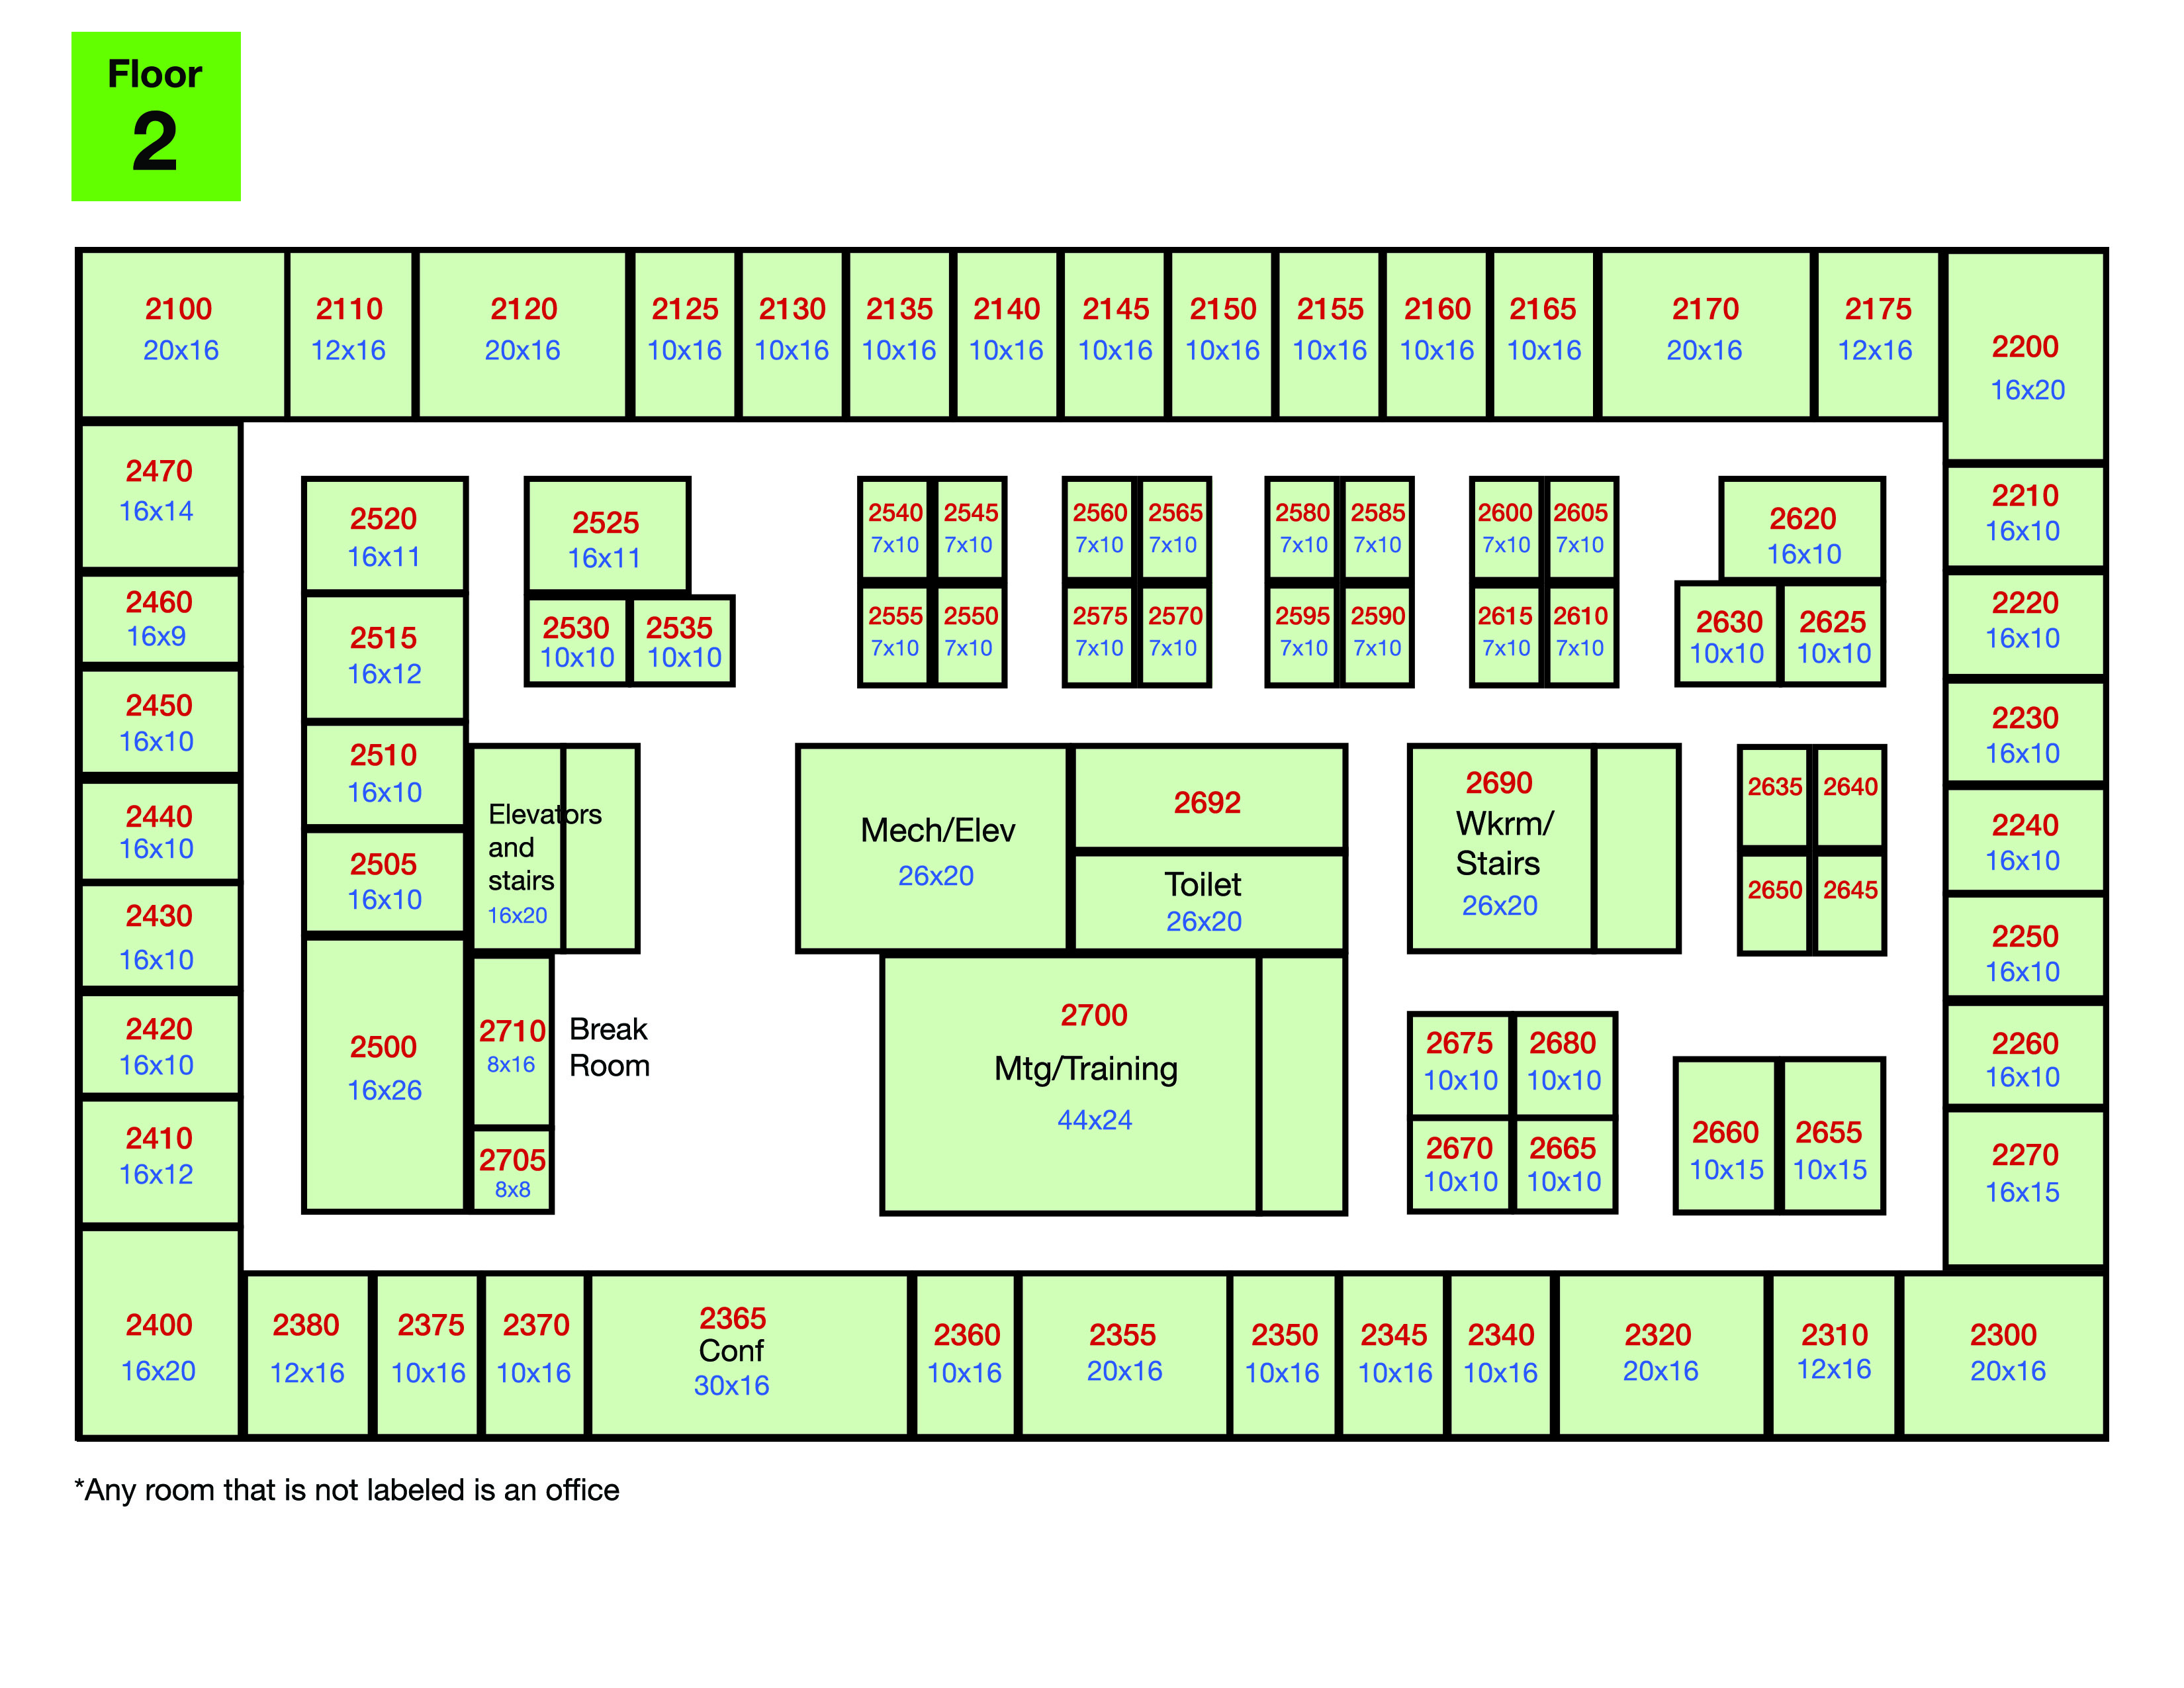
\includegraphics[width=0.3 \linewidth]{figures/basic2.jpg}
                        &
                        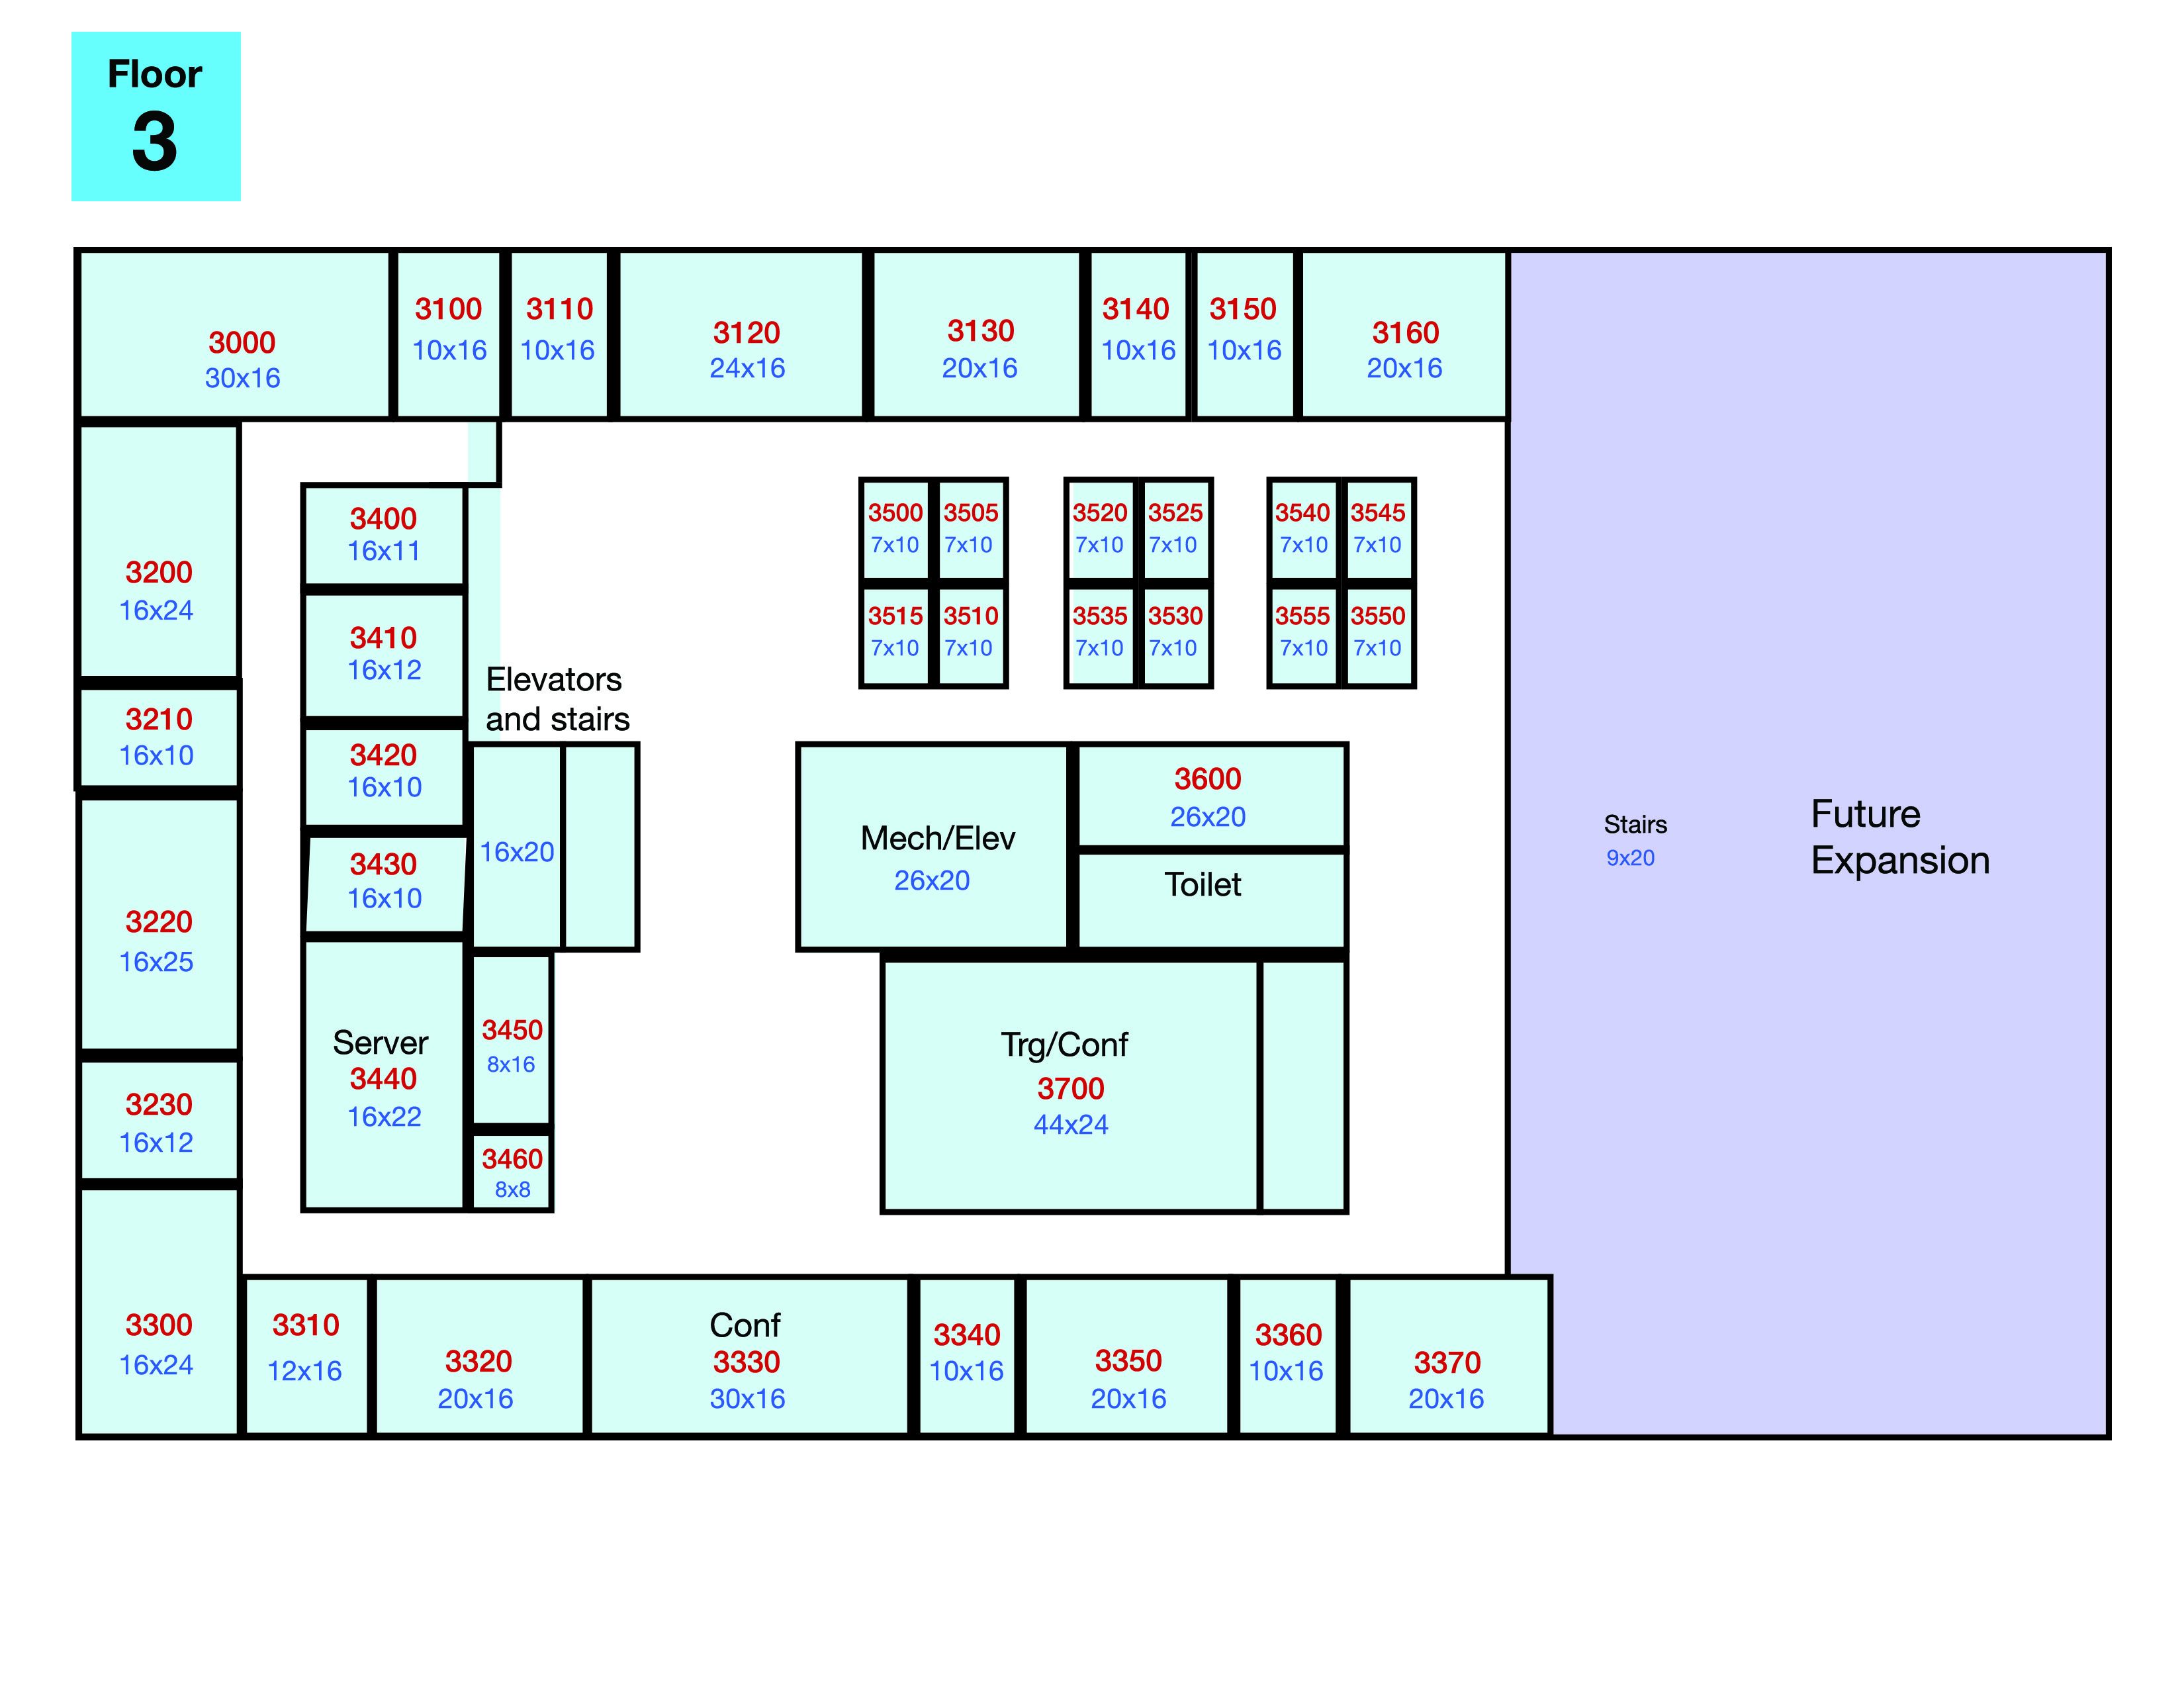
\includegraphics[width=0.3 \linewidth]{figures/basic3.jpg}
                        \\
                        
                        \mbox{(a) First Floor} & \mbox{(b) Second Floor} & \mbox{(c) Third Floor} \\
                    \end{array}$
                    \caption{Main Layout of the building}
                    \label{fig:main}
                \end{figure}
            
                The main layout of this building is as figure \ref{fig:main}. 
                
            \subsubsection{Energy Zone Layout}
                \begin{figure}[htbp]
                    \centering
                    $\begin{array}{ccc}
                        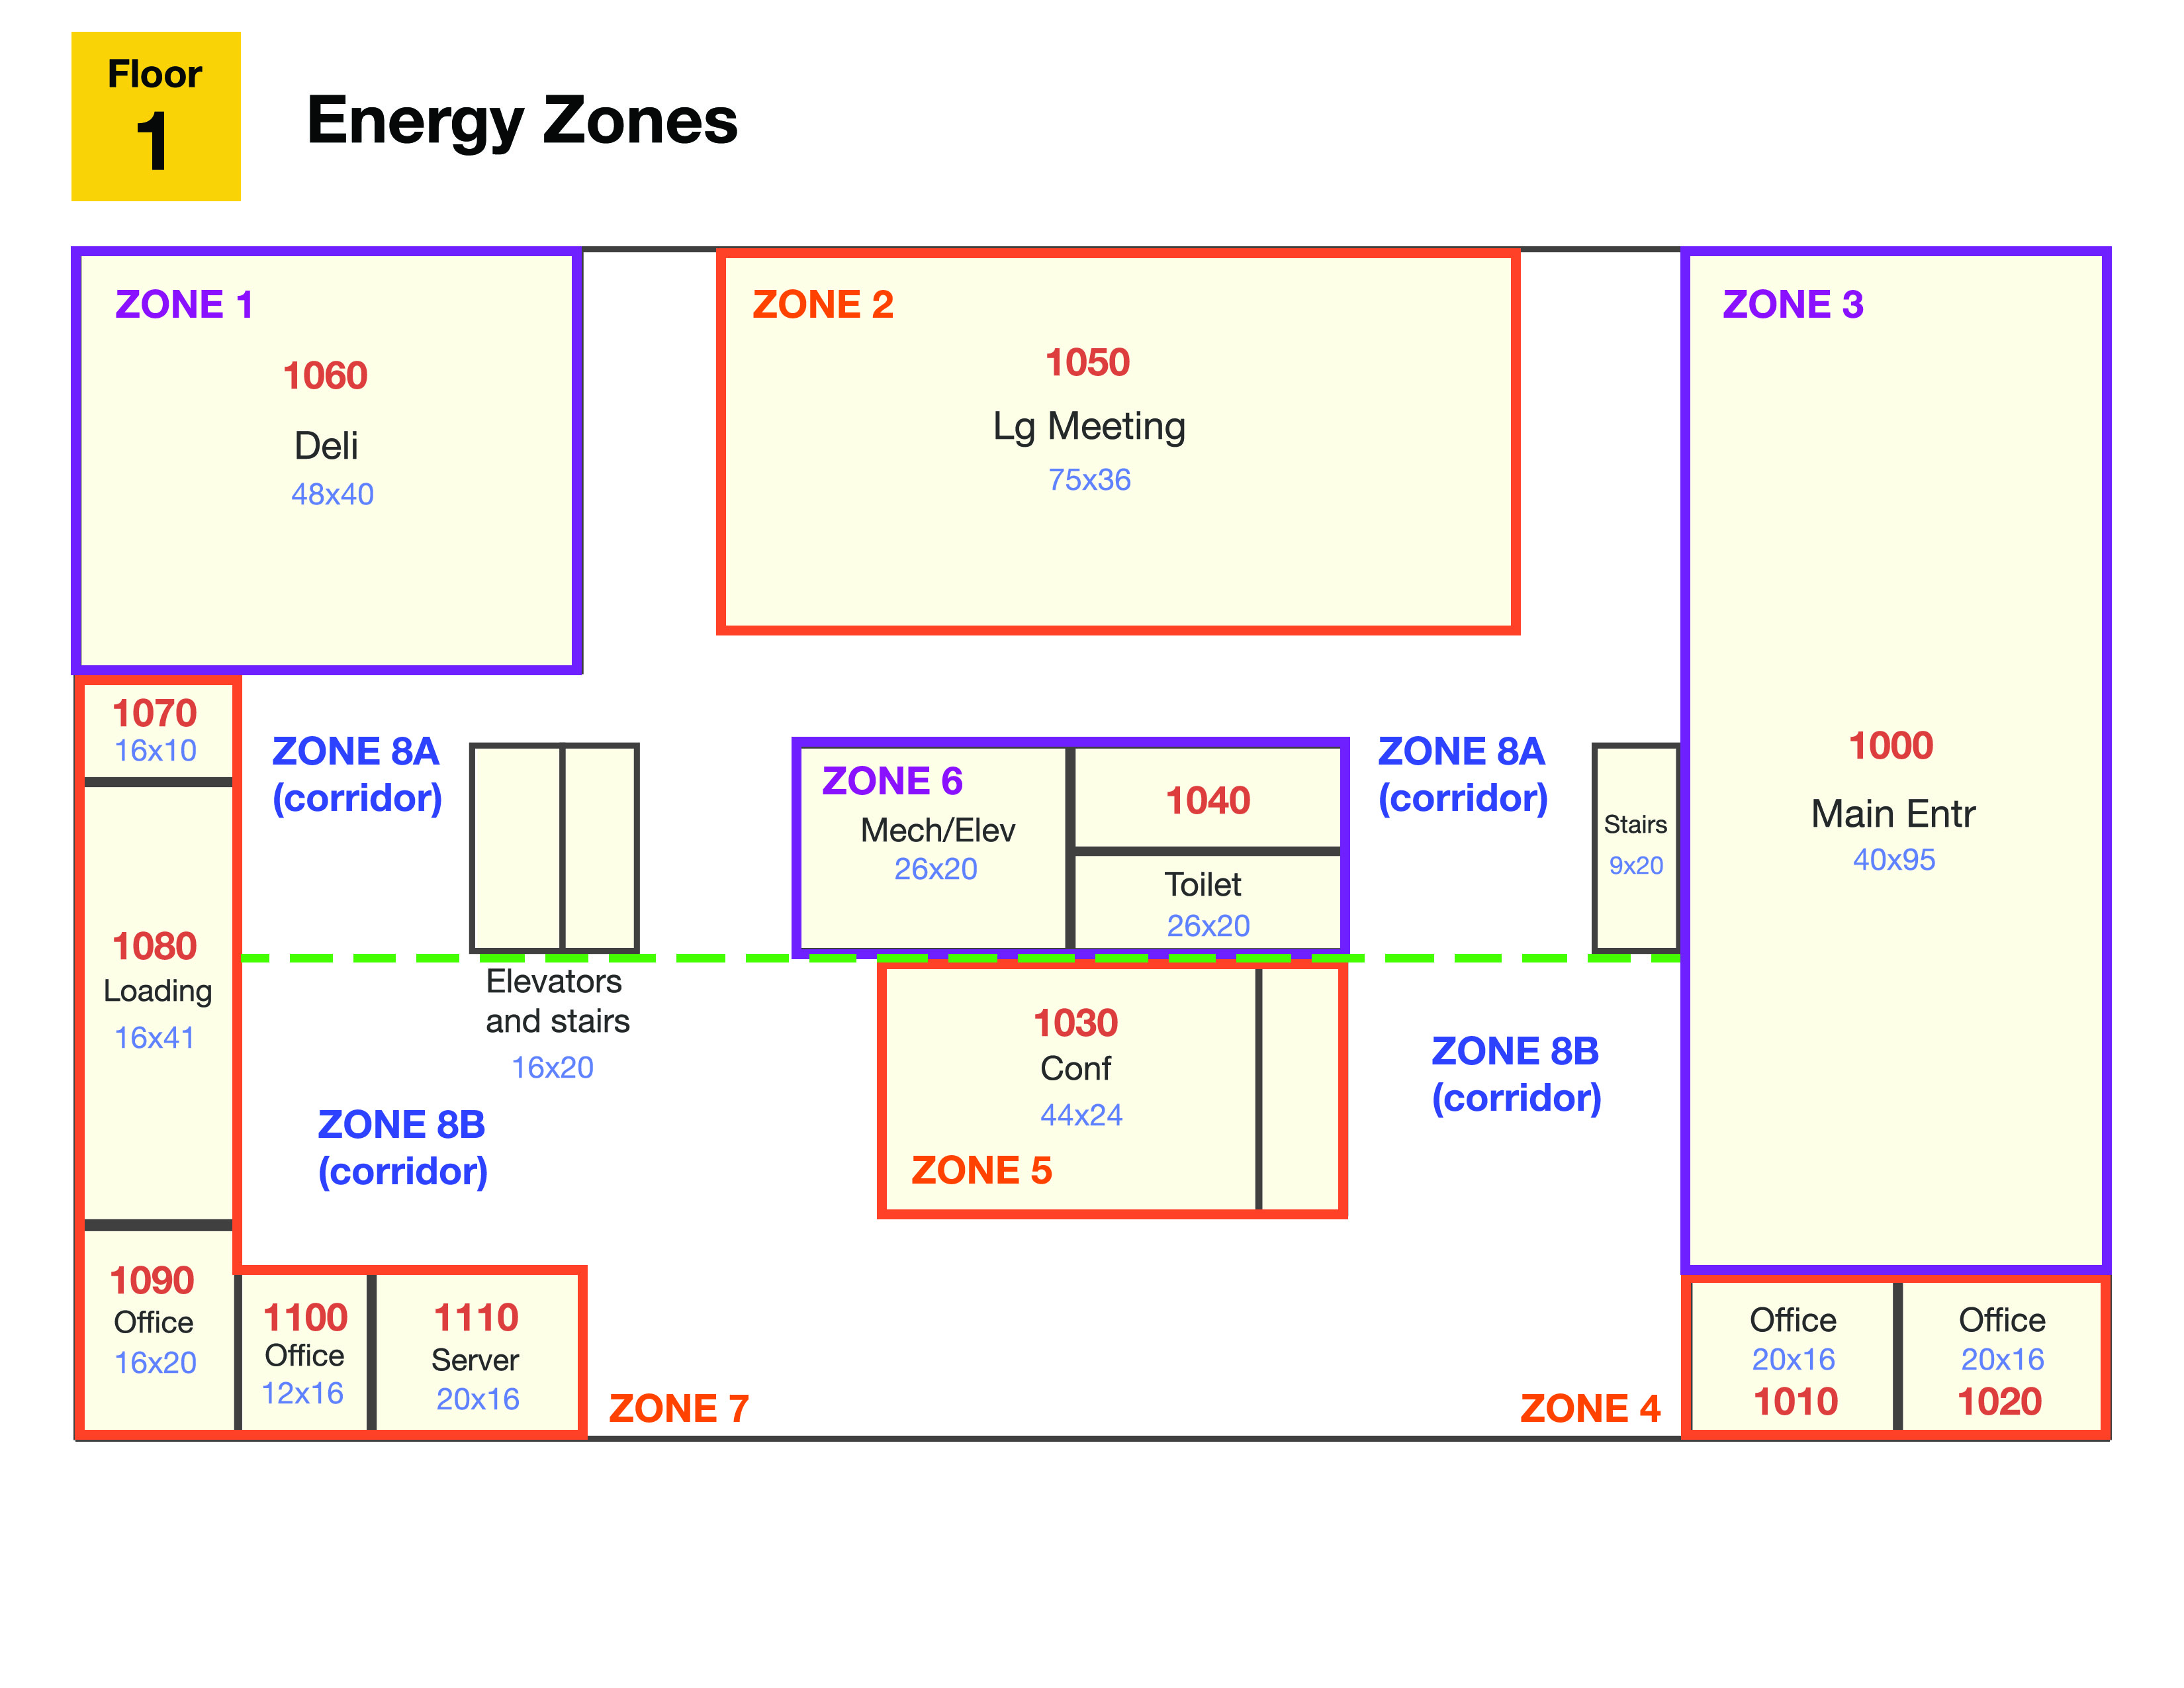
\includegraphics[width=0.3 \linewidth]{figures/energy1.jpg}
                        &
                        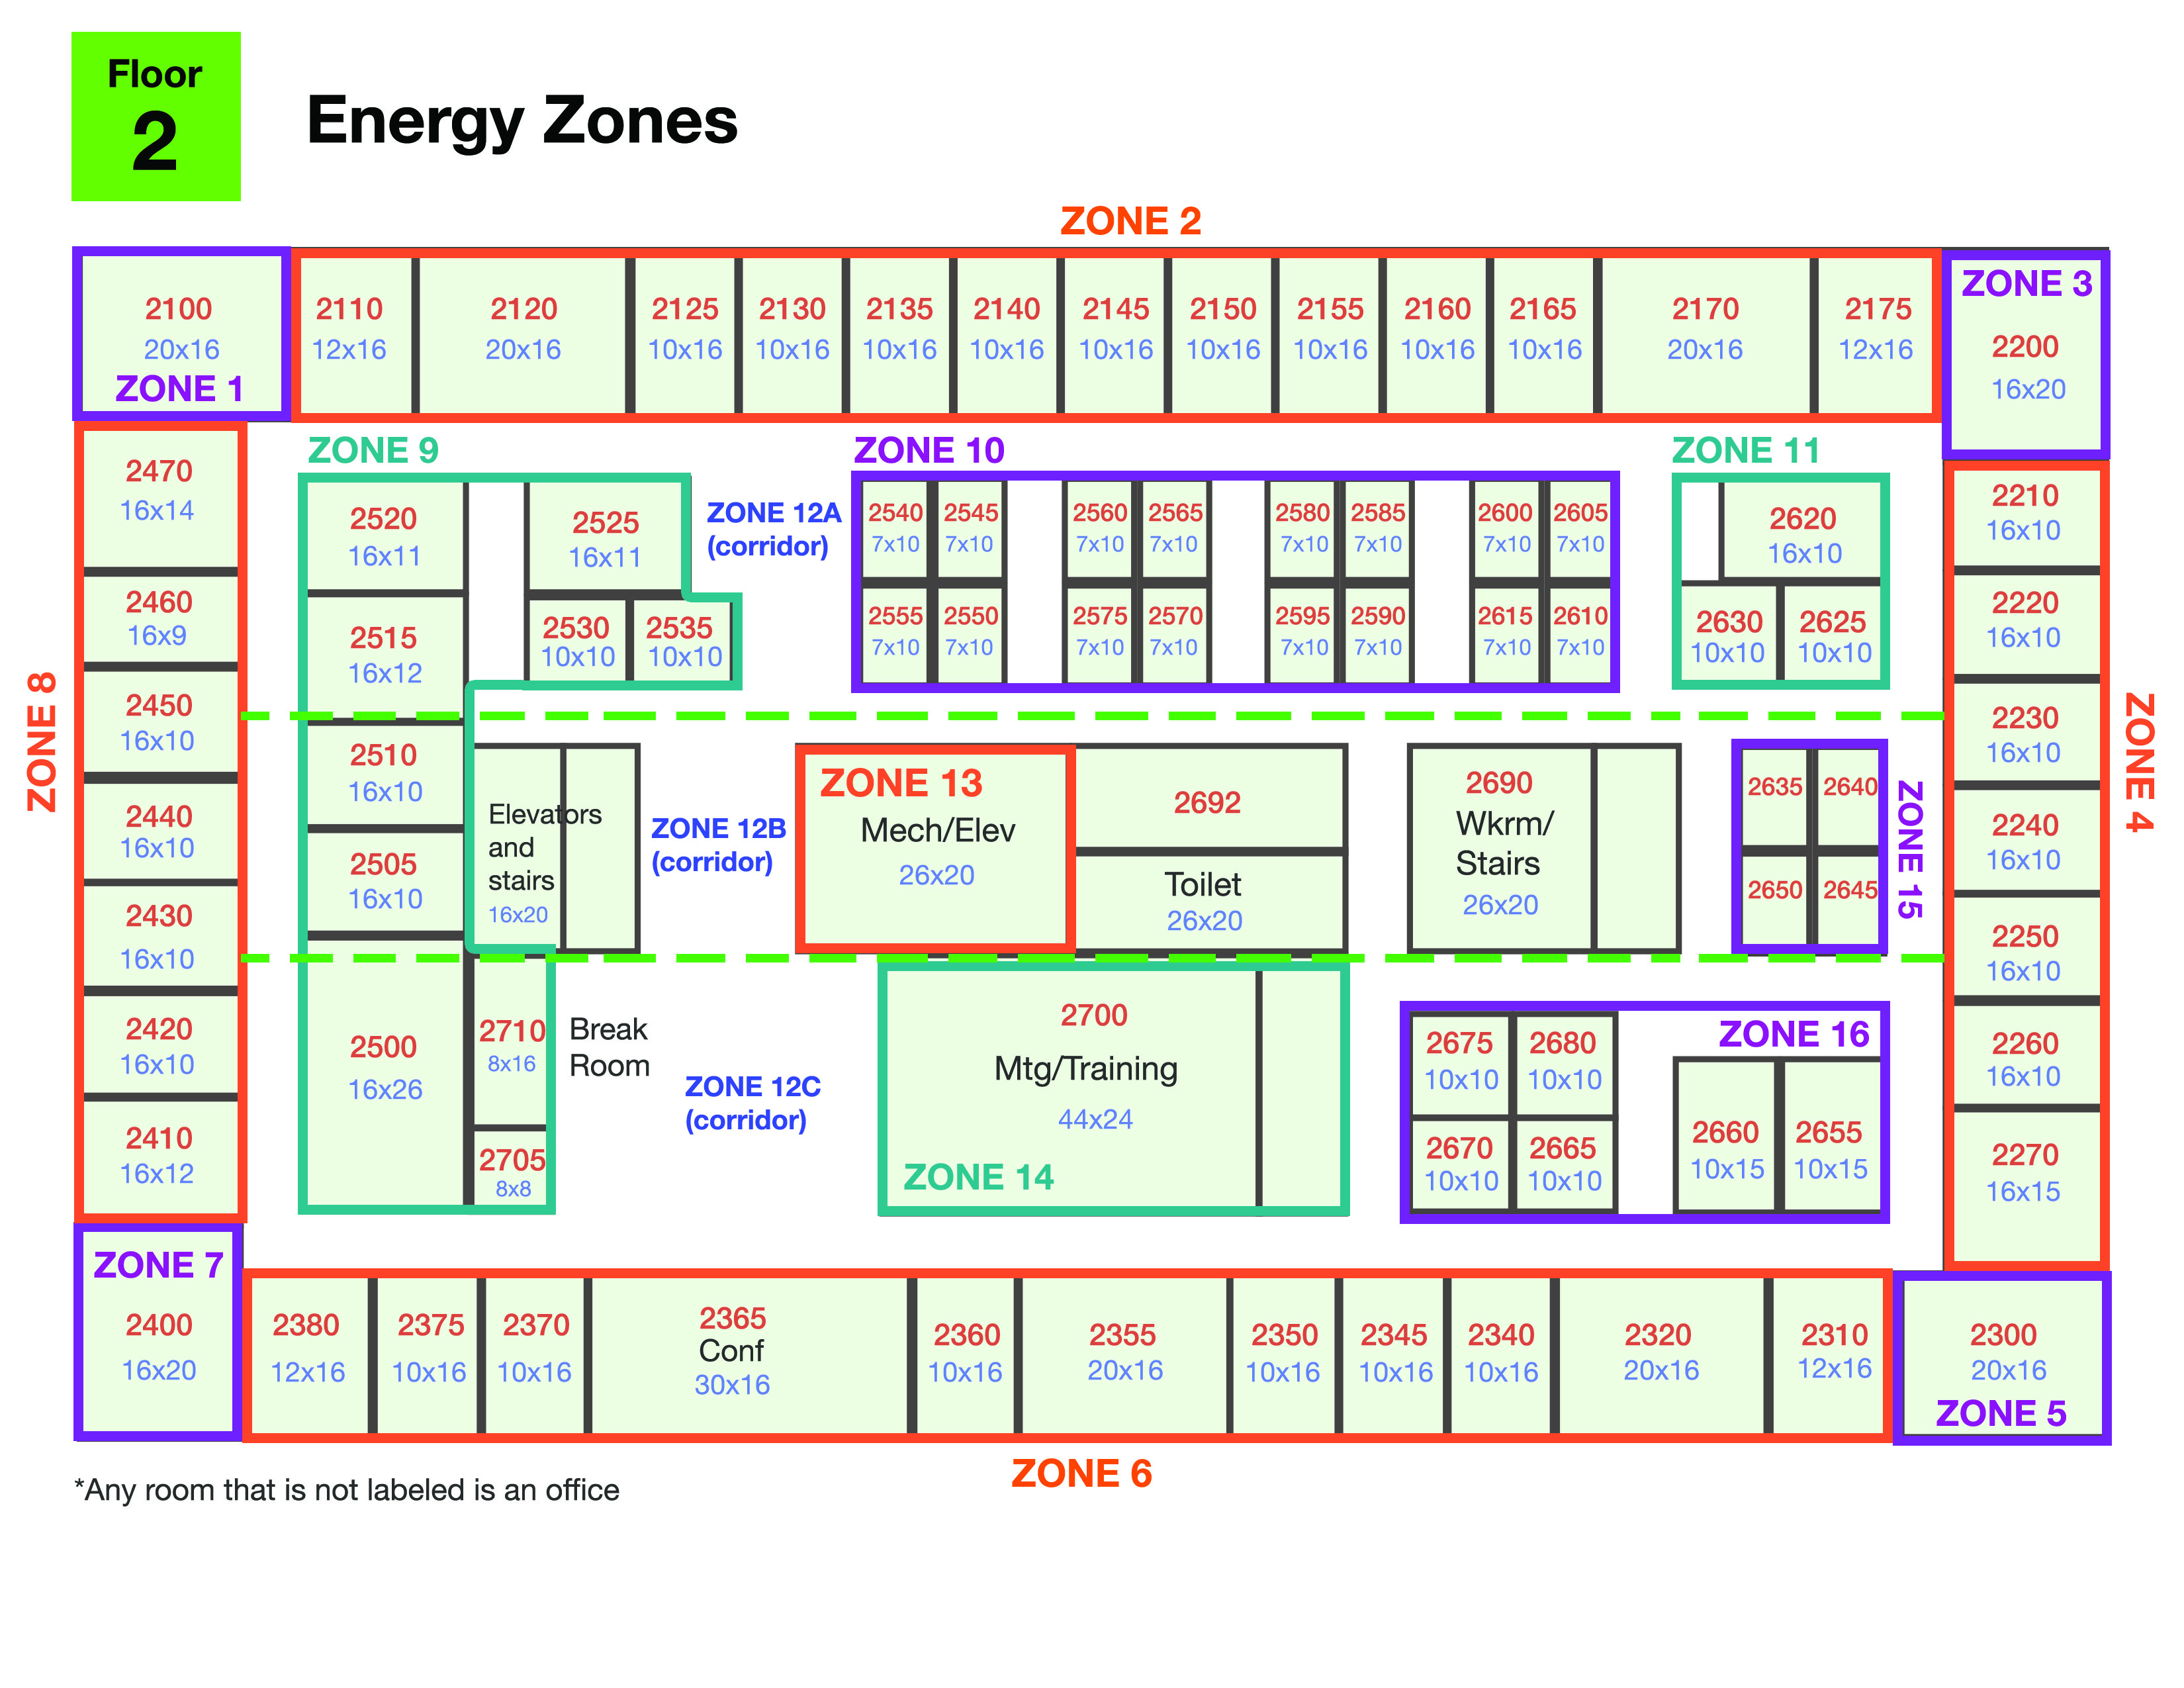
\includegraphics[width=0.3 \linewidth]{figures/energy2.jpg}
                        &
                        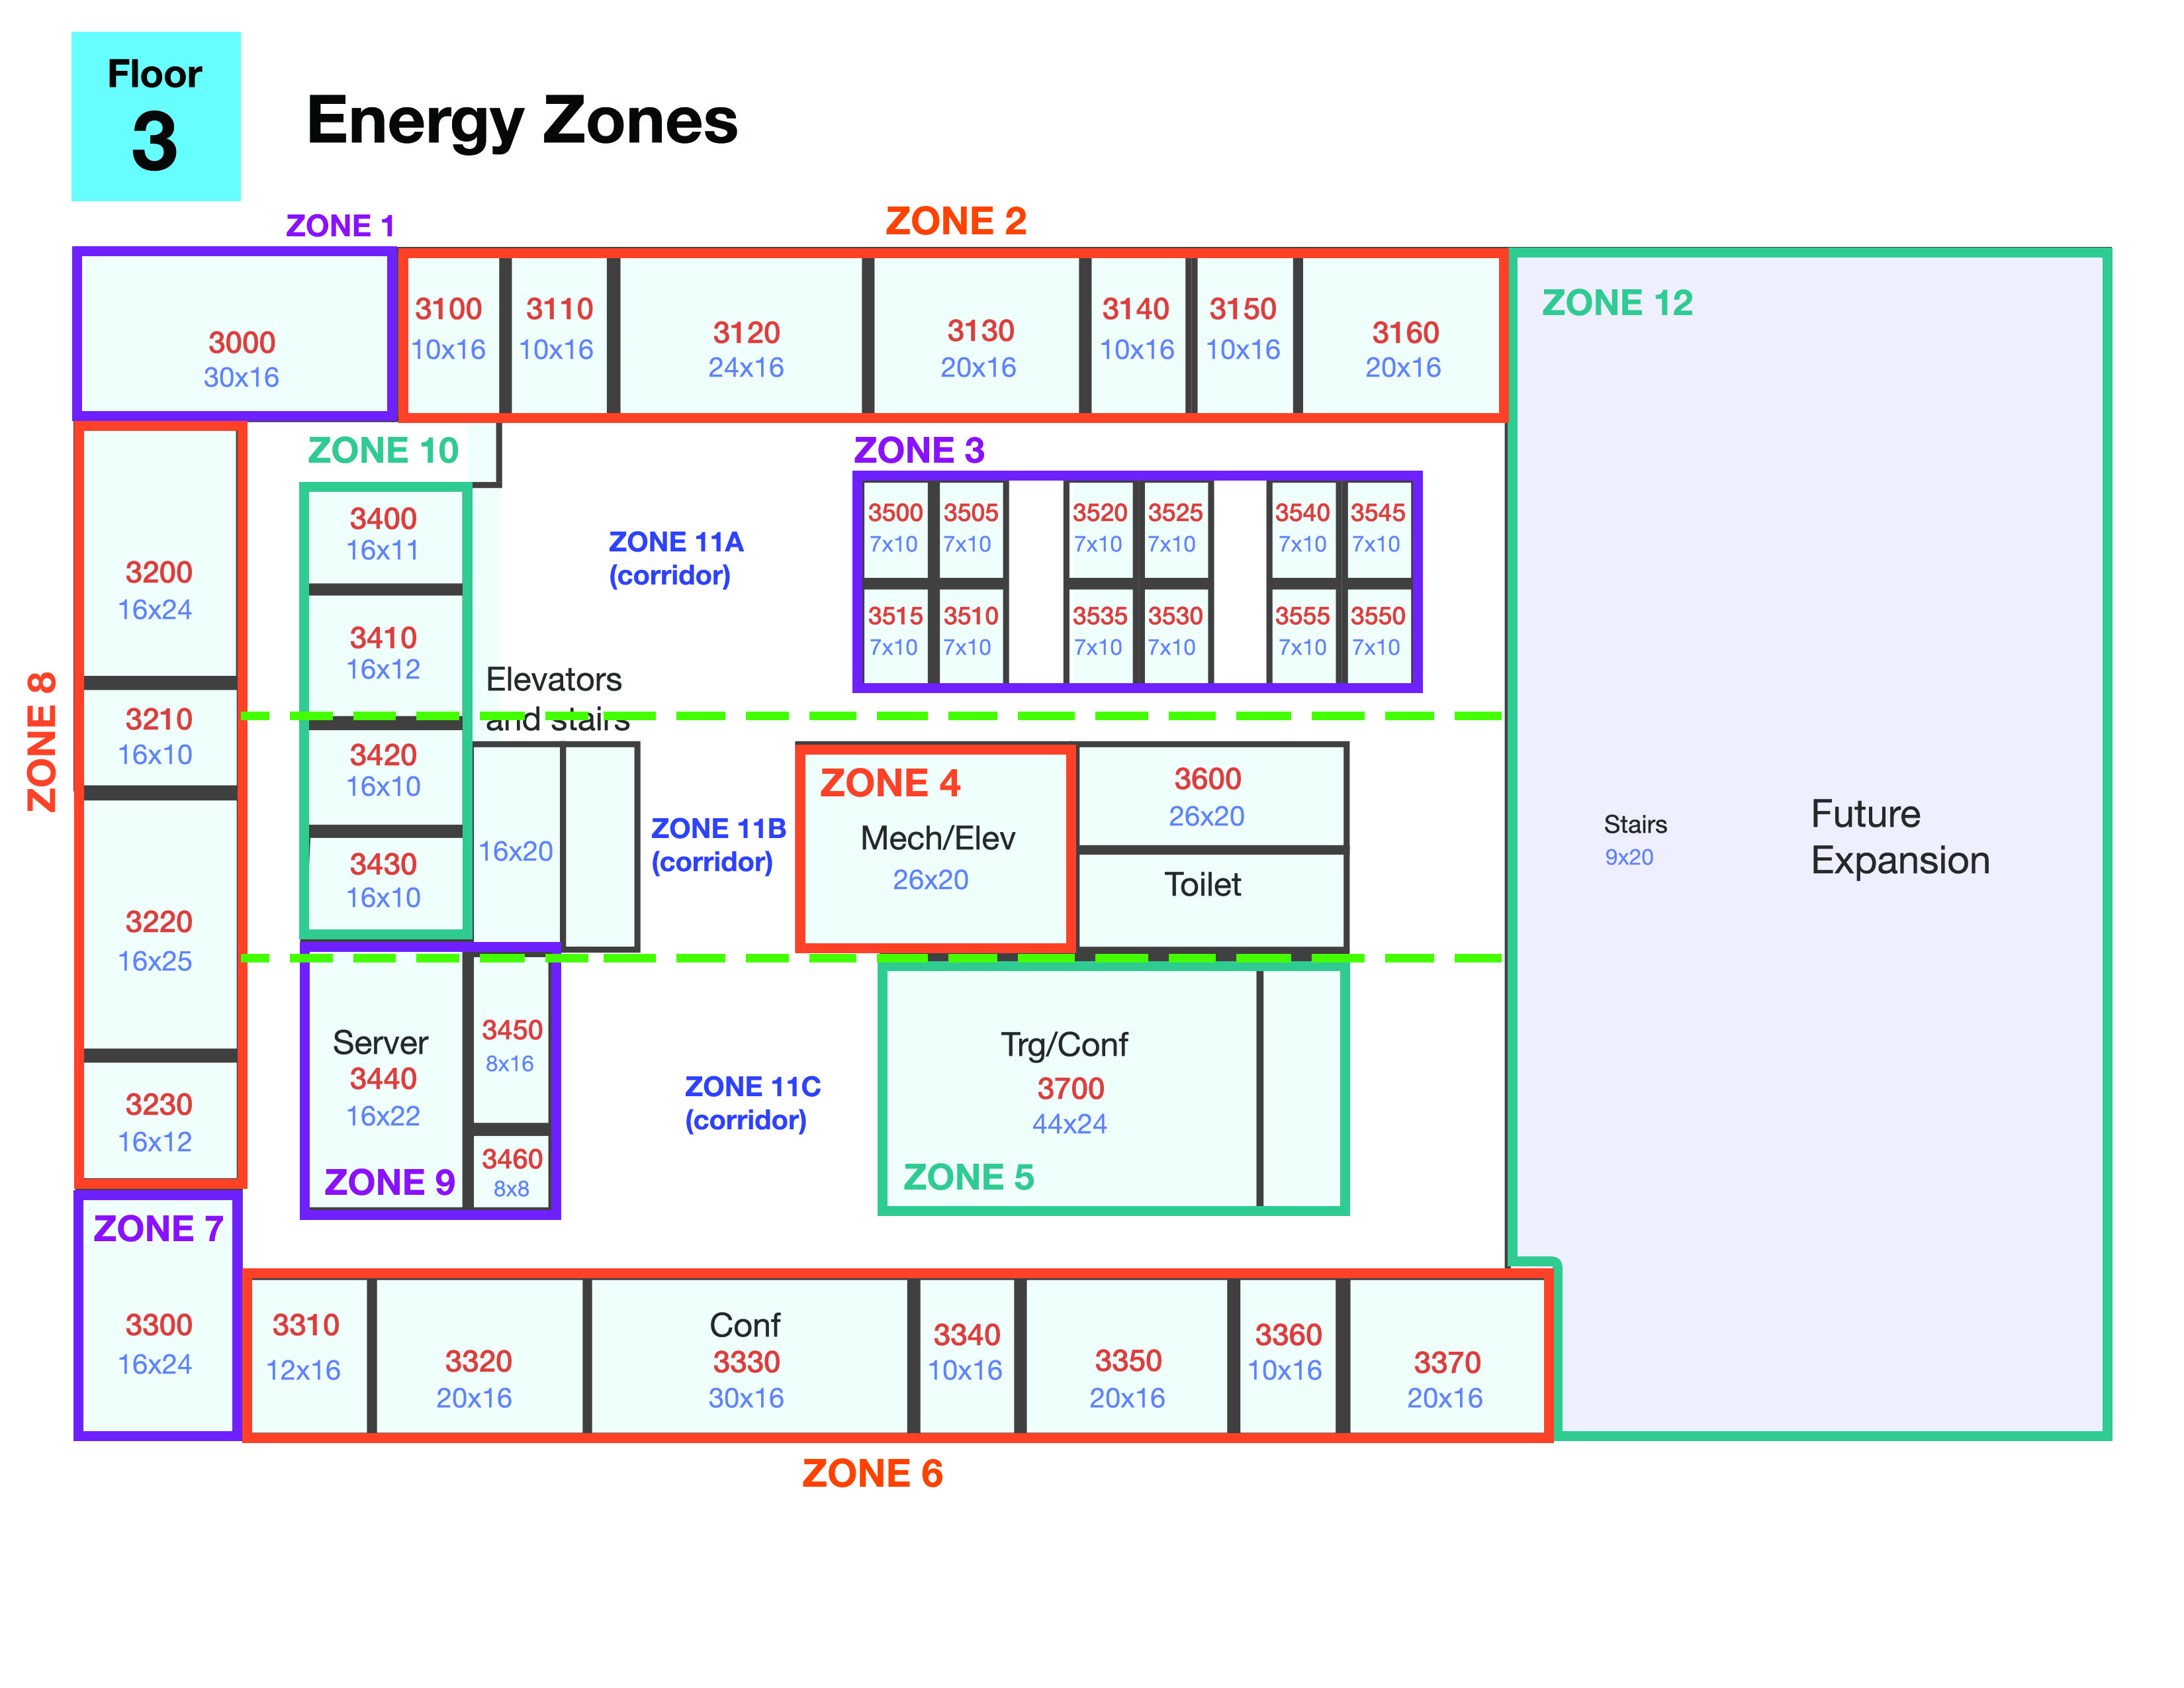
\includegraphics[width=0.3 \linewidth]{figures/energy3.jpg}
                        \\
                        
                        \mbox{(a) First Floor} & \mbox{(b) Second Floor} & \mbox{(c) Third Floor} \\
                    \end{array}$
                    \caption{Energy Zone of the Building}
                    \label{fig:energy}
                \end{figure}
            
                The energy zone of this building is as figure \ref{fig:energy}. 
                
            \subsubsection{Prox Zone Layout}
                \begin{figure}[htbp]
                    \centering
                    $\begin{array}{ccc}
                        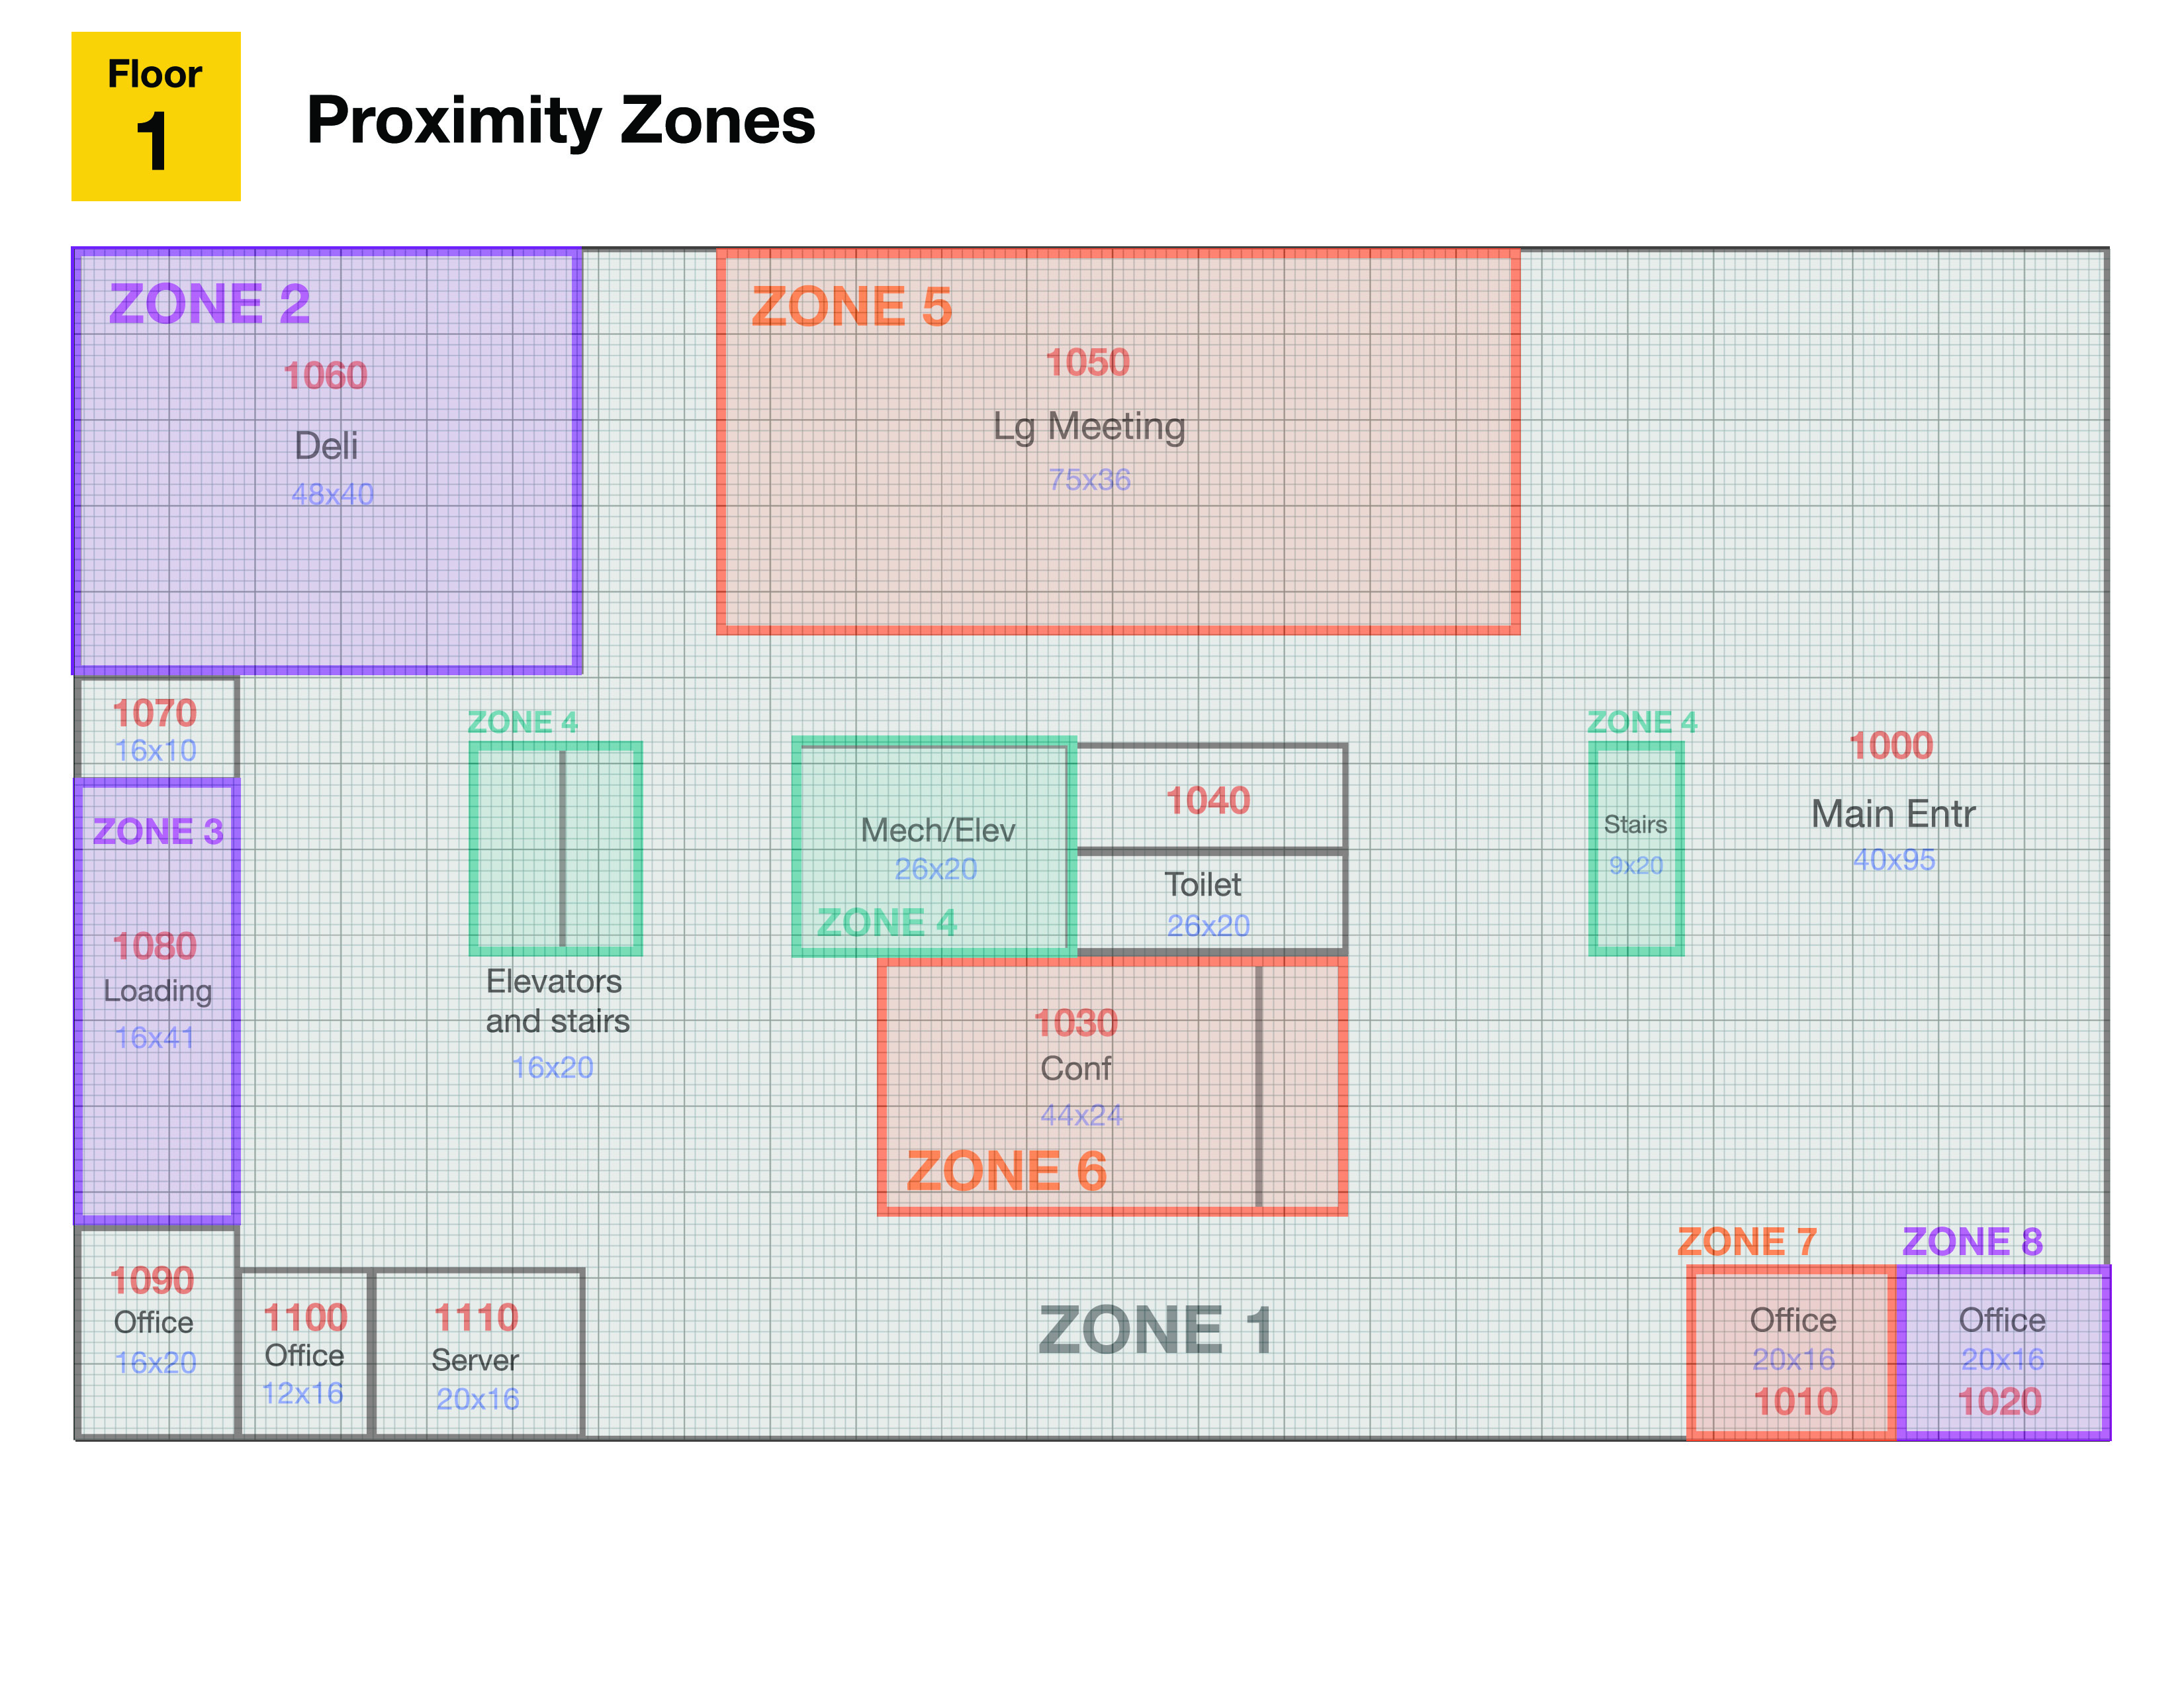
\includegraphics[width=0.3 \linewidth]{figures/prox1.jpg}
                        &
                        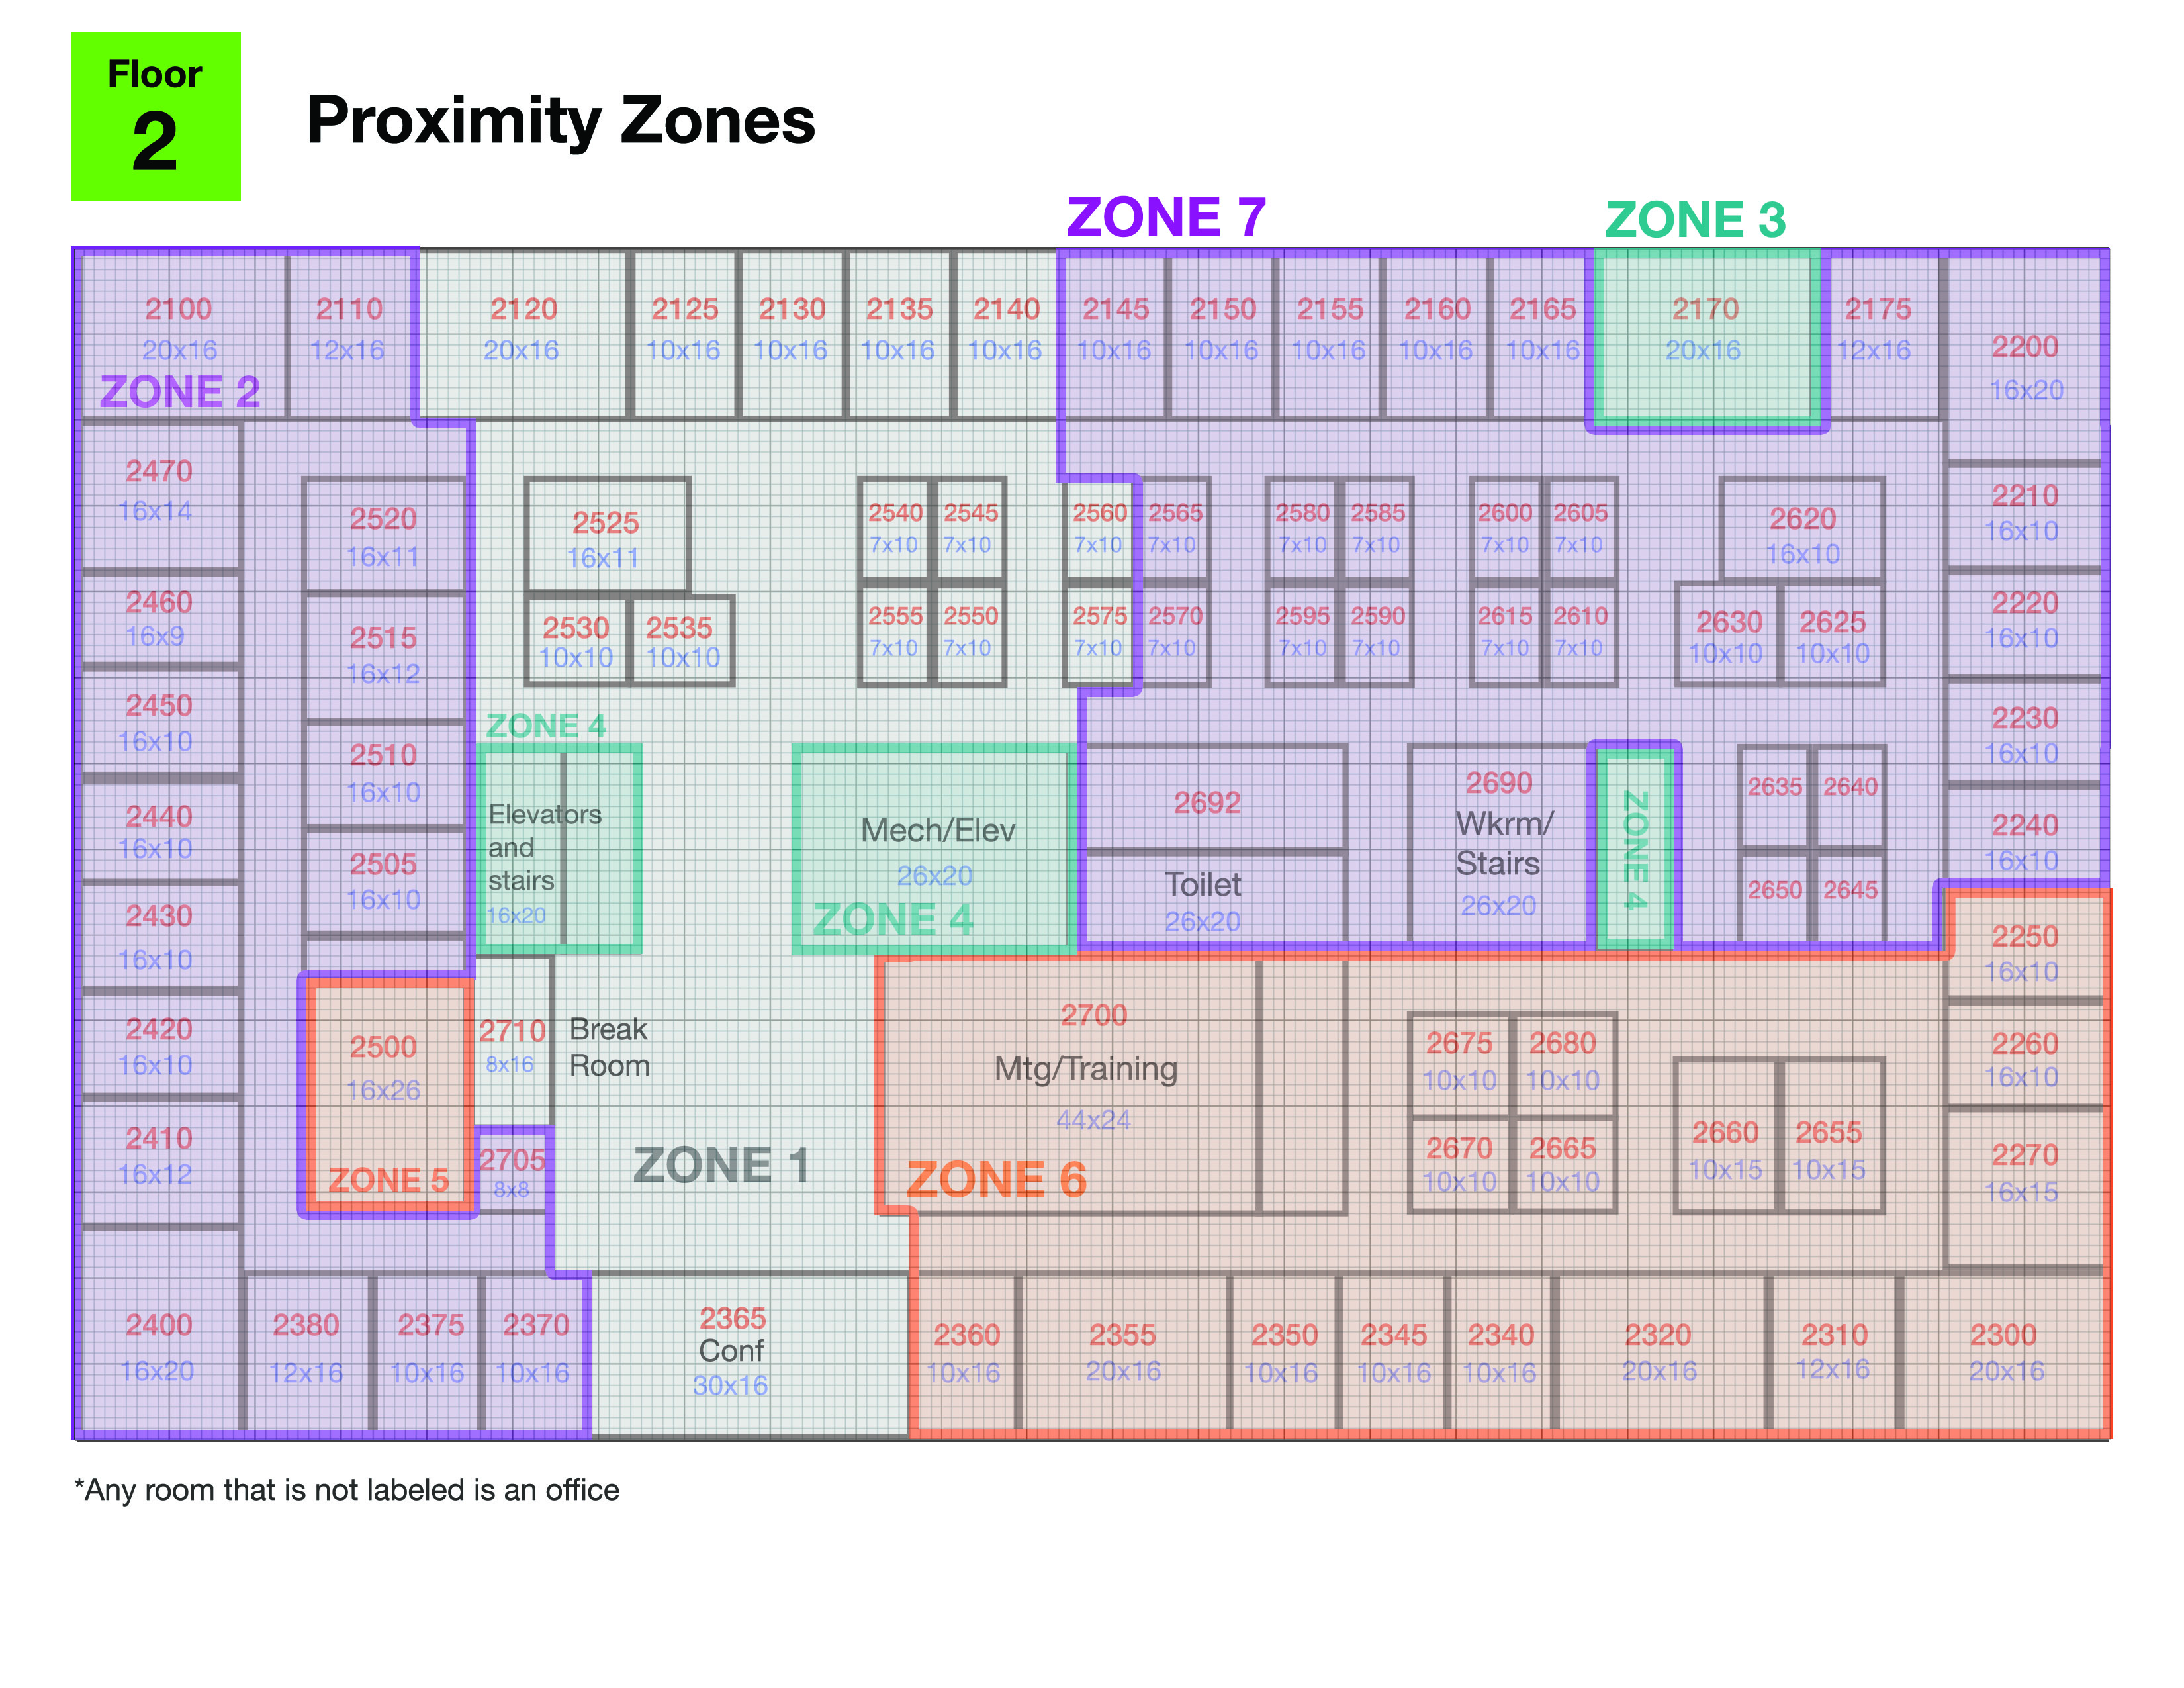
\includegraphics[width=0.3 \linewidth]{figures/prox2.jpg}
                        &
                        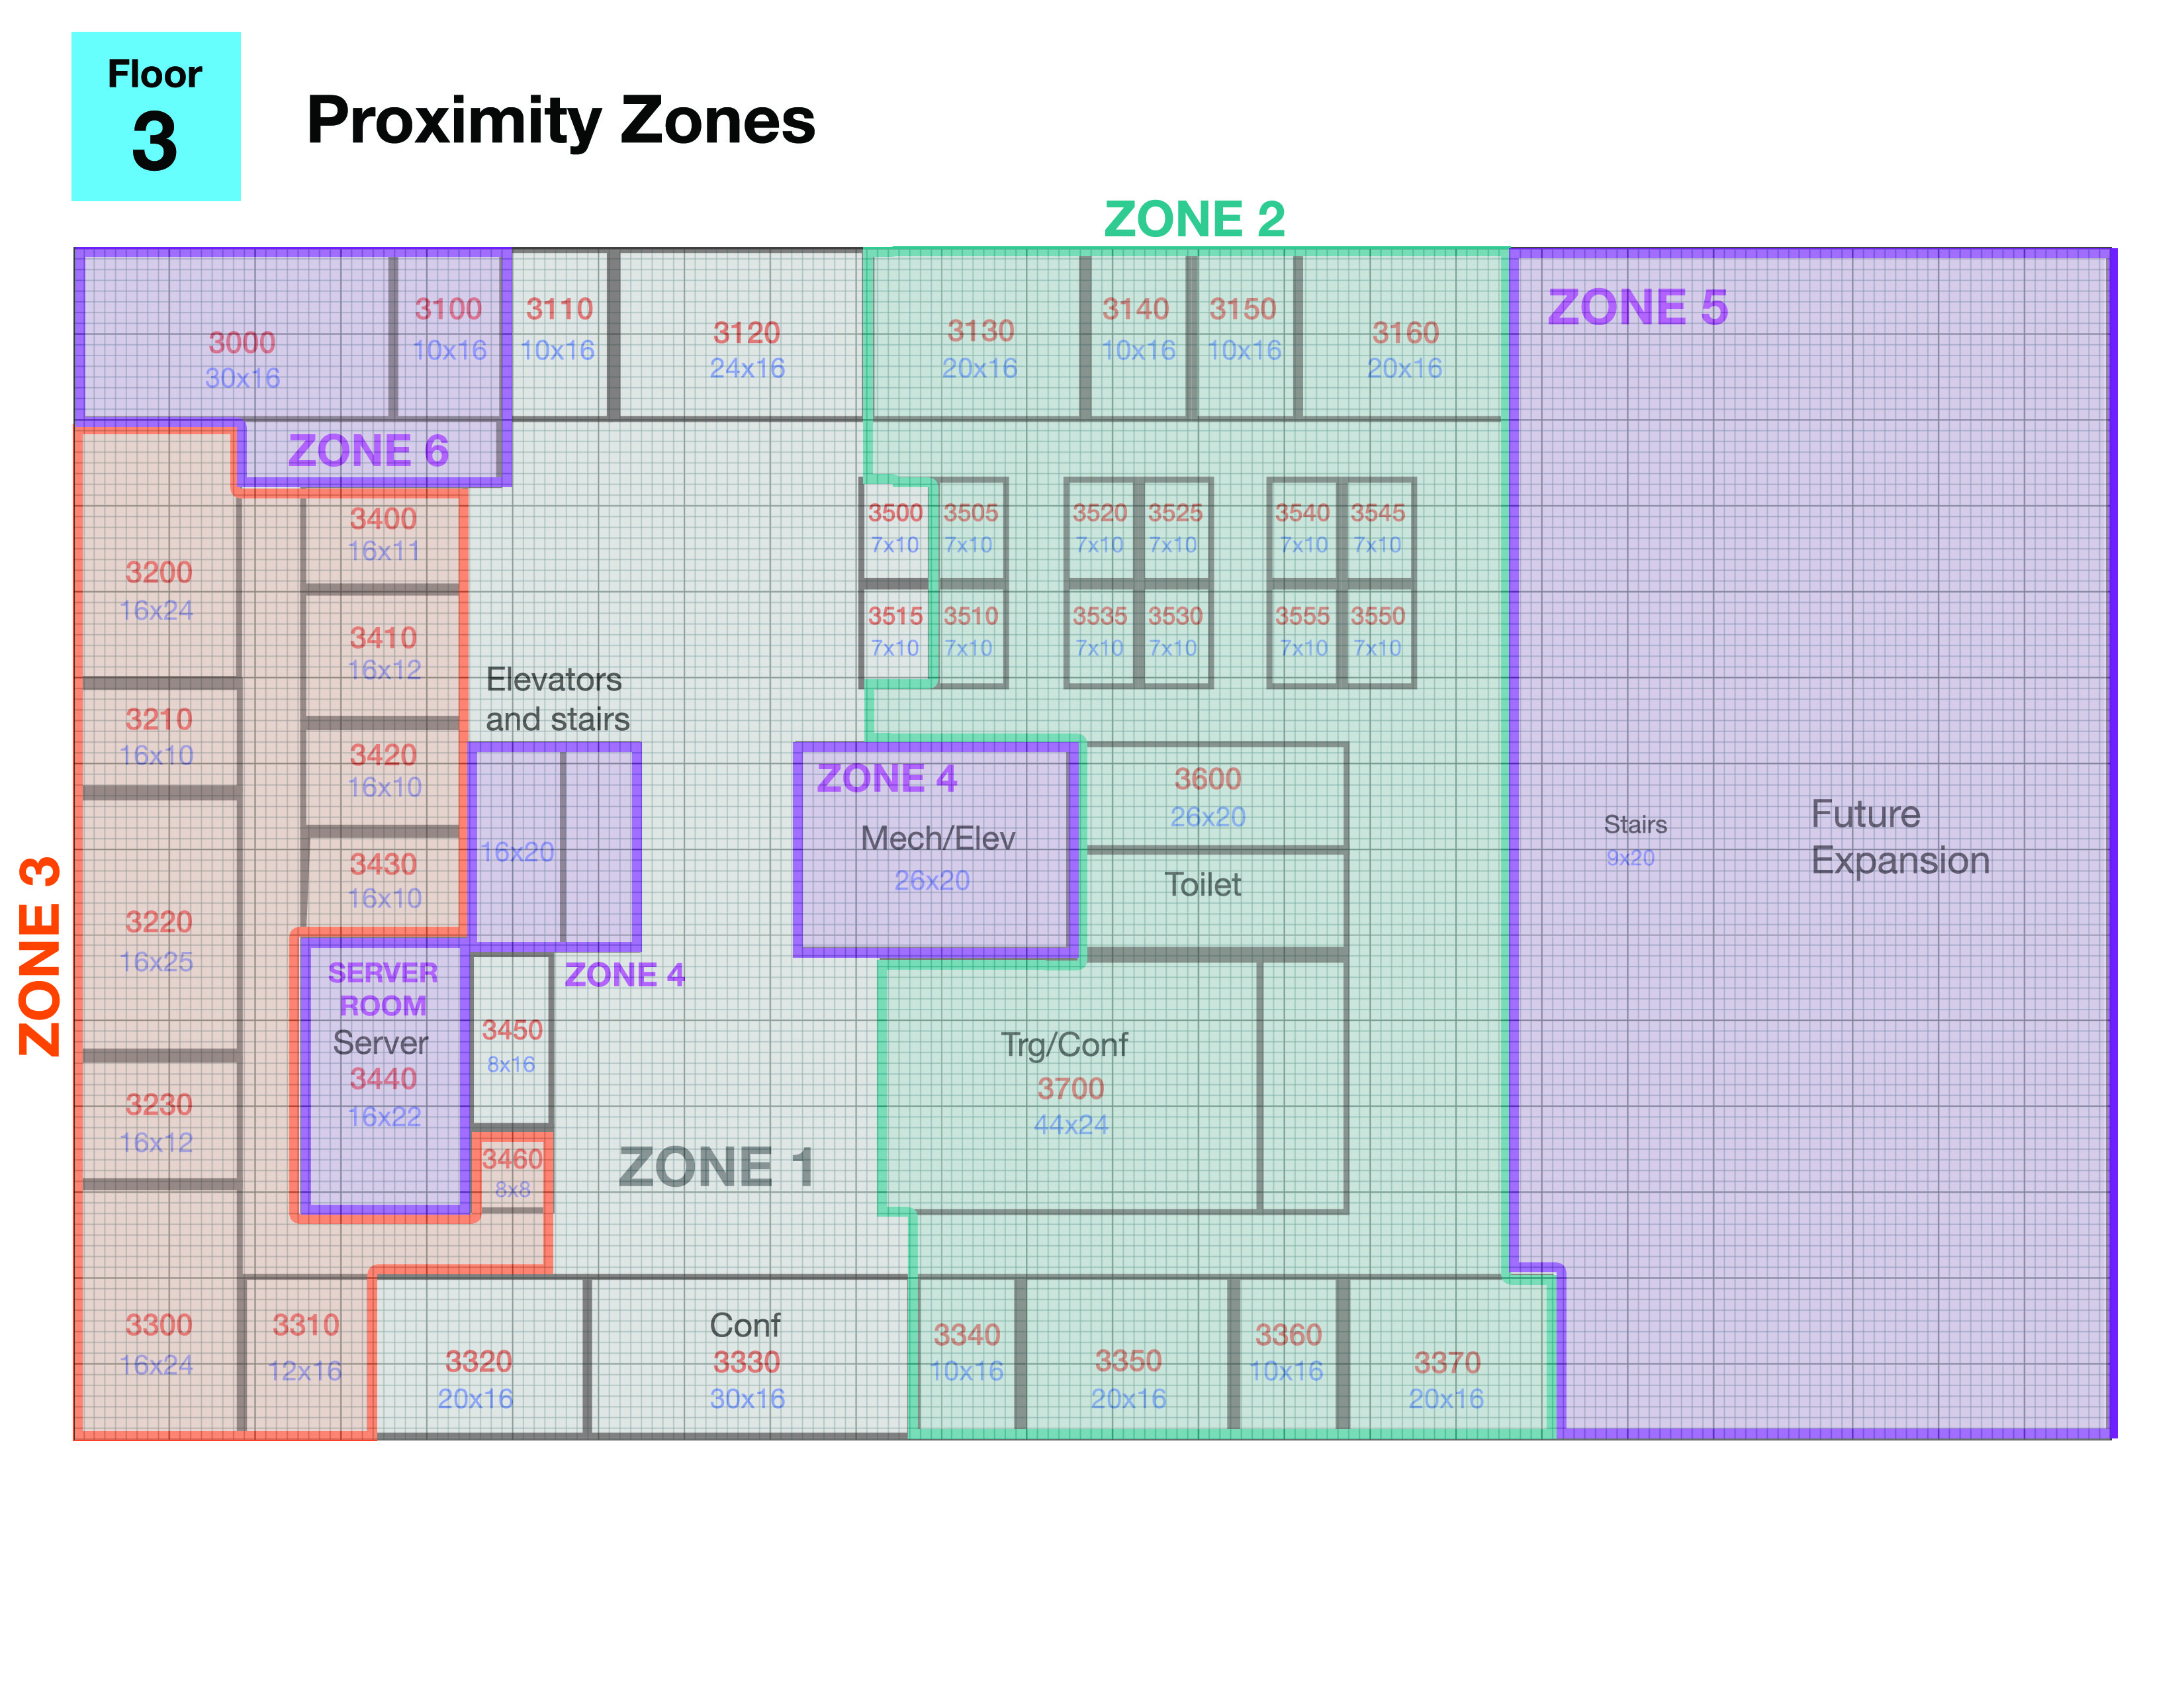
\includegraphics[width=0.3 \linewidth]{figures/prox3.jpg}
                        \\
                        
                        \mbox{(a) First Floor} & \mbox{(b) Second Floor} & \mbox{(c) Third Floor} \\
                    \end{array}$
                    \caption{Prox zone of the Building}
                    \label{fig:prox}
                \end{figure}
            
                The prox zone of this building is as figure \ref{fig:prox}.
    
    \section{Methods}
        \subsection{Python Packages}
            To analyze data, we used Python programming language. Also, we adopt many Python modules as hereinafter. 
        
            \subsubsection{Scikit-learn: Machine Learning in Python}
                \textit{Scikit-learn} is a Python module integrating a wide range of state-of-the-art machine learning algorithms for medium-scale supervised and unsupervised problems \cite{ref:sklearn1}.
                
            \subsubsection{Matplotlib}
                \textit{Matplotlib} is a Python 2D plotting library which produces publication quality figures in a variety of hardcopy formats and interactive environments across platforms \cite{ref:matplotlib1}.
                
            \subsubsection{Pandas}
                \textit{Pandas} is a Python library of rich data structures and tools for working with structured data sets common to statistic, finance, social sciences, and many other fields \cite{ref:pandas1}.
                
            \subsubsection{SciPy}
                \textit{SciPy} is a Python-based ecosystem of open-source software for mathematics, science, and engineering \cite{ref:scipy1}.
                
            \subsubsection{Pillow}
                \textit{Pillow} is the Python Imaging Library. \cite{ref:pil1}
                
         \subsection{JavaScript}
            For implementing interactive plots in web, we used JavaScript for showing plots. 
            
            \subsubsection{Plotly}
                \textit{Plotly} is a high-level, declarative charting library. plotly.js ships with over 40 chart types, including 3D charts, statistical graphs, and SVG maps. \cite{ref:plotly1}
                
        \subsection{TSNE}
            T-distributed Stochastic Neighbor Embedding (TSNE) is a machine learning algorithm for visualization high-dimensional data in a low-dimensional space \cite{ref:tsne1}.
         
        \subsection{Standardization}
            Note that, in this analysis, all values are standardized. In other words, all values are adjusted for the mean value is zero, and standard deviation is 1. If all values in one columns are same, then the column will be discarded. 
    
    \section{Results}
        \subsection[Question 1]{What are the typical patterns in the prox card data? What does a typical day look like for GAStech employees?}
            \label{sec:question1}
            \subsubsection{General Information of prox Data}
                First of all, we drew the distribution of movement distance as figure \ref{fig:movementdist}. Also, the basic statistics values, such as minimum, maximum, and average, of movement distance is in table \ref{tb:movementdist}.
            
                \begin{figure}[htbp]
                    \centering
                    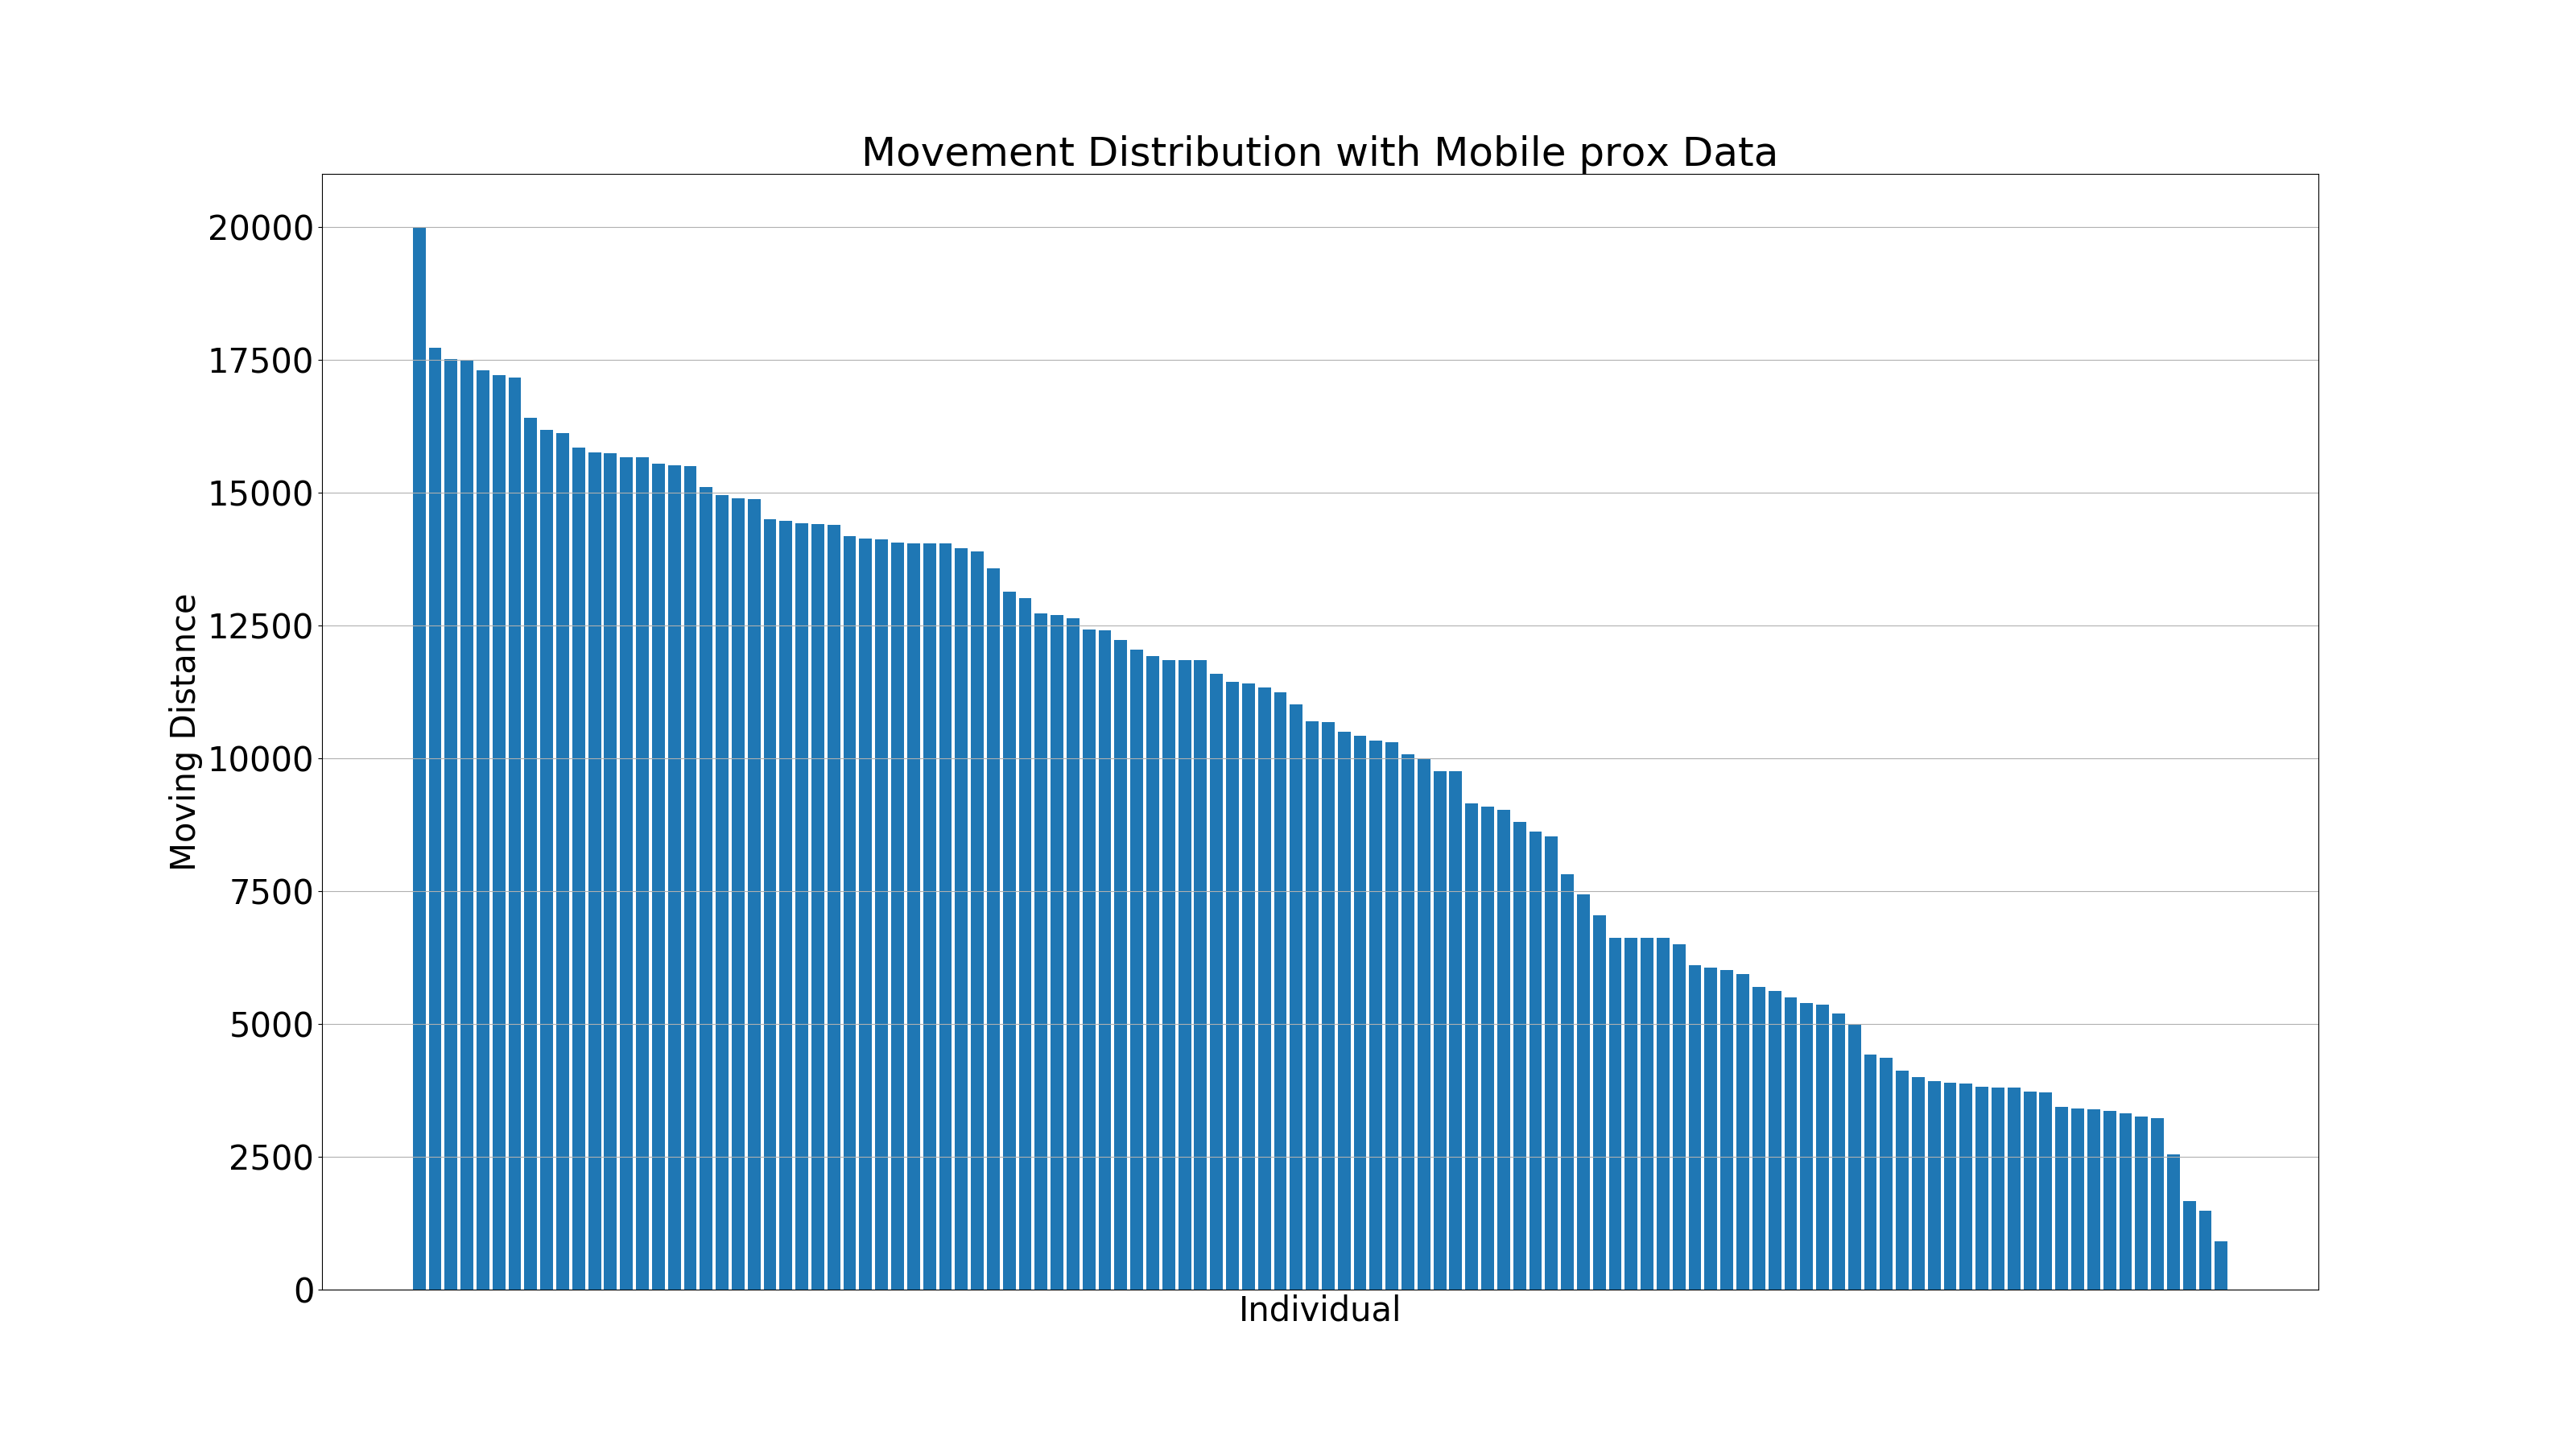
\includegraphics[width=0.6 \linewidth]{figures/movementdistribution.png}
                    \caption{Distribution of Movement Distance}
                    \label{fig:movementdist}
                \end{figure}
        
                \begin{table}[htbp]
                    \centering
                    \caption{Basic Statistics Data within Movement Distance}
                    \label{tb:movementdist}
                    \begin{tabular}{c||c|c|c|c|c|c|c}
                        Item & Minimum & Maximum & Mean & q1 & Median & q3 & Standard Deviation \\ \hline
                        Value & 902.44 & 19999.38 & 10083.95 & 5642.54 & 10688.57 & 14134.16 & 4750.46 \\
                    \end{tabular}
                \end{table}
            
                Furthermore, the extreme value of moving information is in tables \ref{tb:movemin} and \ref{tb:movemax}.
                
                \begin{table}[htbp]
                    \centering
                    \caption{Minimum Moving Employees}
                    \label{tb:movemin}
                    \begin{tabular}{c|c}
                        Moving Distance & ID \\ \hline
                        902.4411338142776 & earpa \\
                        1482.4411338142788 & vawelon \\
                        1667.820095117141 & jfrost \\
                        2550.198060545332 & ibarranco \\
                        3233.4833039729083 & cstaley \\
                    \end{tabular}
                \end{table}
            
                \begin{table}[htbp]
                    \centering
                    \caption{Maximum Moving Employees}
                    \label{tb:movemax}
                    \begin{tabular}{c|c}
                        Moving Distance & ID \\ \hline
                        19999.386059326014 & chawelon \\
                        17719.3756100877 & hmies \\
                        17507.957735800737 & eminto \\
                        17478.788651971503 & monda \\
                        17302.863257165674 & ldedos \\
                    \end{tabular}
                \end{table}
            
            \subsubsection{Workflow}
                With the general information of prox data, we have decided our workflow for question 1 as figure \ref{fig:workflow1}.
                
                \begin{figure}[htbp]
                    \centering
                    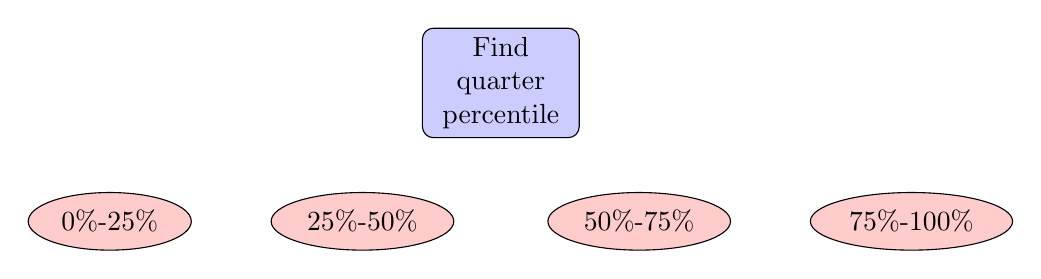
\begin{tikzpicture}[node distance = 2cm, auto]
                        \node[block](root1){Find quarter percentile};
                        \node[cloud, below of=root1, left of=root1](q2){25\%-50\%};
                        \node[cloud, below of=root1, right of=root1](q3){50\%-75\%};
                        \node[cloud, left=1cm of q2](q1){0\%-25\%};
                        \node[cloud, right=1cm of q3](q4){75\%-100\%};
                    \end{tikzpicture}
                    \caption{Workflow for Question 1}
                    \label{fig:workflow1}
                \end{figure}
        
            \subsubsection{Movement Direction and Distance}
                We drew the plot about movement direction and distance with each sub-group as figures \ref{fig:movedd1}, \ref{fig:movedd2}, and \ref{fig:movedd3}. Note that the darkness of arrow is proportioned with number of duplicates. 
            
                \begin{figure}[htbp]
                    \centering
                    $\begin{array}{cc}
                        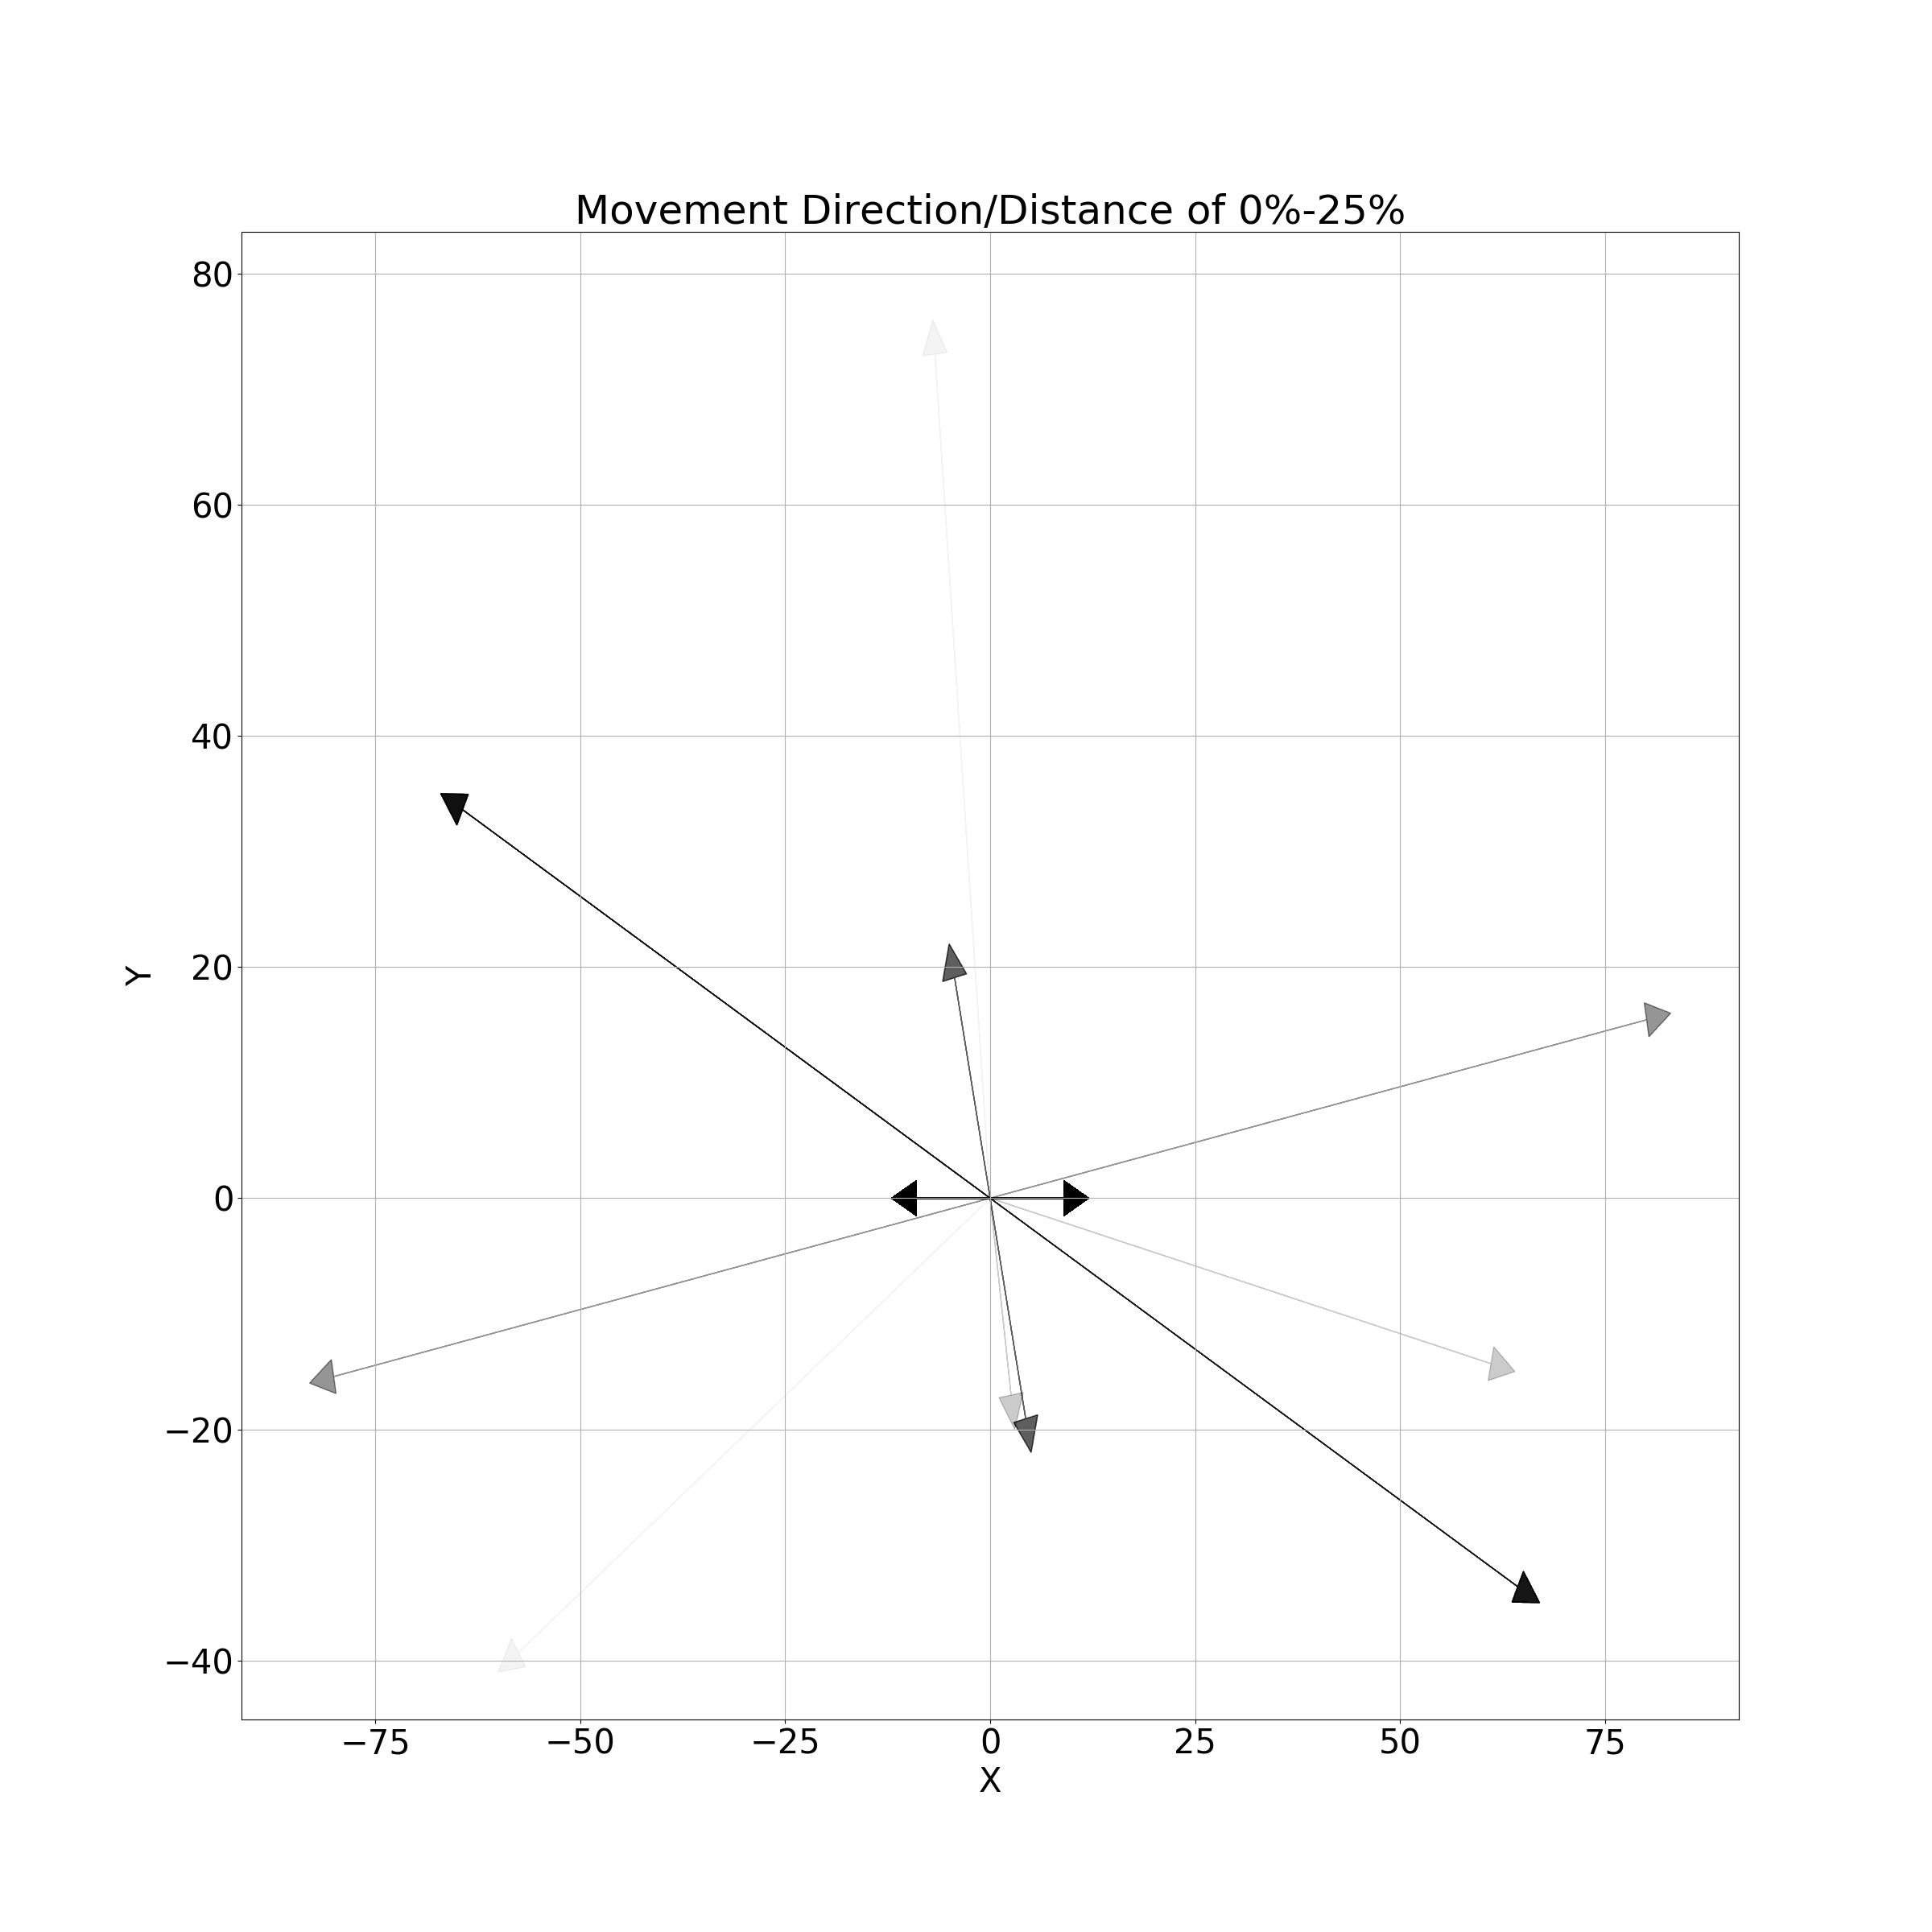
\includegraphics[width=0.3 \linewidth]{figures/movement1-1.png}
                        &
                        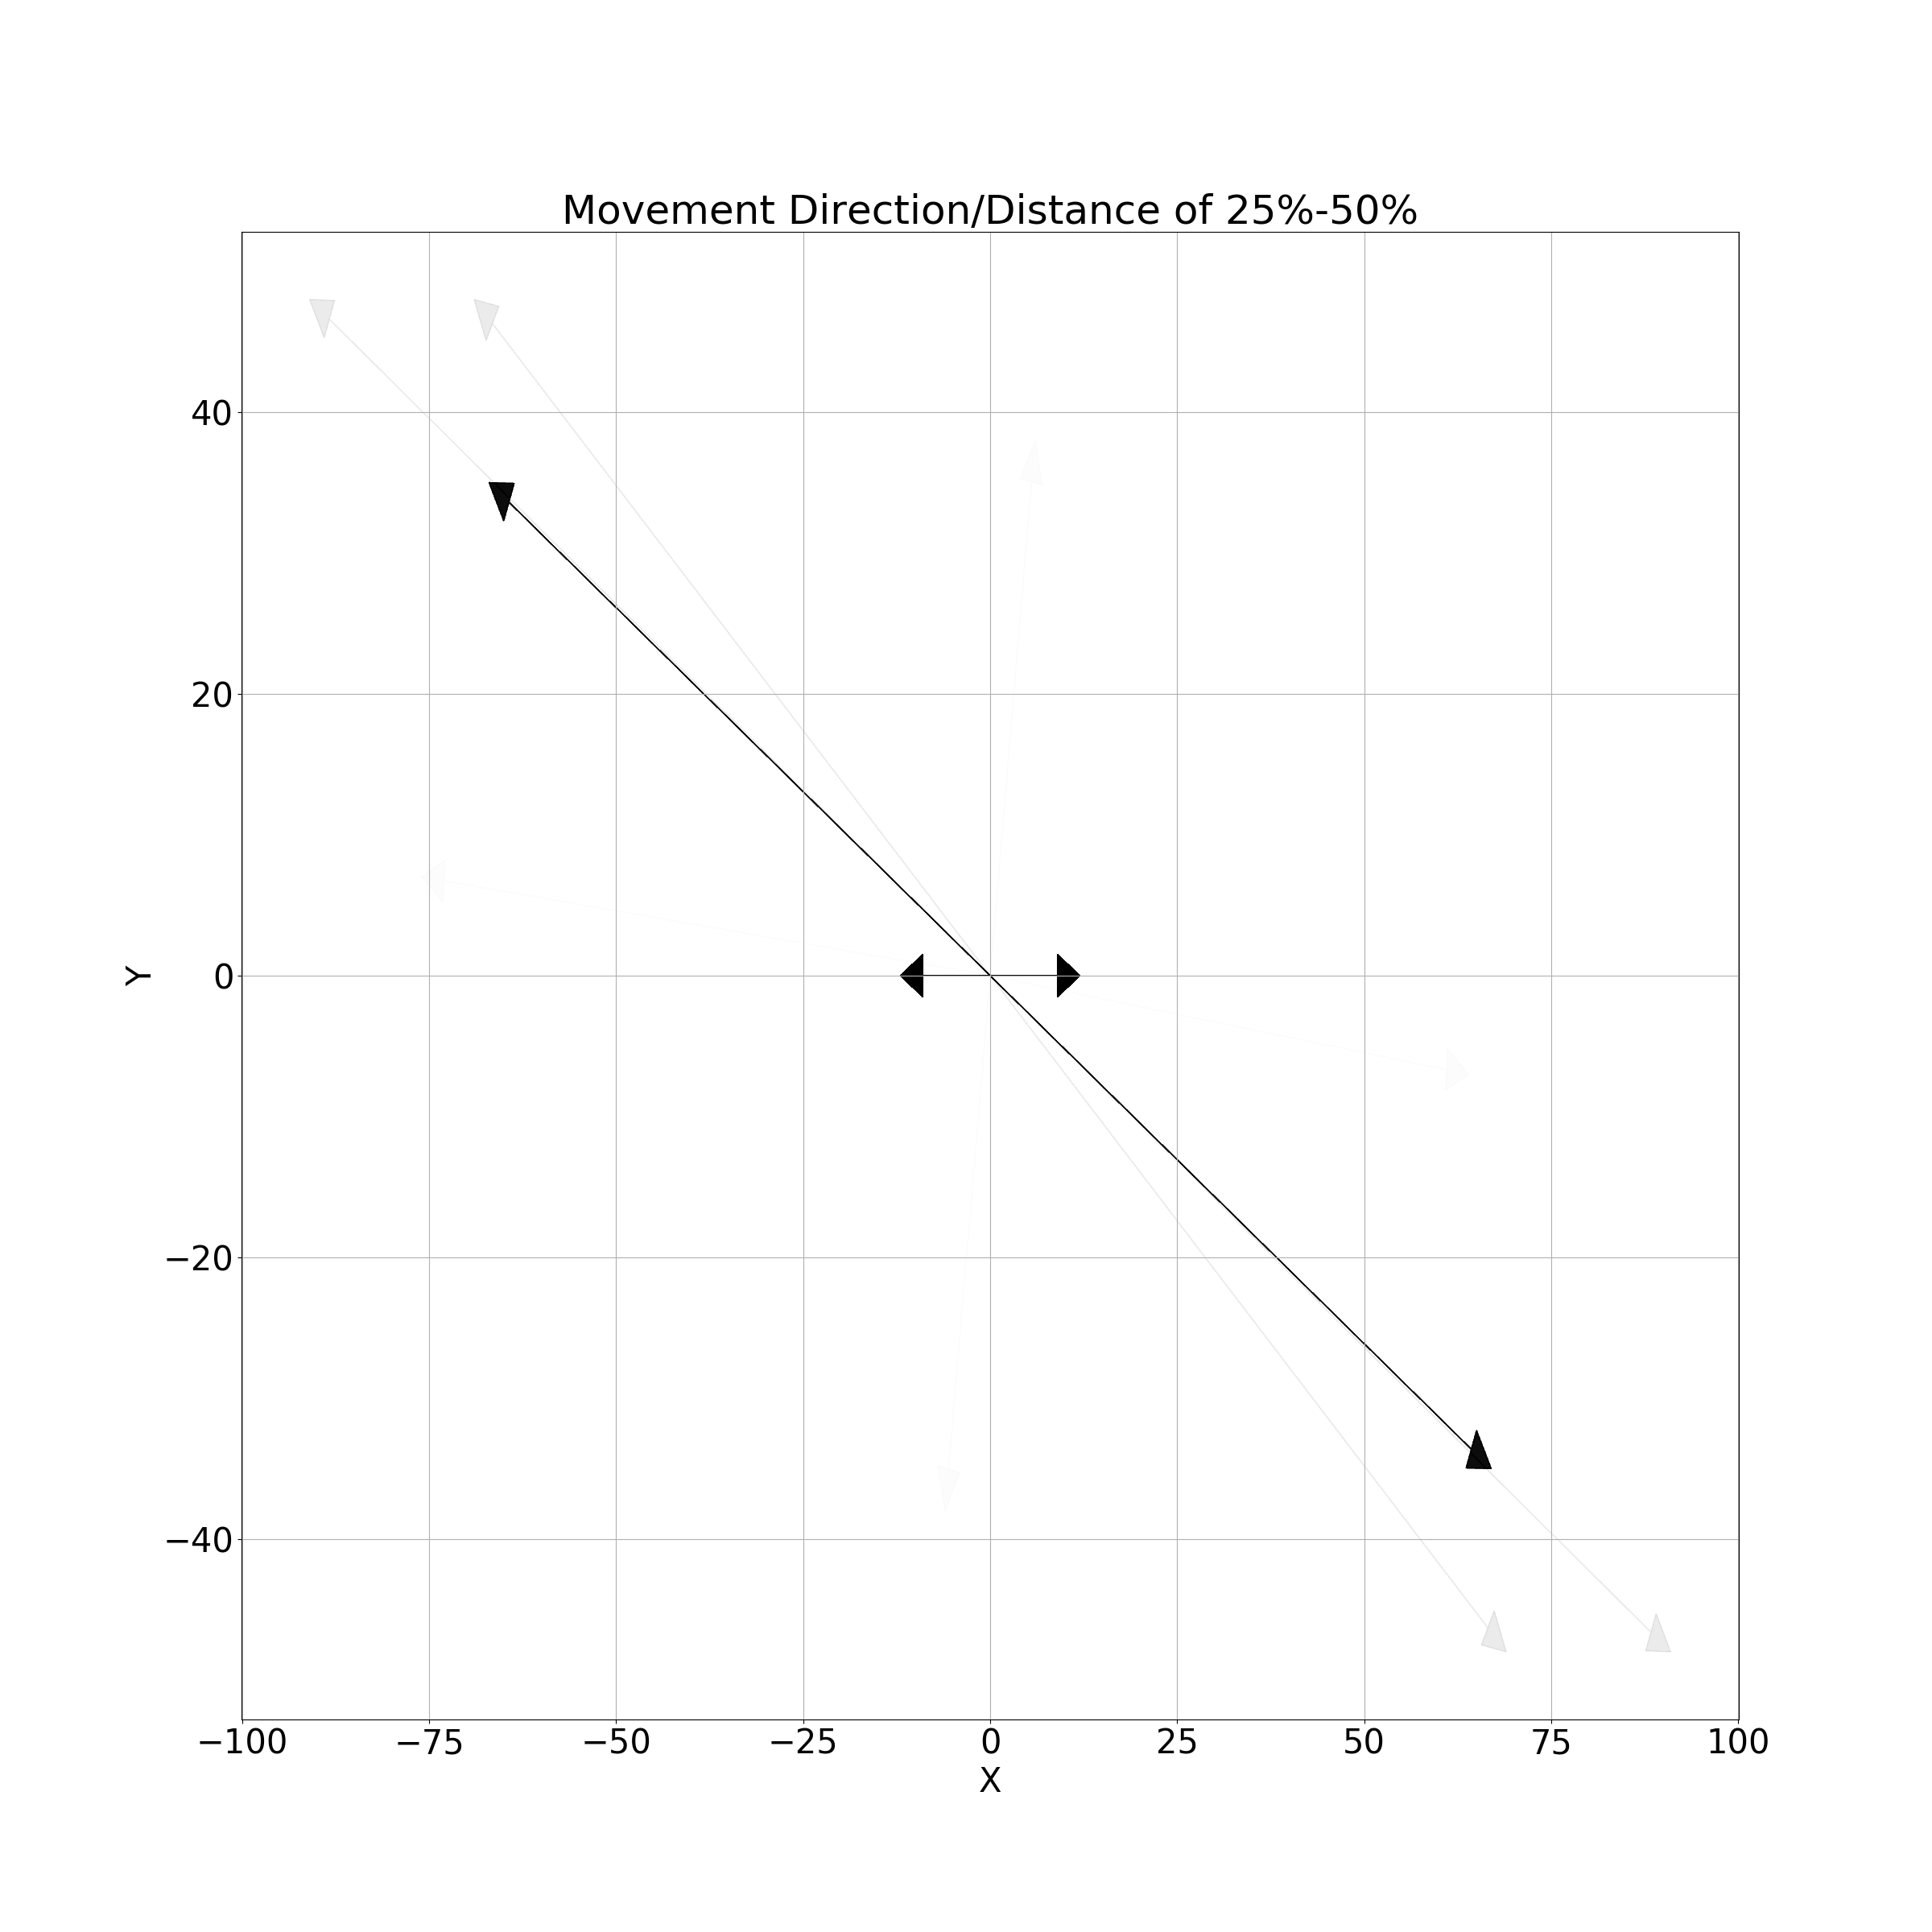
\includegraphics[width=0.3 \linewidth]{figures/movement1-2.png}
                        \\
                        
                        \mbox{(a) 0\%-25\%} & \mbox{(b) 25\%-50\%} \\
                        
                        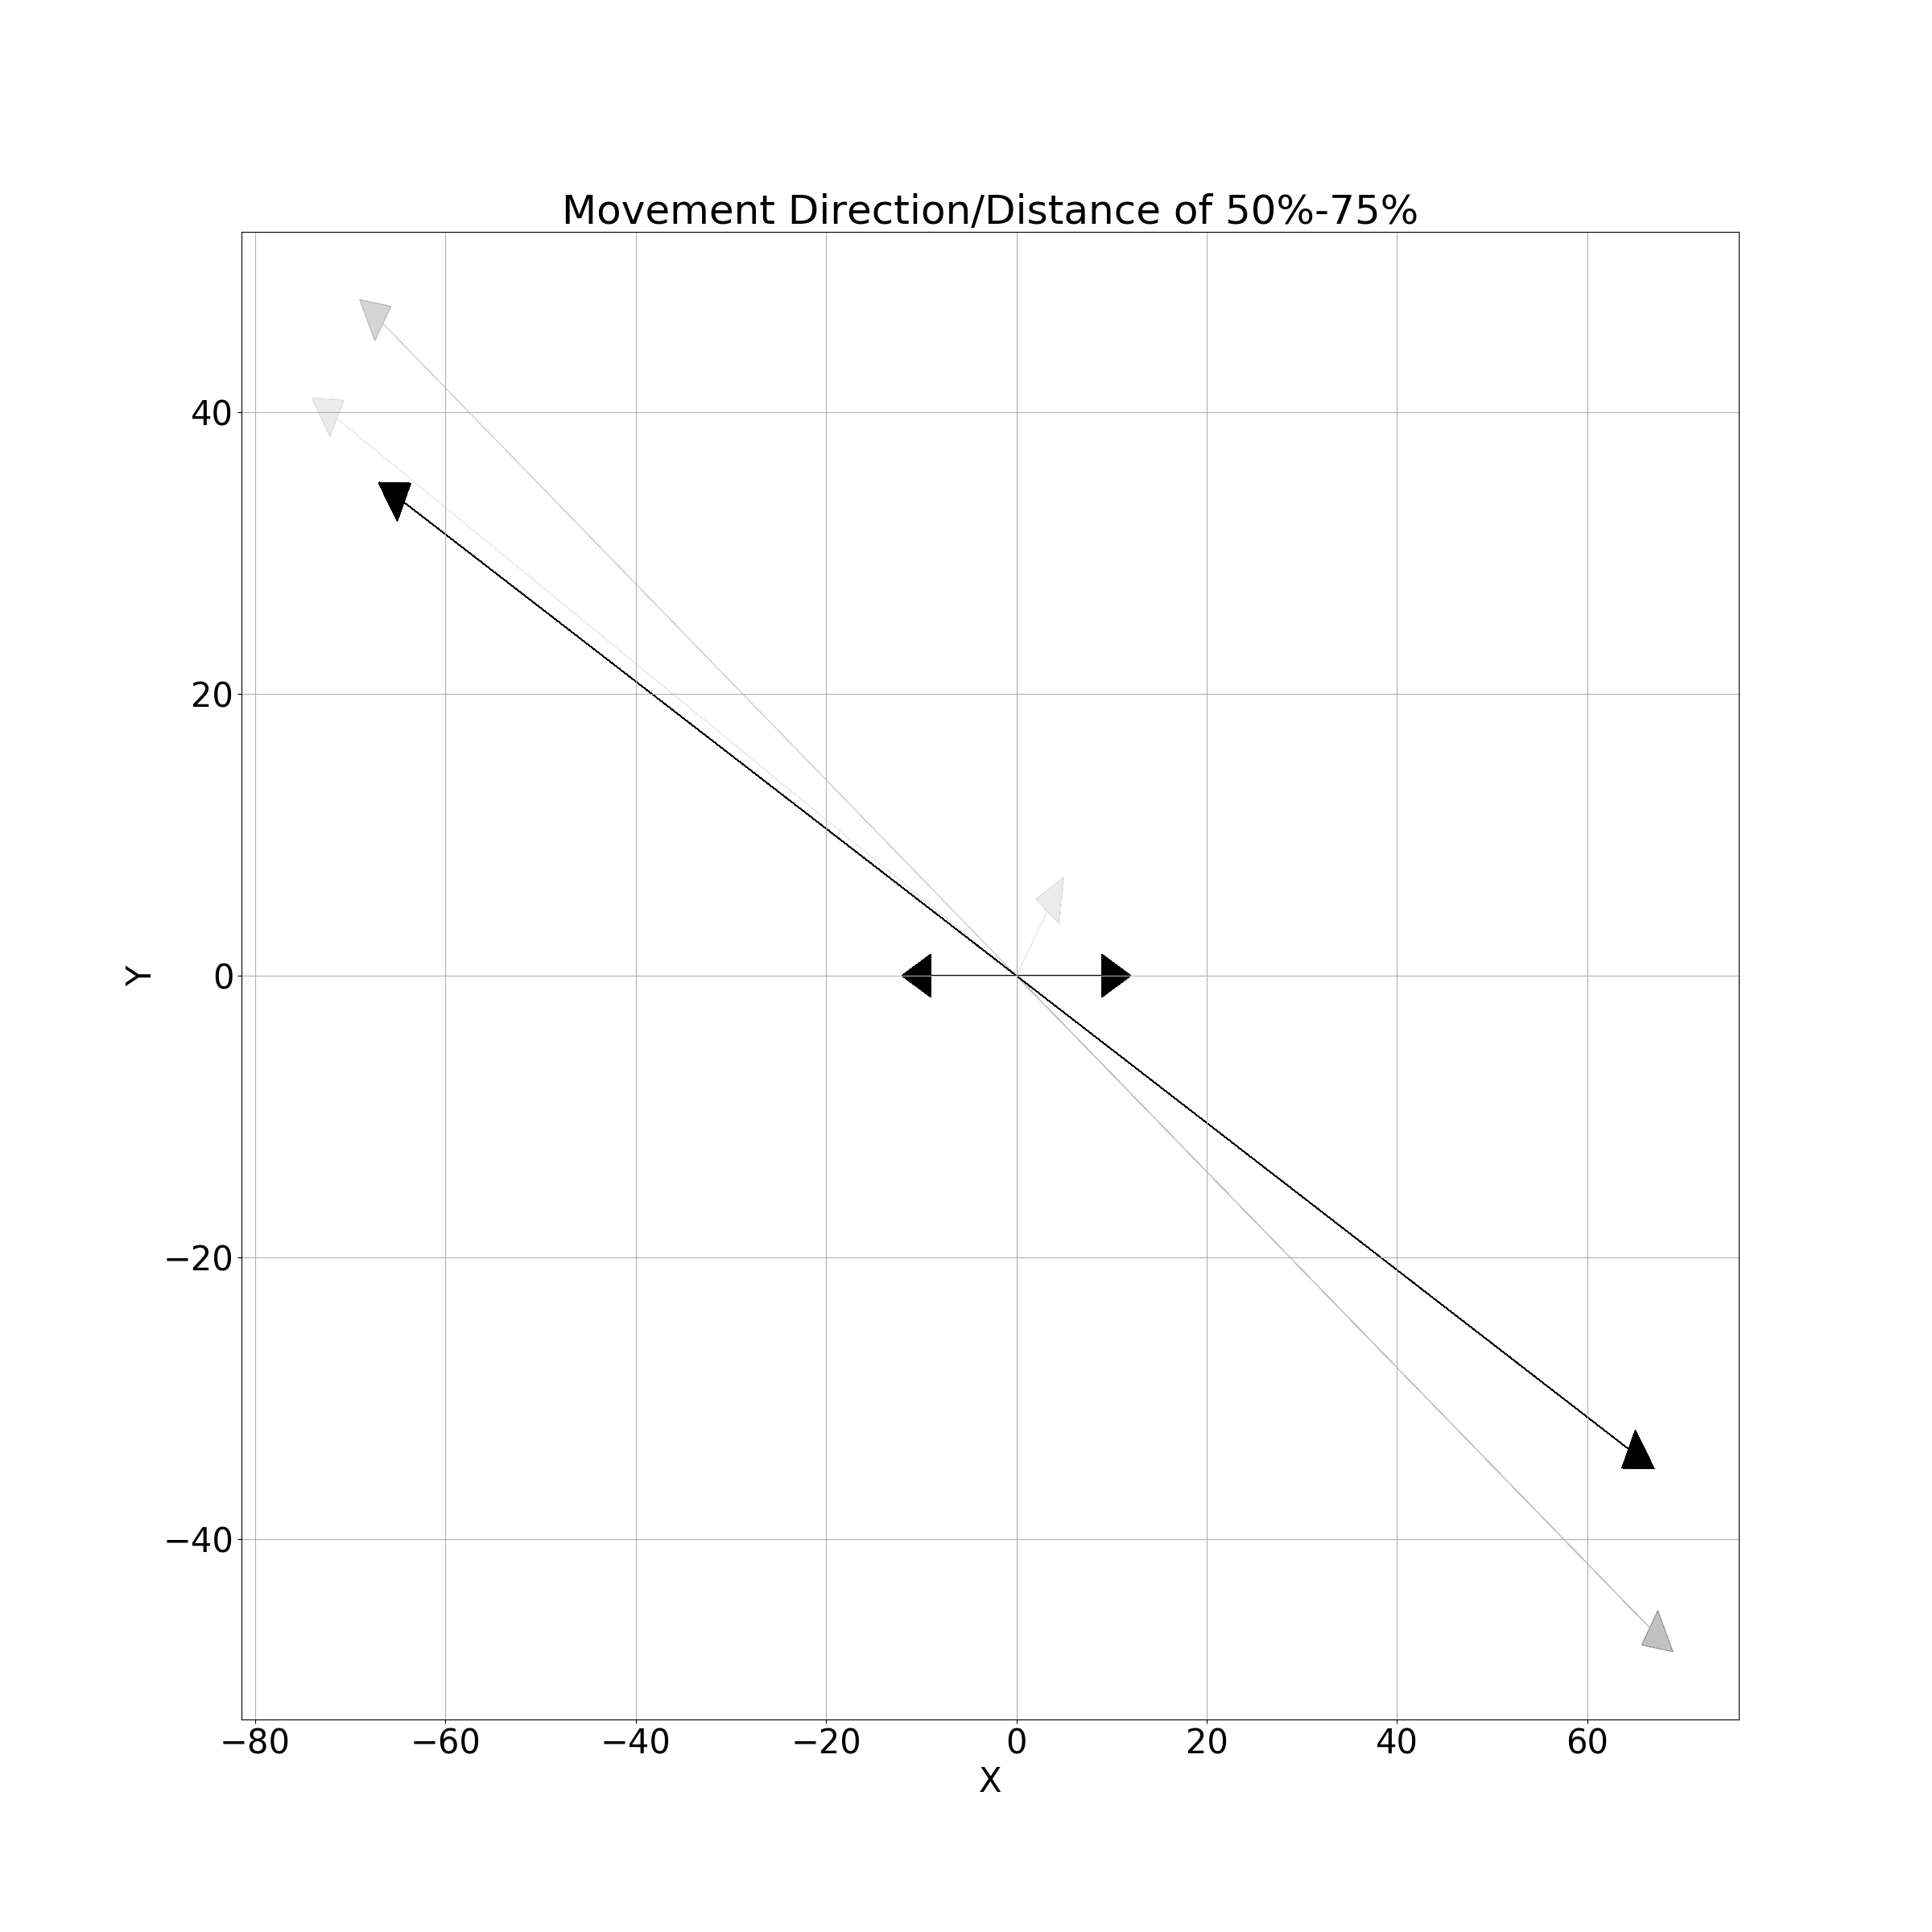
\includegraphics[width=0.3 \linewidth]{figures/movement1-3.png}
                        &
                        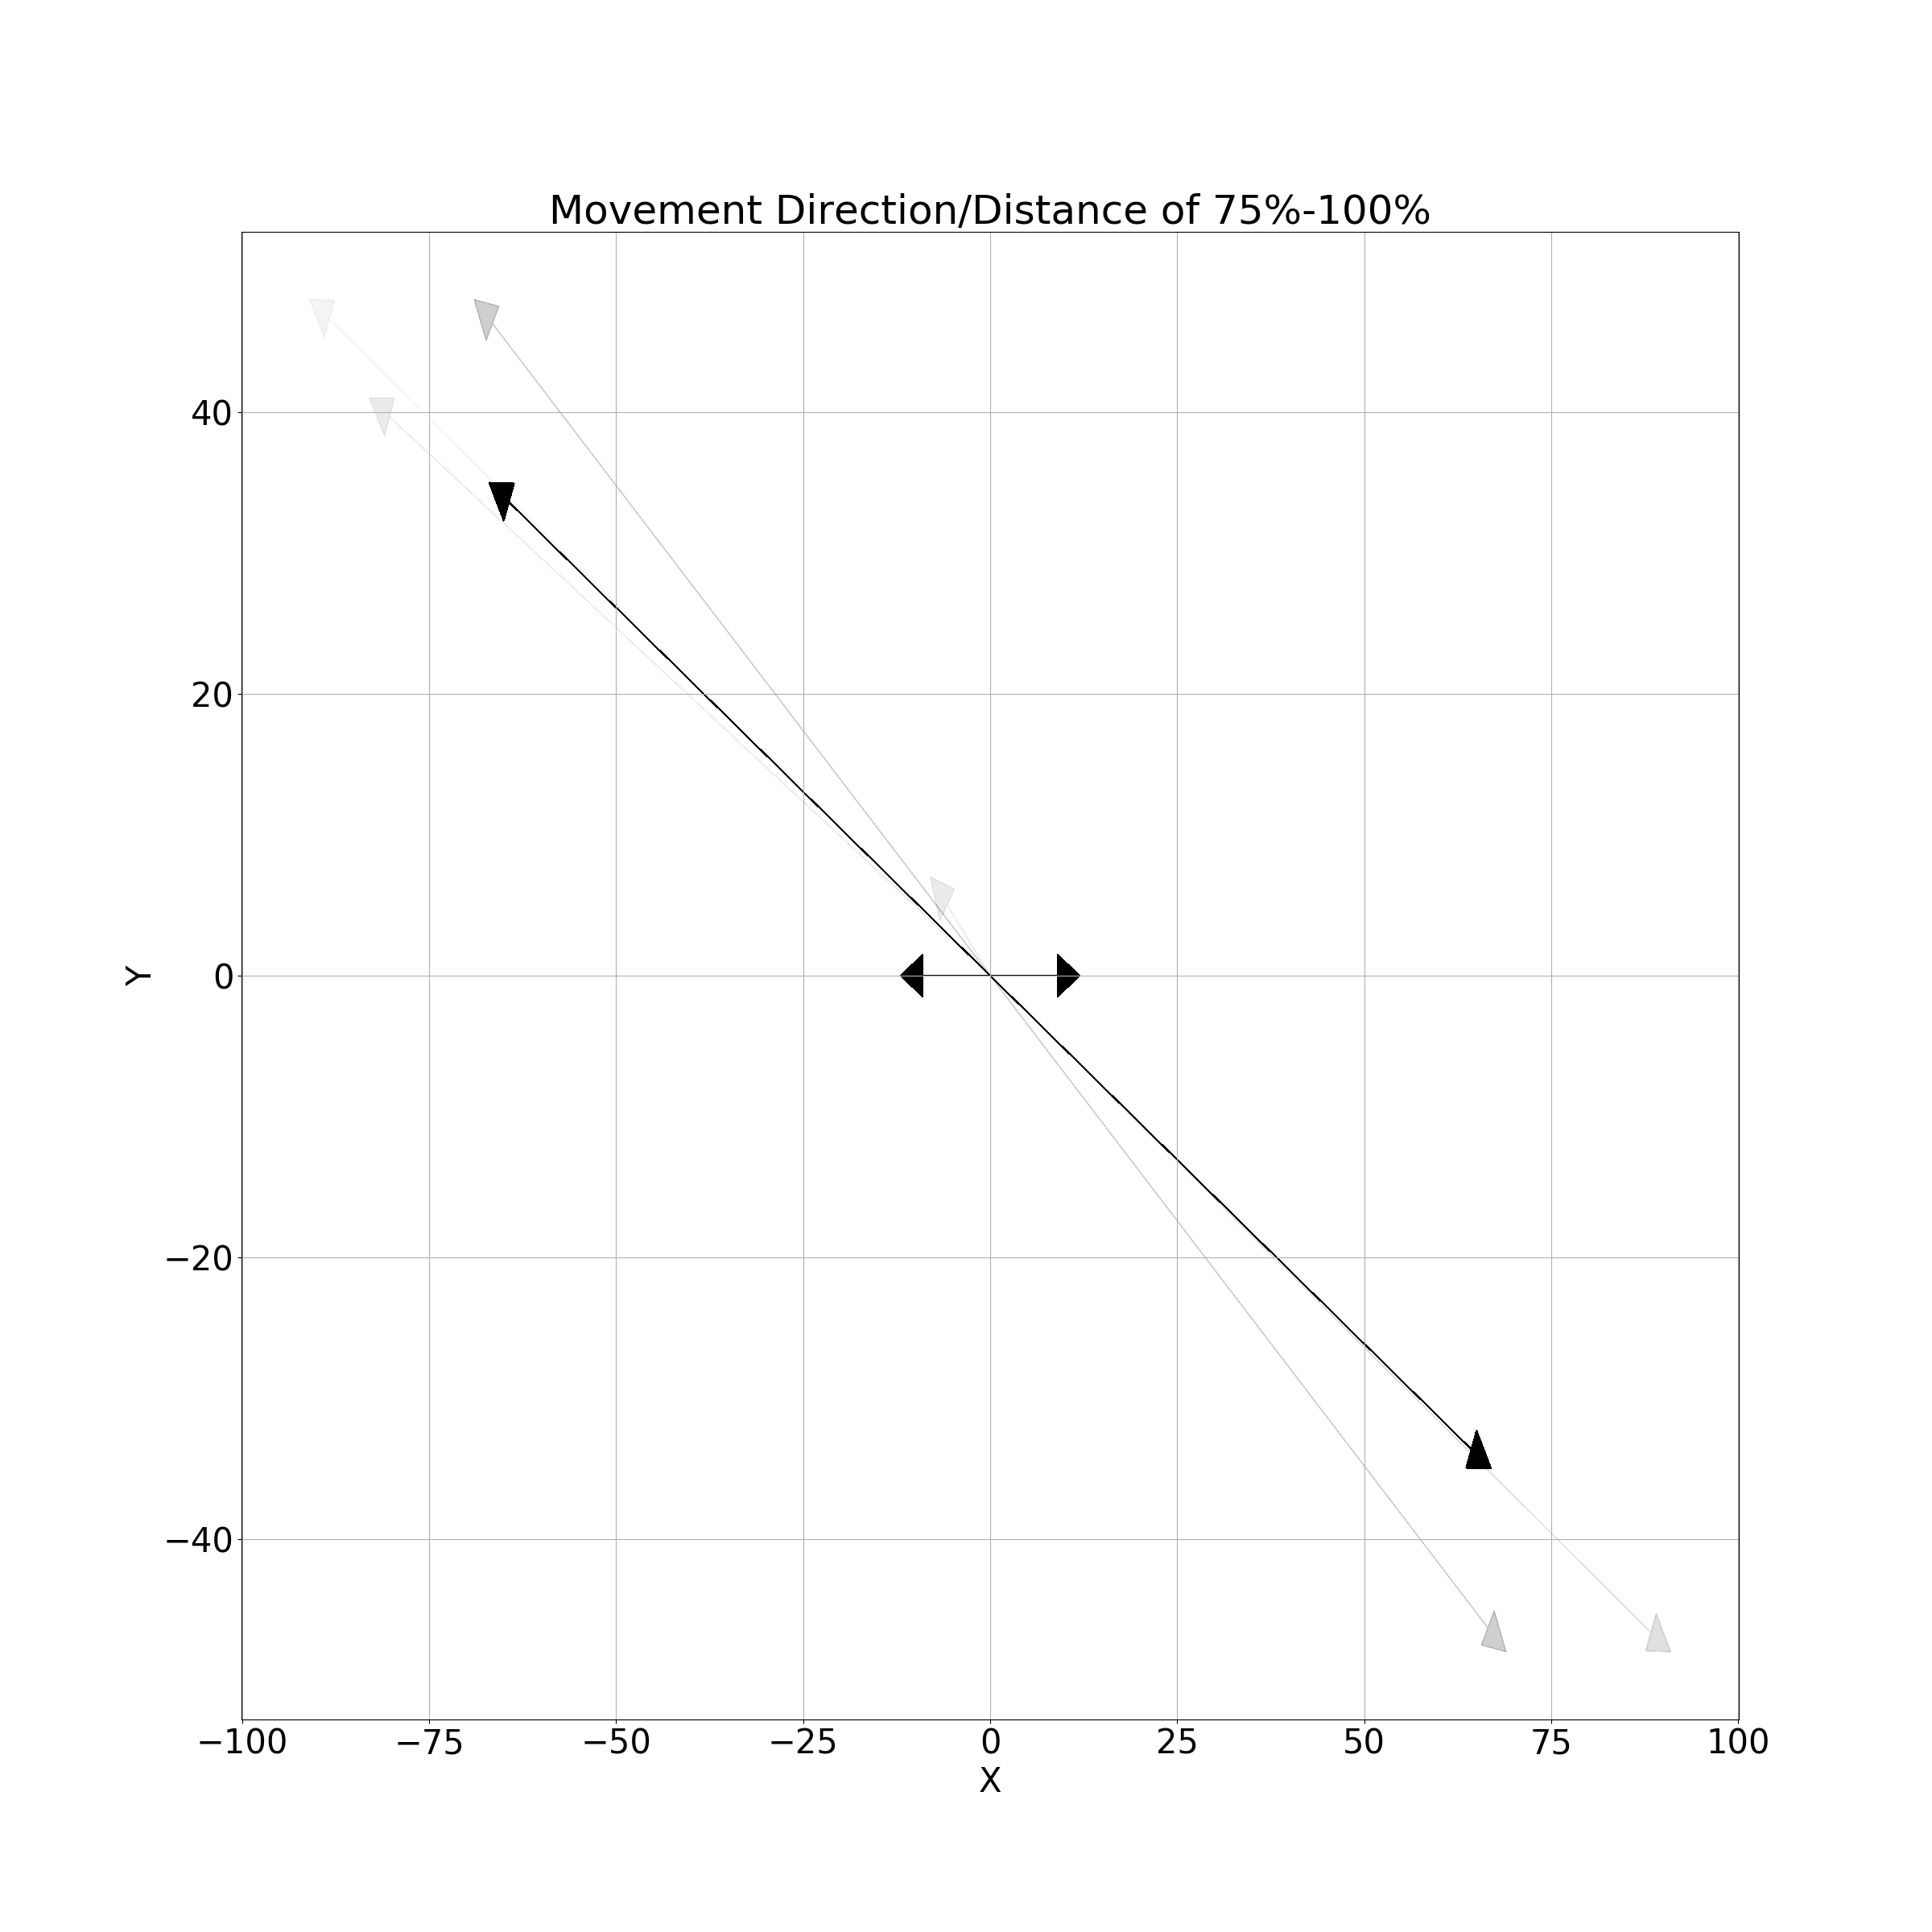
\includegraphics[width=0.3 \linewidth]{figures/movement1-4.png}
                        \\
                        
                        \mbox{(c) 50\%-75\%} & \mbox{(d) 75\%-100\%} \\
                    \end{array}$
                    \caption{Movement Direction/Distance on First Floor}
                    \label{fig:movedd1}
                \end{figure}
            
                The movement direction and distance on the first floor is shows as figure \ref{fig:movedd1}. In figure \ref{fig:movedd1}-(b, c, d), you can see two arrows: one is left-upward arrow, the other is right-downward arrow. 
                
                \begin{figure}[htbp]
                    \centering
                    $\begin{array}{cc}
                    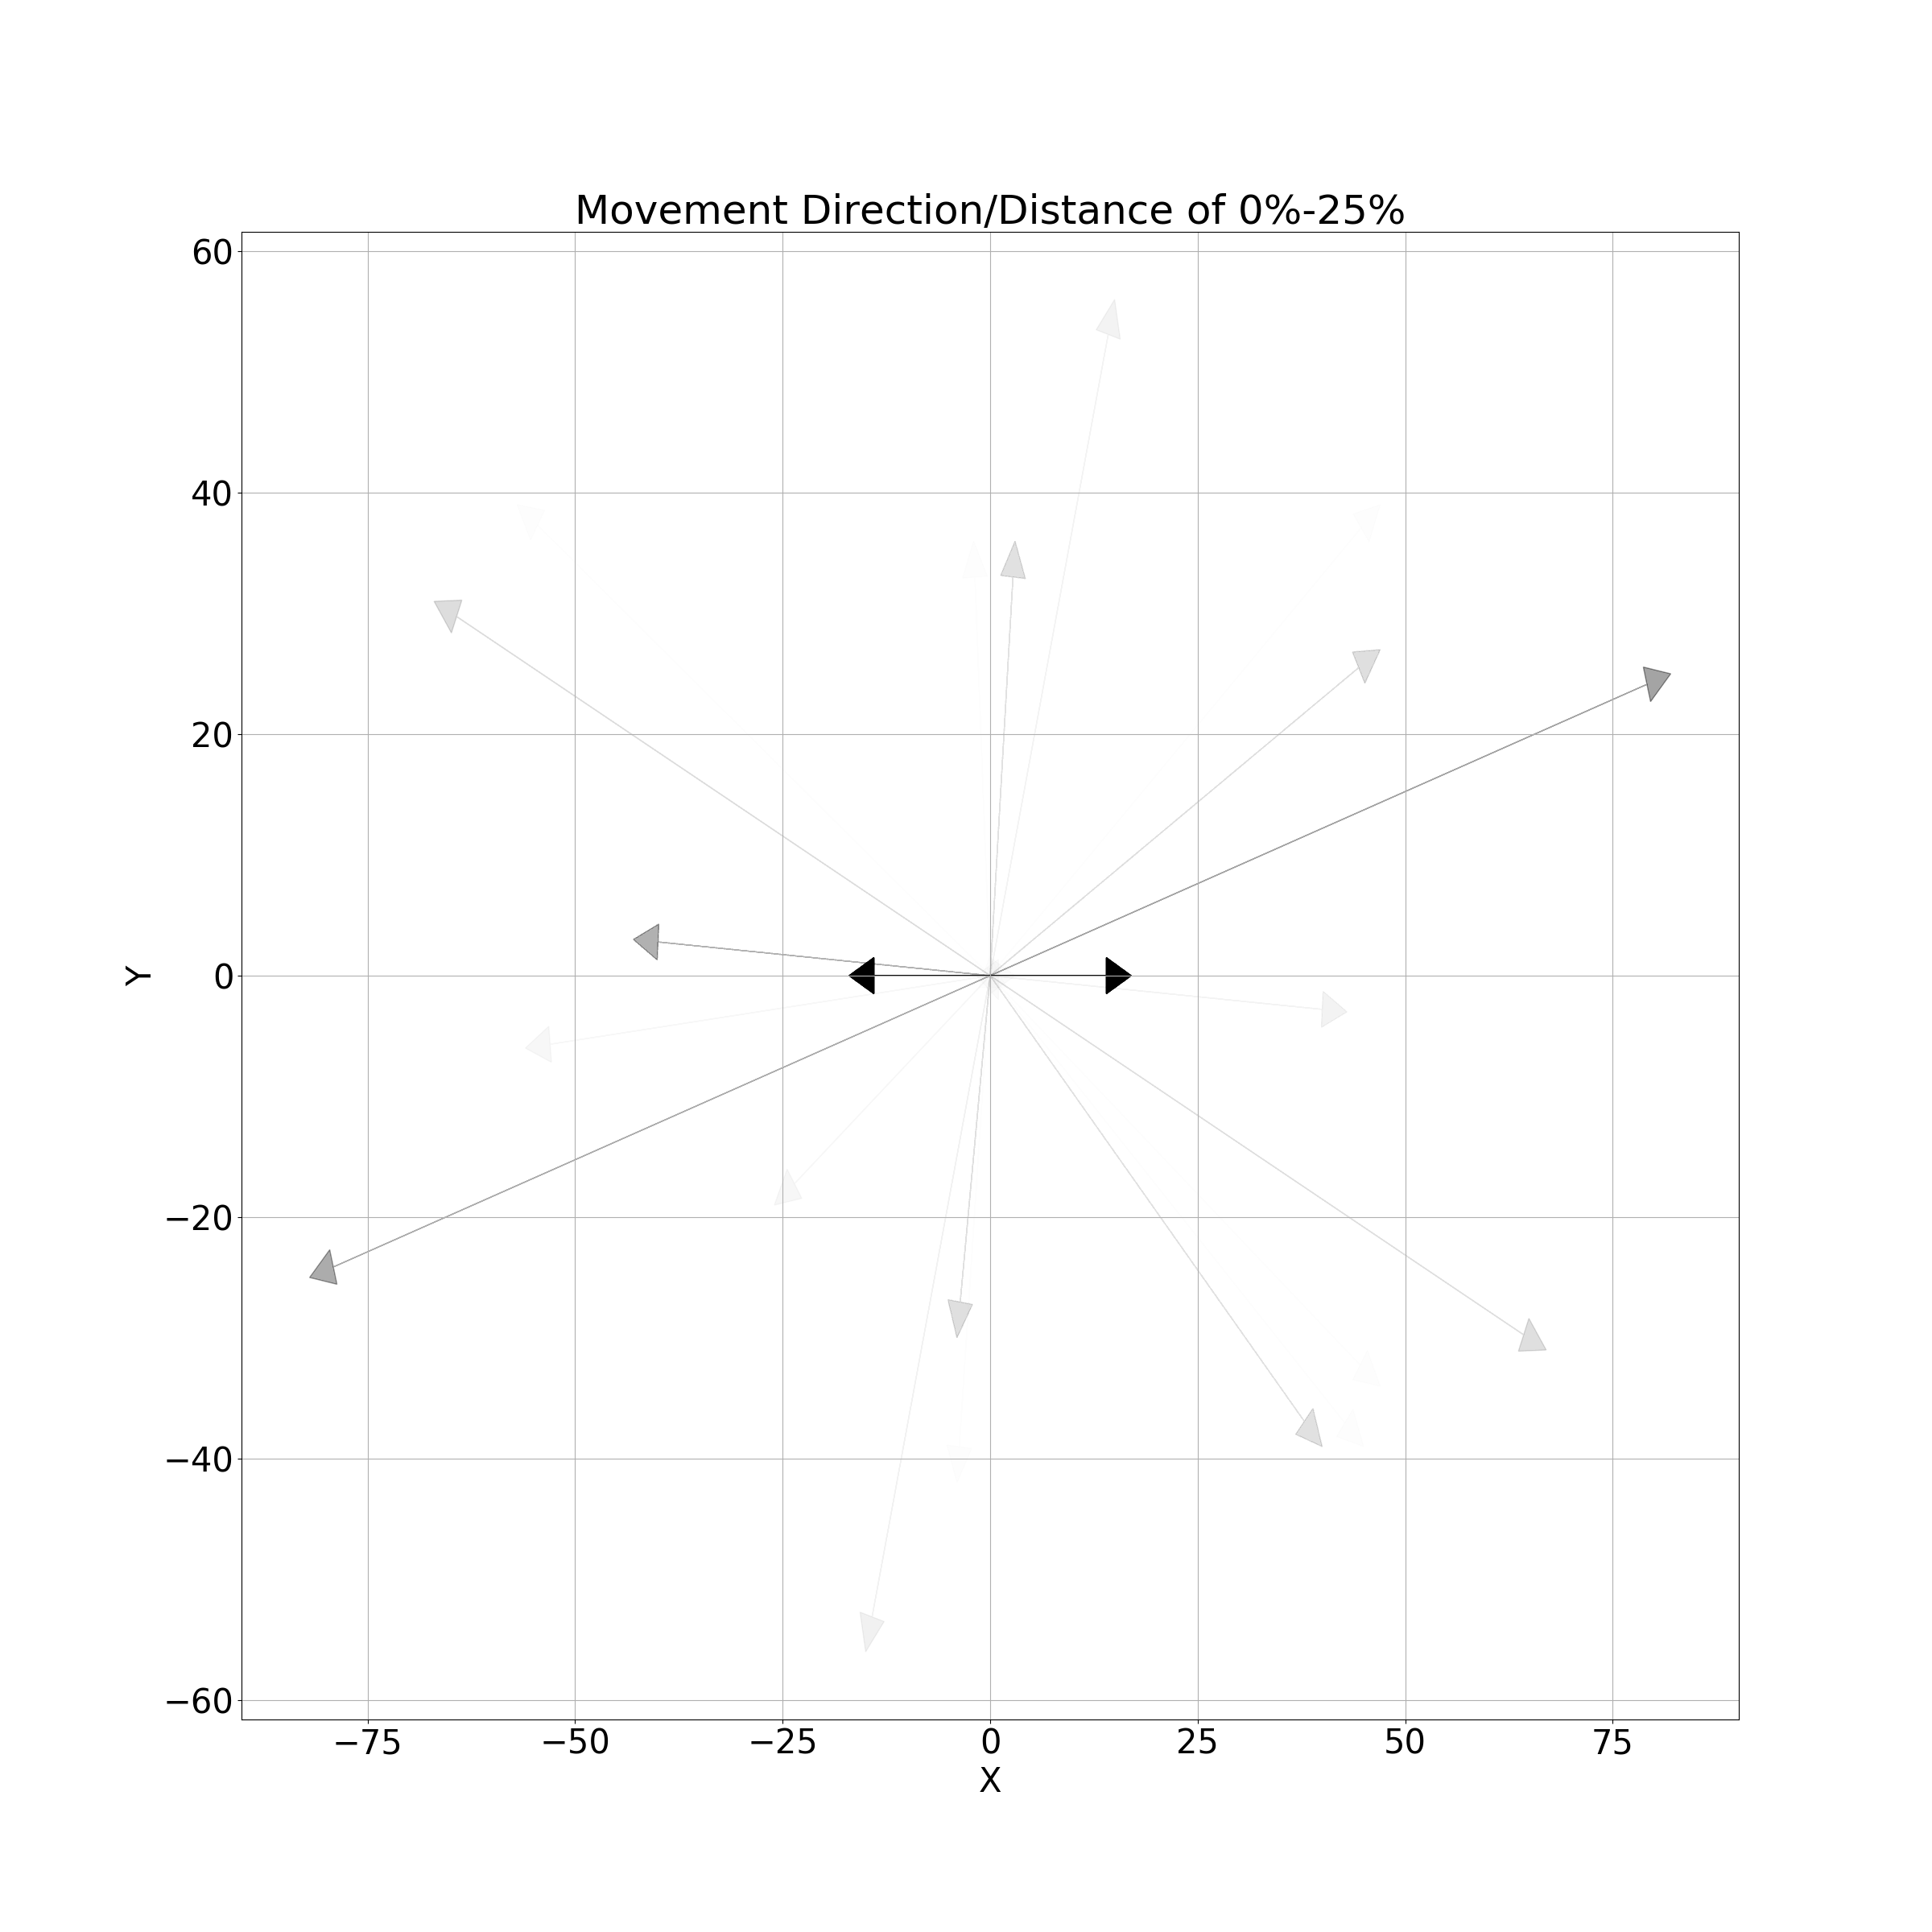
\includegraphics[width=0.3 \linewidth]{figures/movement2-1.png}
                    &
                    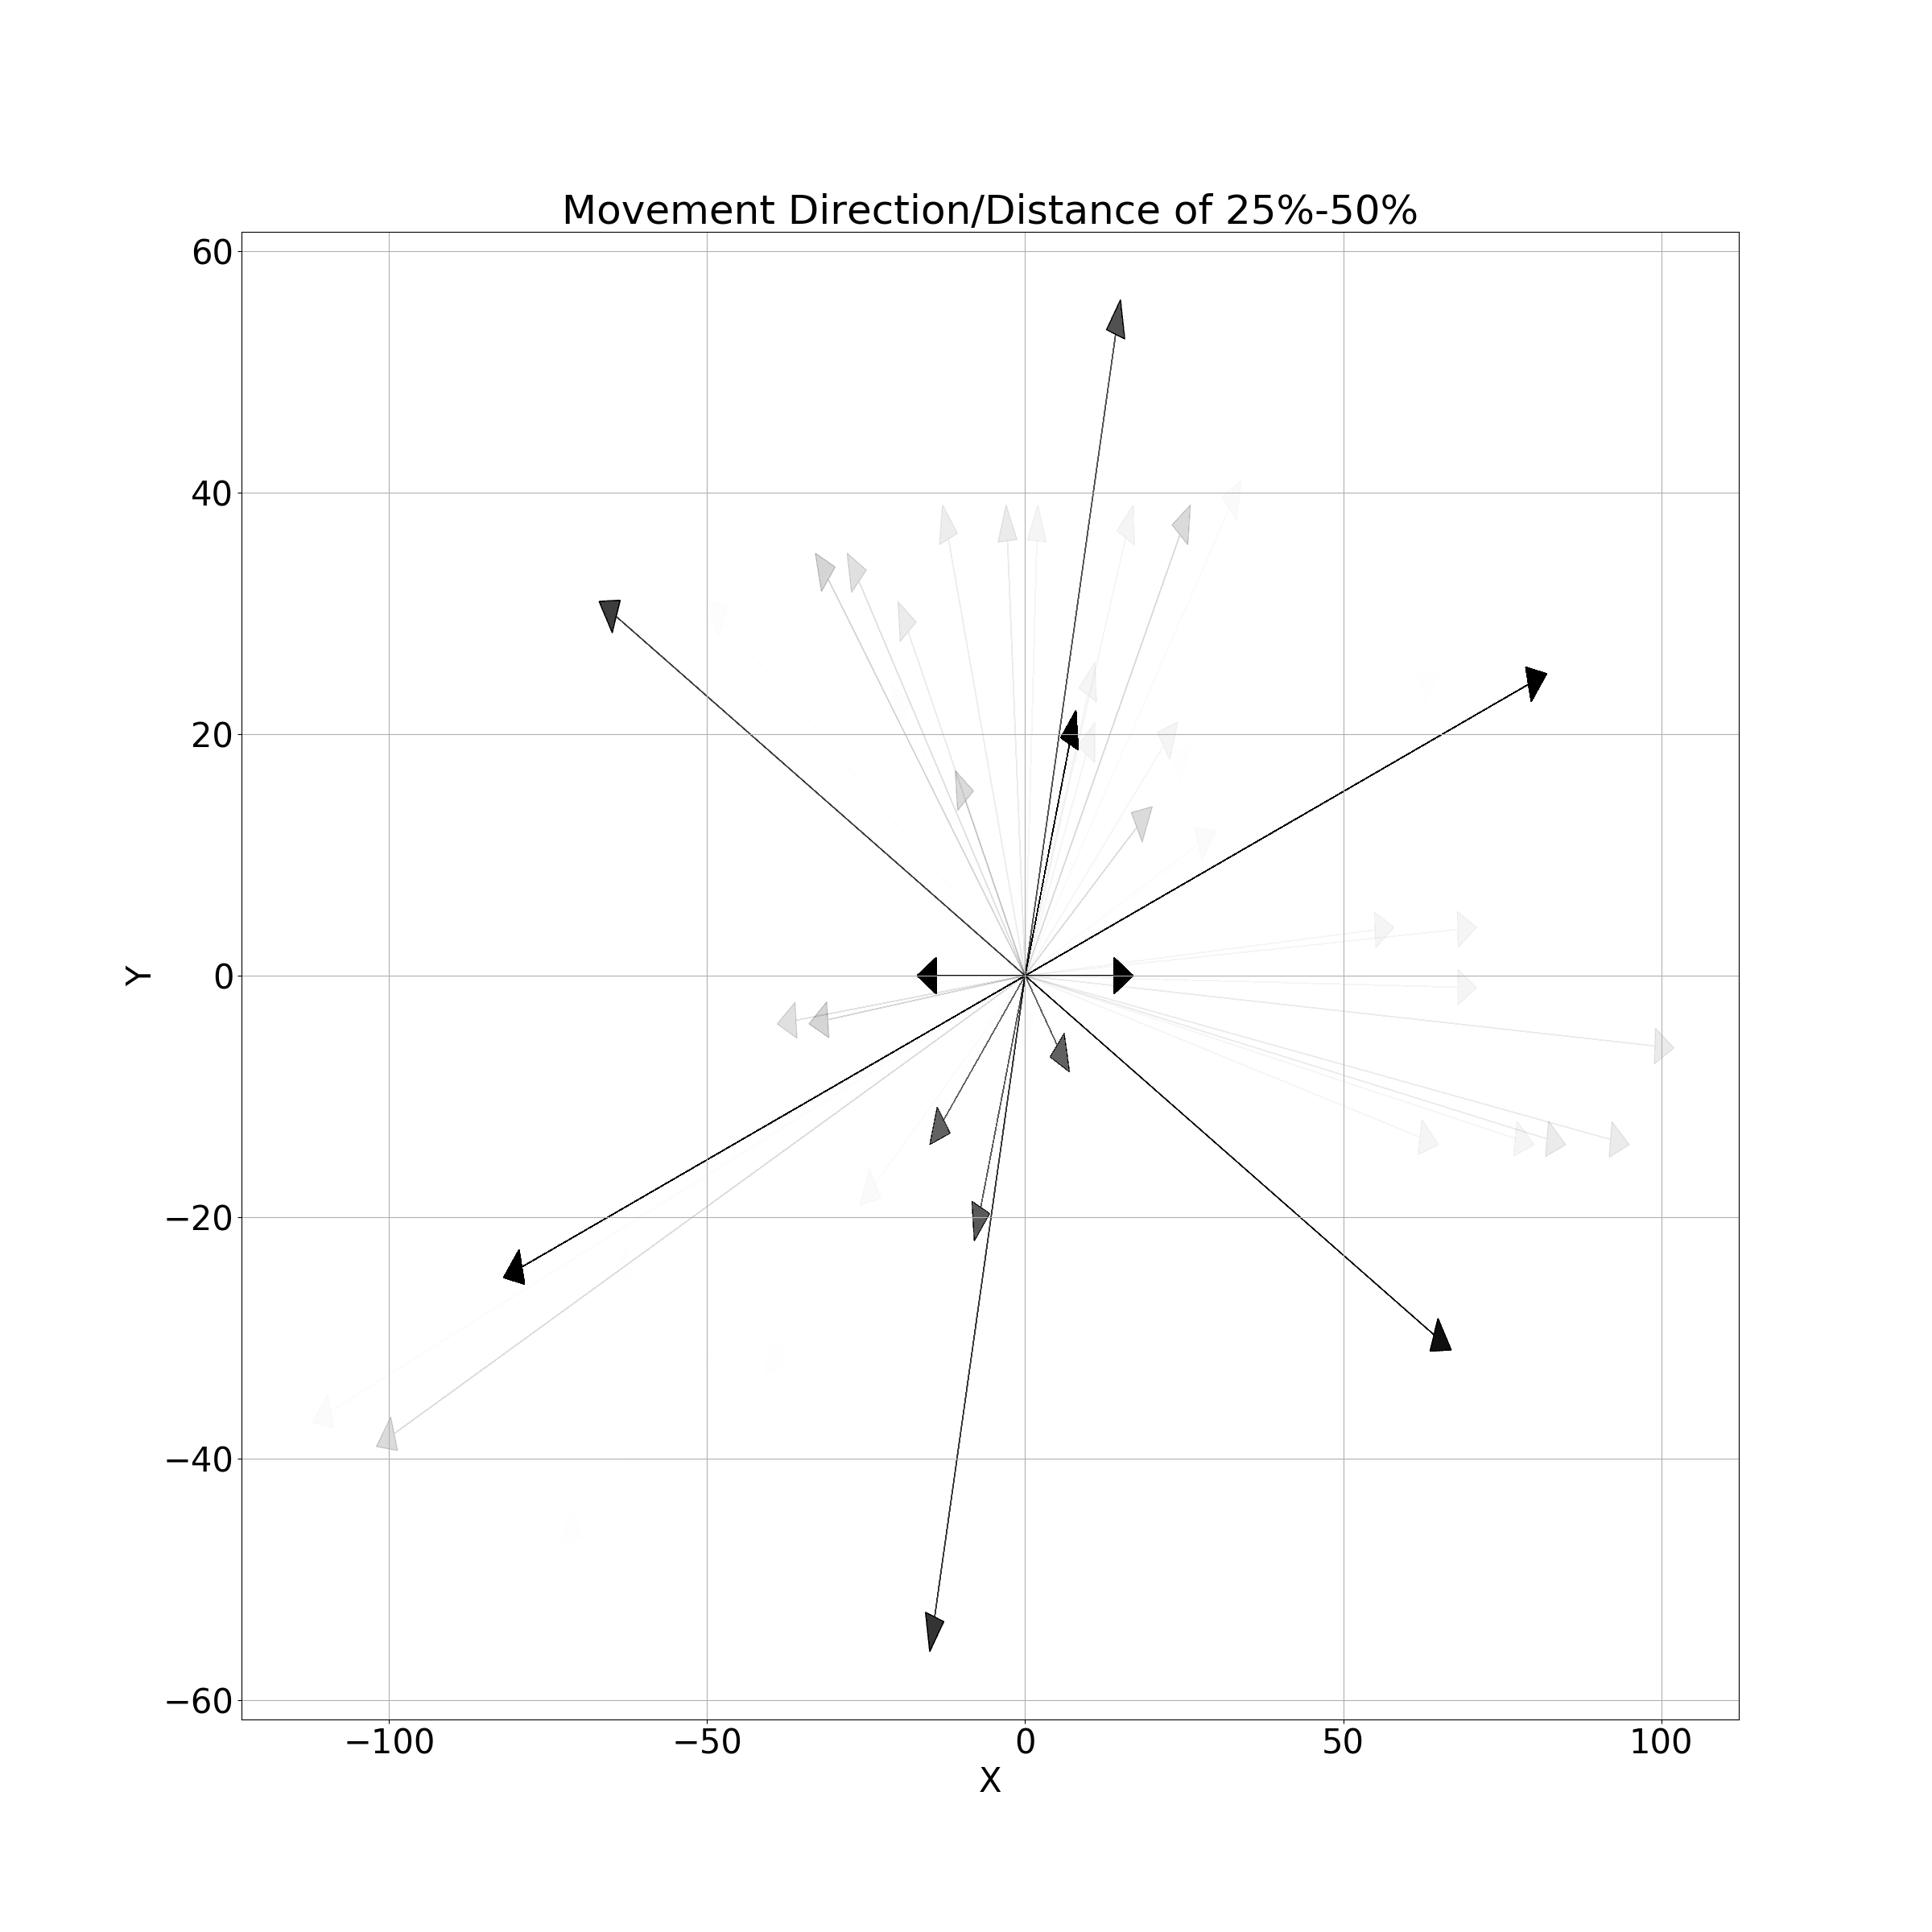
\includegraphics[width=0.3 \linewidth]{figures/movement2-2.png}
                    \\
                    
                    \mbox{(a) 0\%-25\%} & \mbox{(b) 25\%-50\%} \\
                    
                    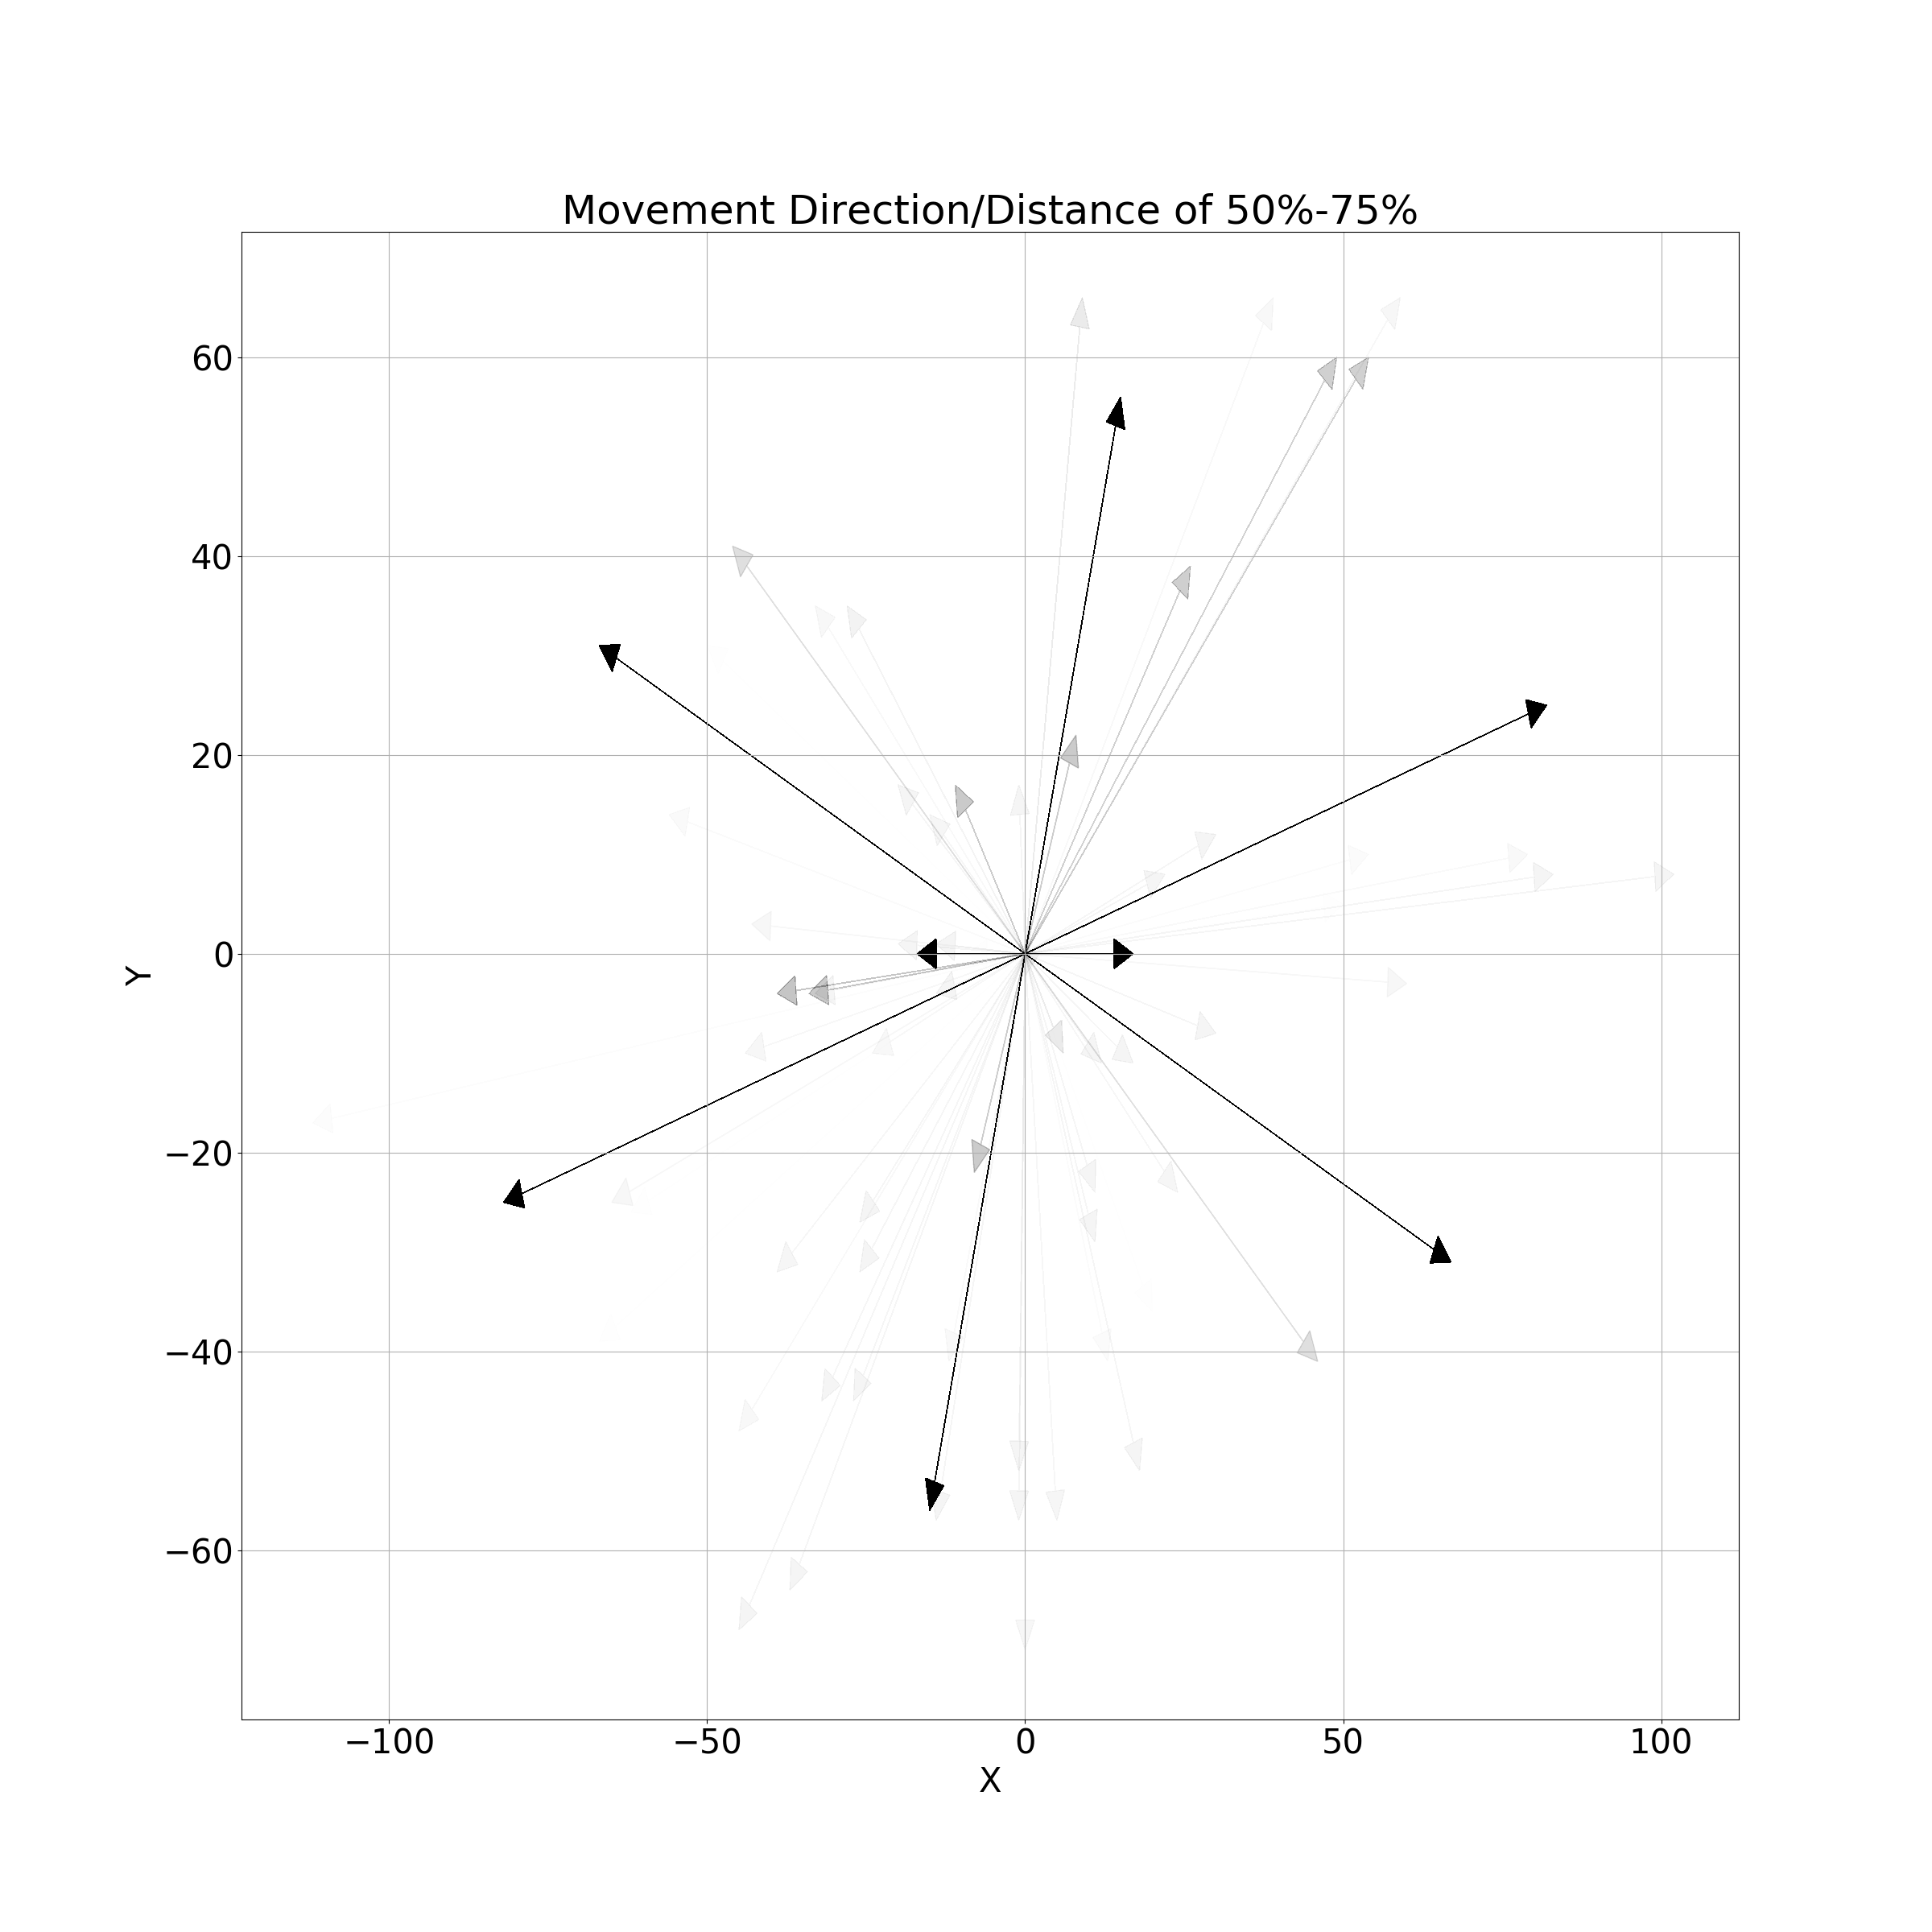
\includegraphics[width=0.3 \linewidth]{figures/movement2-3.png}
                    &
                    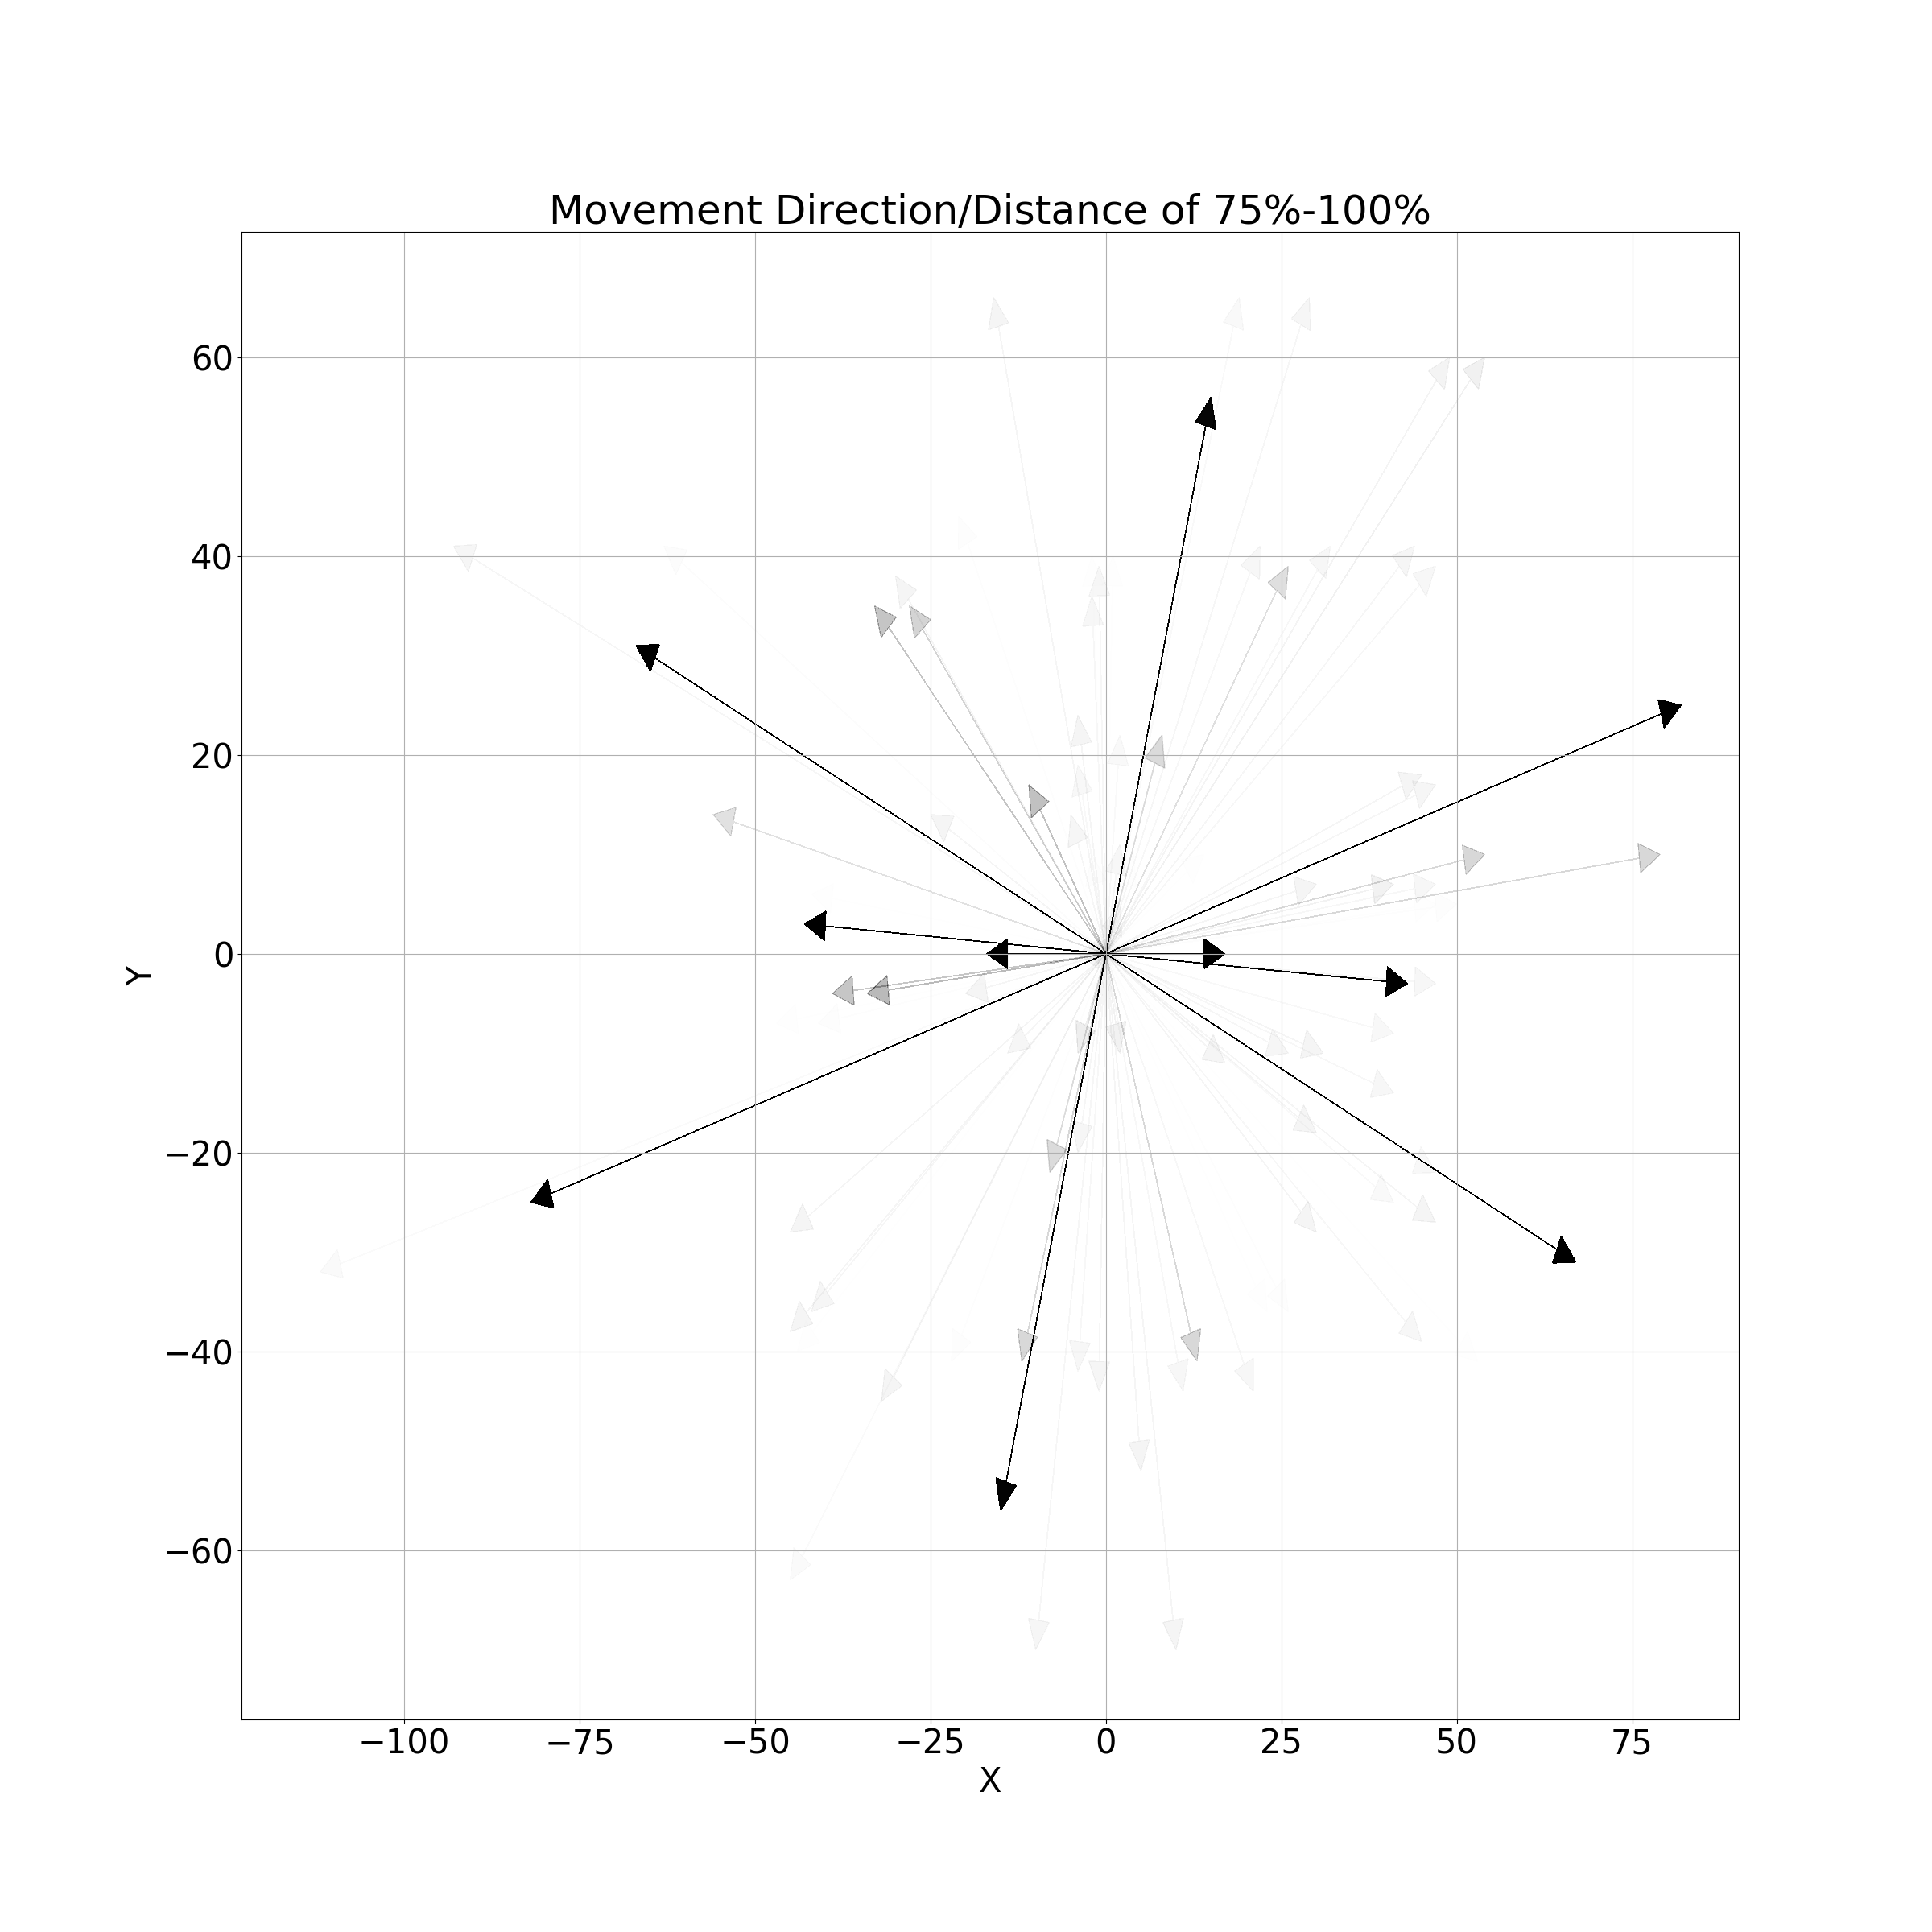
\includegraphics[width=0.3 \linewidth]{figures/movement2-4.png}
                    \\
                    
                    \mbox{(c) 50\%-75\%} & \mbox{(d) 75\%-100\%} \\
                \end{array}$
                \caption{Movement Direction/Distance on Second Floor}
                \label{fig:movedd2}
                \end{figure}
            
                \begin{figure}[htbp]
                    \centering
                    $\begin{array}{cc}
                    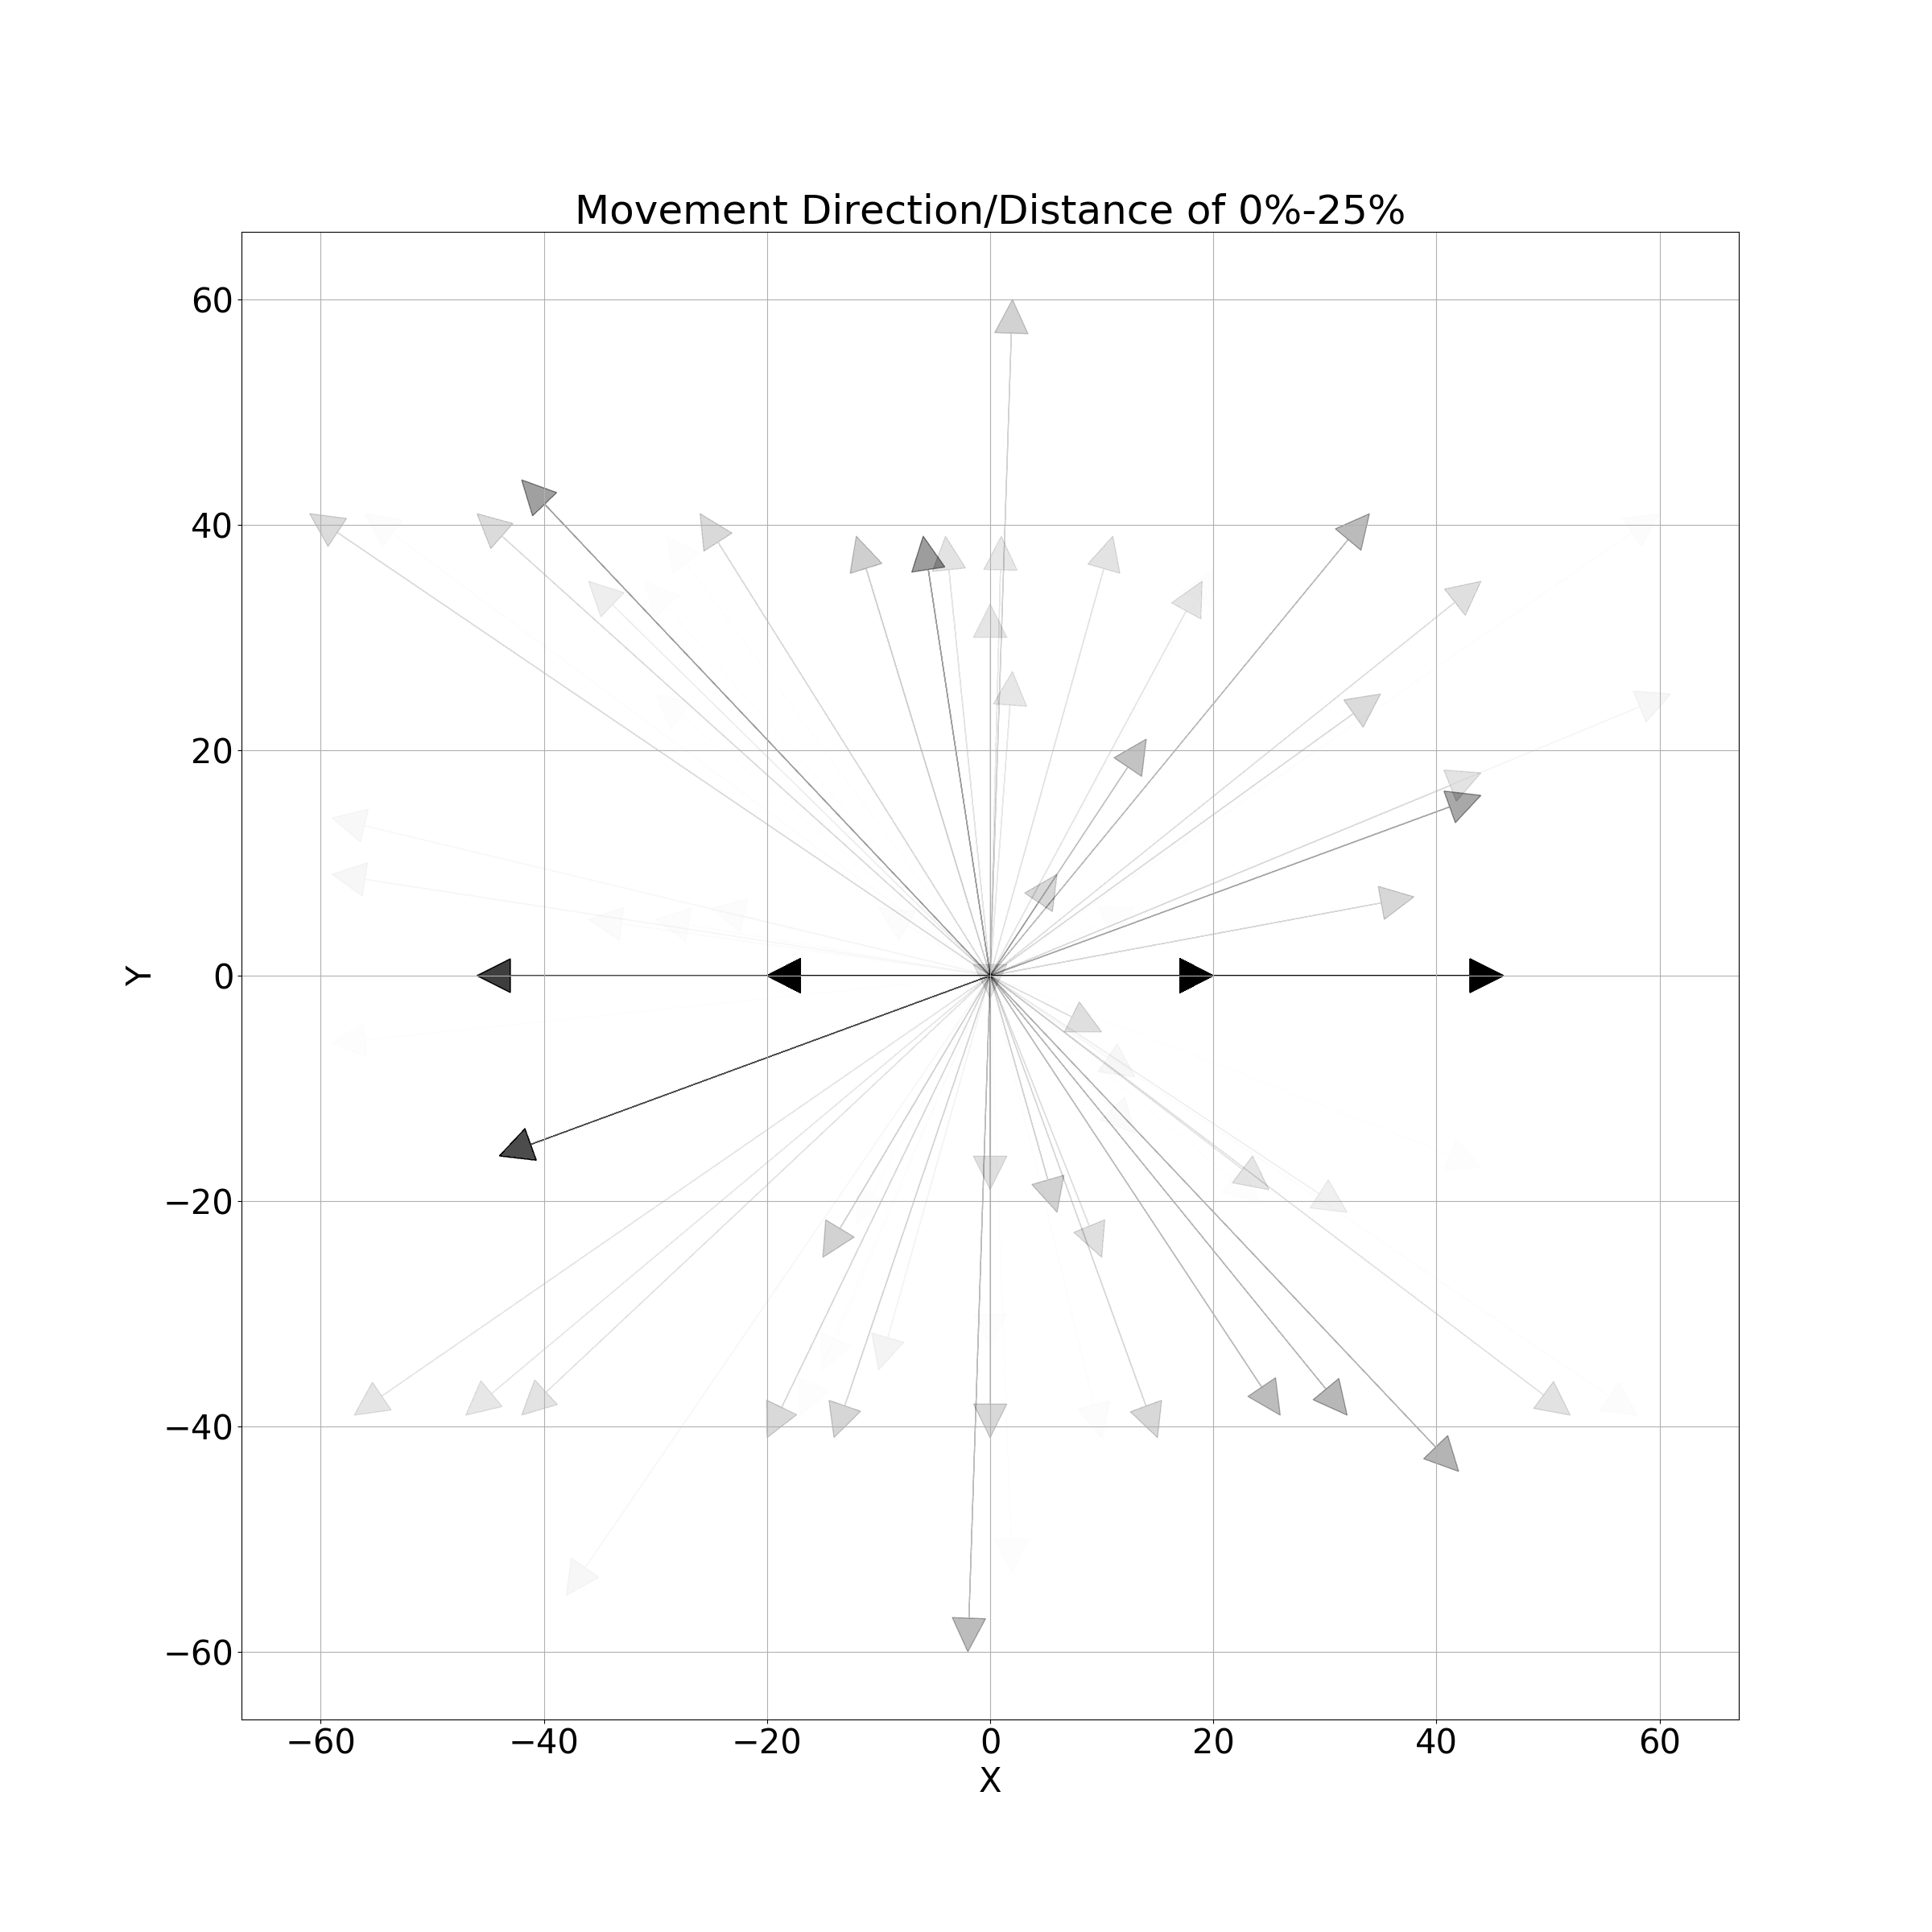
\includegraphics[width=0.3 \linewidth]{figures/movement3-1.png}
                    &
                    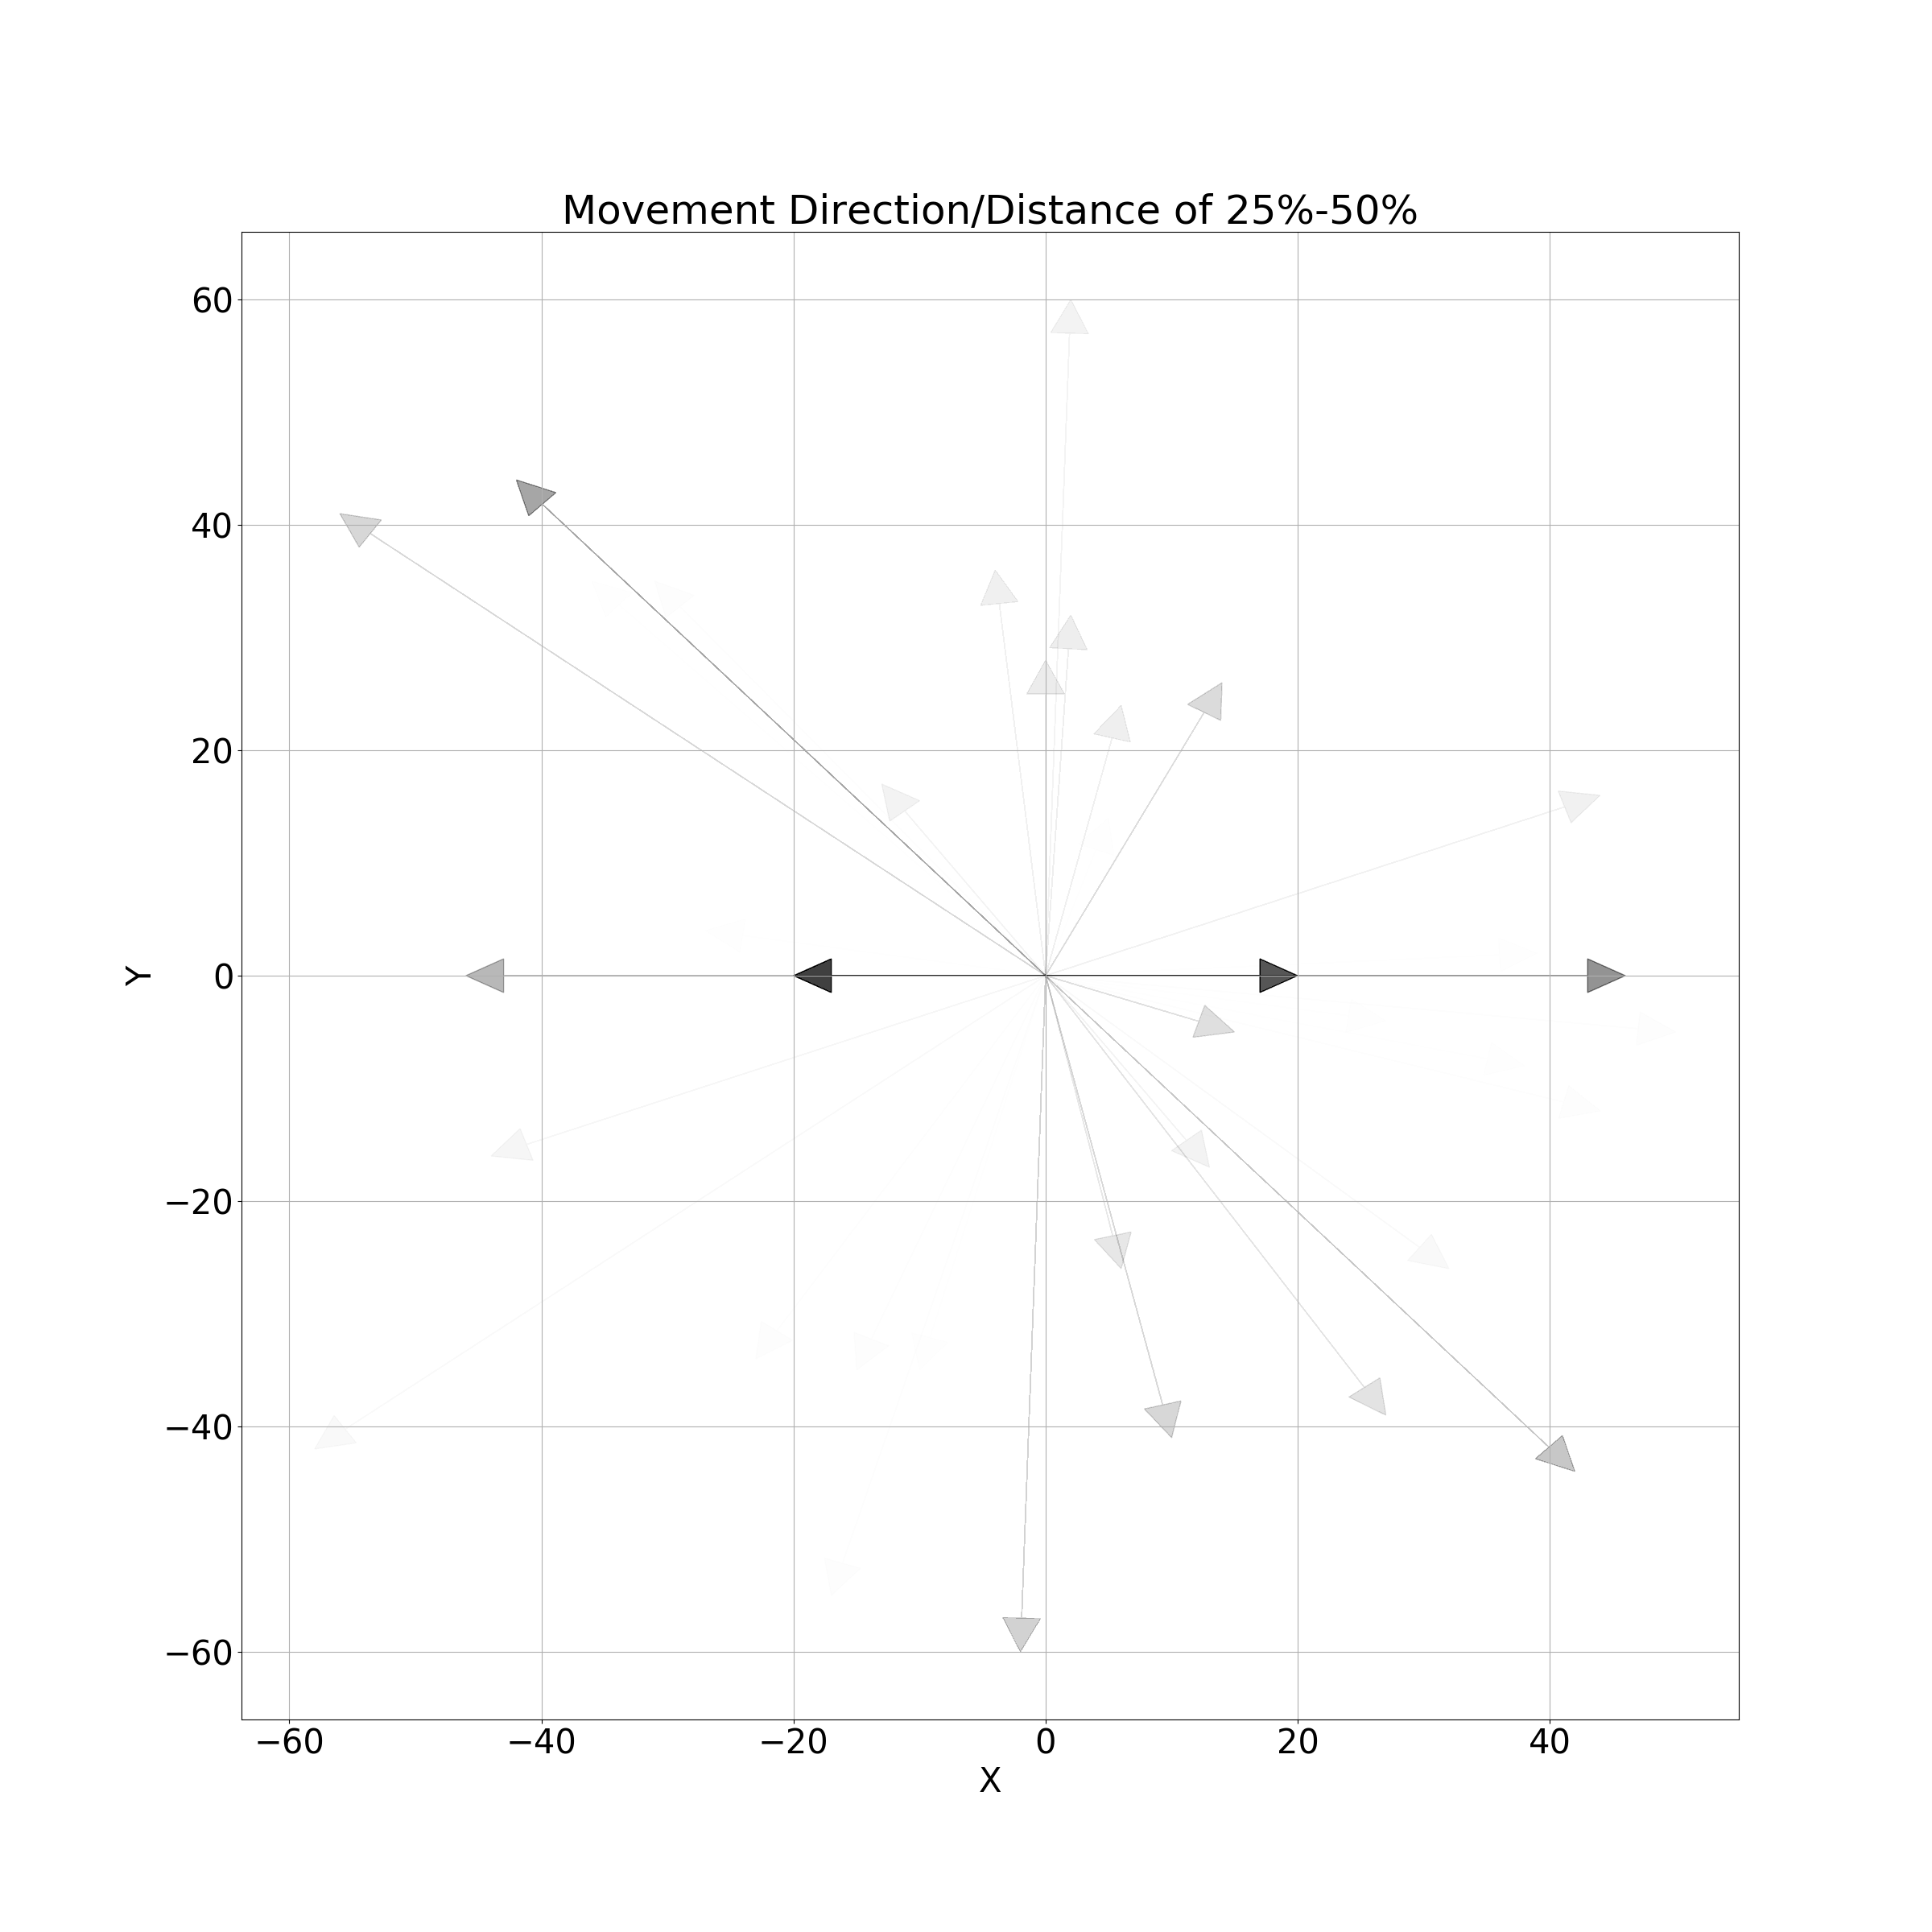
\includegraphics[width=0.3 \linewidth]{figures/movement3-2.png}
                    \\
                    
                    \mbox{(a) 0\%-25\%} & \mbox{(b) 25\%-50\%} \\
                    
                    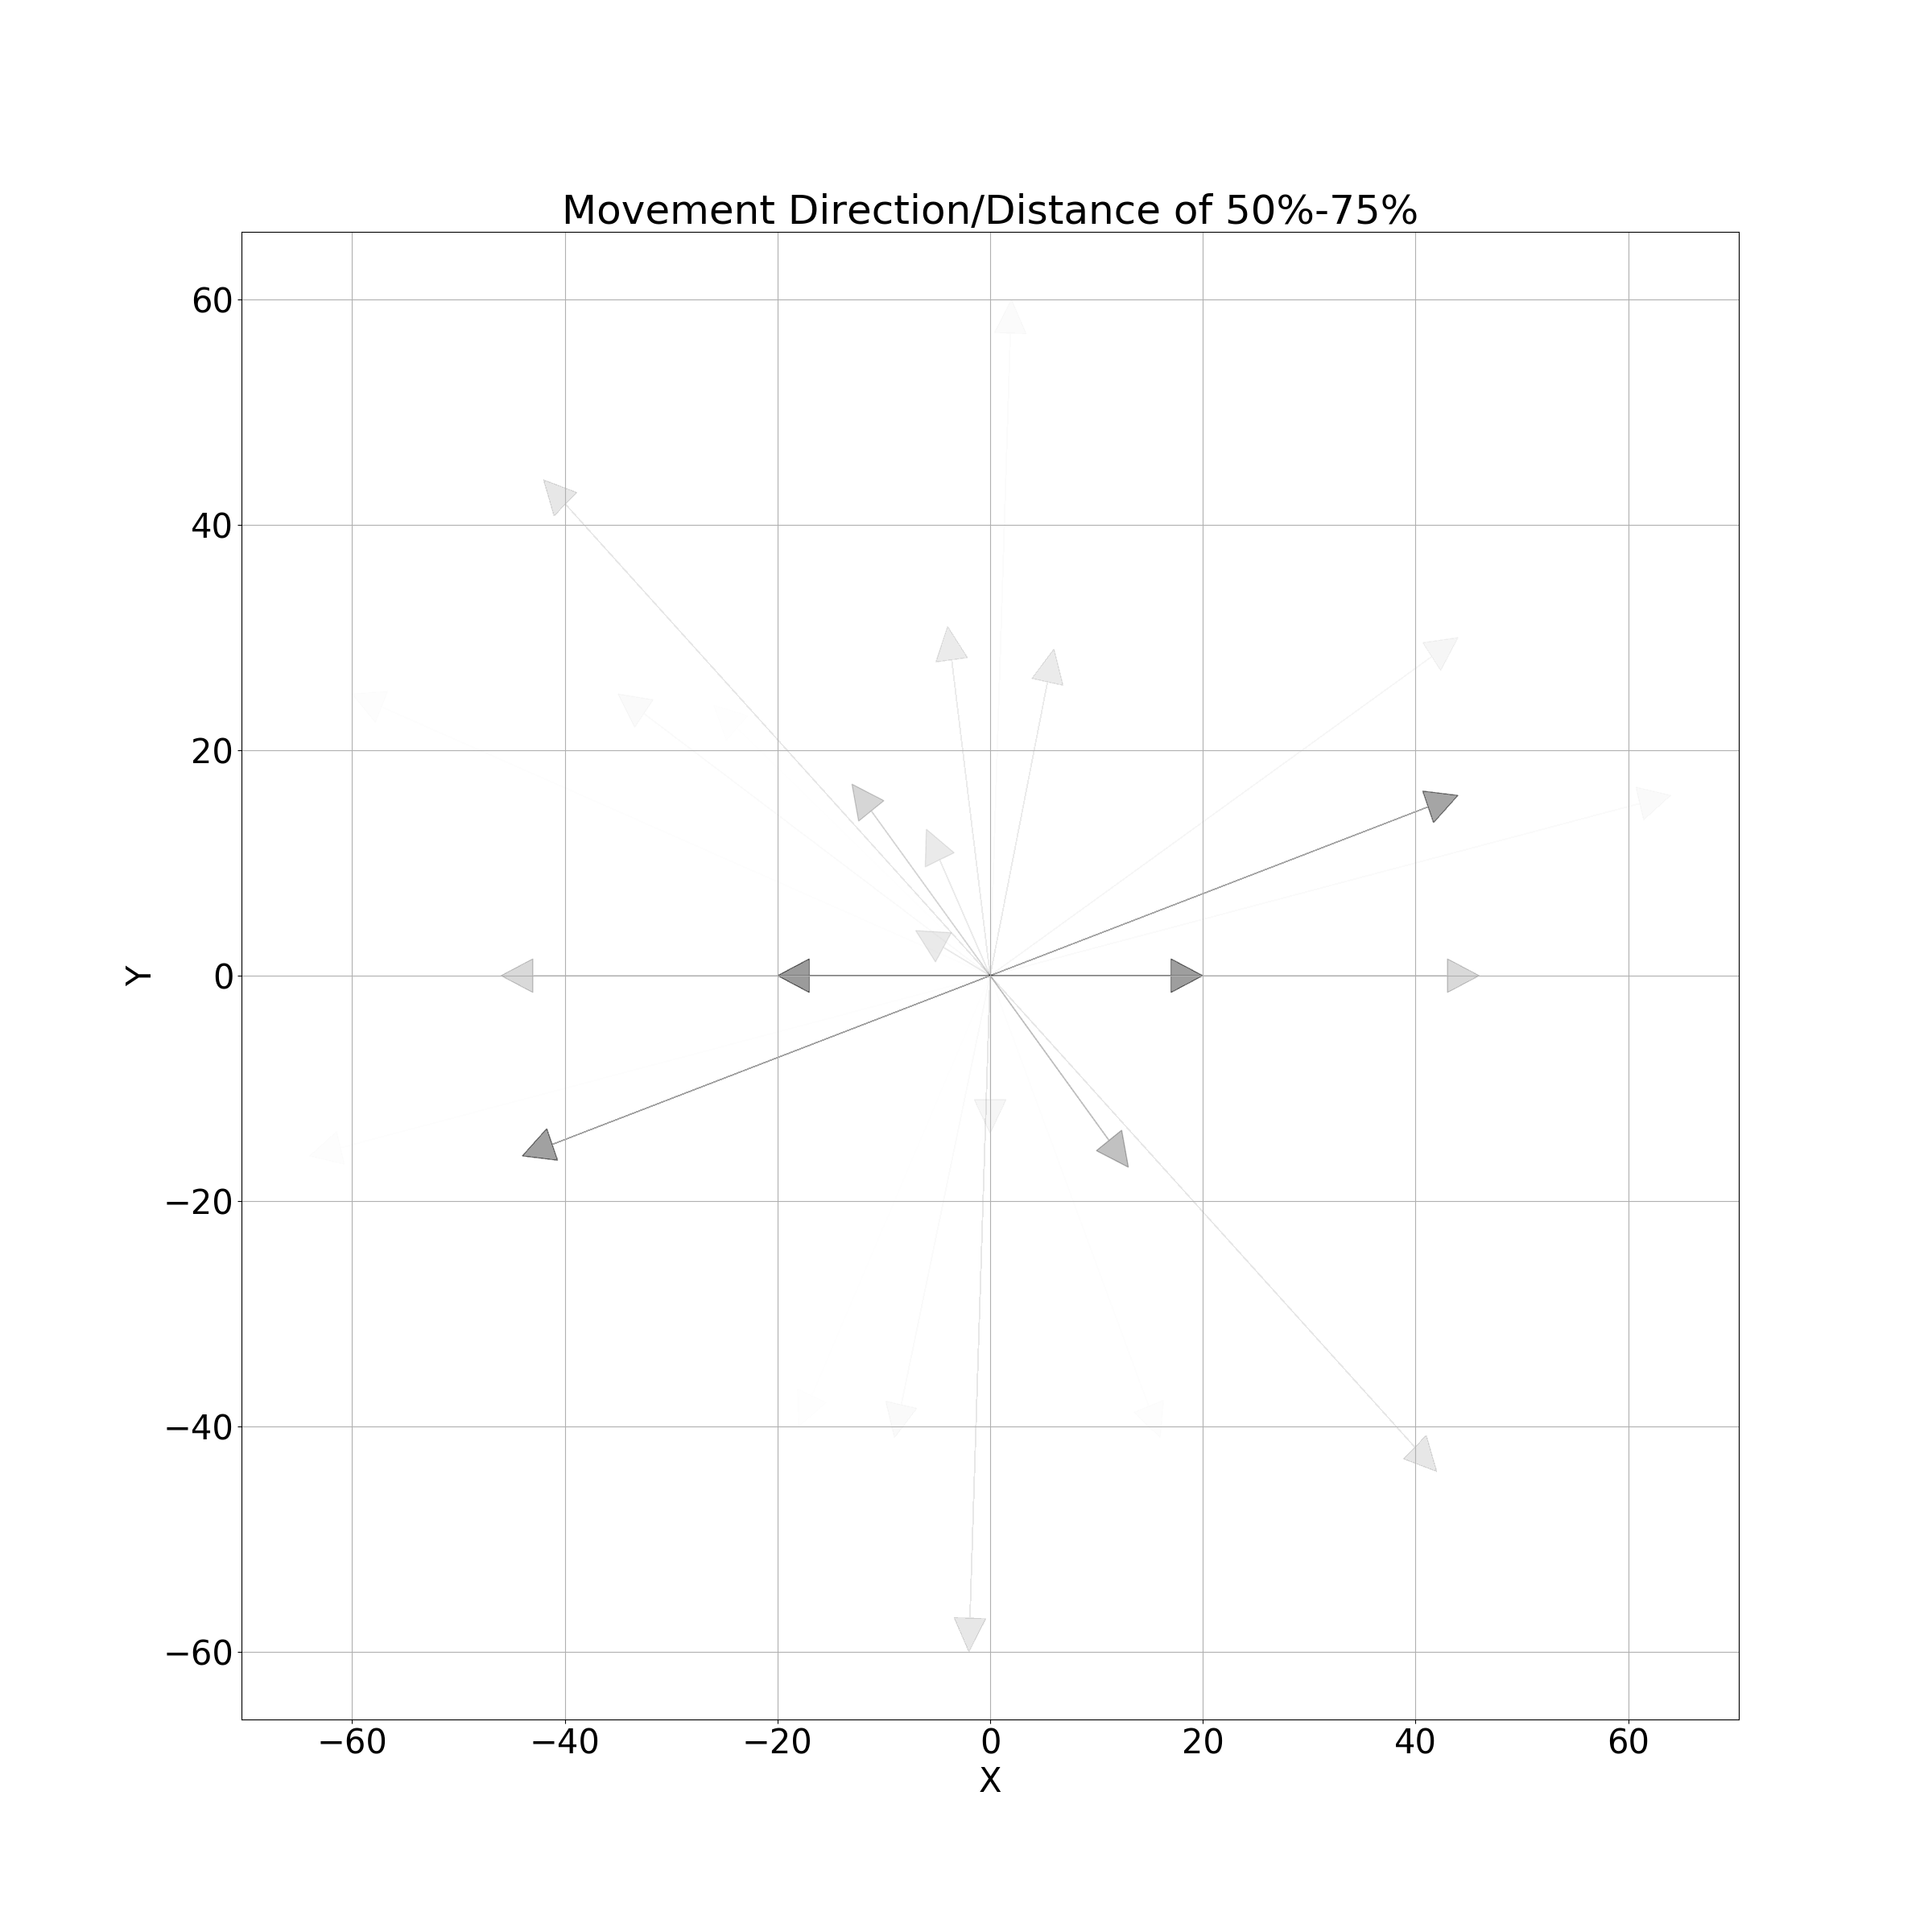
\includegraphics[width=0.3 \linewidth]{figures/movement3-3.png}
                    &
                    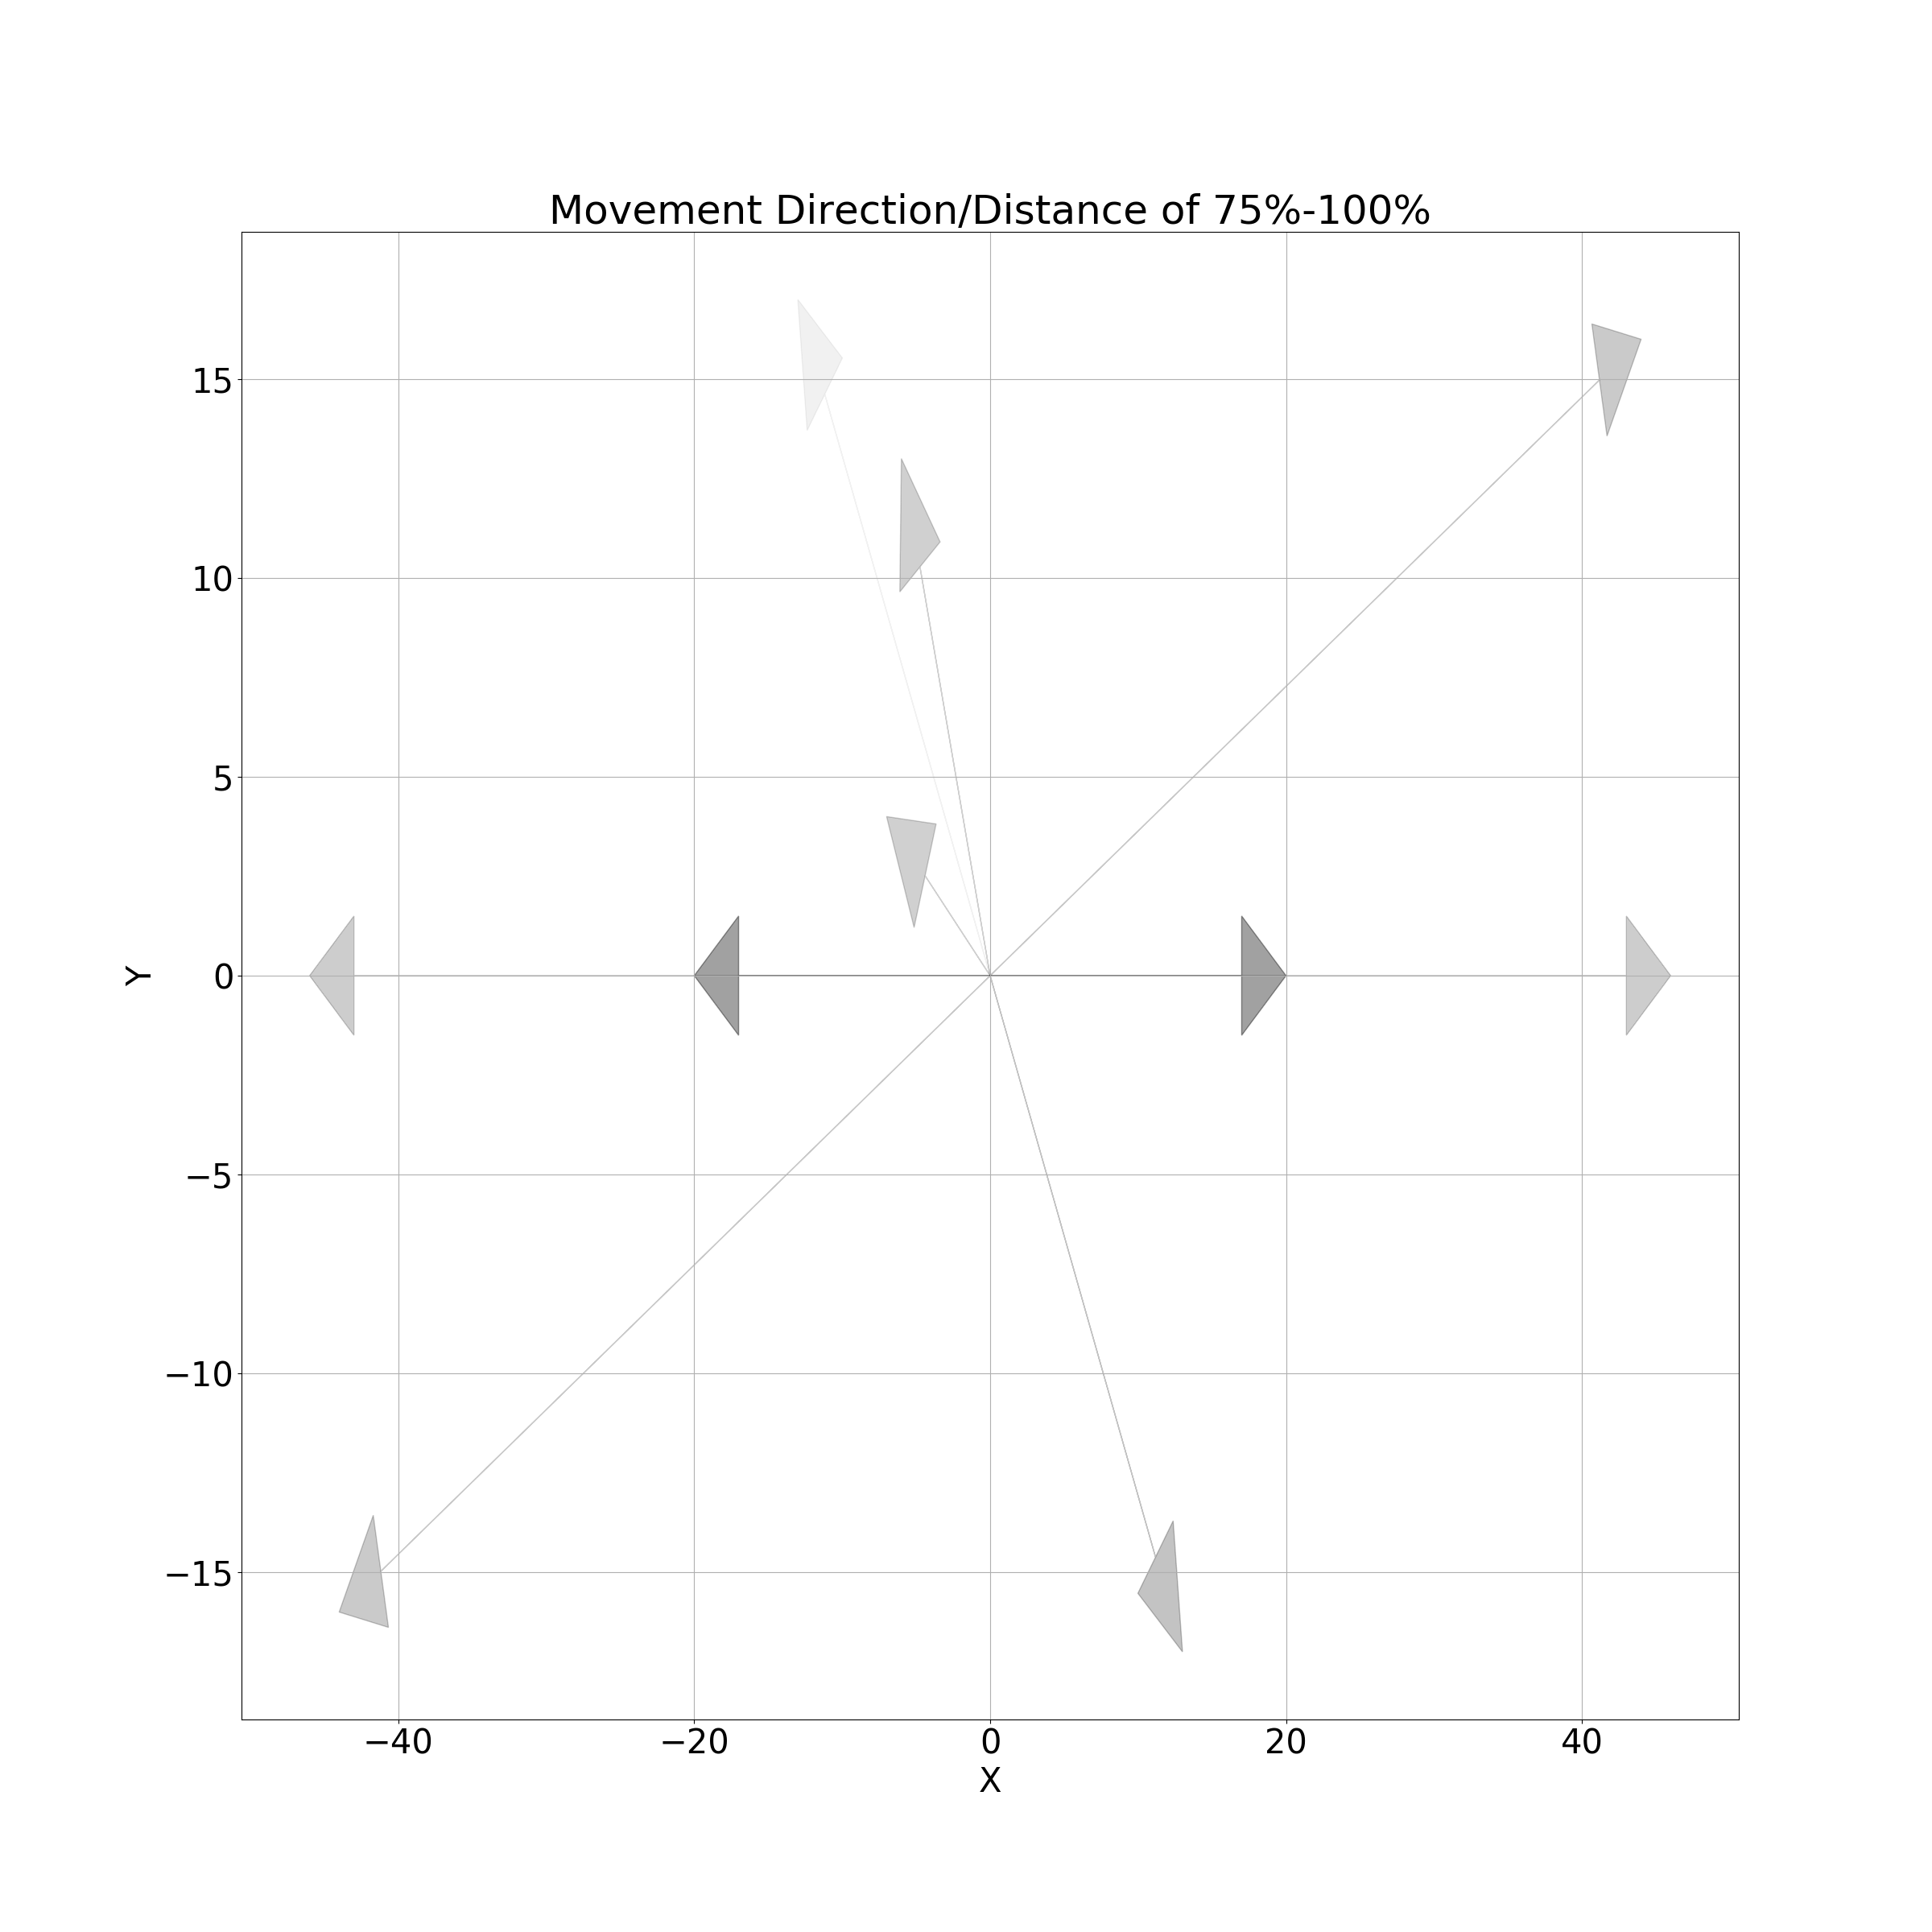
\includegraphics[width=0.3 \linewidth]{figures/movement3-4.png}
                    \\
                    
                    \mbox{(c) 50\%-75\%} & \mbox{(d) 75\%-100\%} \\
                \end{array}$
                \caption{Movement Direction/Distance on Third Floor}
                \label{fig:movedd3}
                \end{figure}
            
            \subsubsection{Department Distribution}
                There are seven departments in the data as followings: (in alphabetical)
                \begin{enumerate}
                    \item Administration
                    \item Engineering
                    \item Executive
                    \item Facilities
                    \item HR
                    \item Information Technology
                    \item Security
                \end{enumerate}
            
                Table \ref{tb:movequantile} shows the distribution of department by quartiles. Also, with the data in table \ref{tb:movequantile}, we drew the four pie plots as \ref{fig:department}.
                
                \begin{table}[htbp]
                    \centering
                    \caption{Department Information by Quartiles}
                    \label{tb:movequantile}
                    \begin{tabular}{c|cc}
                        Quartiles & Department & Counts \\ \hline
                        \multirow{4}{*}{q1 (Minimum 25\%)} & Administration & 8 \\
                        & Executive & 7 \\
                        & Facilities & 6 \\
                        & HR & 3 \\ \hline
                        \multirow{5}{*}{q2} & Engineering & 11 \\
                        & Security & 8 \\
                        & Administration & 6 \\
                        & Information Technology & 2 \\
                        & Facilities & 1 \\ \hline
                        \multirow{4}{*}{q3} & Information Technology & 12 \\
                        & Engineering & 7 \\
                        & Facilities & 5 \\
                        & Security & 2 \\ \hline
                        \multirow{4}{*}{q4 (Maximum 25\%)} & Engineering & 15 \\
                        & Facilities & 9 \\
                        & Information Technology & 3 \\
                        & Security & 1 \\
                    \end{tabular}
                \end{table}
                
                \begin{figure}[htbp]
                    \centering
                    $\begin{array}{cccc}
                        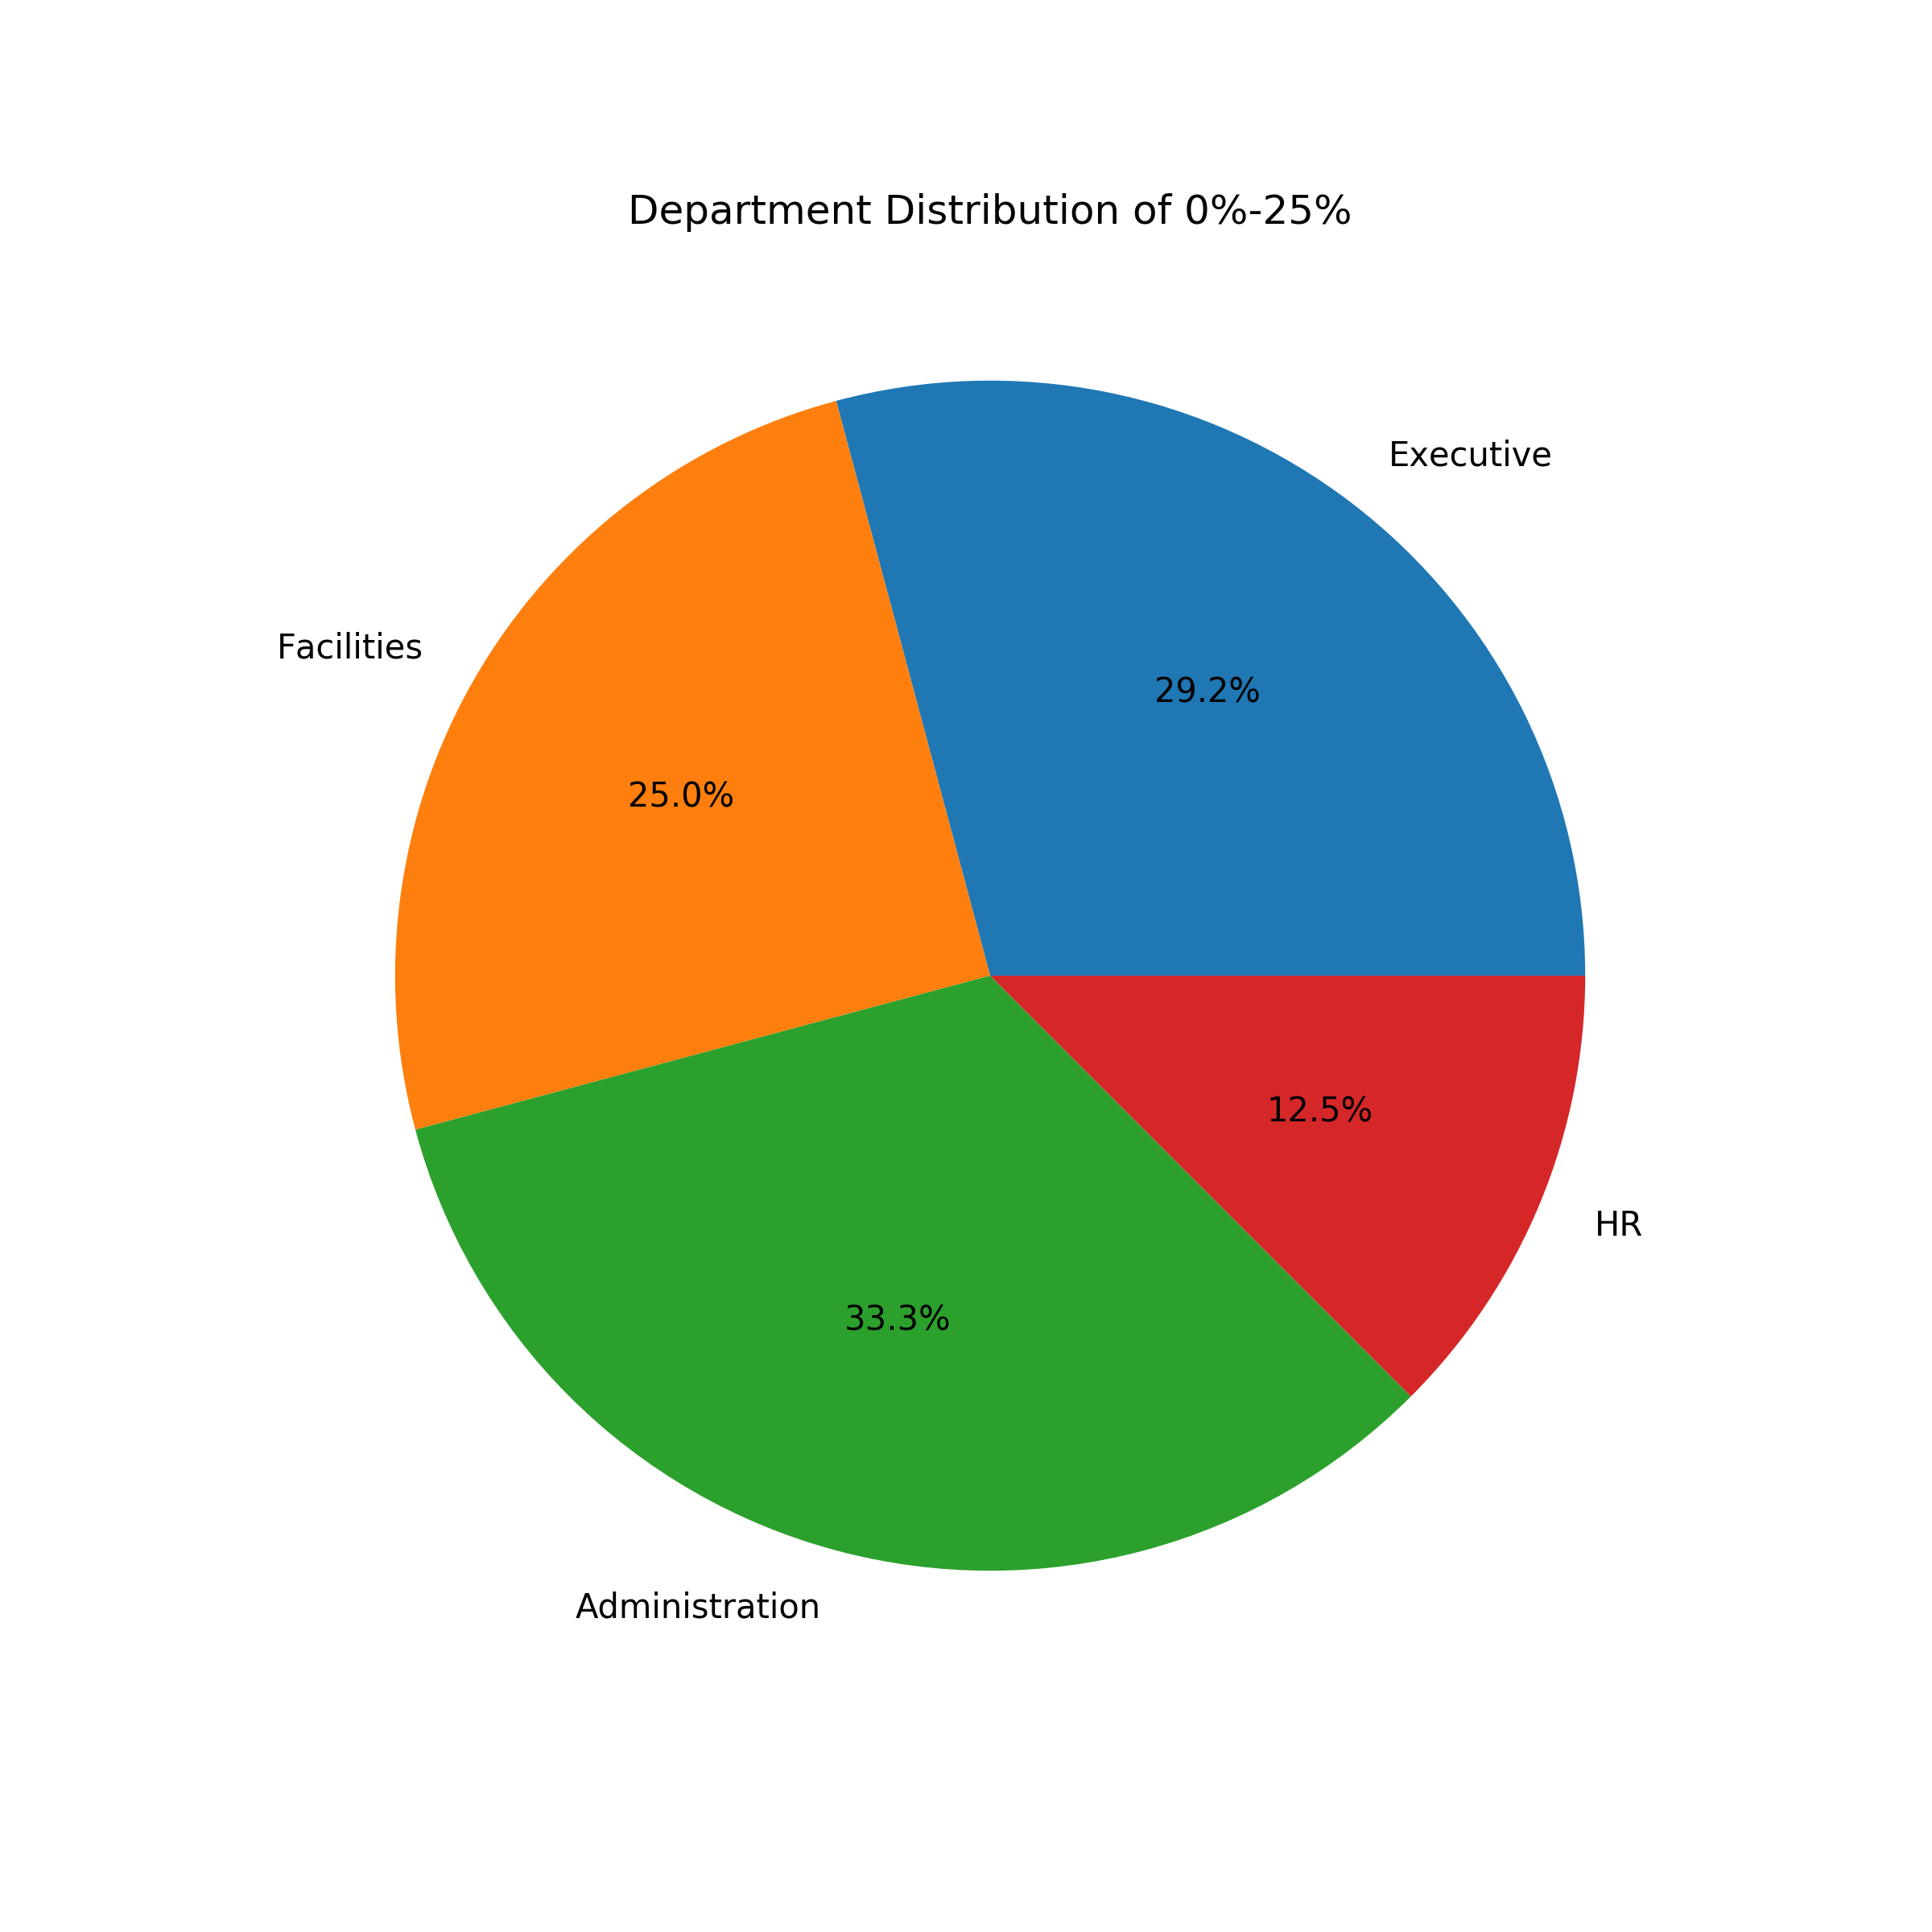
\includegraphics[width=0.2 \linewidth]{figures/department1.png}
                        &
                        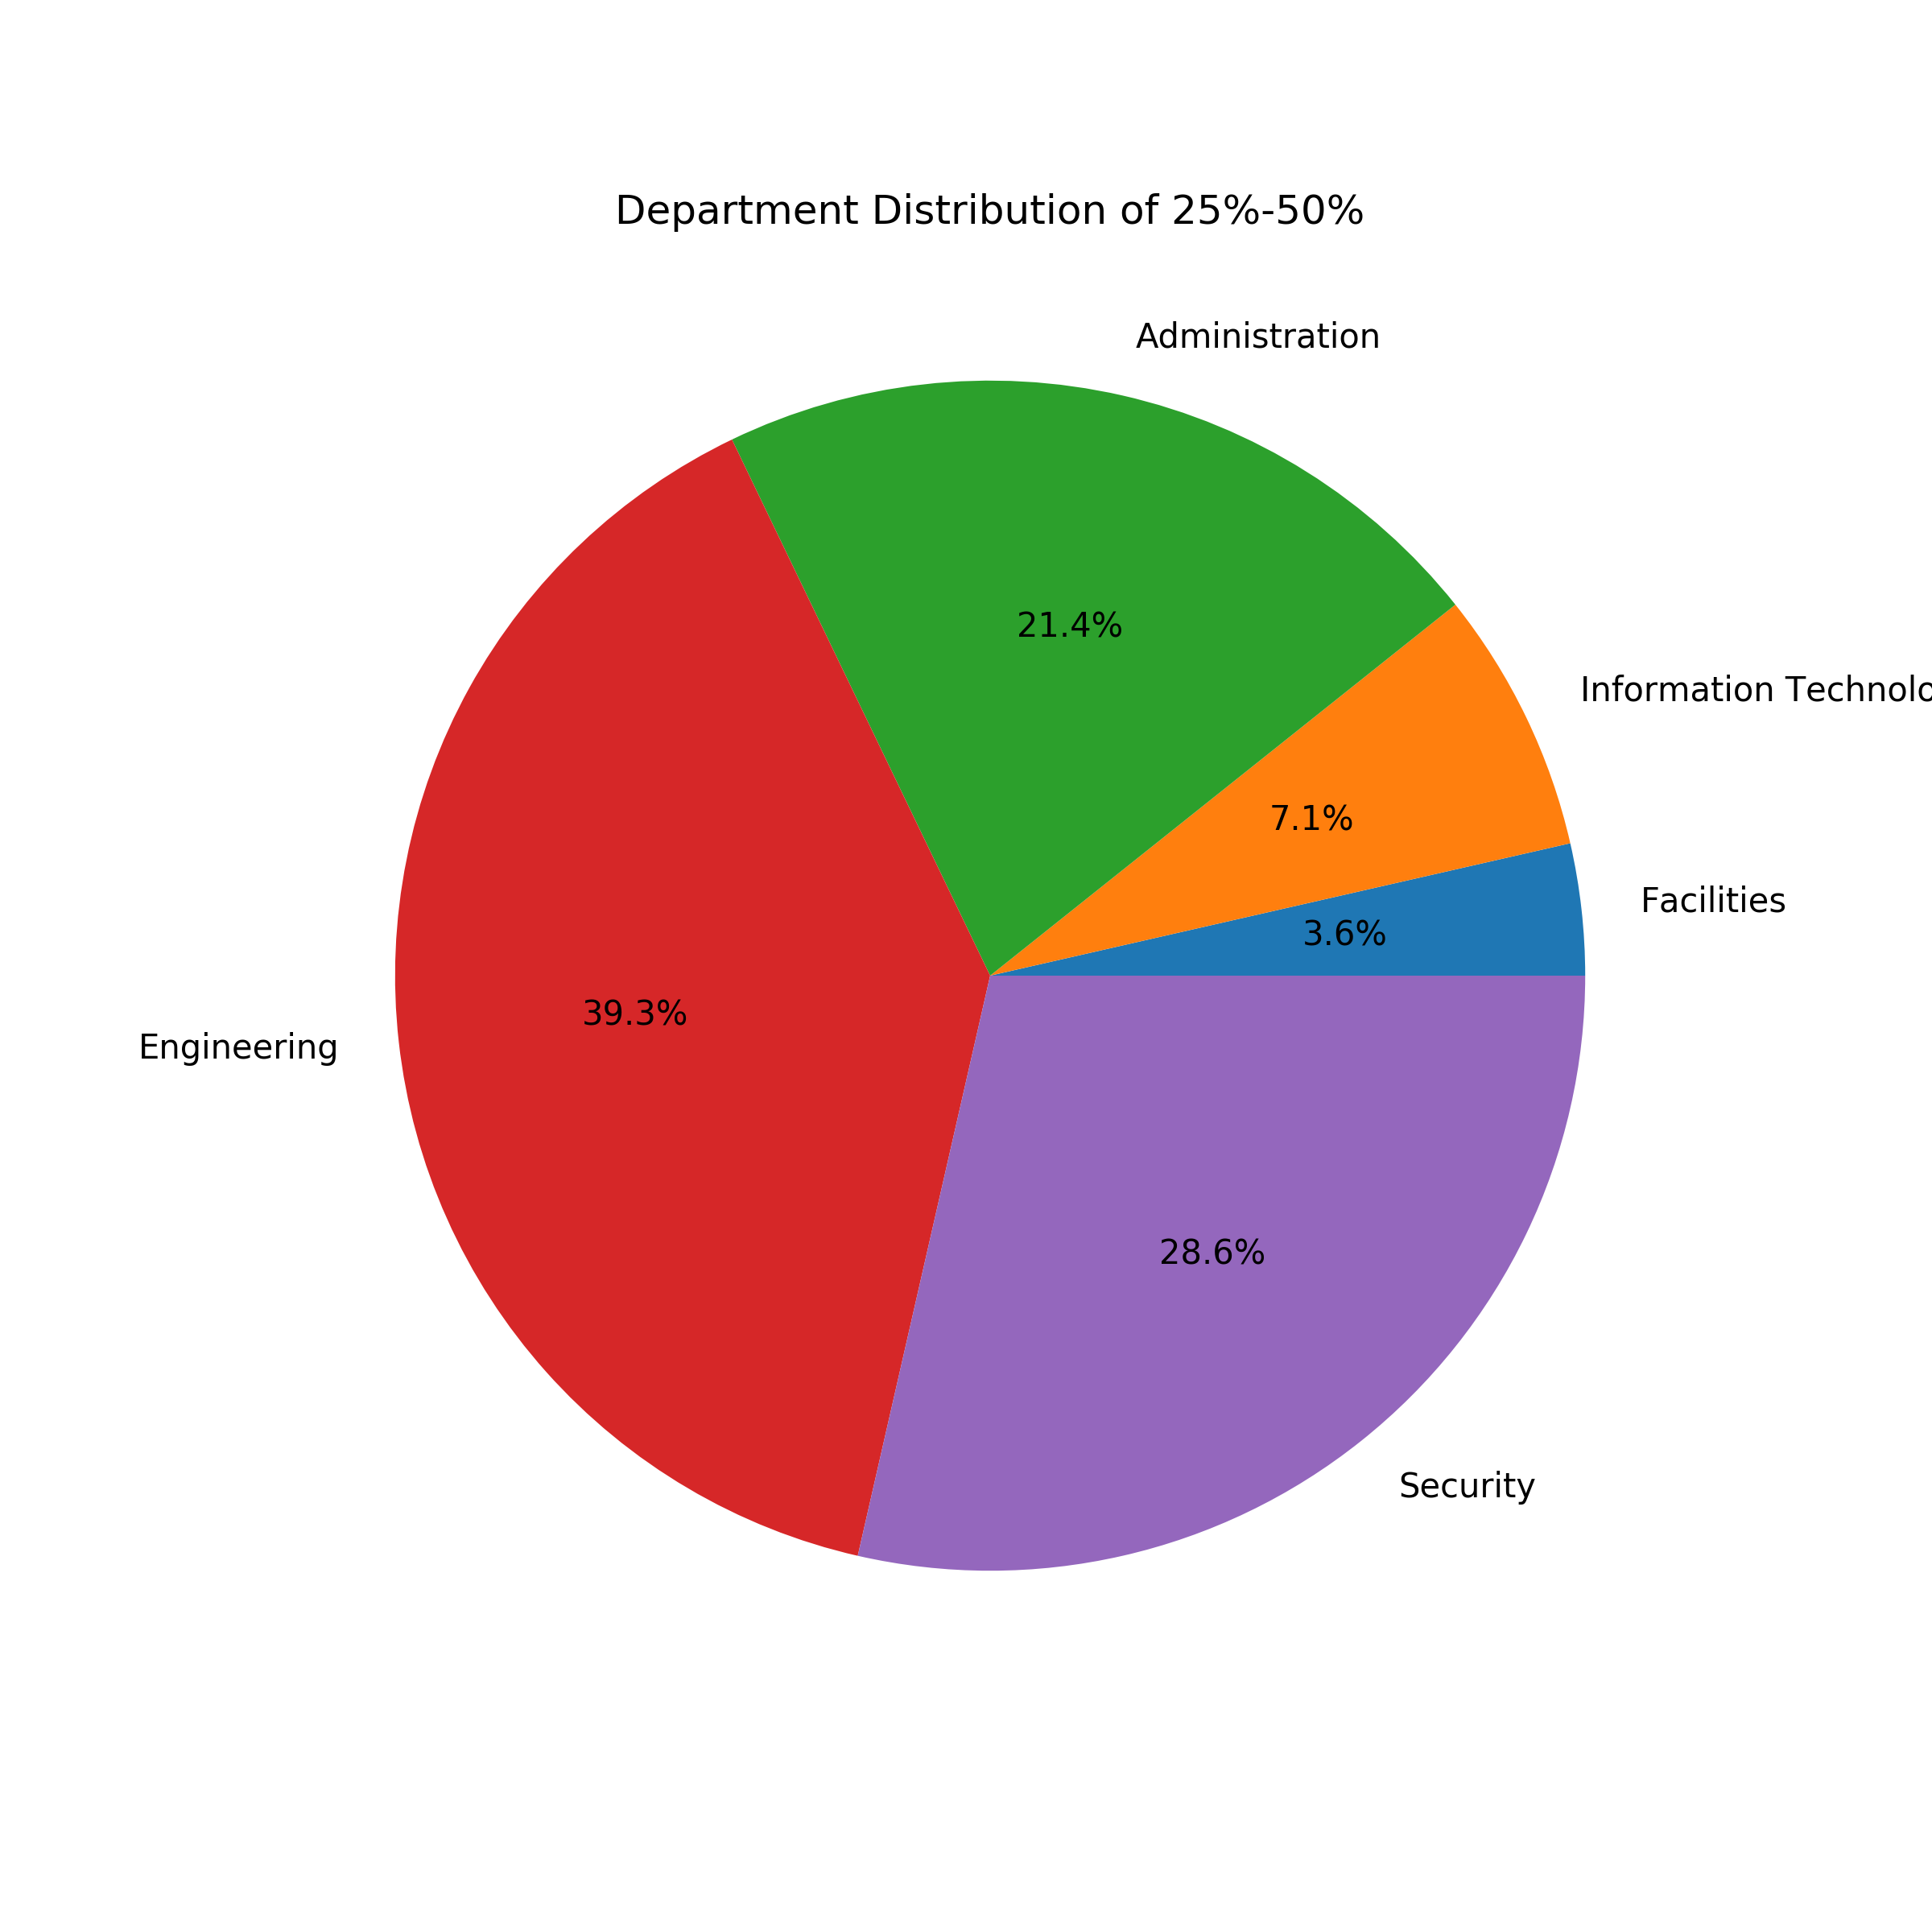
\includegraphics[width=0.2 \linewidth]{figures/department2.png}
                        &
                        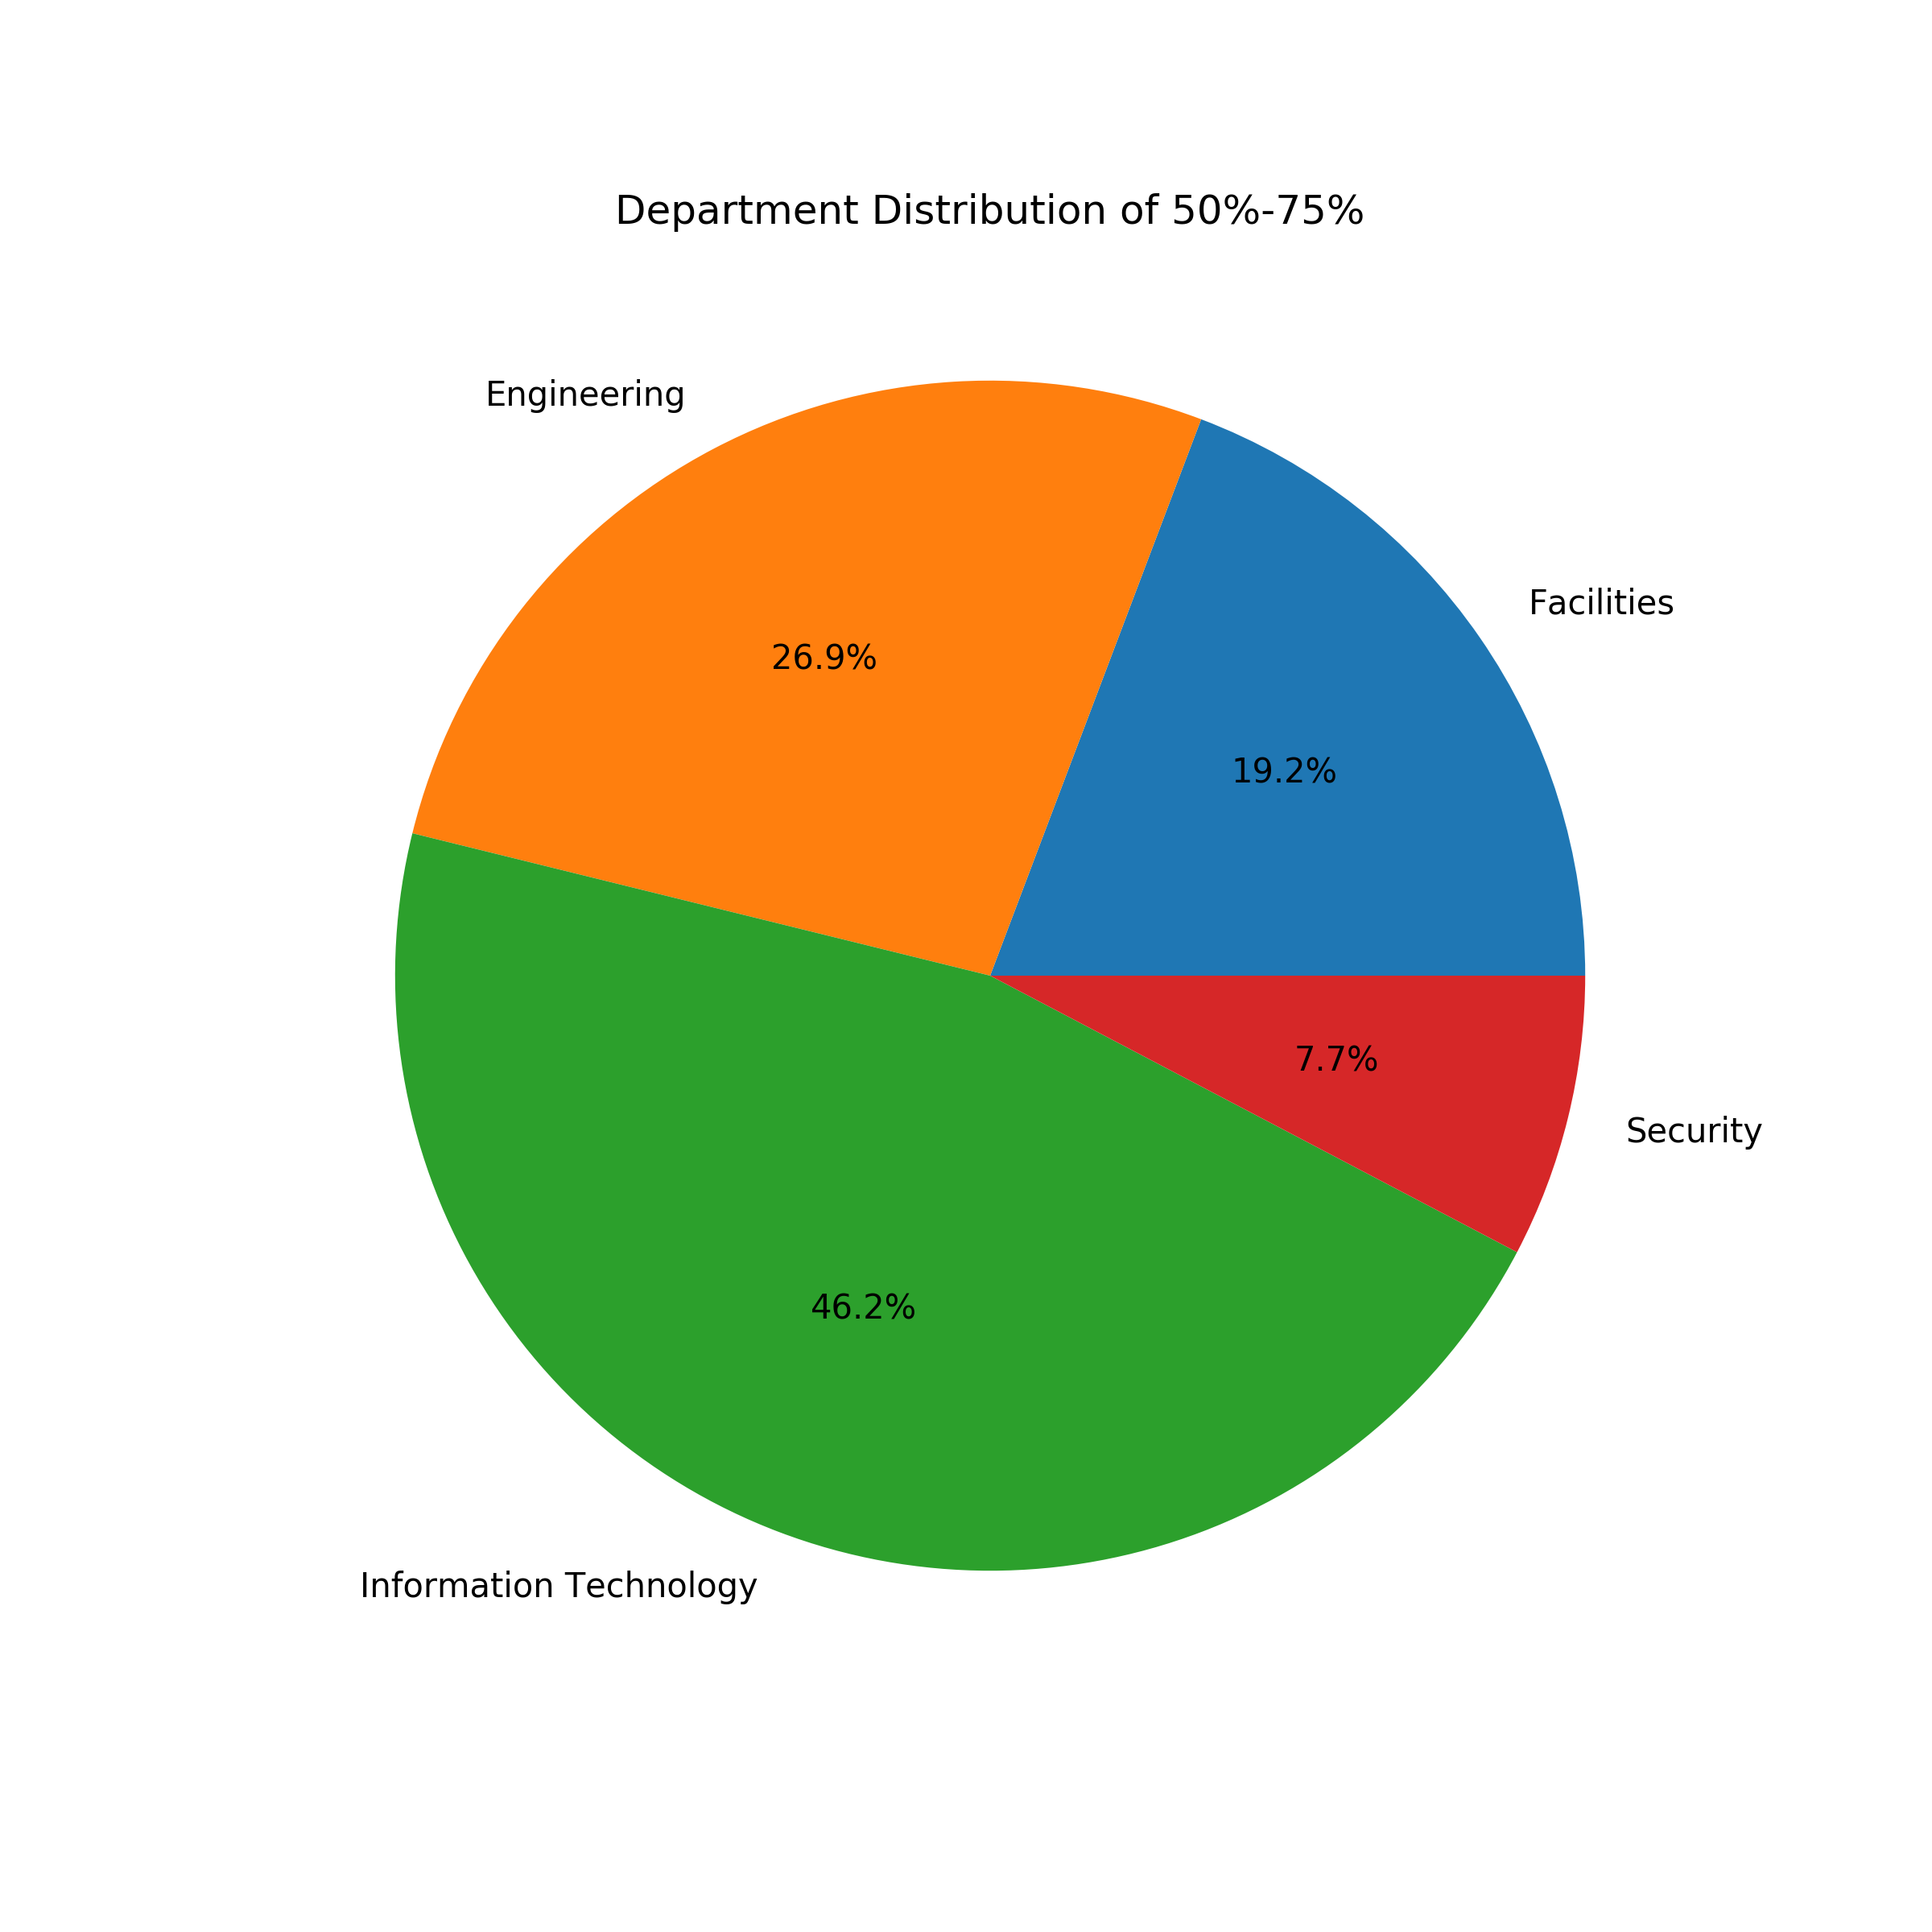
\includegraphics[width=0.2 \linewidth]{figures/department3.png}
                        &
                        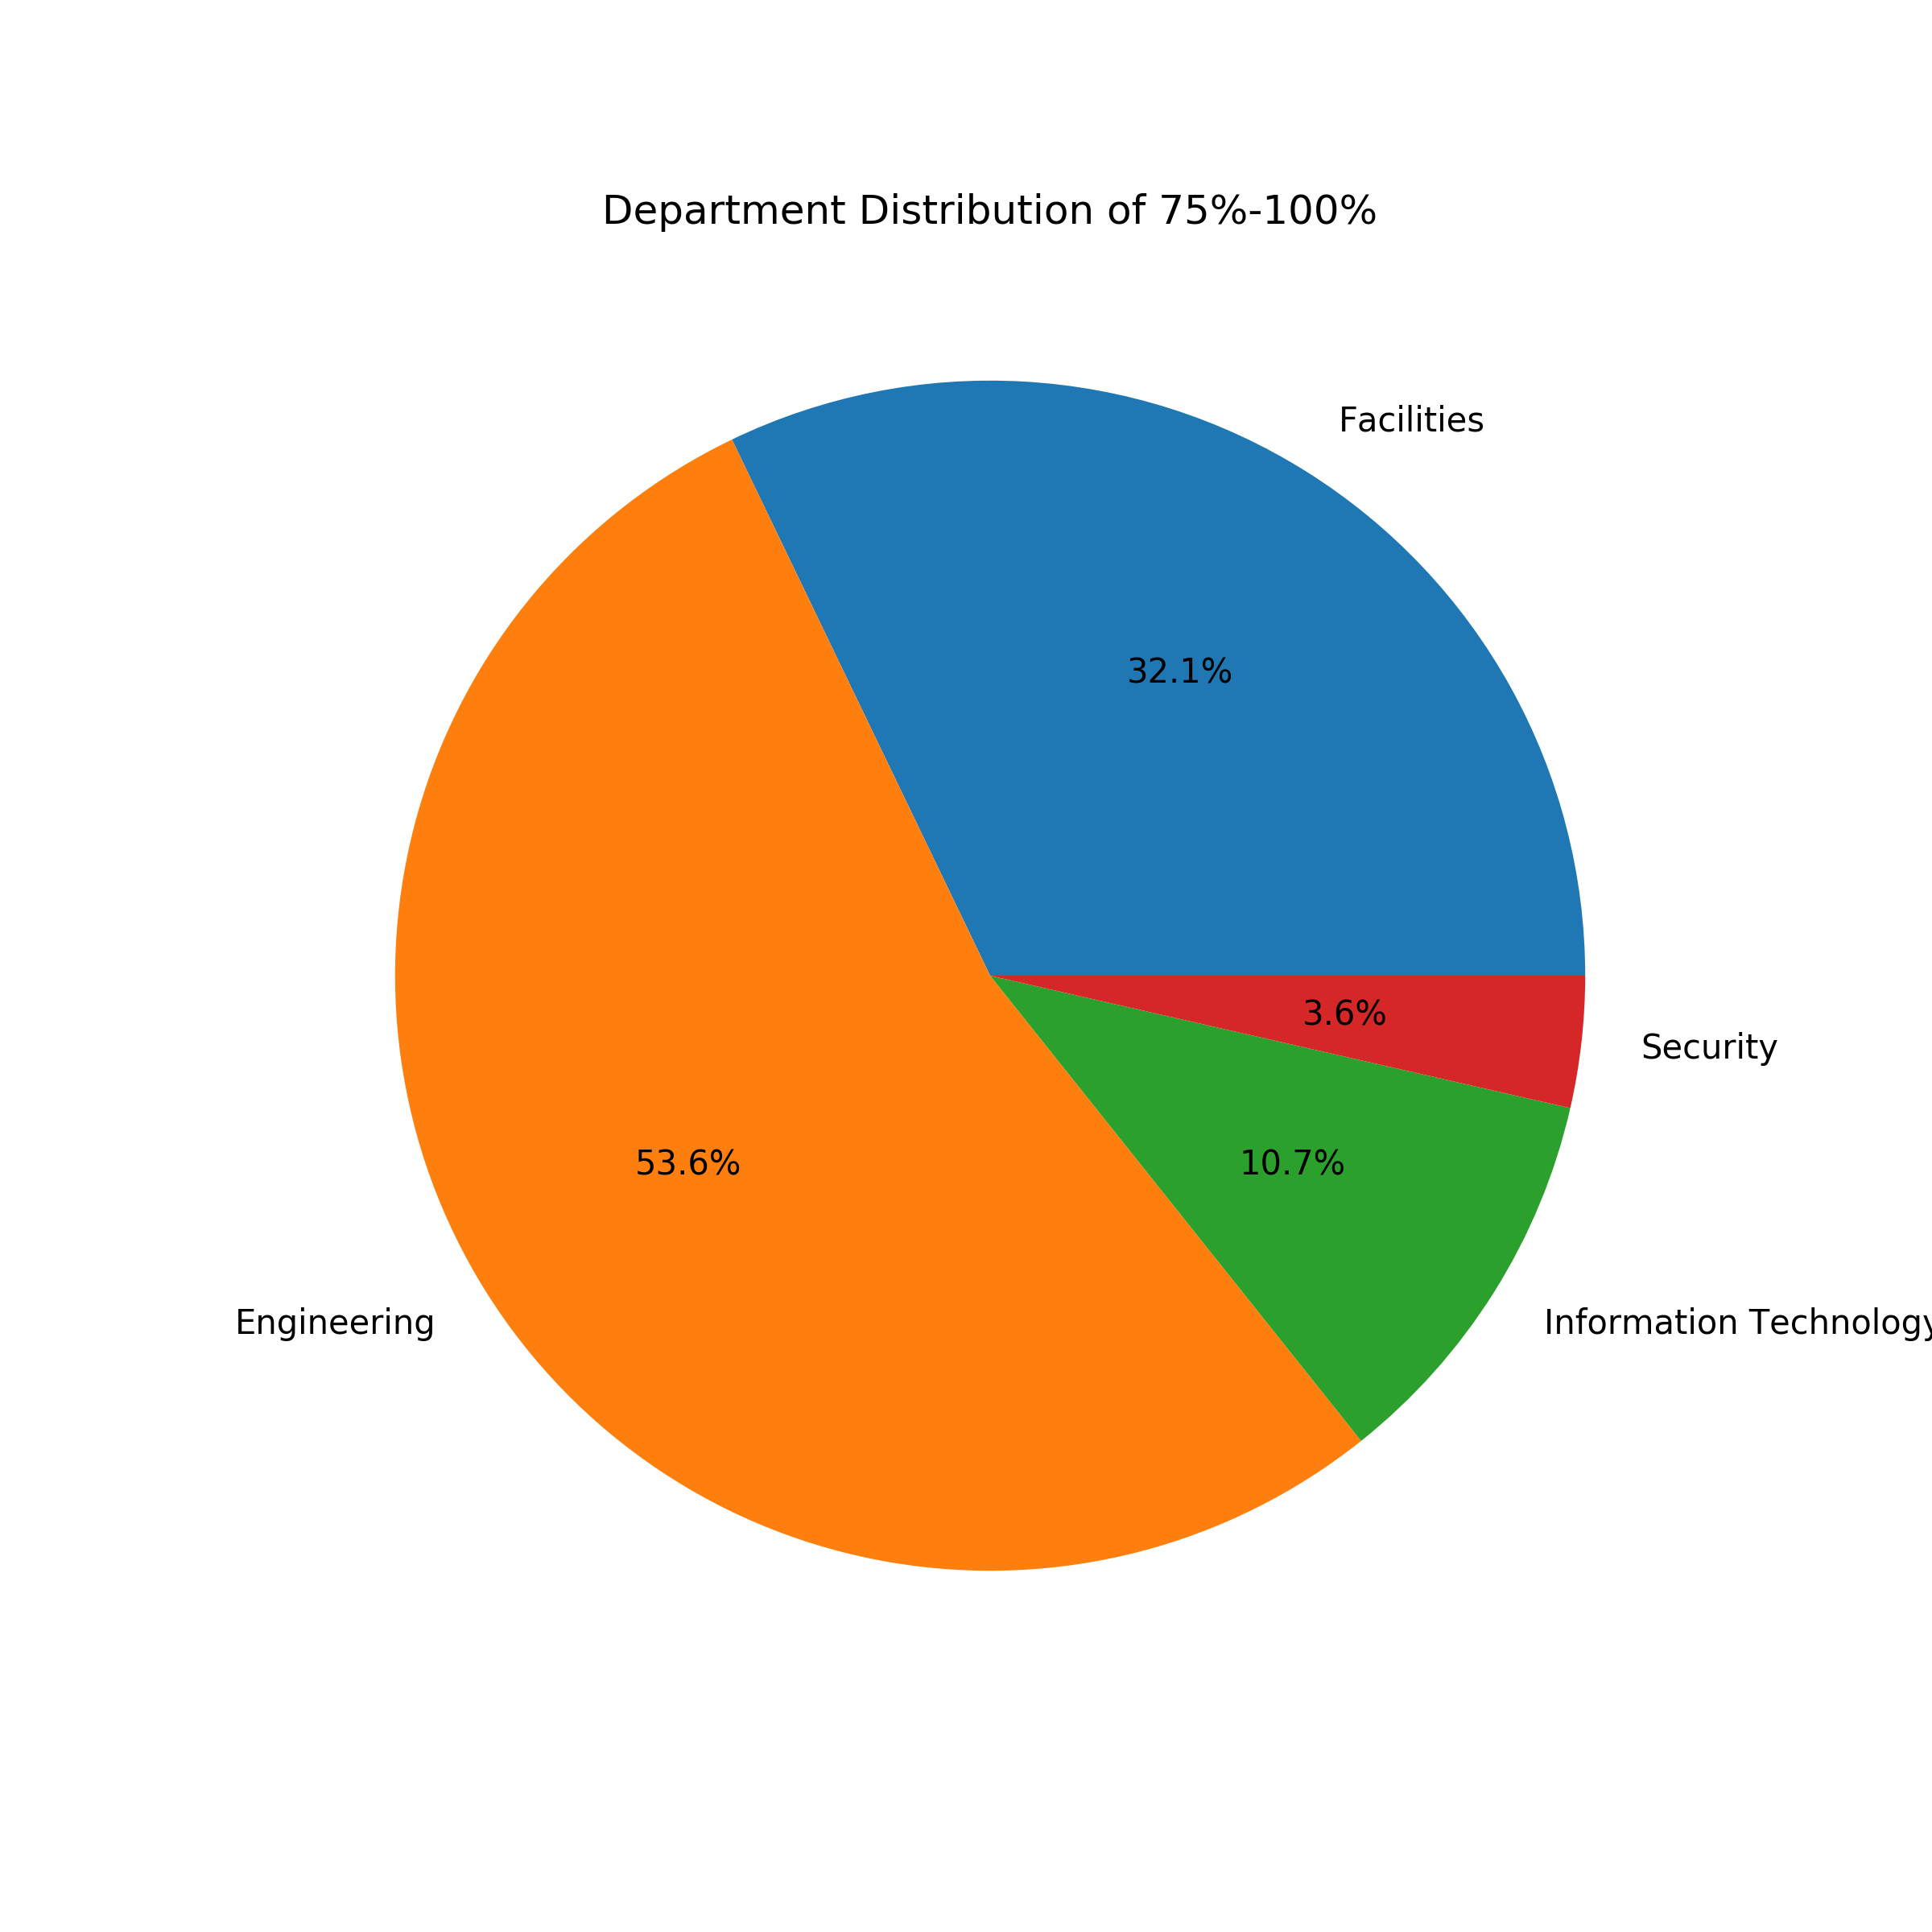
\includegraphics[width=0.2 \linewidth]{figures/department4.png}
                        \\
                        
                        \mbox{(a) q1} & \mbox{(b) q2} & \mbox{(c) q3} & \mbox{(d) q4} \\
                    \end{array}$
                    \caption{Pie Plot of Department Distribution by Quartiles}
                    \label{fig:department}
                \end{figure}
            
            \subsubsection{Typical Day Look for GAStech employees}
                First of all, when you look at prox card data by floor, there is a hub which almost everyone goes through. This pattern is most common on the second floor, with prox zone 1 going through the center the most. One can assume that this is because it is just in front of the elevator's entrance and is a passageway linking each office. Also, this is an area that must be passed if you use an elevator when you go to wok or go home. 
                
                \begin{figure}[htbp]
                    \centering
                    $\begin{array}{ccc}
                        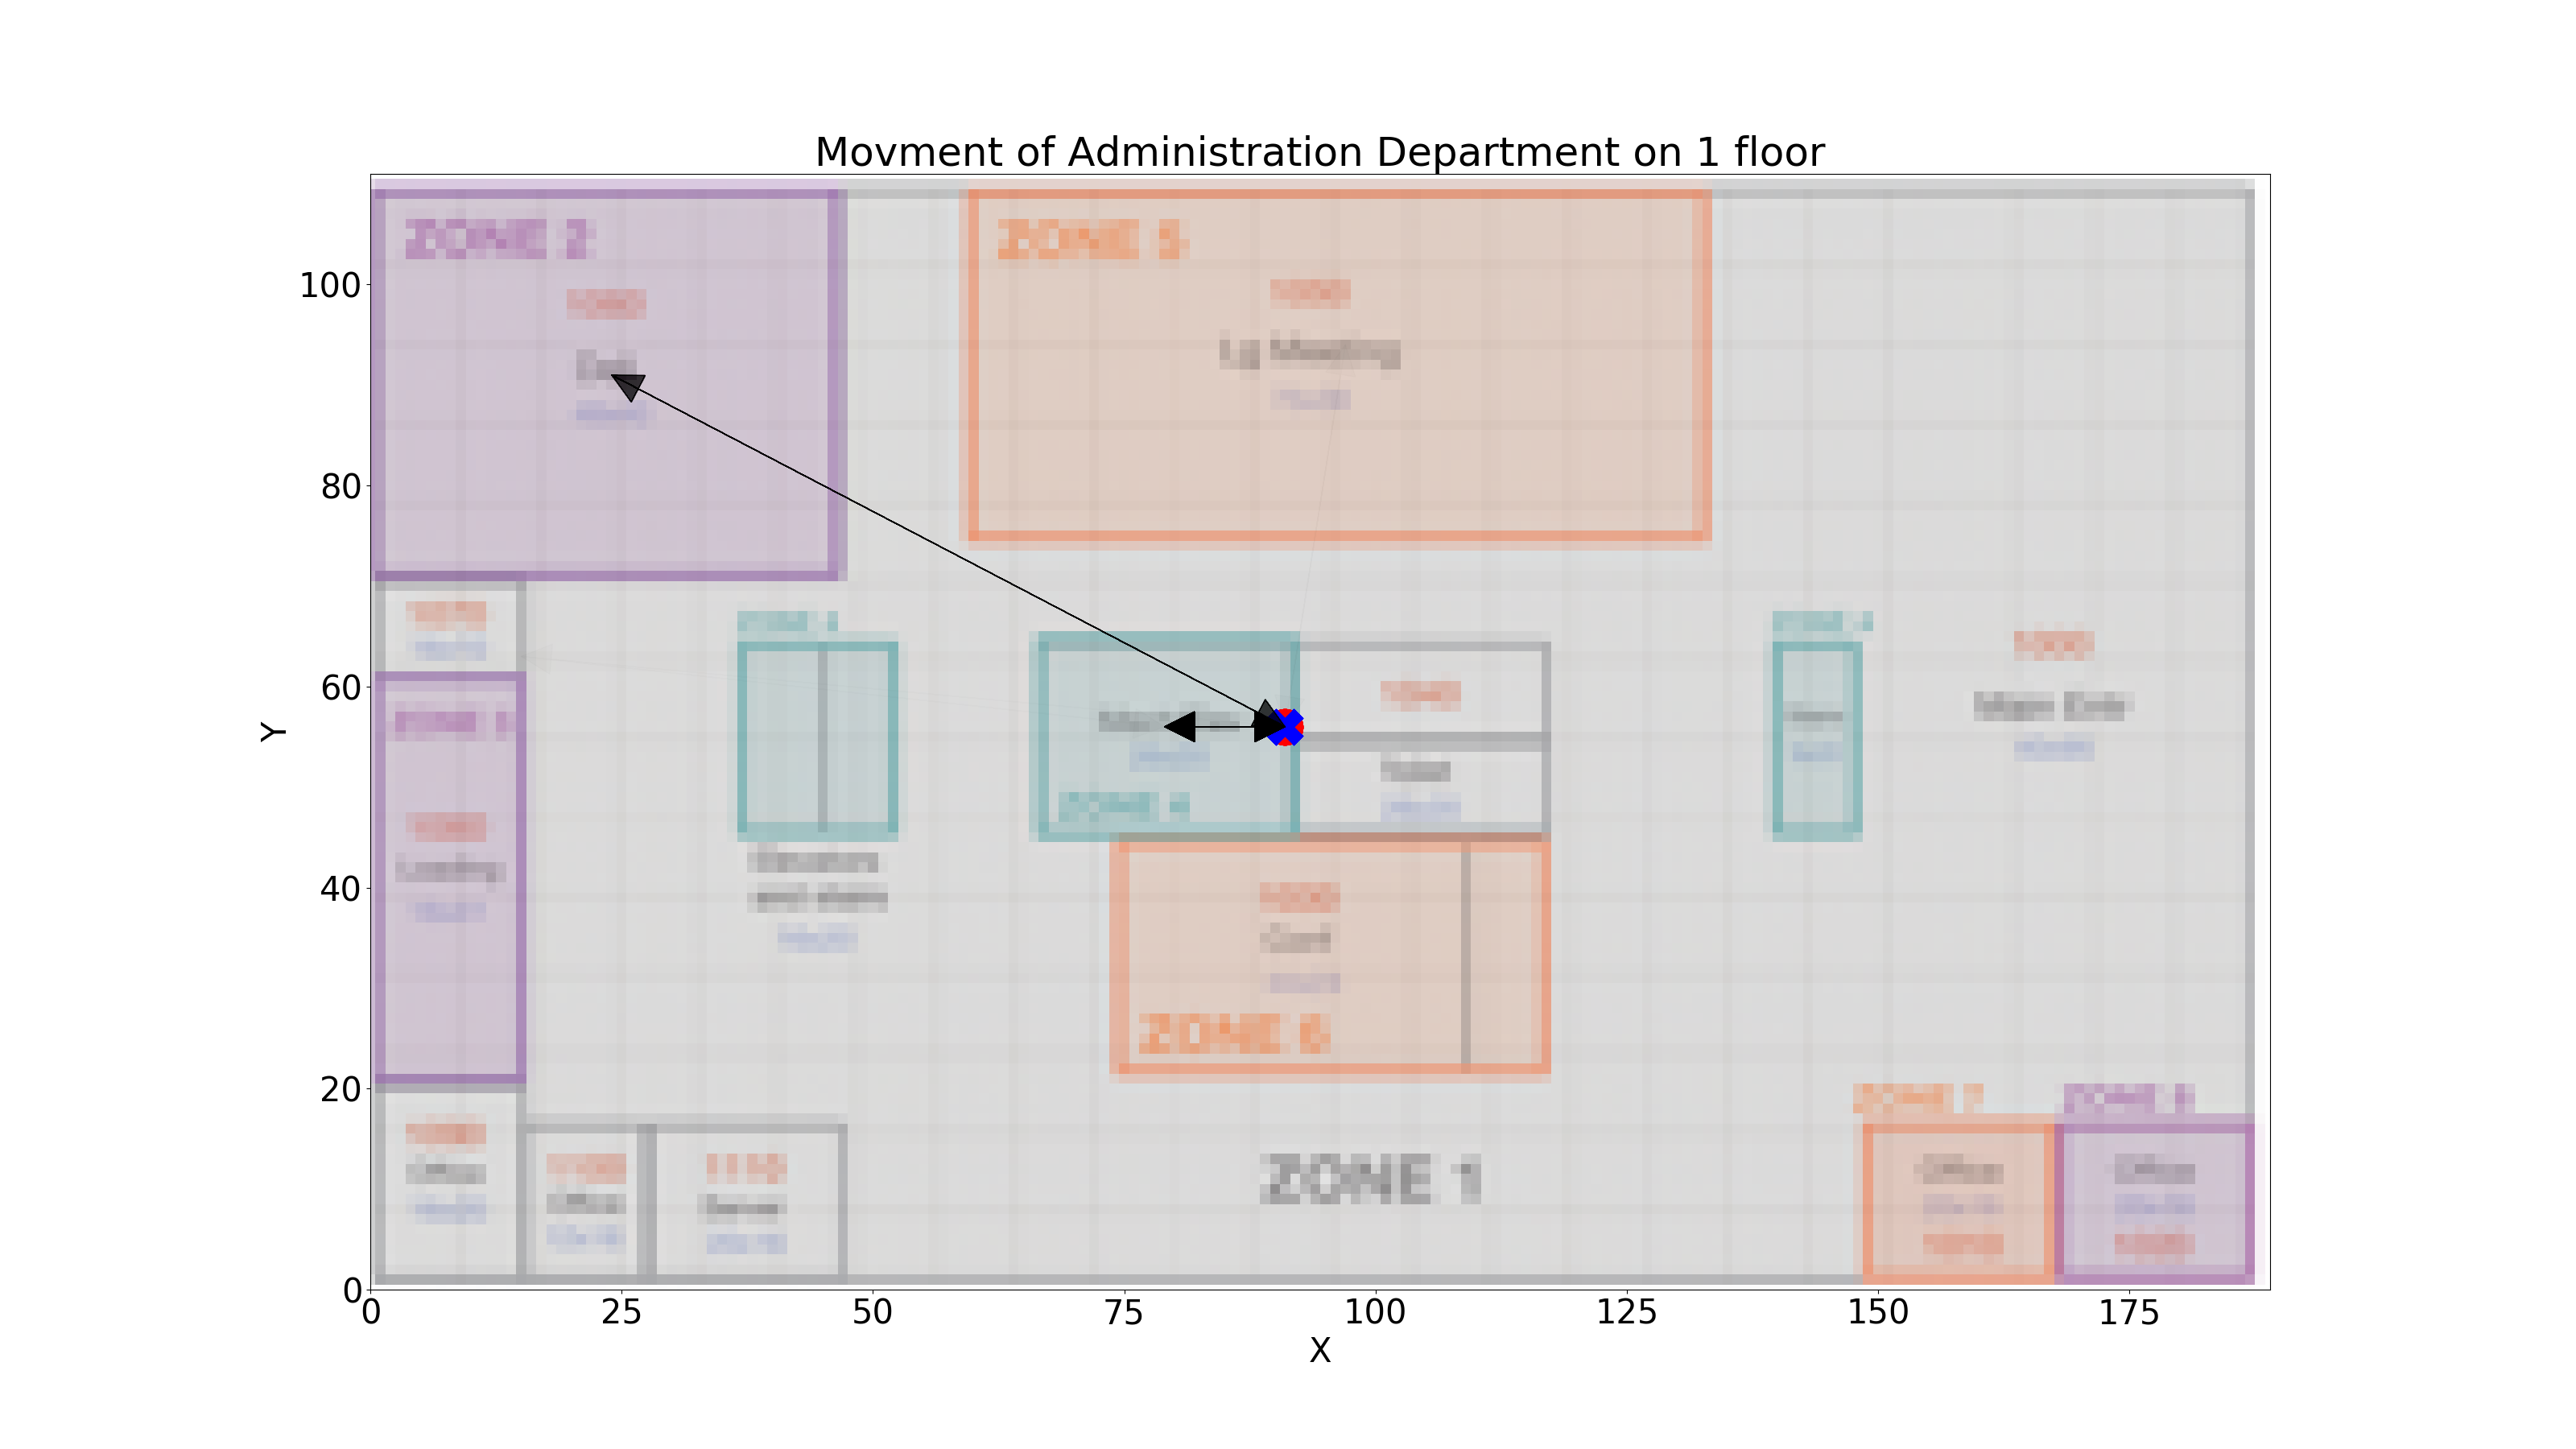
\includegraphics[width=0.3 \linewidth]{figures/Administration1.png}
                        &
                        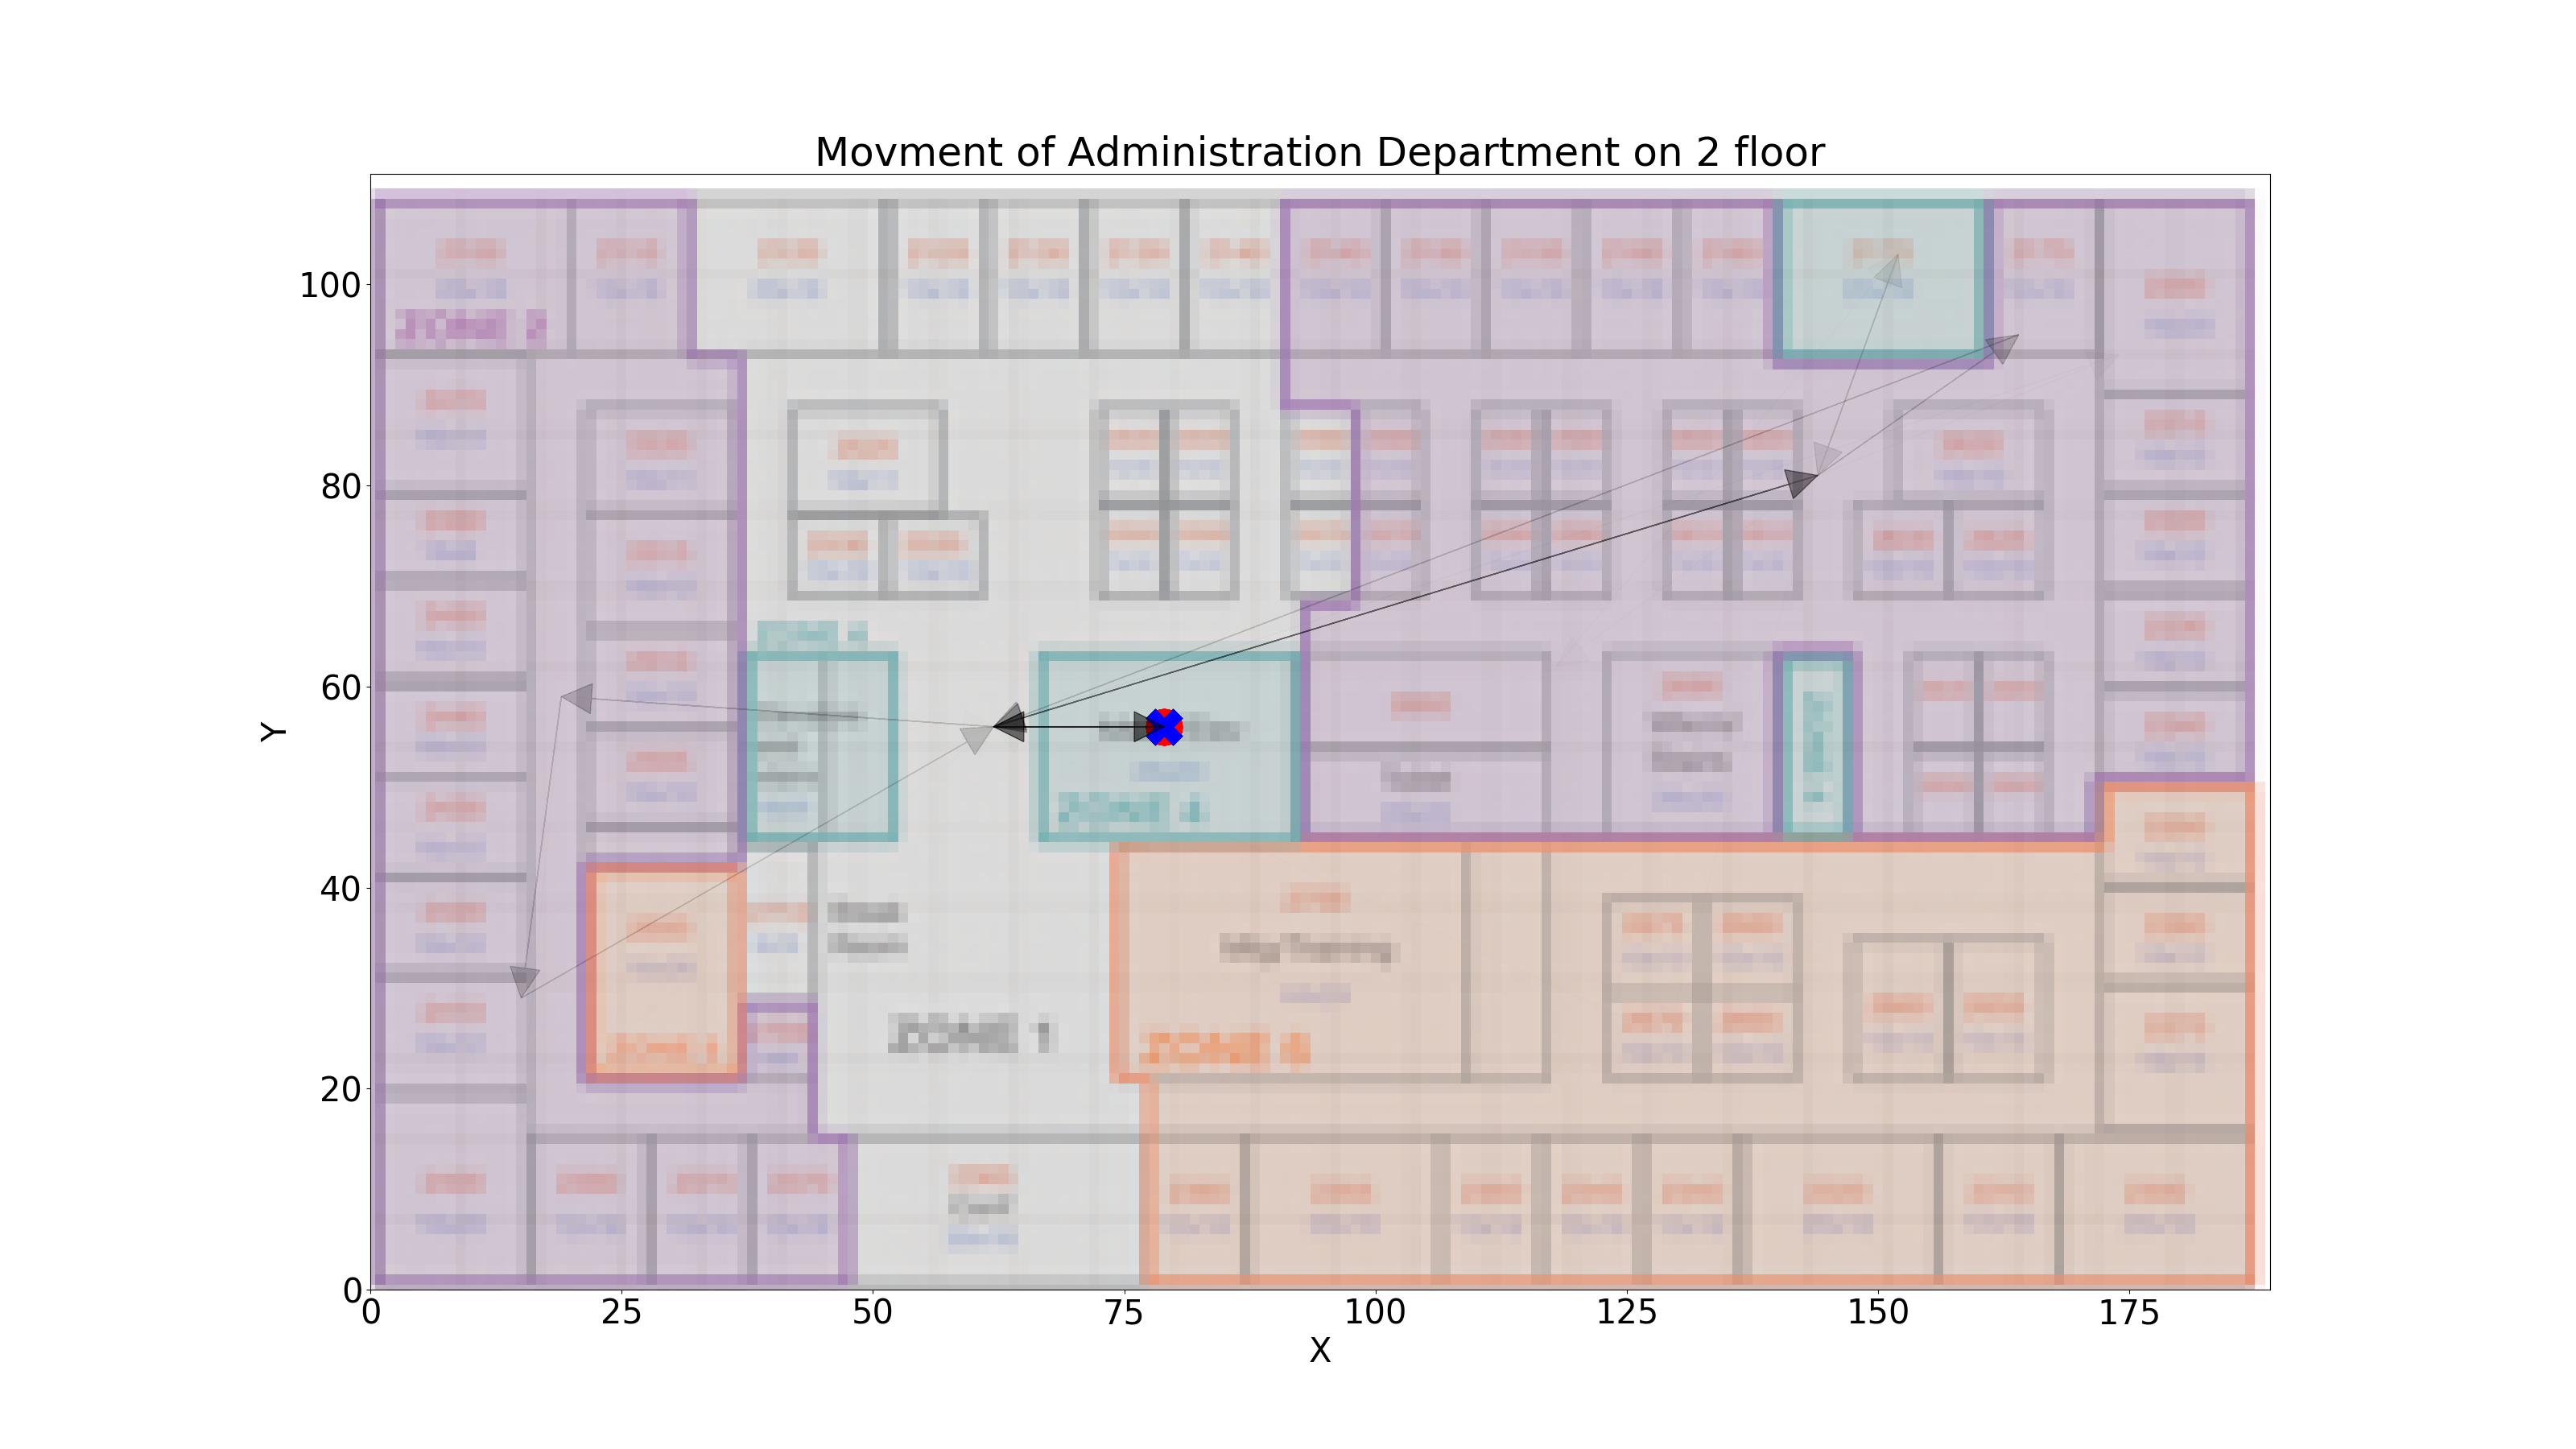
\includegraphics[width=0.3 \linewidth]{figures/Administration2.png}
                        &
                        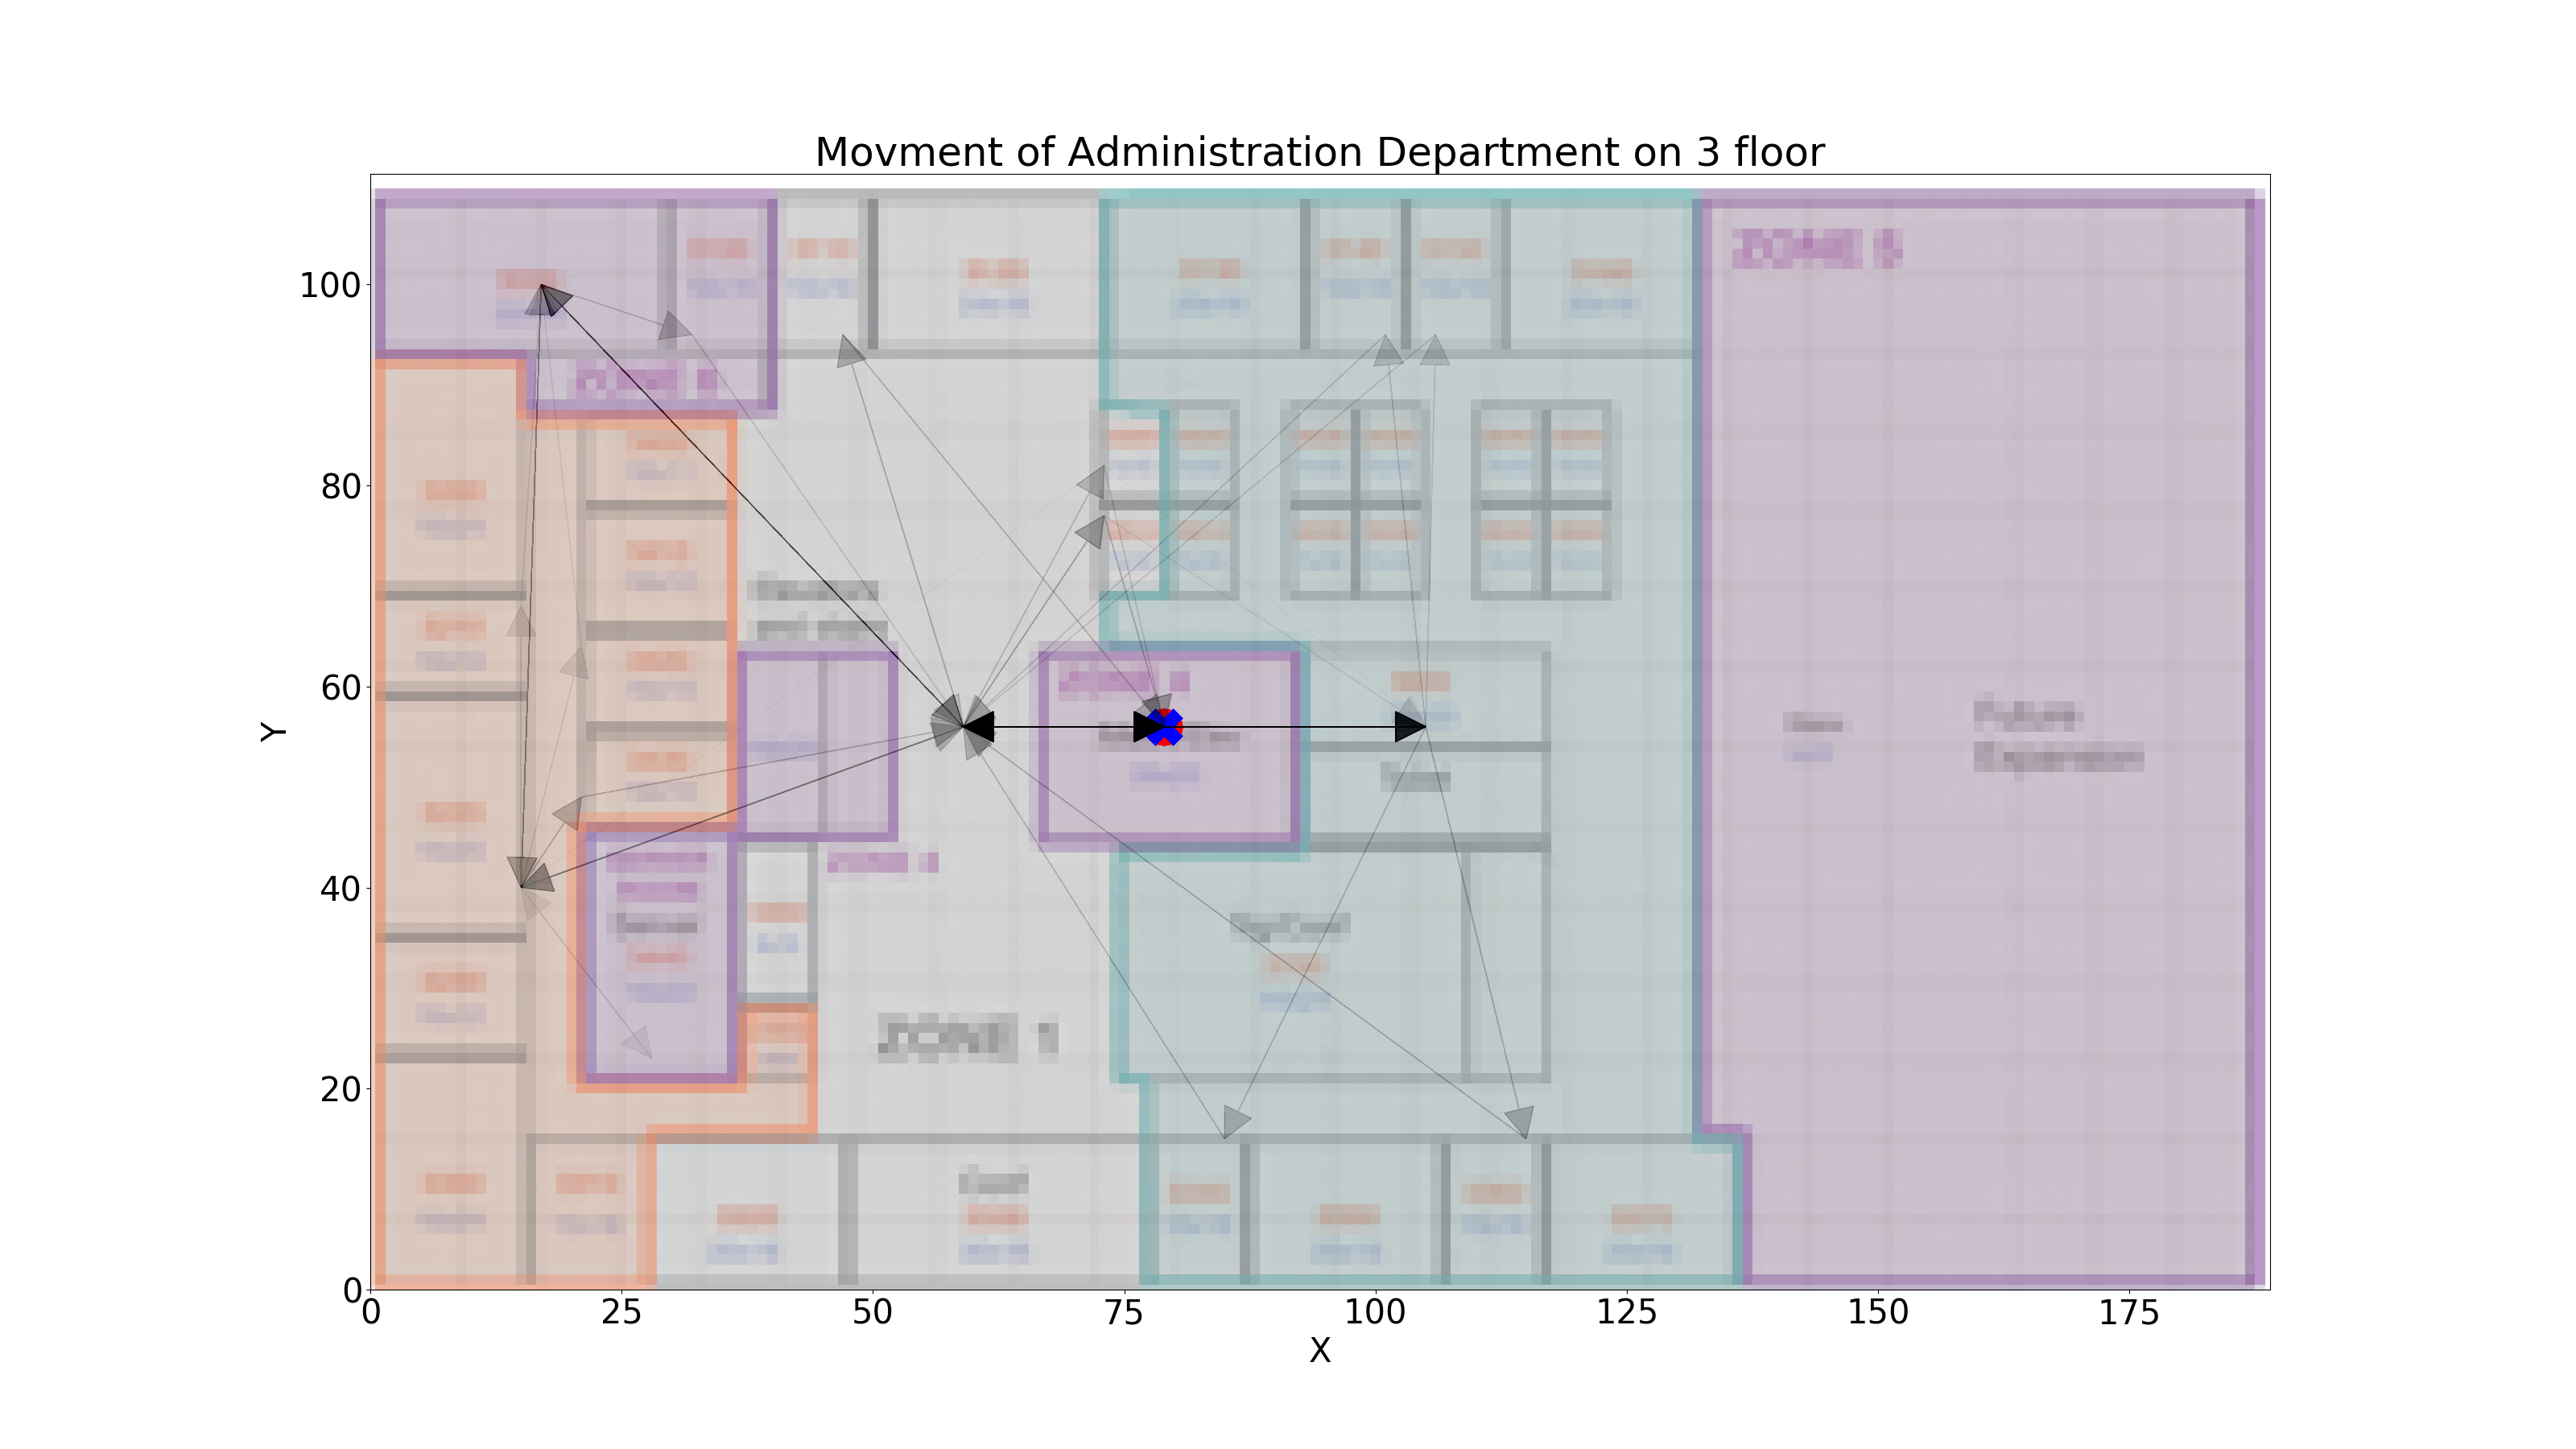
\includegraphics[width=0.3 \linewidth]{figures/Administration3.png}
                        \\
                        
                        \mbox{(a) First Floor} & \mbox{(b) Second Floor} & \mbox{(c) Third Floor} \\
                    \end{array}$
                    \caption{Movement within Administration Department}
                    \label{fig:admin}
                \end{figure}
                
                \begin{figure}[htbp]
                    \centering
                    $\begin{array}{ccc}
                        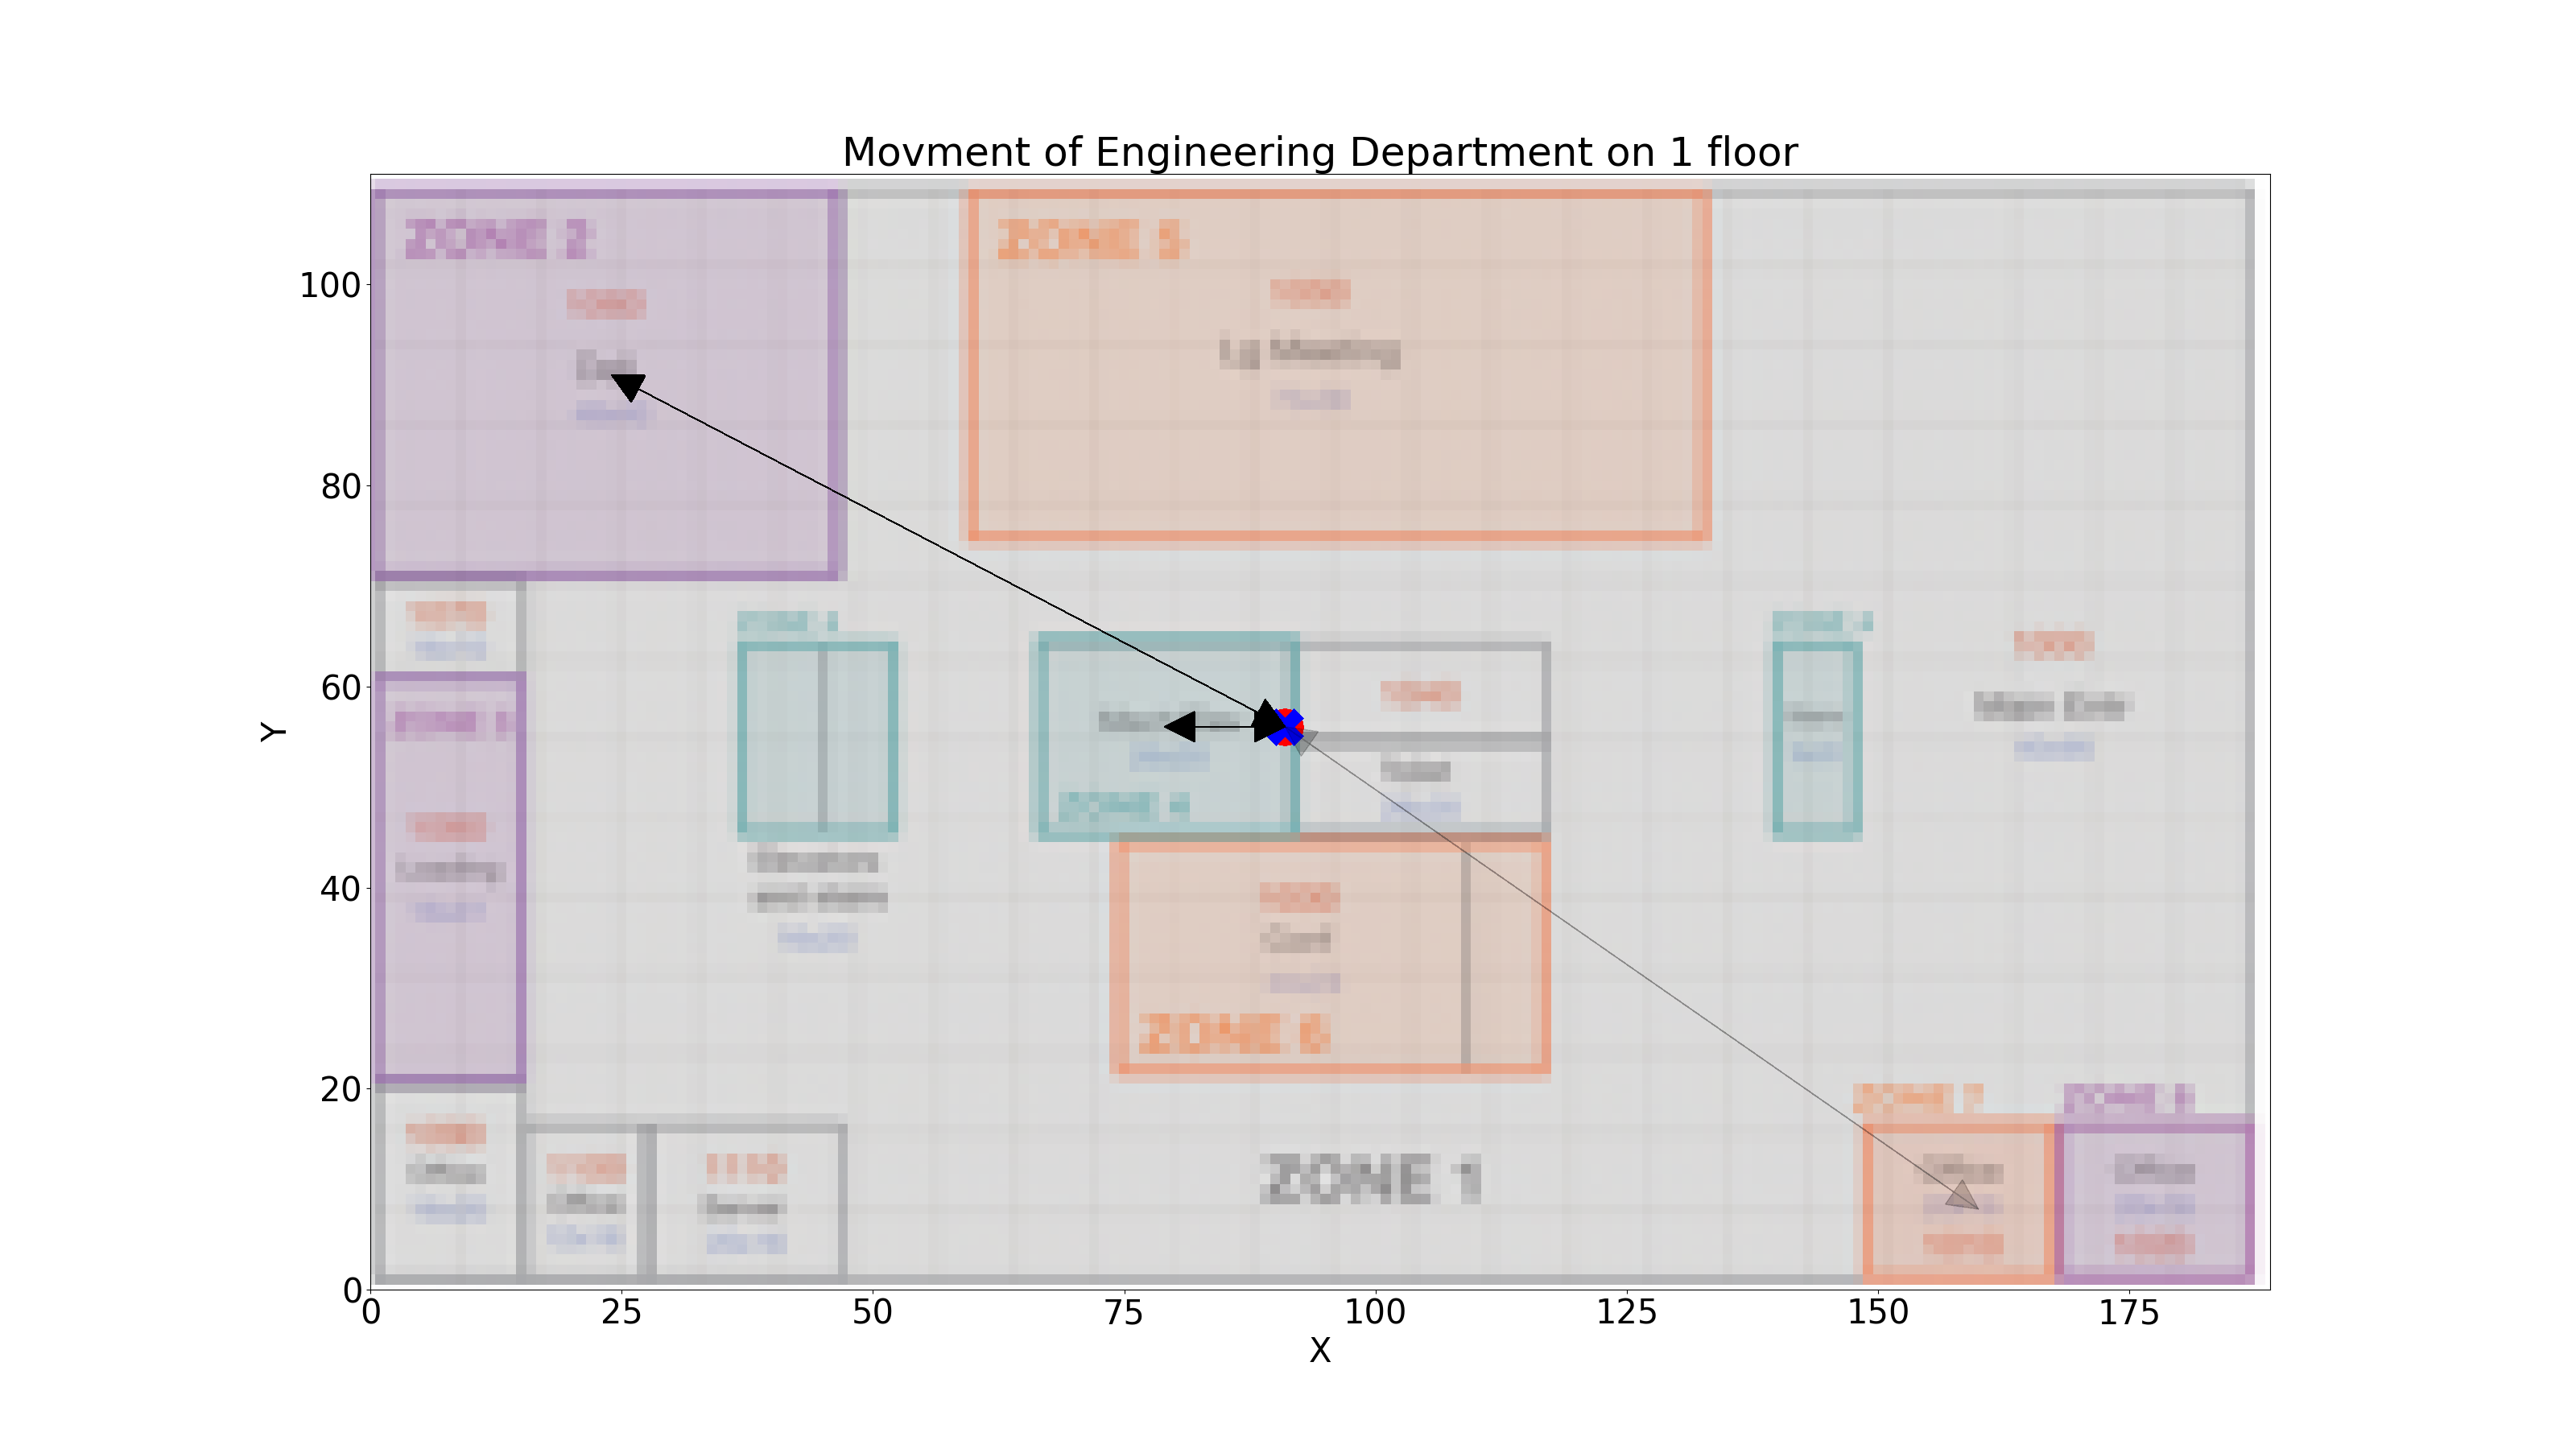
\includegraphics[width=0.3 \linewidth]{figures/Engineering1.png}
                        &
                        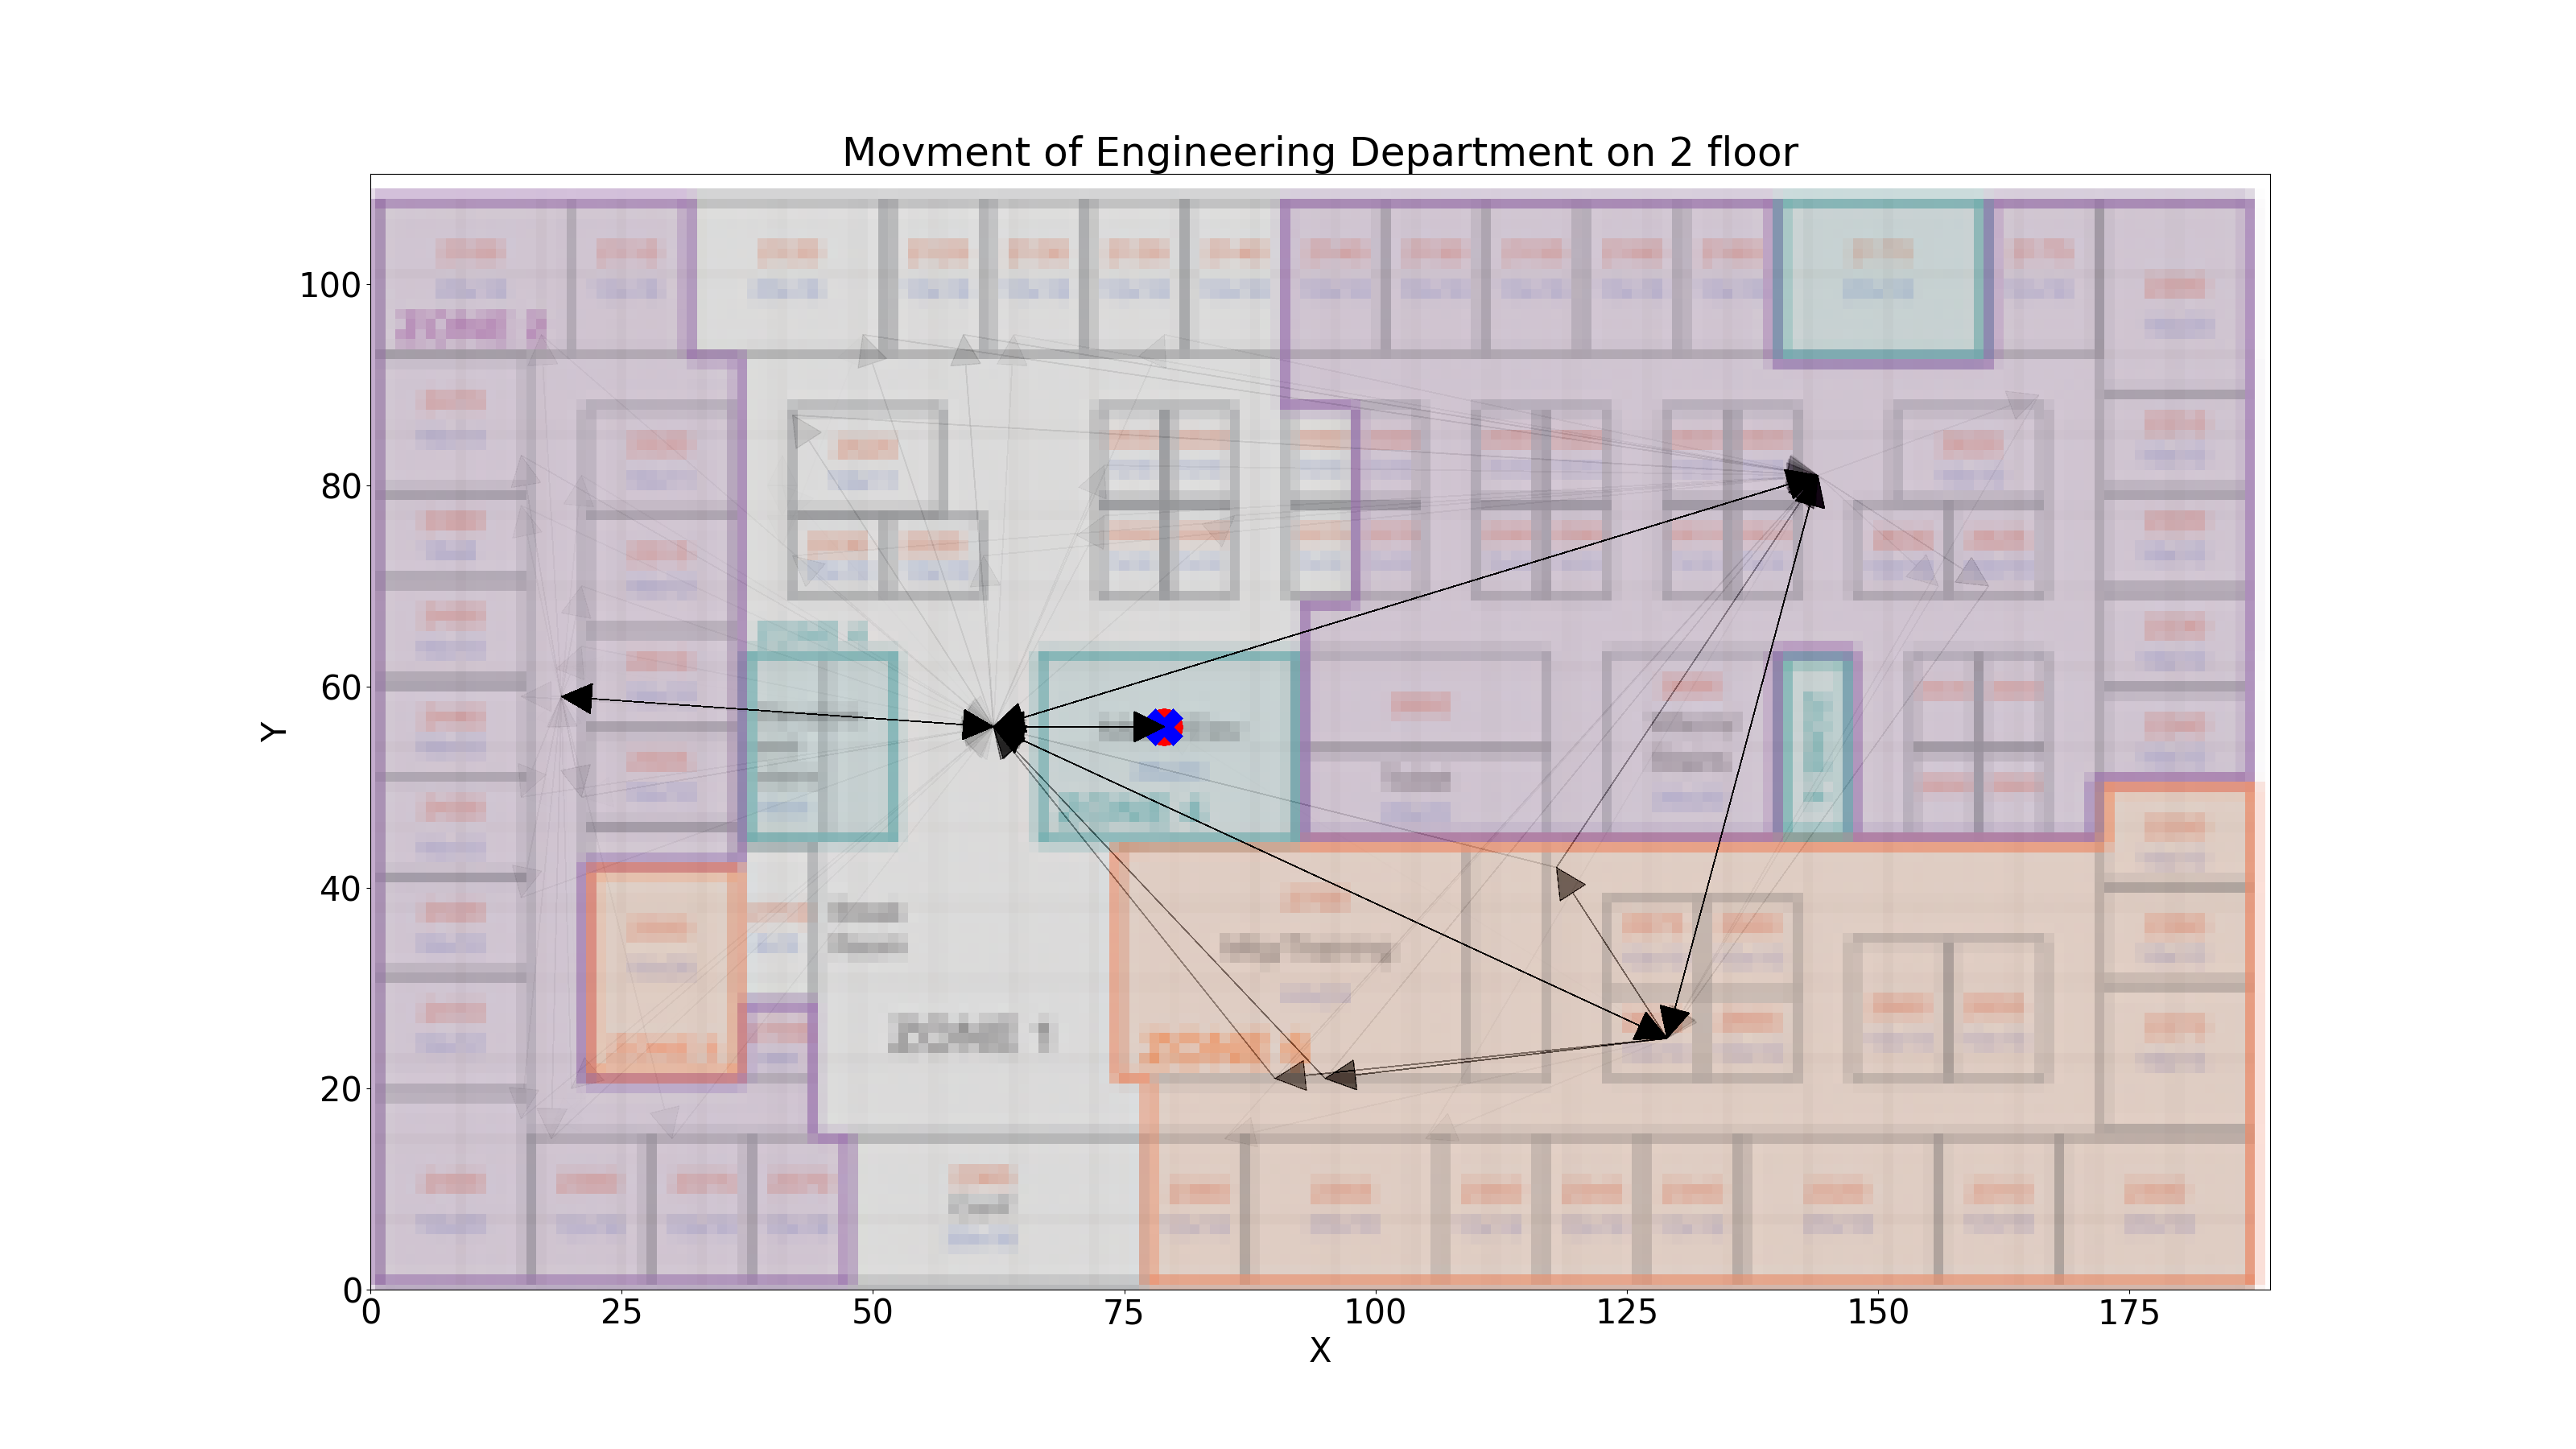
\includegraphics[width=0.3 \linewidth]{figures/Engineering2.png}
                        &
                        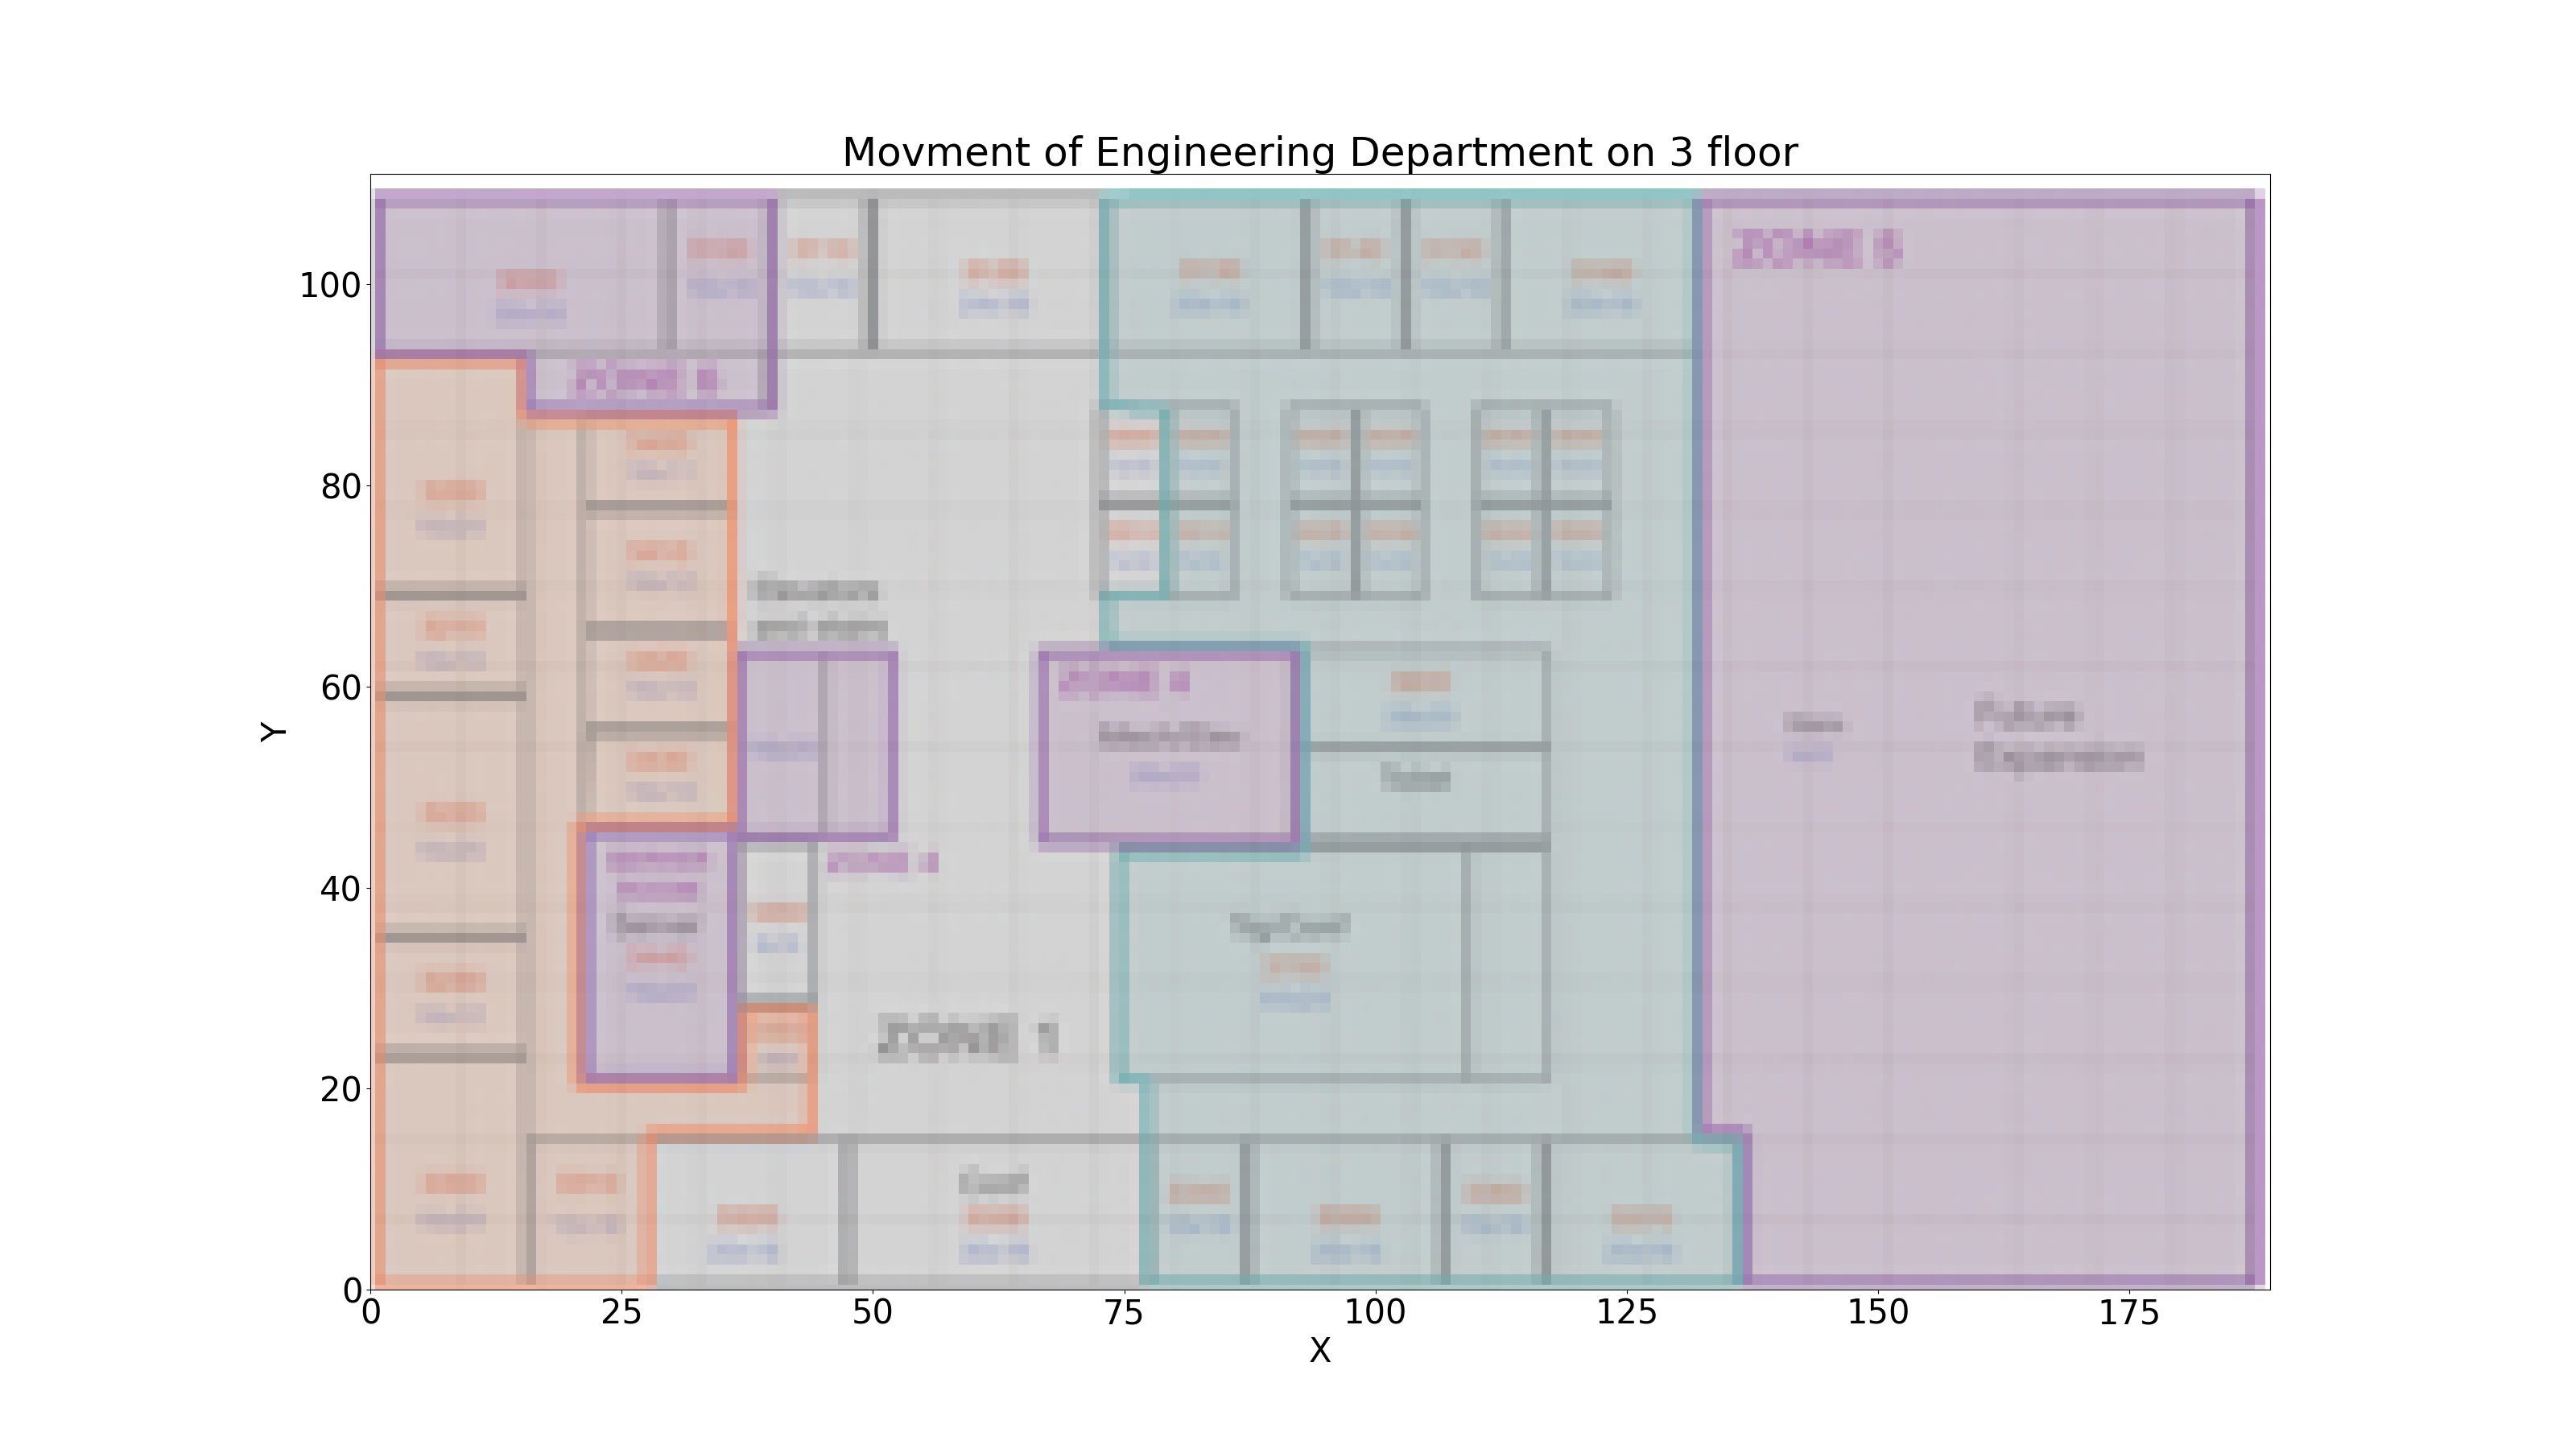
\includegraphics[width=0.3 \linewidth]{figures/Engineering3.png}
                        \\
                        
                        \mbox{(a) First Floor} & \mbox{(b) Second Floor} & \mbox{(c) Third Floor} \\
                    \end{array}$
                    \caption{Movement within Engineering Department}
                    \label{fig:engineering}
                \end{figure}
                
                Secondly, there are distinction layers of movement by department. In the case of the Administration department, as figure \ref{fig:admin}, there was the most movement on the third floor and there was clearly less movement on the second floor. According to the employee data, the administration department has an office in each of floor, so it needs further investigation into why this pattern comes out. In the engineering department, as figure \ref{fig:engineering}, there was a lot of movement on the second floor and nobody went on the third floor. In the case of Executive Department, it moved the most on the third floor and hardly moved on the second floor. The other departments did not have much variation in their movement on each floor. 
                
                Third, we looked at the pattern differences amongst people with many movements and people with few movements.
        
        \subsection[Question 2]{Describe up to five of the most interesting patterns that appear in the building data. Describe what is notable about the pattern and explain its possible significance.}
            \label{sec:question2}
            \subsubsection{General Information of General Building Data}
                First of section \ref{sec:question2}, we should find about the distribution of general building data. With TSNE technique, we can draw the TSNE plot of general building data as figure \ref{fig:tsnegeneral}.
                
                \begin{figure}[htbp]
                    \centering
                    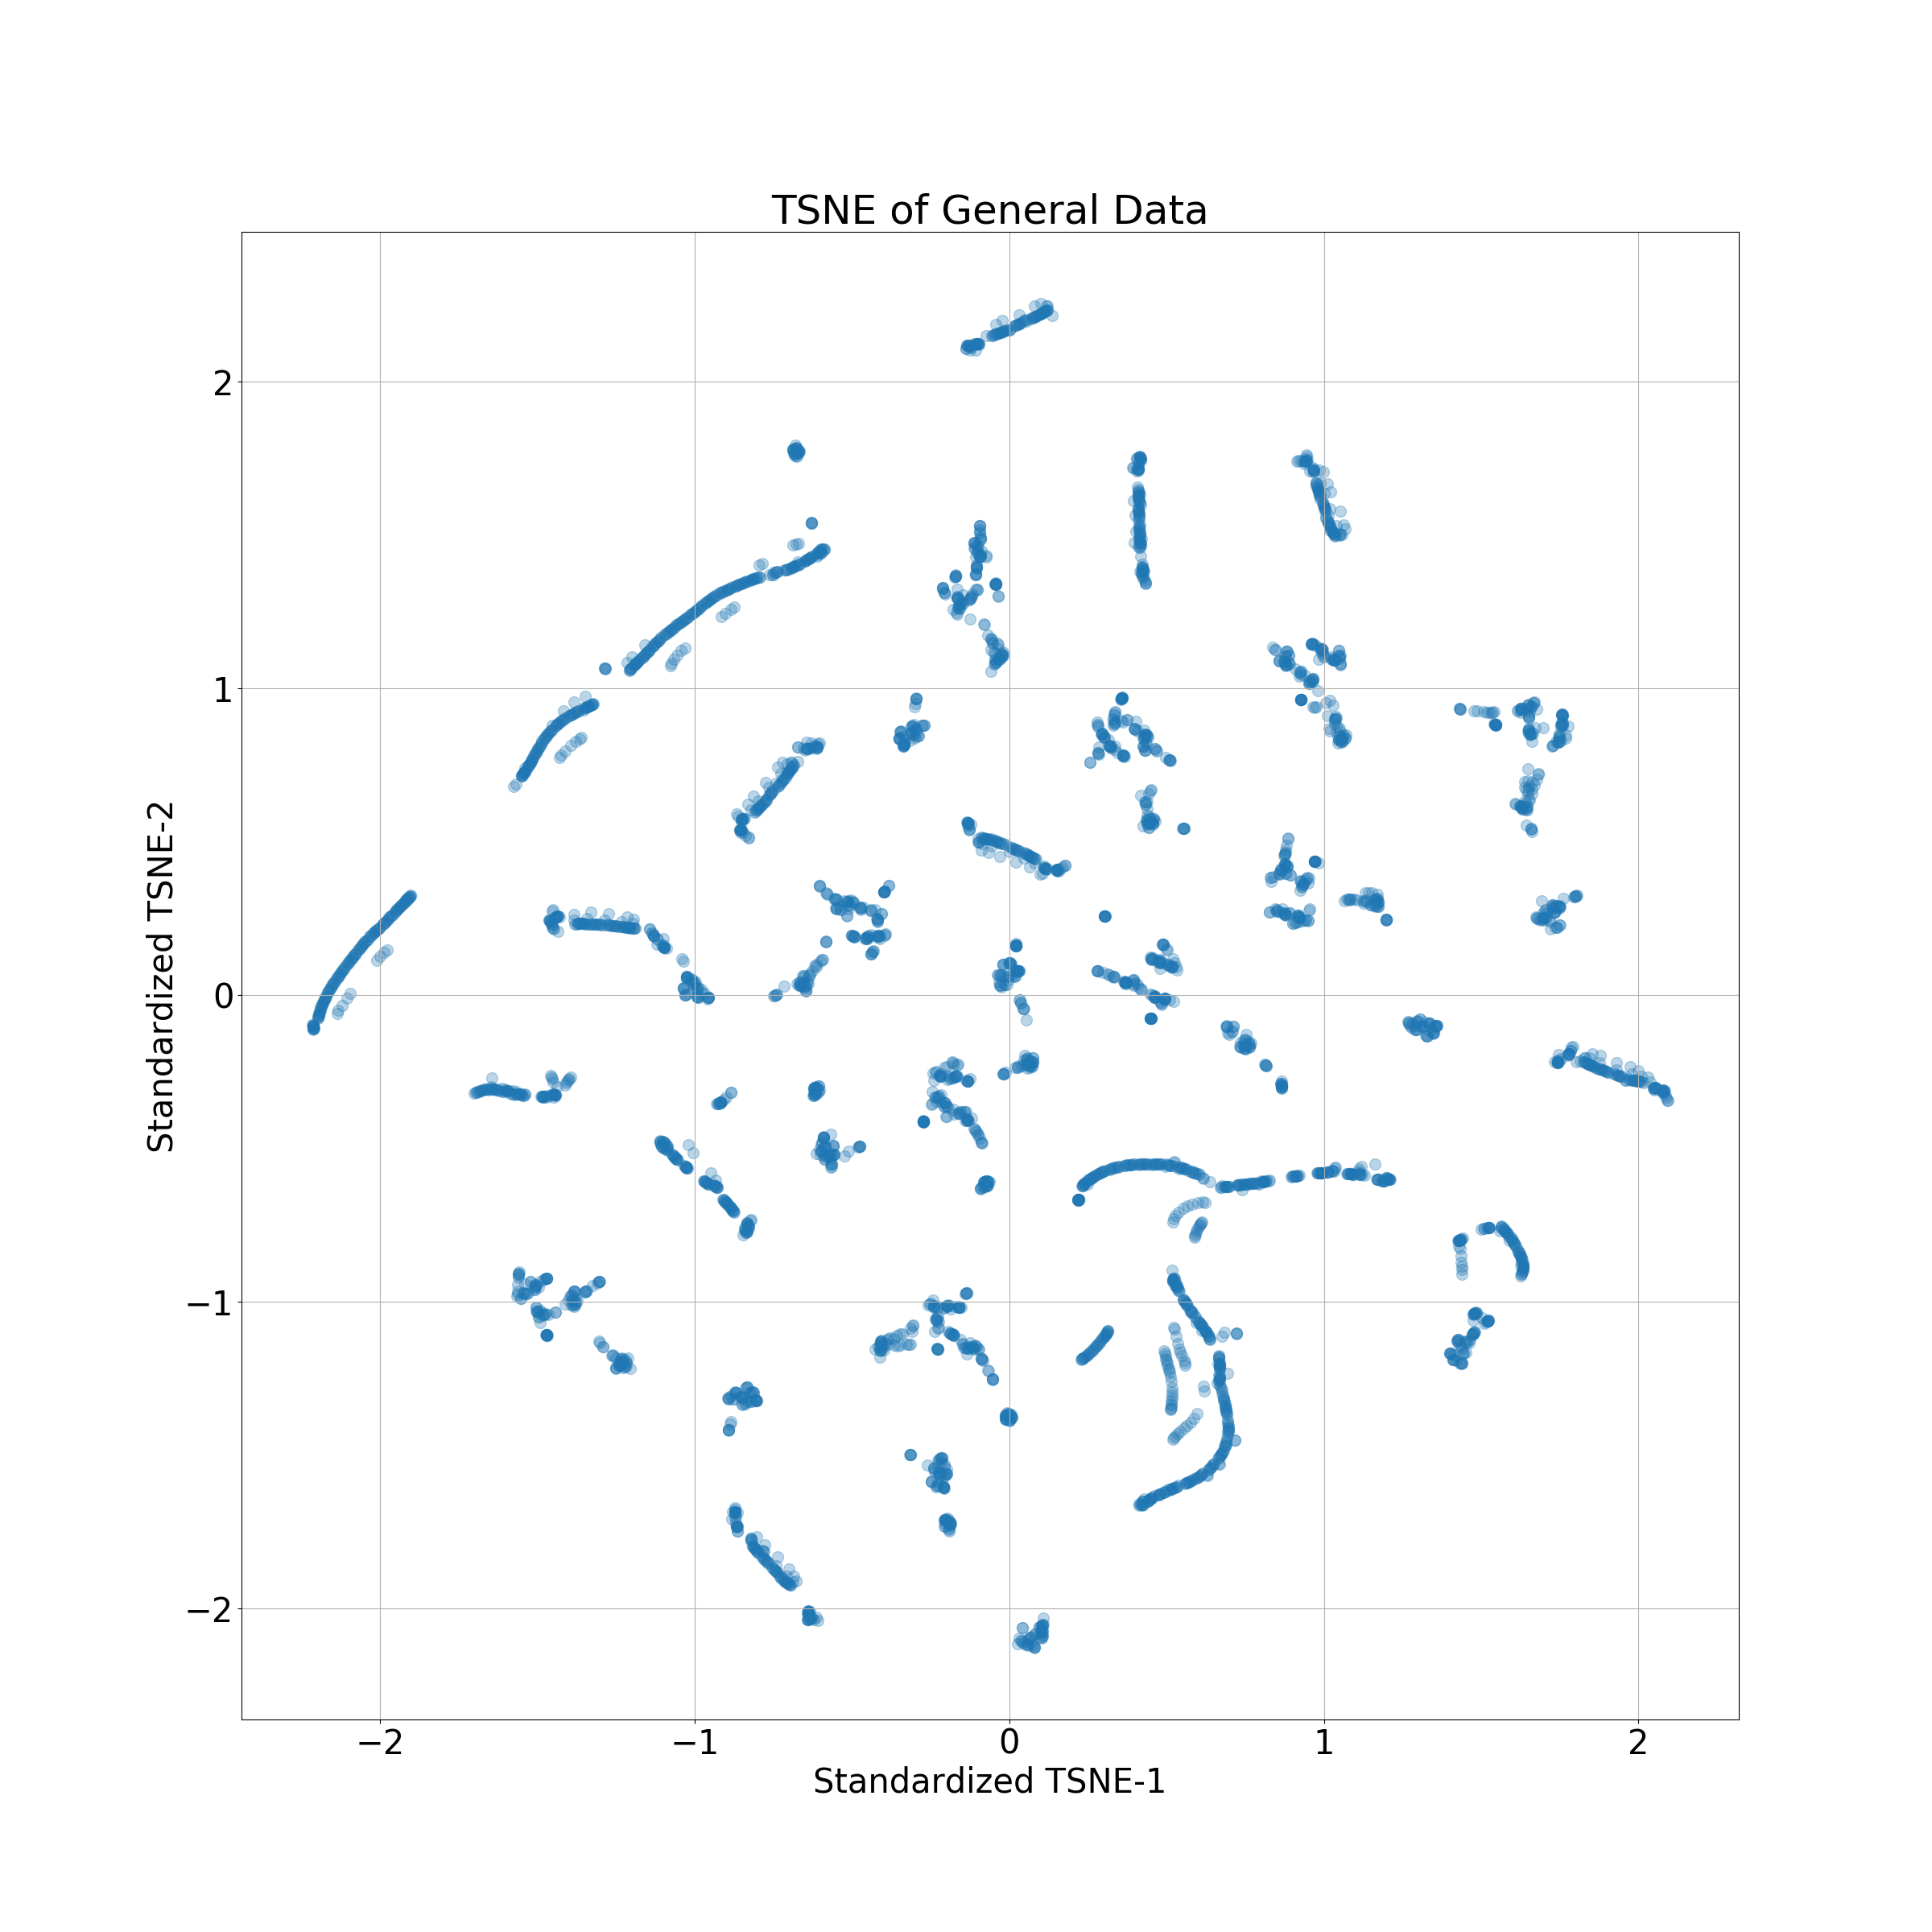
\includegraphics[width=0.4 \linewidth]{figures/TsneGeneral.png}
                    \caption{TSNE for General Building Data}
                    \label{fig:tsnegeneral}
                \end{figure}
            
            \subsubsection{Workflow}
                \begin{figure}[htbp]
                    \centering
                    \begin{tikzpicture}[node distance = 2cm, auto]
                    \end{tikzpicture}
                    \caption{Workflow for Question 2}
                    \label{fig:workflow2}
                \end{figure}
 
            \subsubsection{Correlation within General Building Data} 
                We made the correlation heatmap within the general building data to find two columns which have strong positive or negative correlation. The correlation heatmap is as figure \ref{fig:correlationgeneral}. Moreover, the R-value distribution with the data which are used in figure \ref{fig:correlationgeneral} is as shown as figure \ref{fig:rgeneral}.
                
                \begin{figure}[htbp]
                    \centering
                    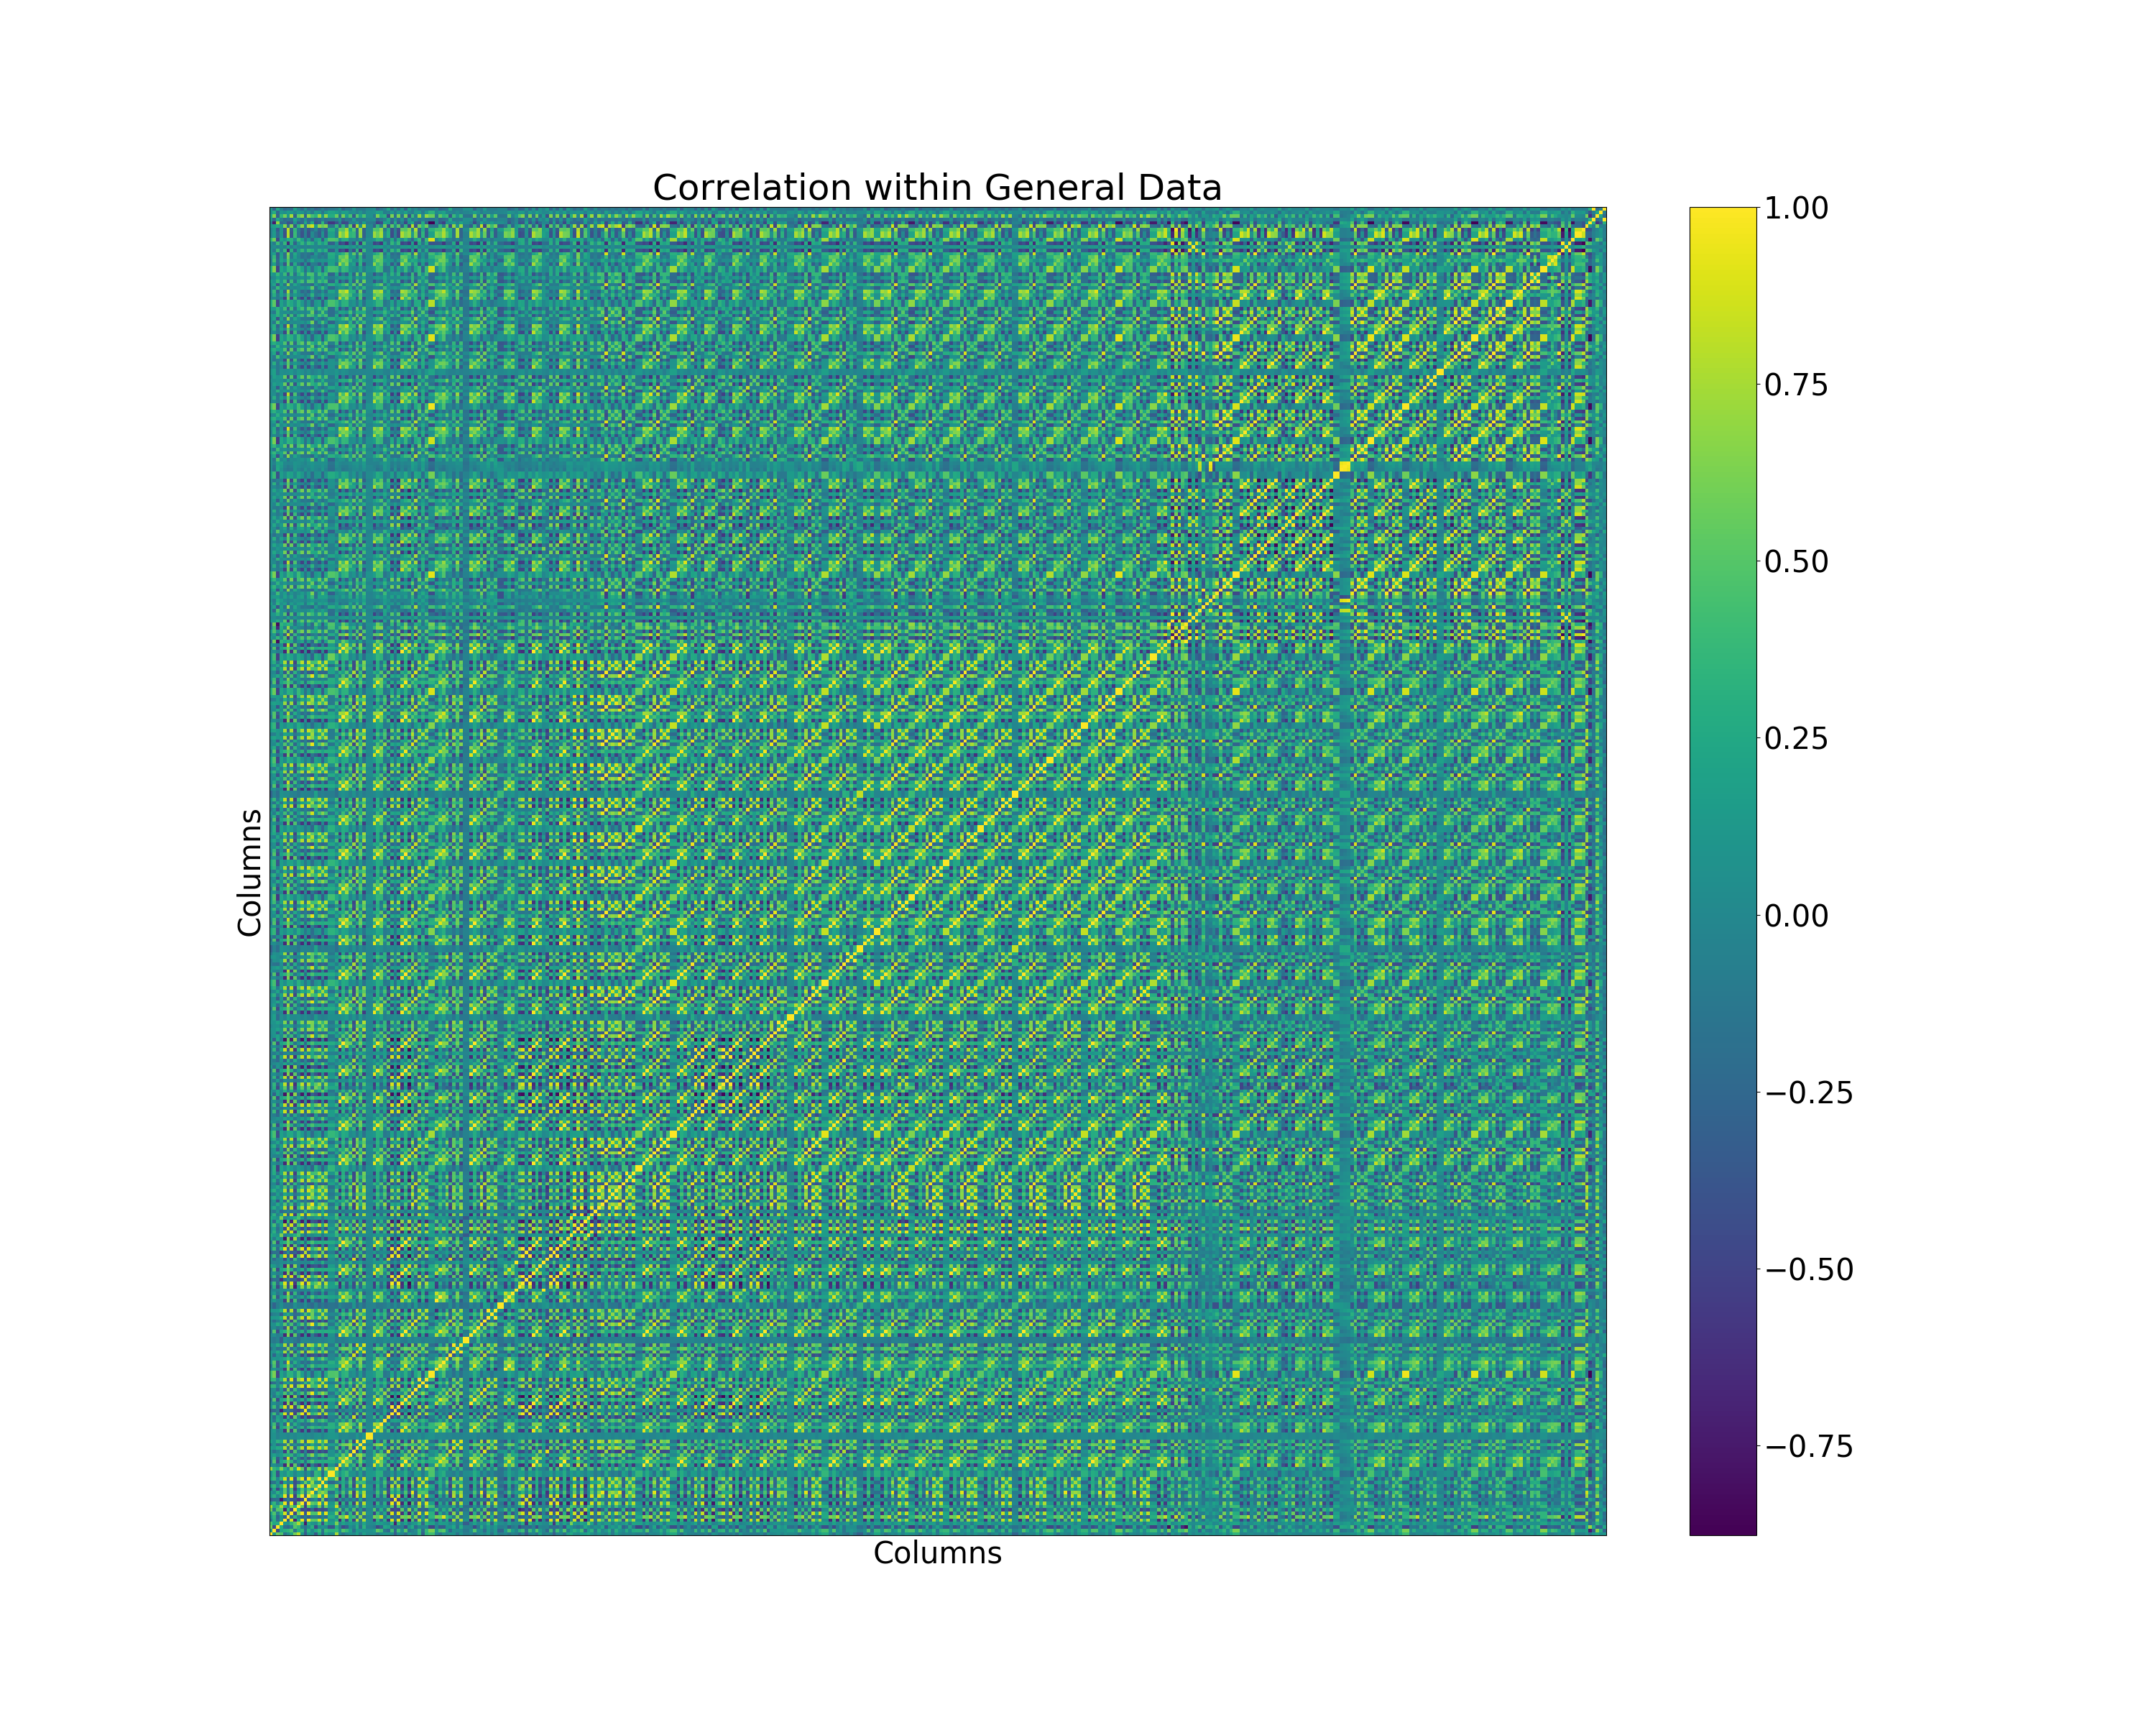
\includegraphics[width=0.4 \linewidth]{figures/correlationgeneral.png}
                    \caption{Correlation Heatmap within General Building Data}
                    \label{fig:correlationgeneral}
                \end{figure}
            
                \begin{figure}[htbp]
                    \centering
                    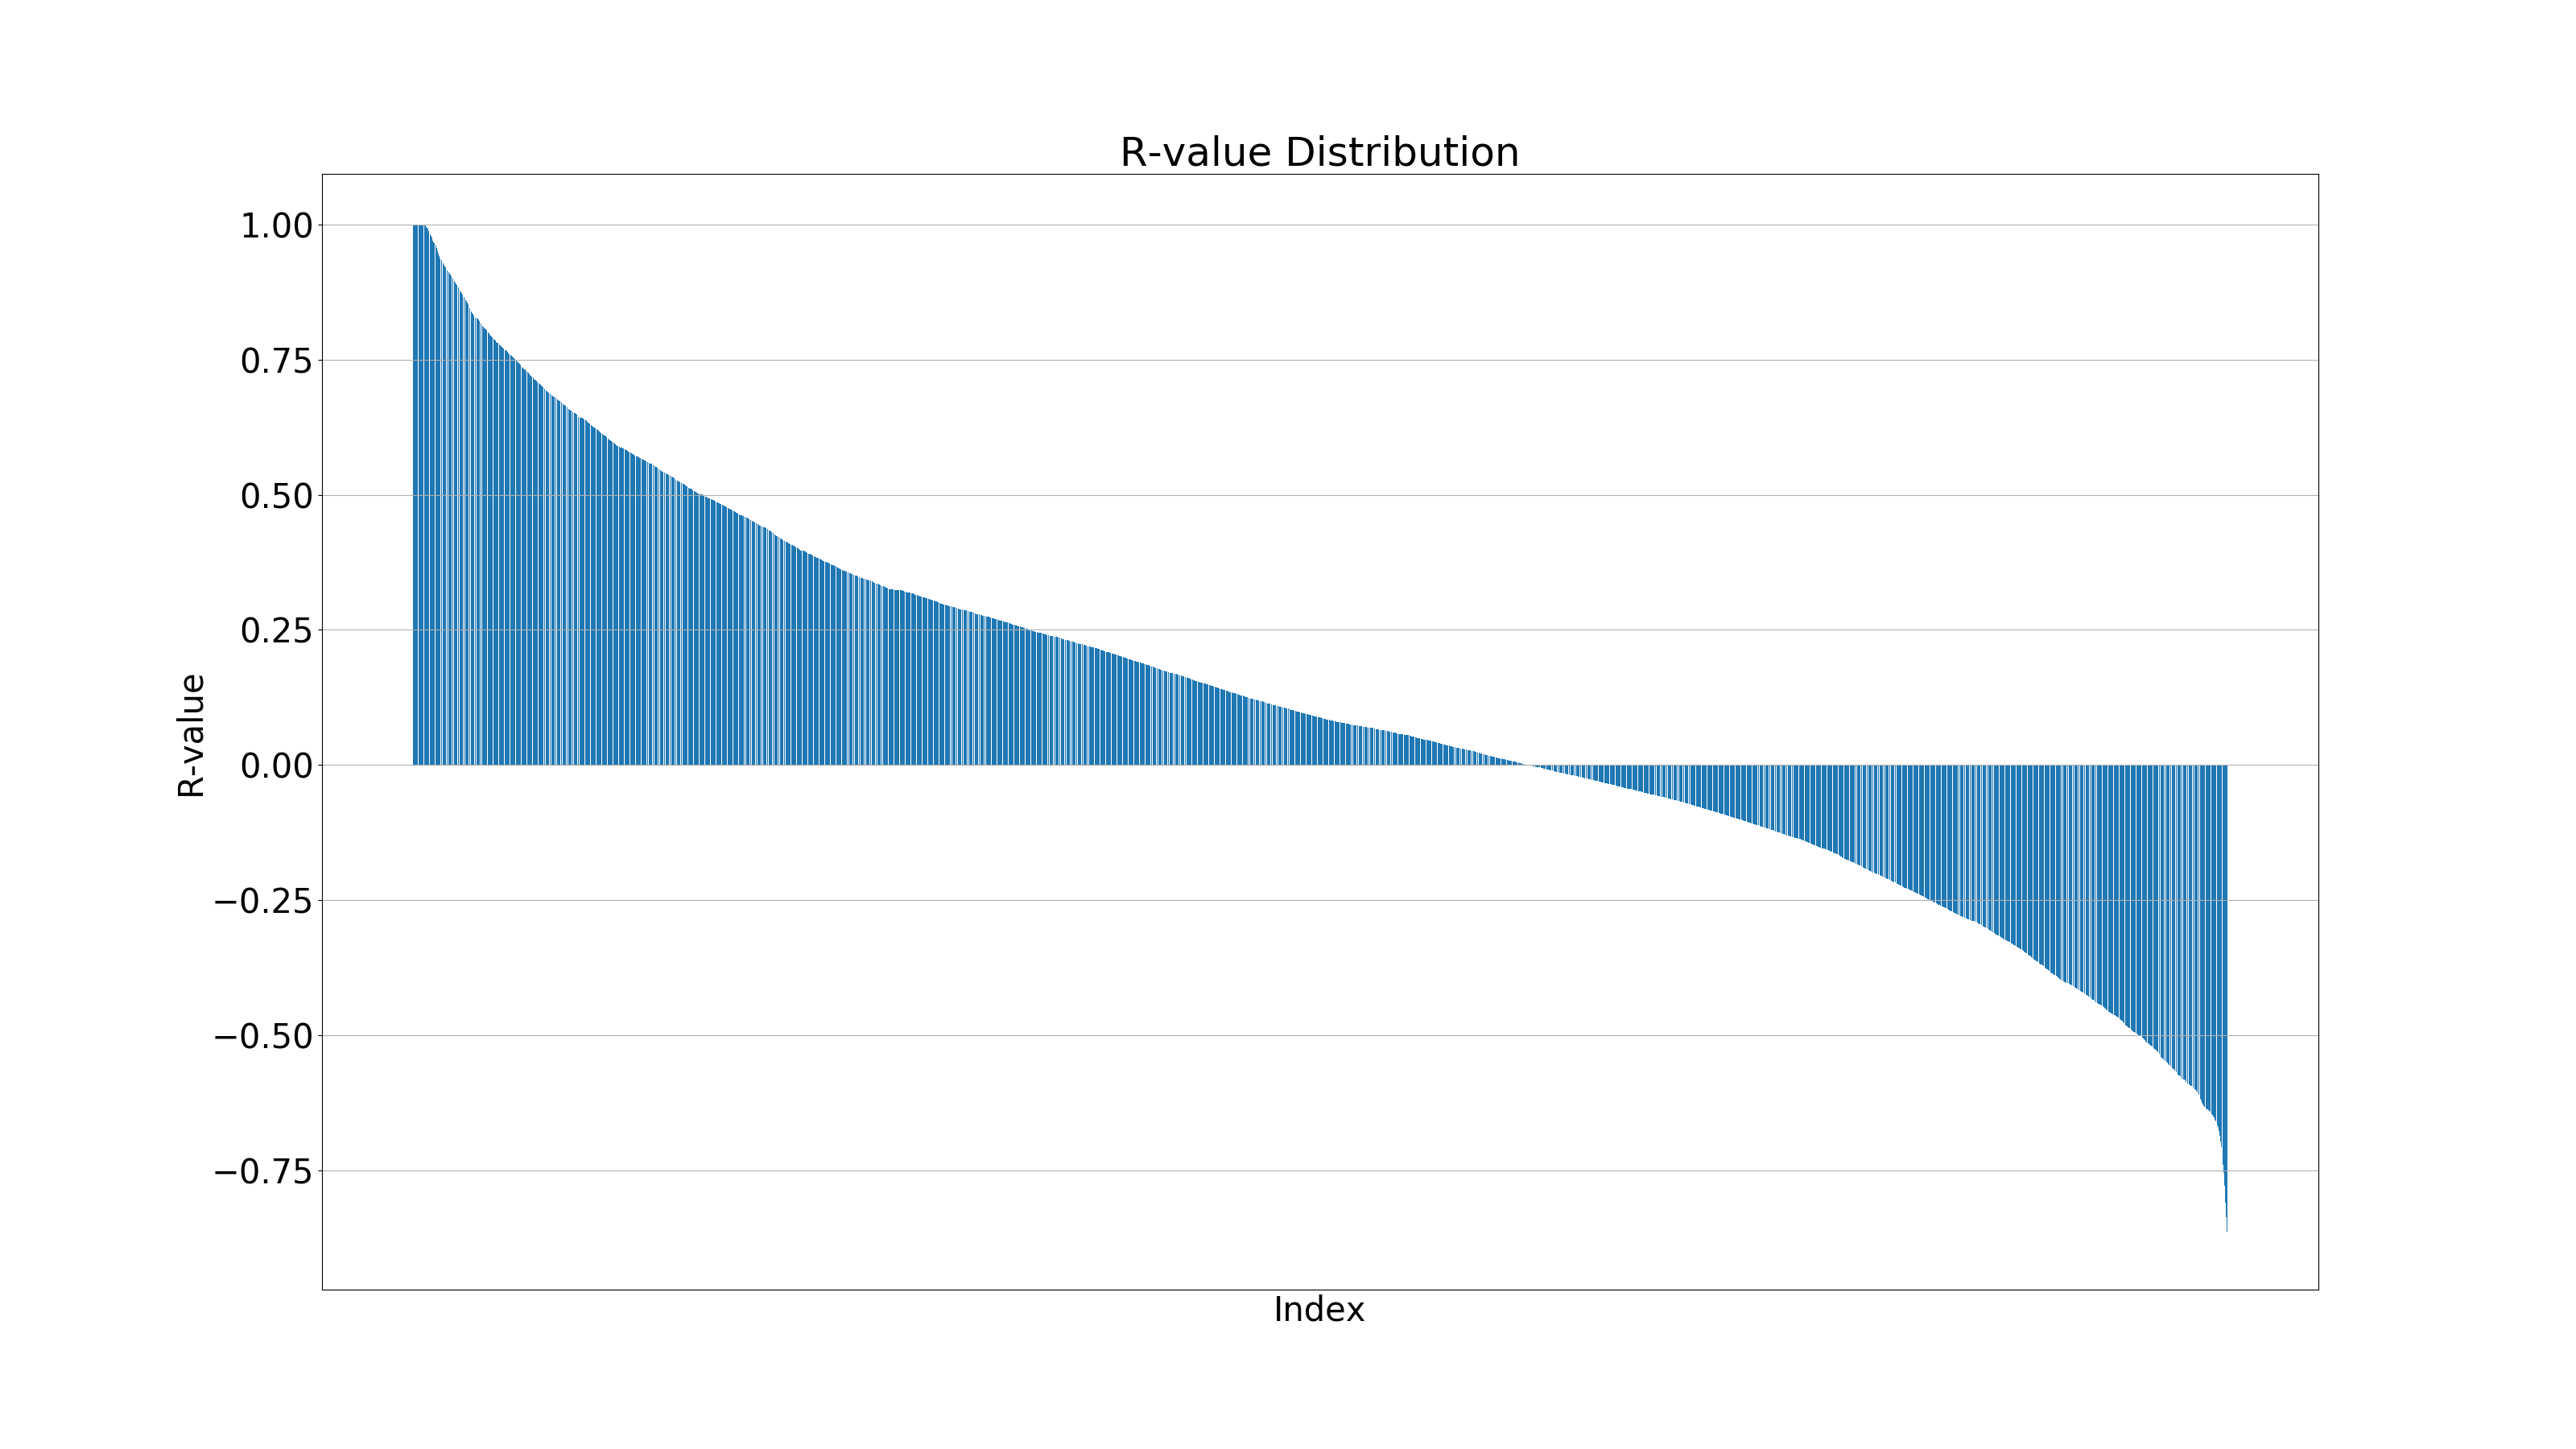
\includegraphics[width=0.5 \linewidth]{figures/rgeneral.png}
                    \caption{R-value Distribution within General Building Data}
                    \label{fig:rgeneral}
                \end{figure}
            
                The basic statistics of these R-values are in table \ref{tb:rgeneral}.
                
                \begin{table}[htbp]
                    \centering
                    \caption{Basic Statistics of R-Values}
                    \label{tb:rgeneral}
                    \begin{tabular}{c||c|c|c|c|c|c|c}
                        Item & Minimum & Maximum & Mean & q1 & Median & q3 & Standard Deviation \\ \hline
                        Value & -0.88 & 1.0 & 0.11 & -0.12 & 0.08 & 0.34 & 0.37 \\
                    \end{tabular}
                \end{table}
            
                Furthermore, the extreme values of R-values are in tables \ref{tb:rmin} and \ref{tb:rmax}.
                
                \begin{table}[htbp]
                    \centering
                    \caption{Minimum Values of R-Values}
                    \label{tb:rmin}
                    \begin{tabular}{c|c||c}
                        Column1 & Column2 & R-Value \\ \hline
                        F\_3\_Z\_11C: Thermostat Temp & F\_3\_Z\_11B VAV REHEAT Damper Position & -0.877076318455652 \\
                        F\_3\_Z\_11C: Thermostat Temp & F\_3\_Z\_11B SUPPLY INLET Mass Flow Rate & -0.8770746421685551 \\
                        Supply Side Inlet Temperature & F\_3\_Z\_6: Equipment Power & -0.8764301266869379 \\
                        Supply Side Inlet Temperature & F\_3\_Z\_6: Lights Power & -0.8764301266869379 \\
                        Supply Side Inlet Temperature & F\_1\_Z\_4: Lights Power & -0.8743564507417133 \\
                    \end{tabular}
                \end{table}
            
                \begin{table}[htbp]
                    \centering
                    \caption{Maximum Values of R-Values}
                    \label{tb:rmax}
                    \begin{tabular}{c|c||c}
                        Column1 & Column2 & R-Value \\ \hline
                        Water Heater Tank Temperature & Supply Side Outlet Temperature & 1.0 \\
                        F\_3\_Z\_7: Thermostat Heating Setpoint & F\_3\_Z\_3: Thermostat Heating Setpoint & 1.0 \\
                        F\_3\_Z\_7: Thermostat Heating Setpoint & F\_3\_Z\_2: Thermostat Heating Setpoint & 1.0 \\
                        F\_3\_Z\_7: Thermostat Heating Setpoint & F\_3\_Z\_11B: Thermostat Heating Setpoint & 1.0 \\
                        F\_3\_Z\_7: Thermostat Heating Setpoint & F\_3\_Z\_11A: Thermostat Heating Setpoint & 1.0 \\
                        F\_3\_Z\_7: Thermostat Heating Setpoint & F\_3\_Z\_10: Thermostat Heating Setpoint & 1.0 \\
                        F\_3\_Z\_7: Thermostat Cooling Setpoint & F\_3\_Z\_3: Thermostat Cooling Setpoint & 1.0 \\
                        F\_3\_Z\_7: Thermostat Cooling Setpoint & F\_3\_Z\_2: Thermostat Cooling Setpoint & 1.0 \\
                        F\_3\_Z\_7: Thermostat Cooling Setpoint & F\_3\_Z\_11B: Thermostat Cooling Setpoint & 1.0 \\
                        F\_3\_Z\_7: Thermostat Cooling Setpoint & F\_3\_Z\_11A: Thermostat Cooling Setpoint & 1.0 \\
                        F\_3\_Z\_7: Thermostat Cooling Setpoint & F\_3\_Z\_10: Thermostat Cooling Setpoint & 1.0 \\
                        F\_3\_Z\_6: Thermostat Heating Setpoint & F\_3\_Z\_5: Thermostat Heating Setpoint & 1.0 \\
                        F\_3\_Z\_6: Thermostat Cooling Setpoint & F\_3\_Z\_5: Thermostat Cooling Setpoint & 1.0 \\
                        F\_3\_Z\_6: Lights Power & F\_3\_Z\_6: Equipment Power & 1.0 \\
                        F\_3\_Z\_5: Lights Power & F\_3\_Z\_5: Equipment Power & 1.0 \\
                        F\_3\_Z\_3: Thermostat Heating Setpoint & F\_3\_Z\_2: Thermostat Heating Setpoint & 1.0 \\
                        F\_3\_Z\_3: Thermostat Heating Setpoint & F\_3\_Z\_11B: Thermostat Heating Setpoint & 1.0 \\
                        F\_3\_Z\_3: Thermostat Heating Setpoint & F\_3\_Z\_11A: Thermostat Heating Setpoint & 1.0 \\
                        F\_3\_Z\_3: Thermostat Heating Setpoint & F\_3\_Z\_10: Thermostat Heating Setpoint & 1.0 \\
                        F\_3\_Z\_3: Thermostat Cooling Setpoint & F\_3\_Z\_2: Thermostat Cooling Setpoint & 1.0 \\
                        F\_3\_Z\_3: Thermostat Cooling Setpoint & F\_3\_Z\_11B: Thermostat Cooling Setpoint & 1.0 \\
                        F\_3\_Z\_3: Thermostat Cooling Setpoint & F\_3\_Z\_11A: Thermostat Cooling Setpoint & 1.0 \\
                        F\_3\_Z\_3: Thermostat Cooling Setpoint & F\_3\_Z\_10: Thermostat Cooling Setpoint & 1.0 \\
                        F\_3\_Z\_3: Lights Power & F\_3\_Z\_3: Equipment Power & 1.0 \\
                        (omitted...) & (omitted...) &  (omitted...) \\
                    \end{tabular}
                \end{table}
                
                As table \ref{tb:rmin}, no combination of columns make R-value to -1;  but, there are many combinations of columns make R-value 1. In other words, many columns have strong positive correlation with others rather than negative correlation. However, in table \ref{tb:rmax}, most of combination are (Thermostat Heating Setpoint), (Thermostat Cooling Setpoint), or (Lights Power \& Equipment power). Also, not all Thermostat Setpoints in same floor have strong correlation; but, Thermostat Setpoints in different floor do not have strong correlation. 
            
                Furthermore, we draw plot between three general building data which have the lowest R-values as figure \ref{fig:lowest}. In the figure \ref{fig:lowest}, the R-values are about 0.88, so the R-squared values (\( R ^ 2 \)) will be about 0.77. Therefore, in figure \ref{fig:lowest}, we can argue that they have negative correlation, but it is not \textit{strong} negative correlation. 
                
                \begin{figure}[htbp]
                    \centering
                    $\begin{array}{ccc}
                        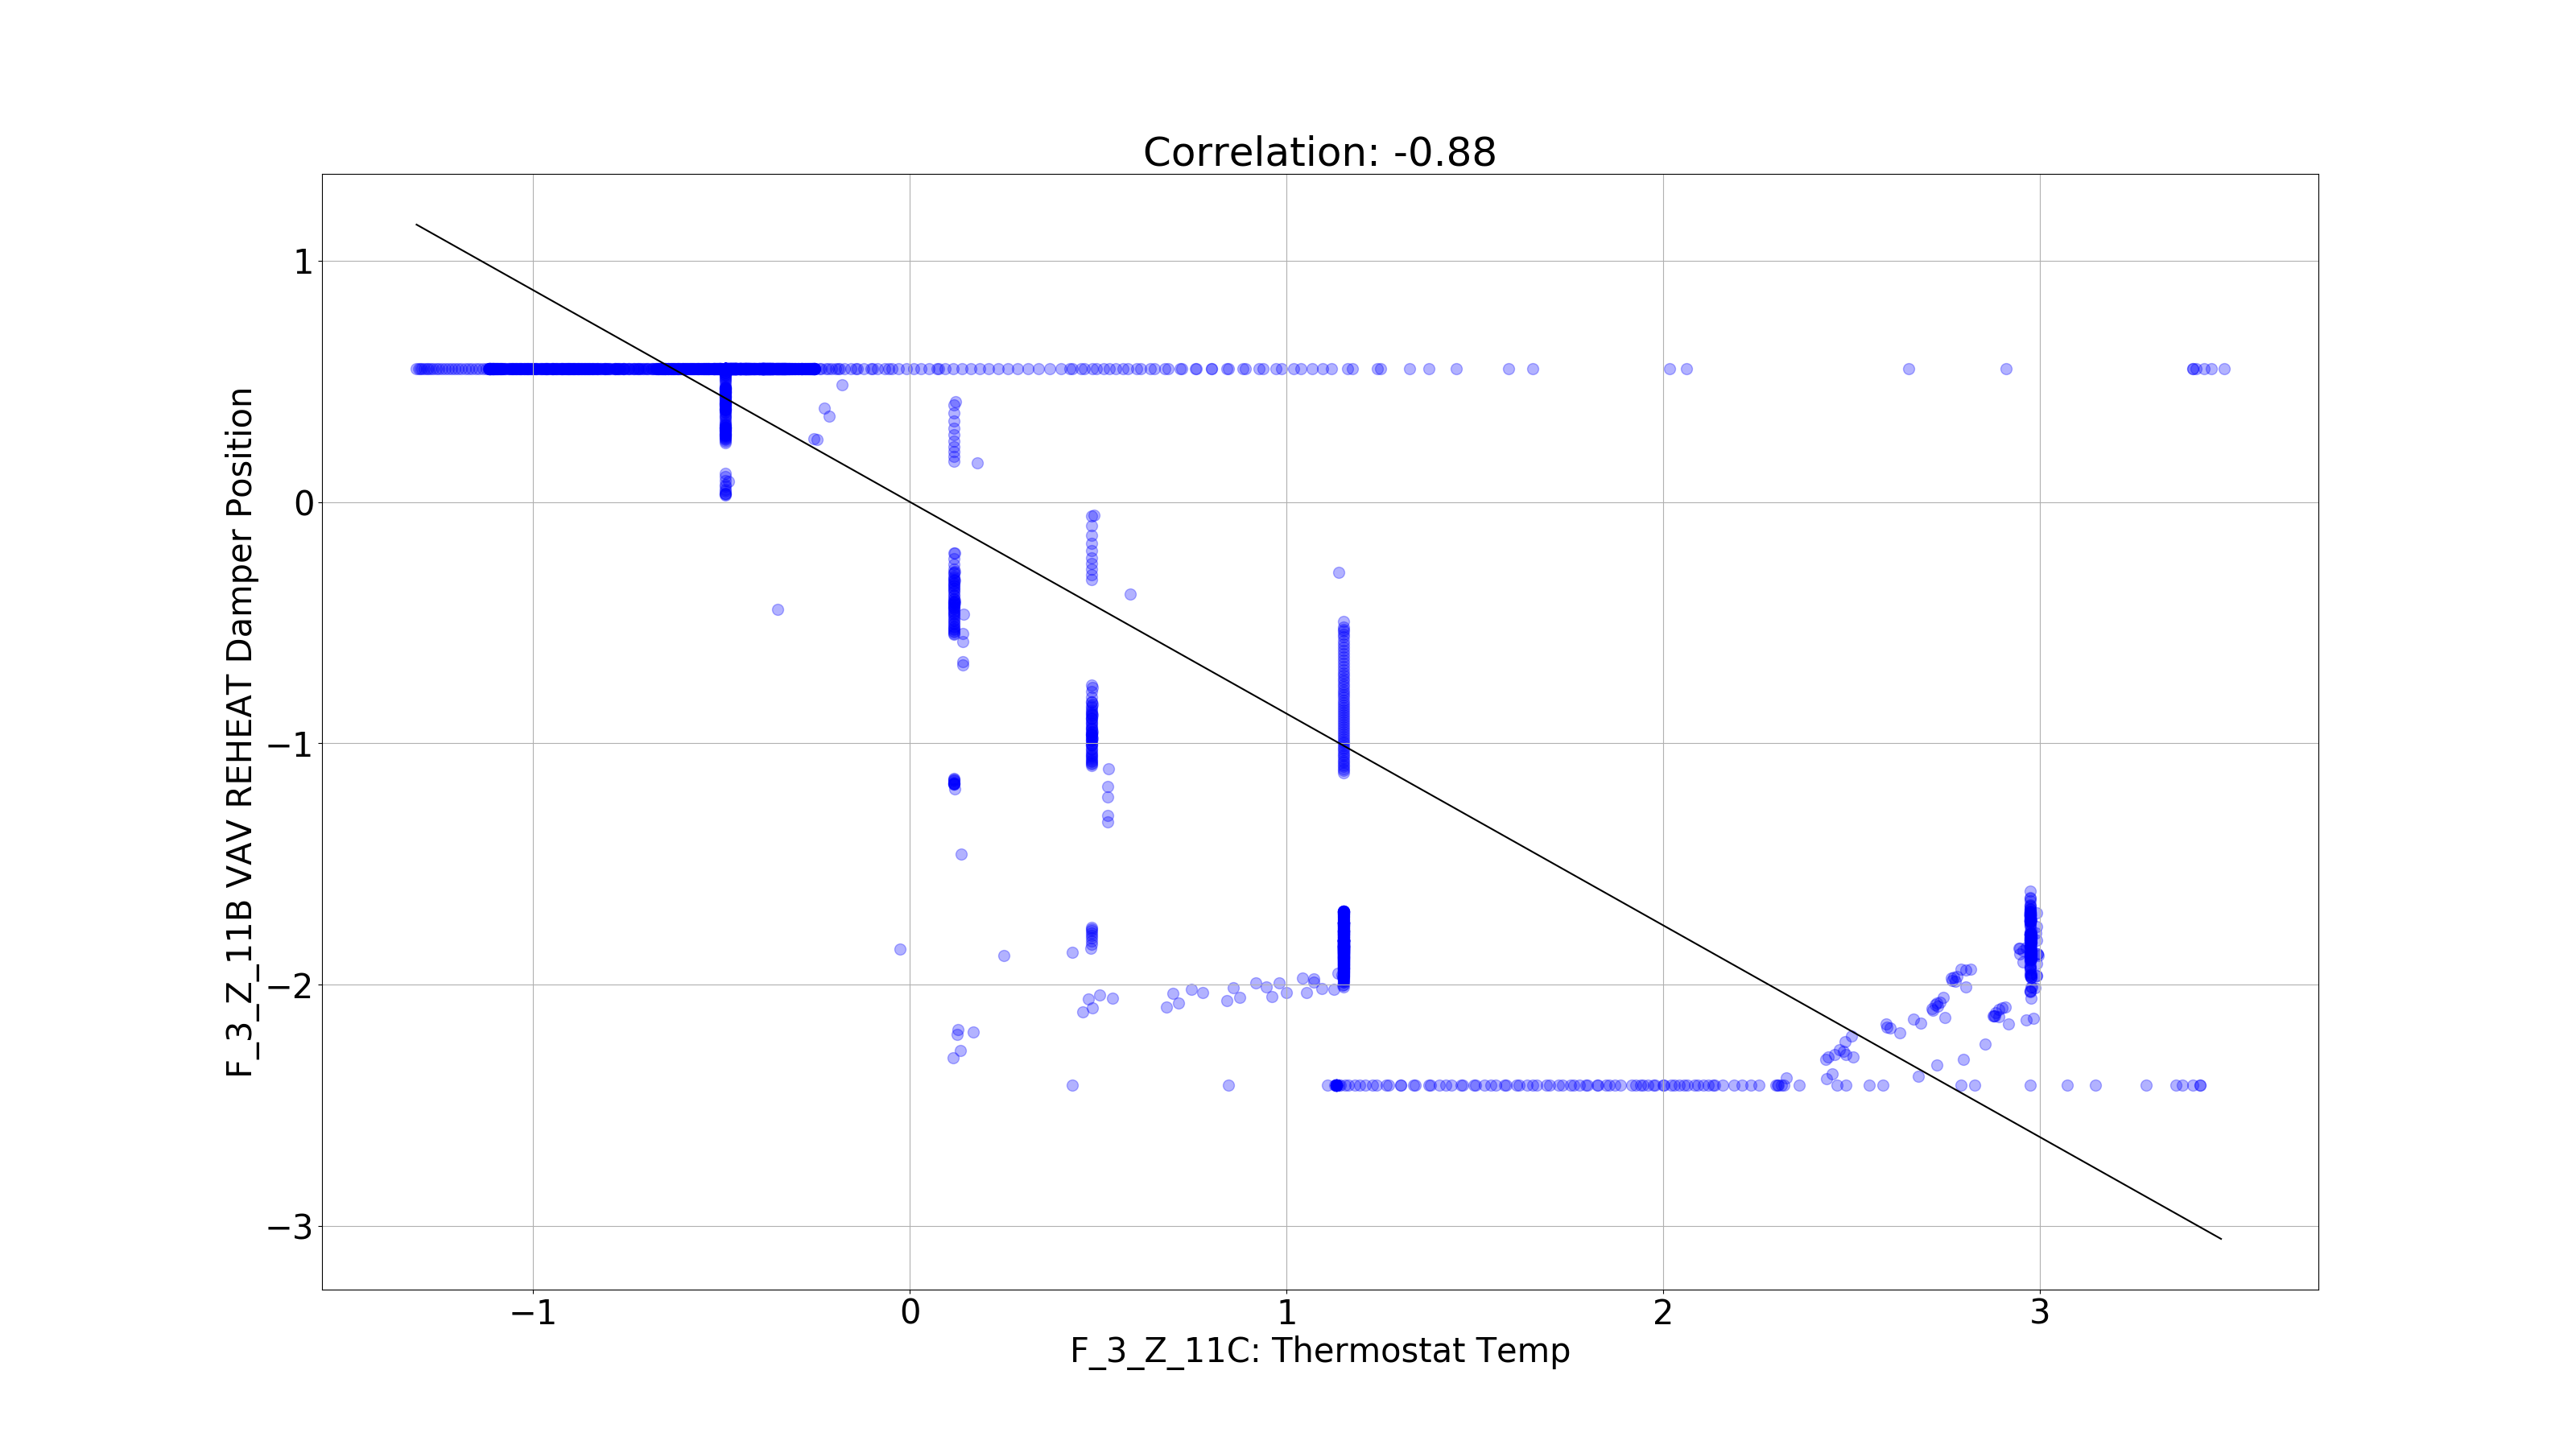
\includegraphics[width=0.3 \linewidth]{Figures/negative1.png}
                        &
                        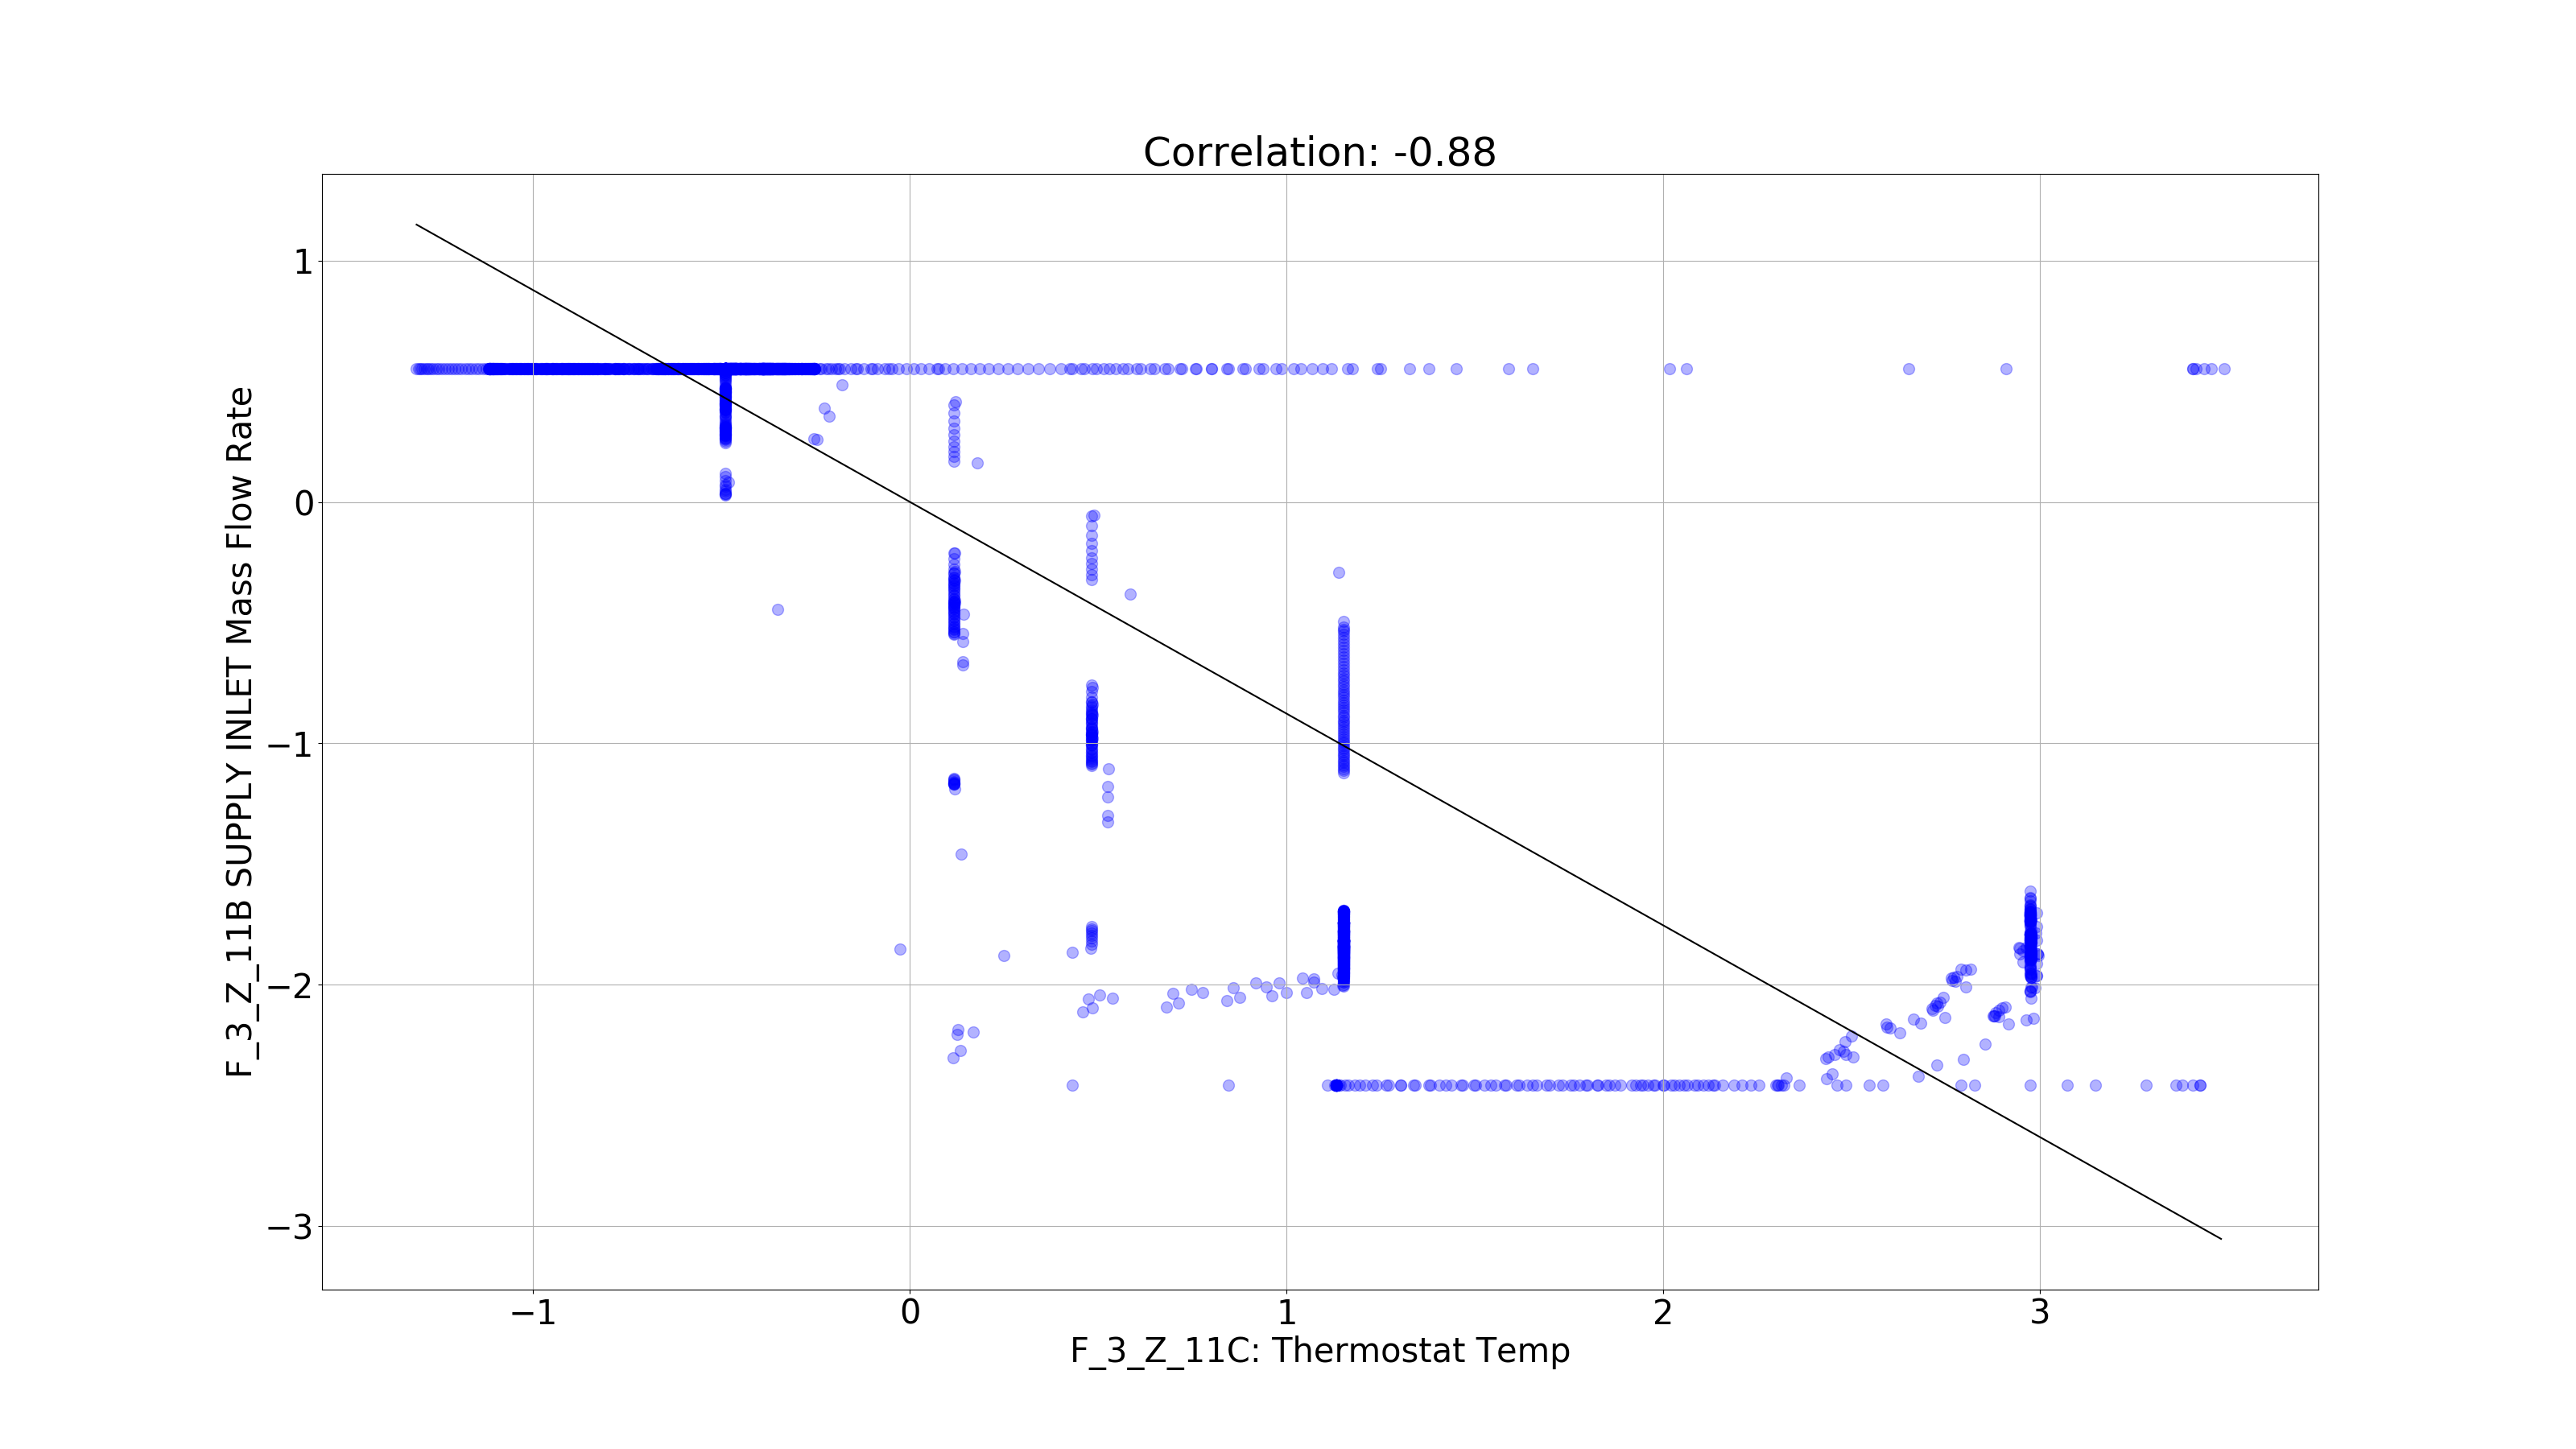
\includegraphics[width=0.3 \linewidth]{Figures/negative2.png}
                        &
                        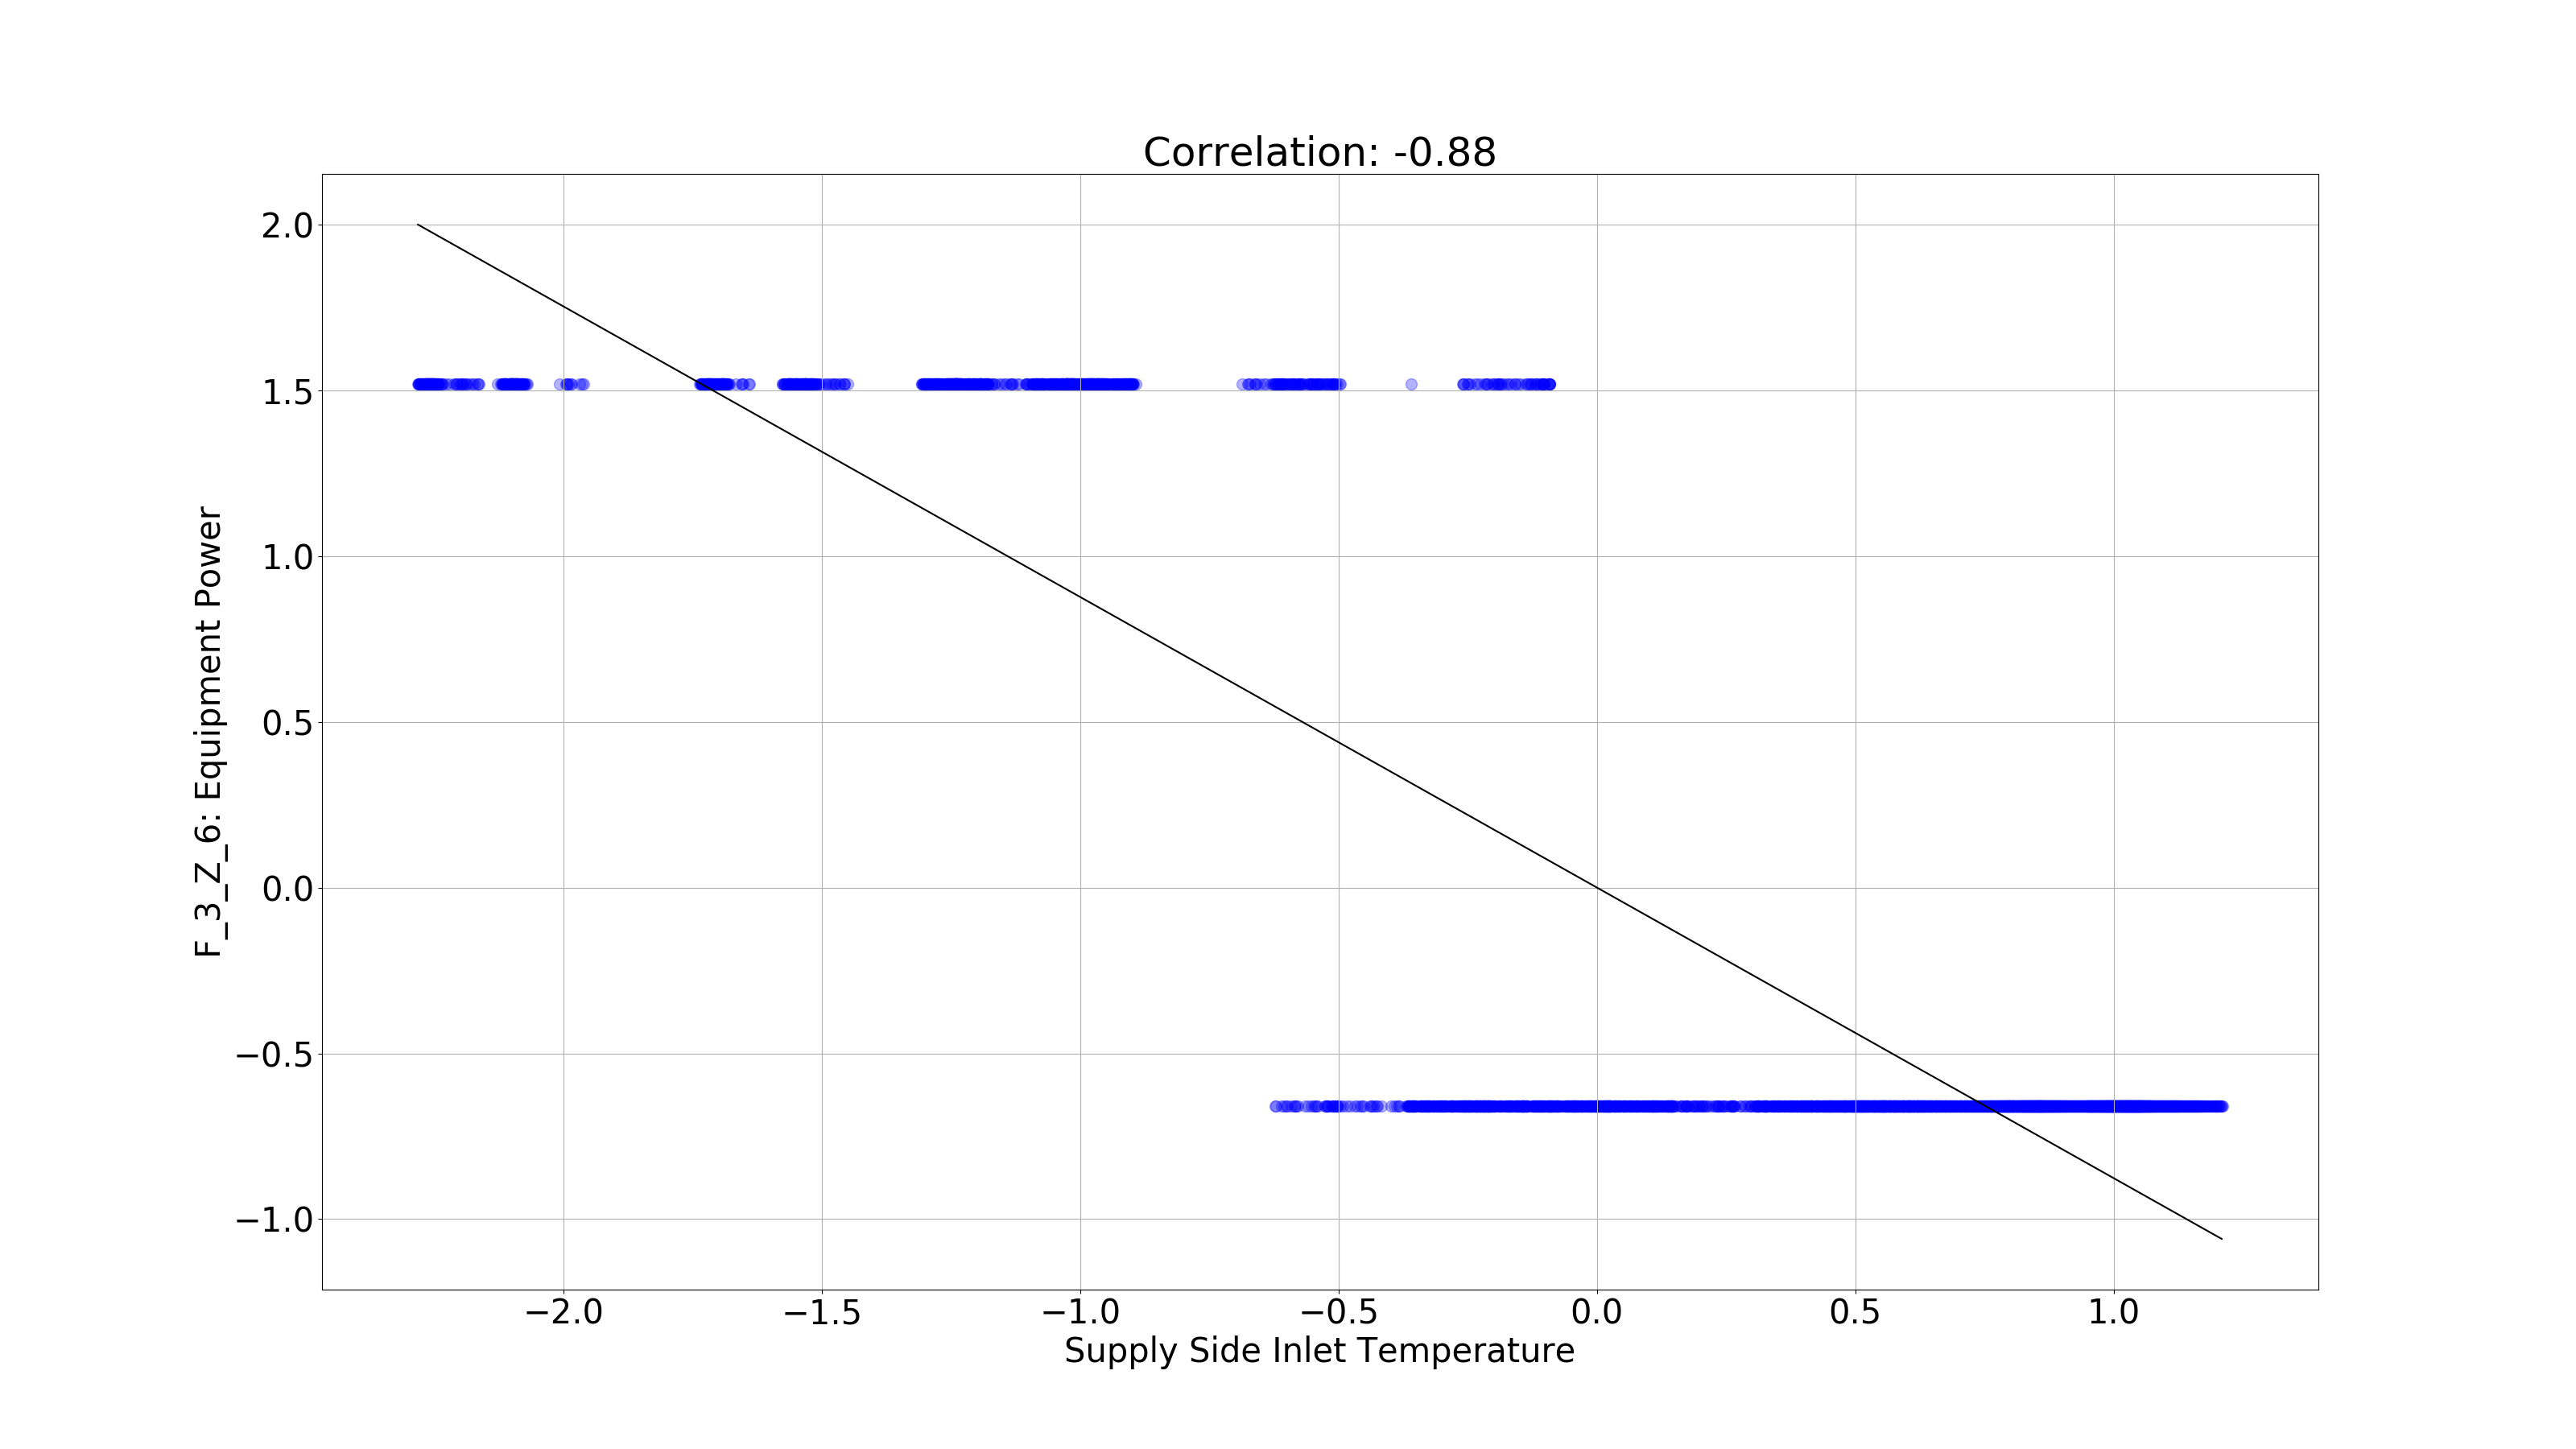
\includegraphics[width=0.3 \linewidth]{Figures/negative3.png}
                        \\
                        \mbox{(a) First} & \mbox{(b) Second} & \mbox{(c) Third} \\
                    \end{array}$
                    \caption{Plots of the Lowest R-values}
                    \label{fig:lowest}
                \end{figure}
                
            \subsubsection{Plots of General Building Data}
                In the figure \ref{fig:general}, there are two plots: Figure \ref{fig:general}-(a) is stacked plot about all columns, and figure \ref{fig:general}-(b) has basic statistics plot of general building data. In figure \ref{fig:general}-(b), we can see that the pattern of general building data is changing by quarters: in first-quarters, the cyclic pattern is shown; in second-quarters, rapidly increasing can be detected; in third-quarters, many general building data jump and hold a while; and, in fourth-quarters, general building data are suddenly decreasing. 
            
                \begin{figure}[htbp]
                    \centering
                    $\begin{array}{cc}
                        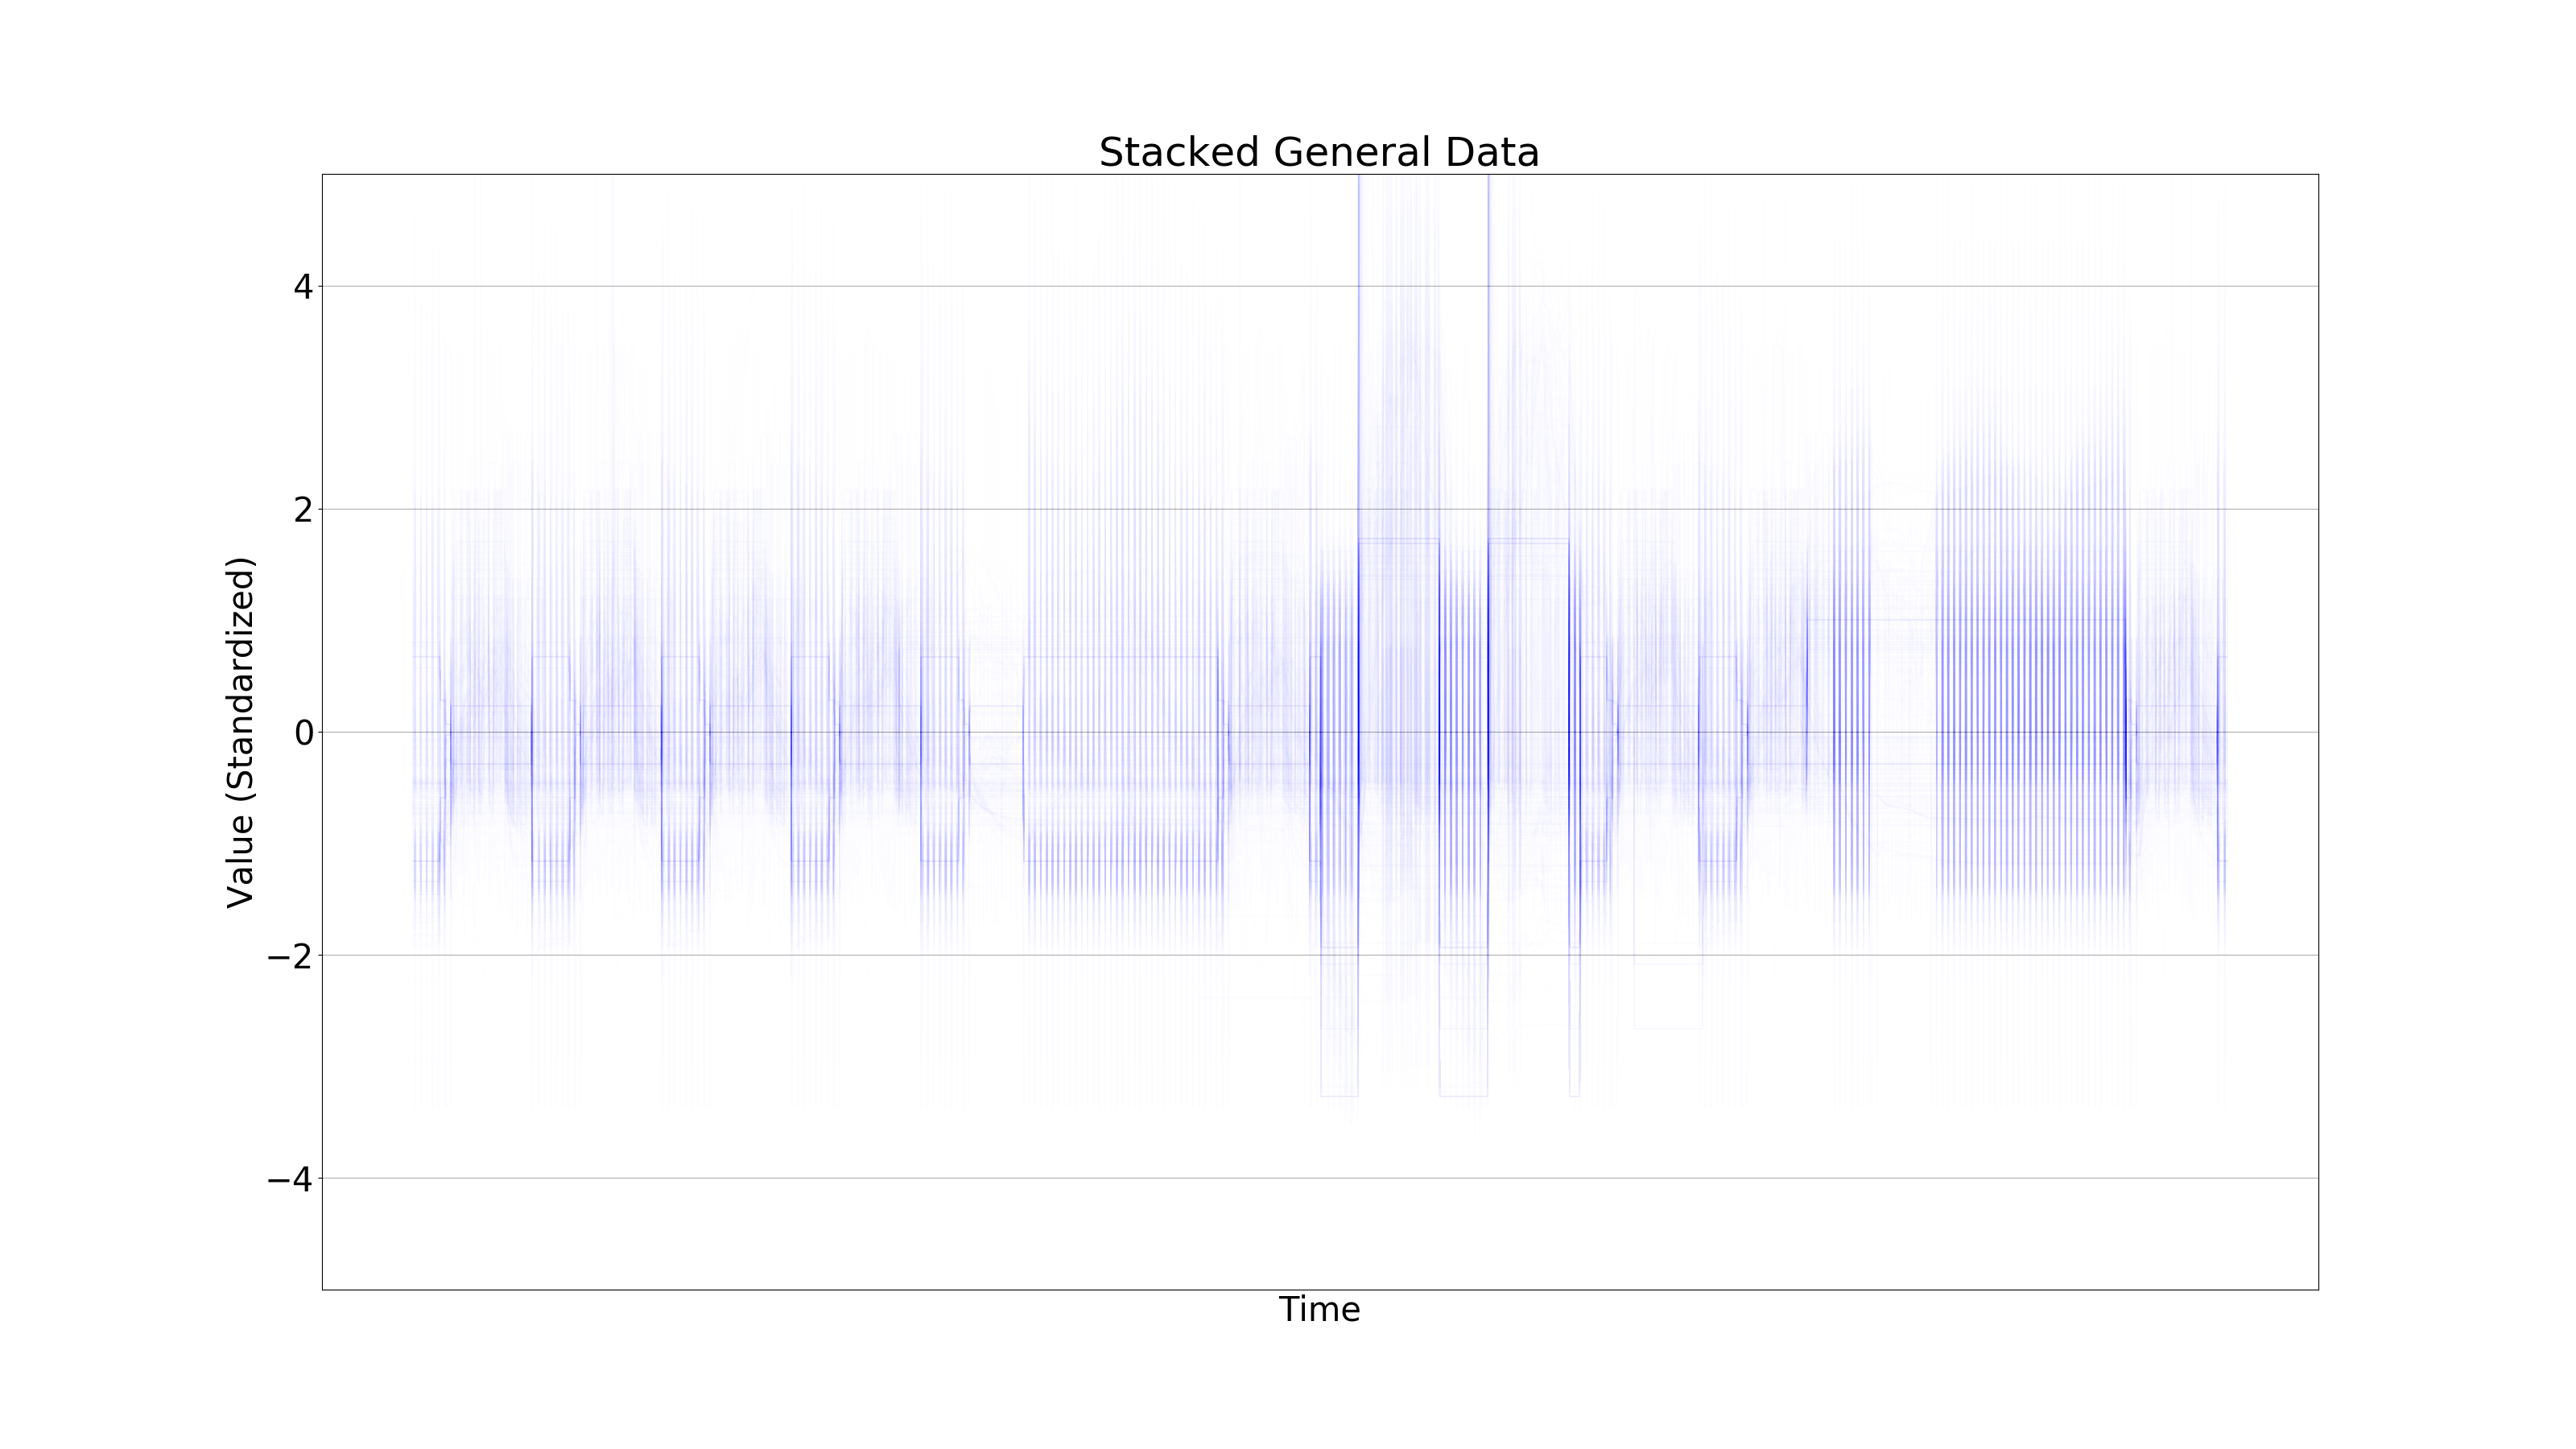
\includegraphics[width=0.4 \linewidth]{figures/general1.png}
                        &
                        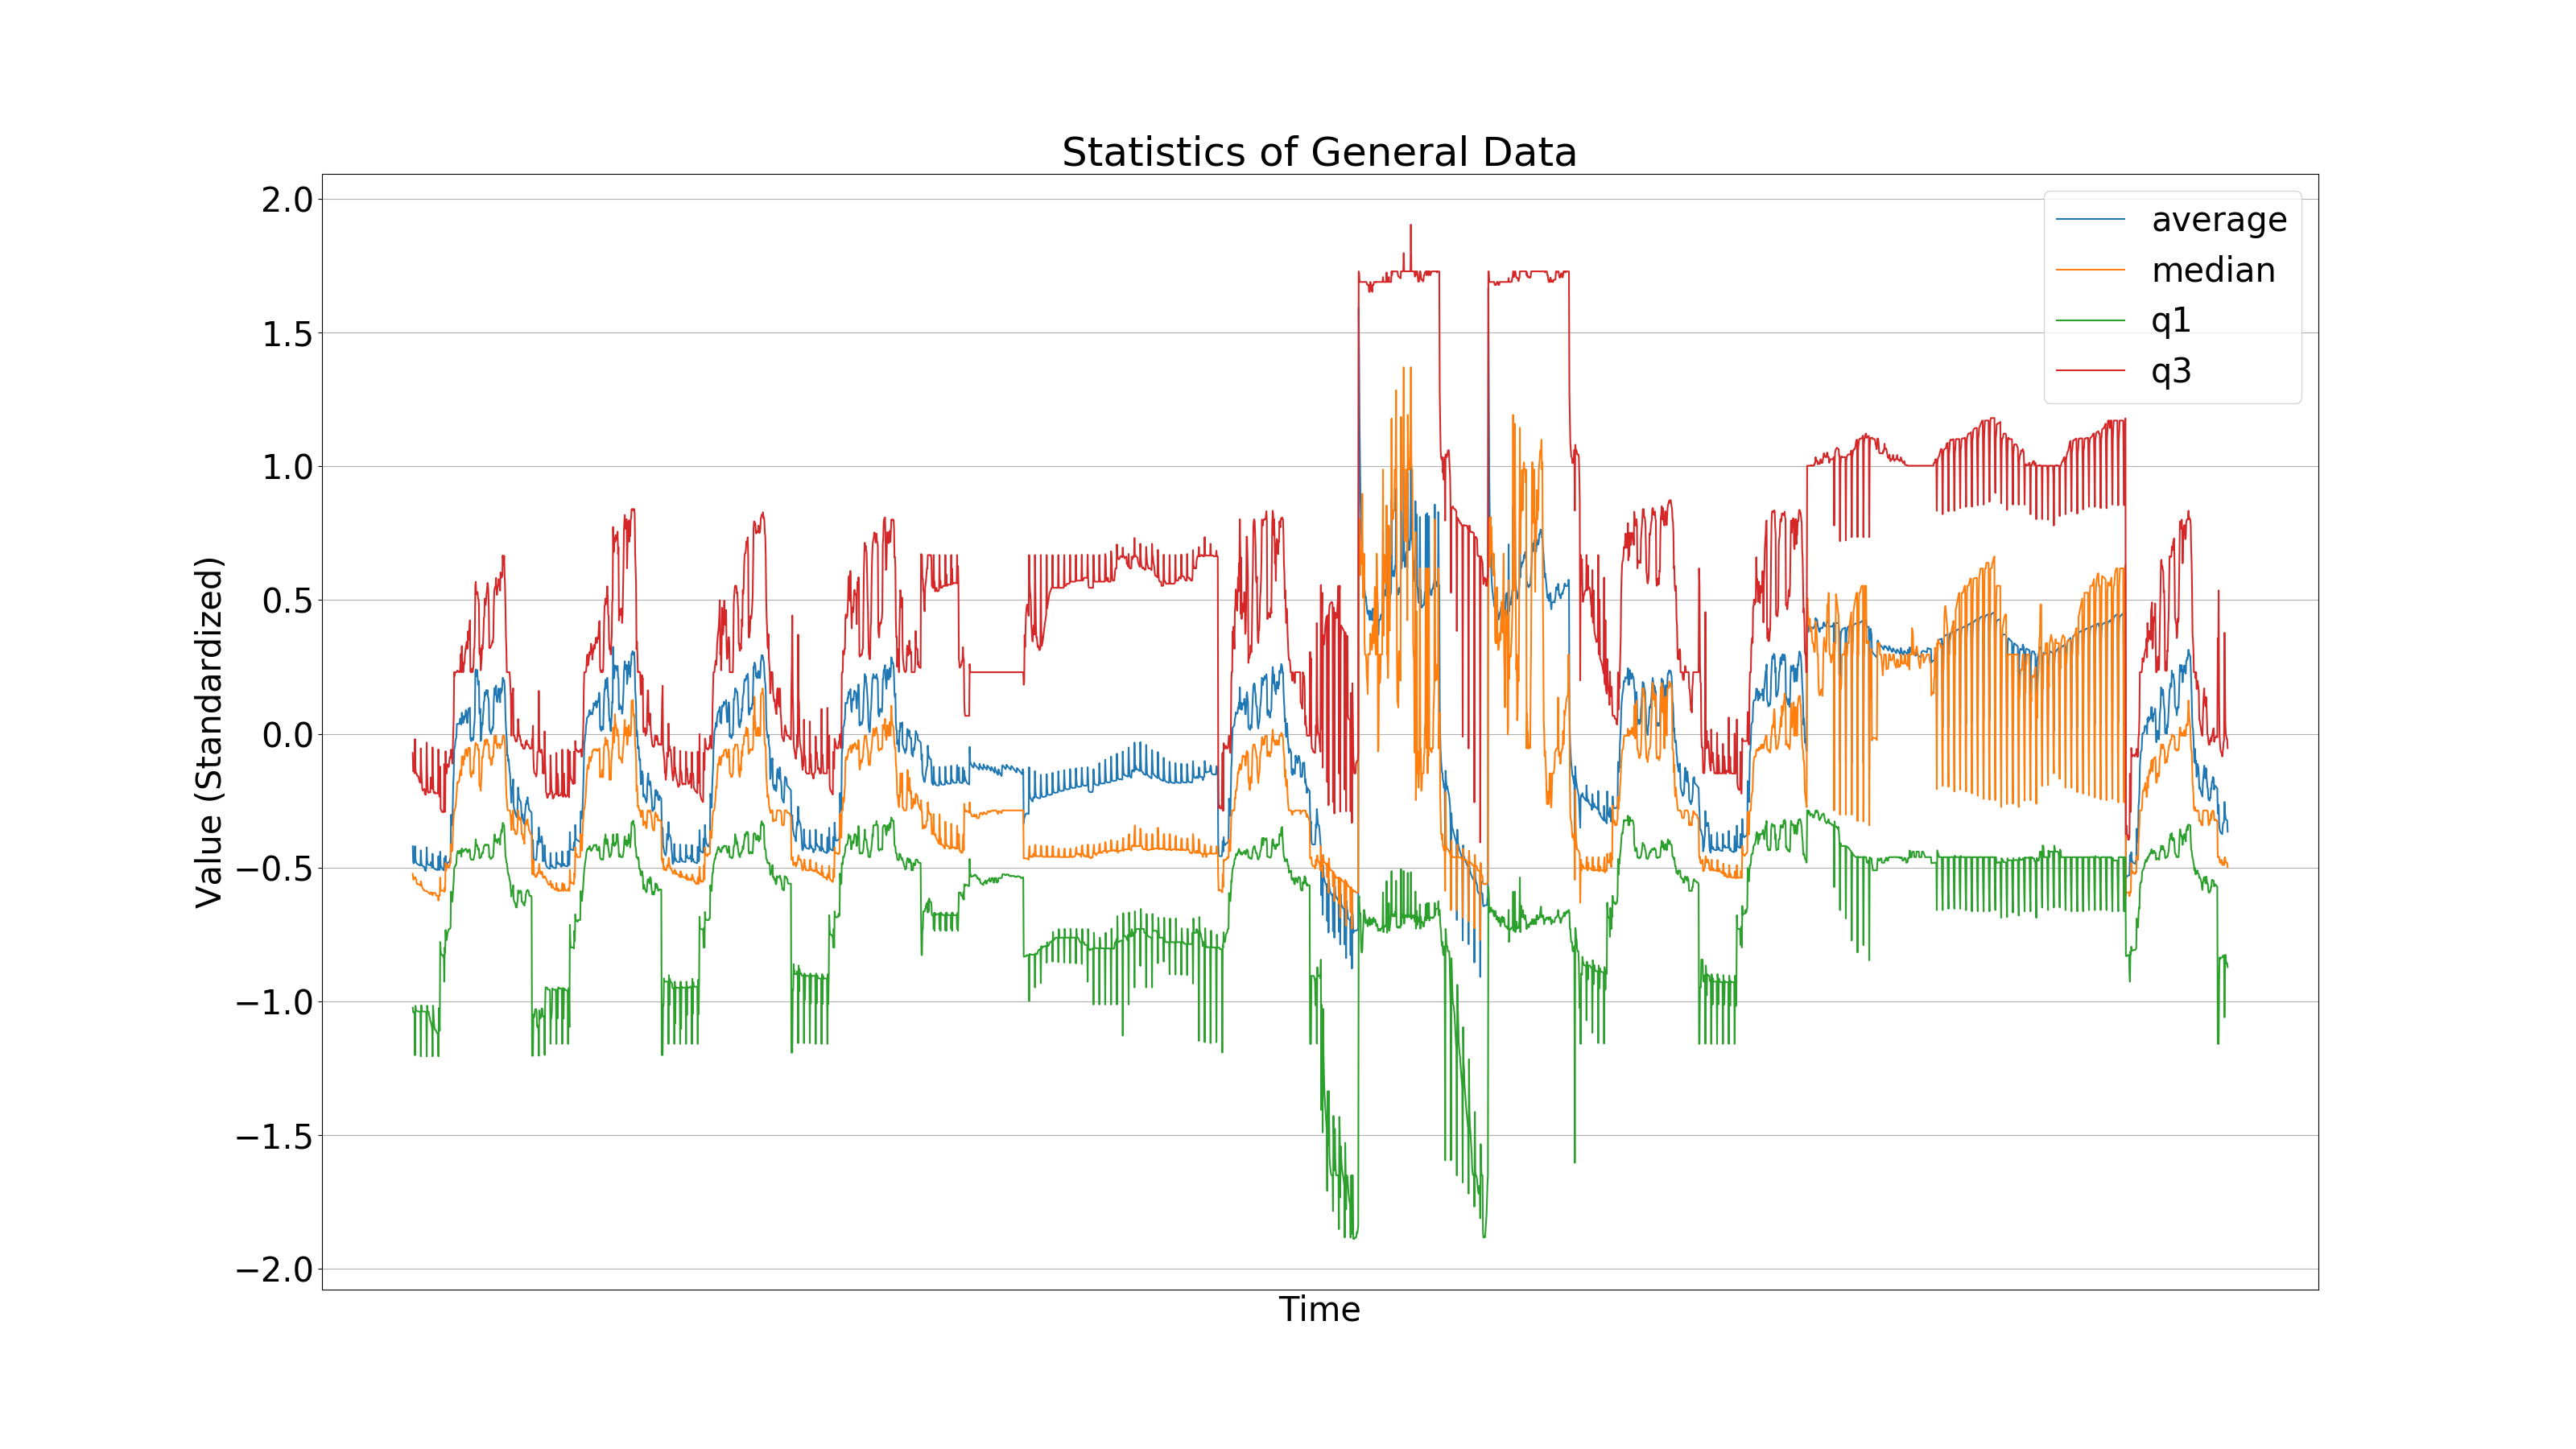
\includegraphics[width=0.4 \linewidth]{figures/general2.png}
                        \\
                        
                        \mbox{(a) Stacked} & \mbox{(b) Statistics} \\
                    \end{array}$
                    \caption{Plots of General Building Data}
                    \label{fig:general}
                \end{figure}
            
                In the first-quarter, we find that the general building data make a cycle every \textit{288 indices} as figure \ref{fig:firstq}. The general building data are reported on every 5 minutes, so the general building data make a cycle every \textit{1440 minutes} or every \textit{24 hours} or every \textit{1 day}. 
                
                \begin{figure}[htbp]
                    \centering
                    $\begin{array}{cc}
                        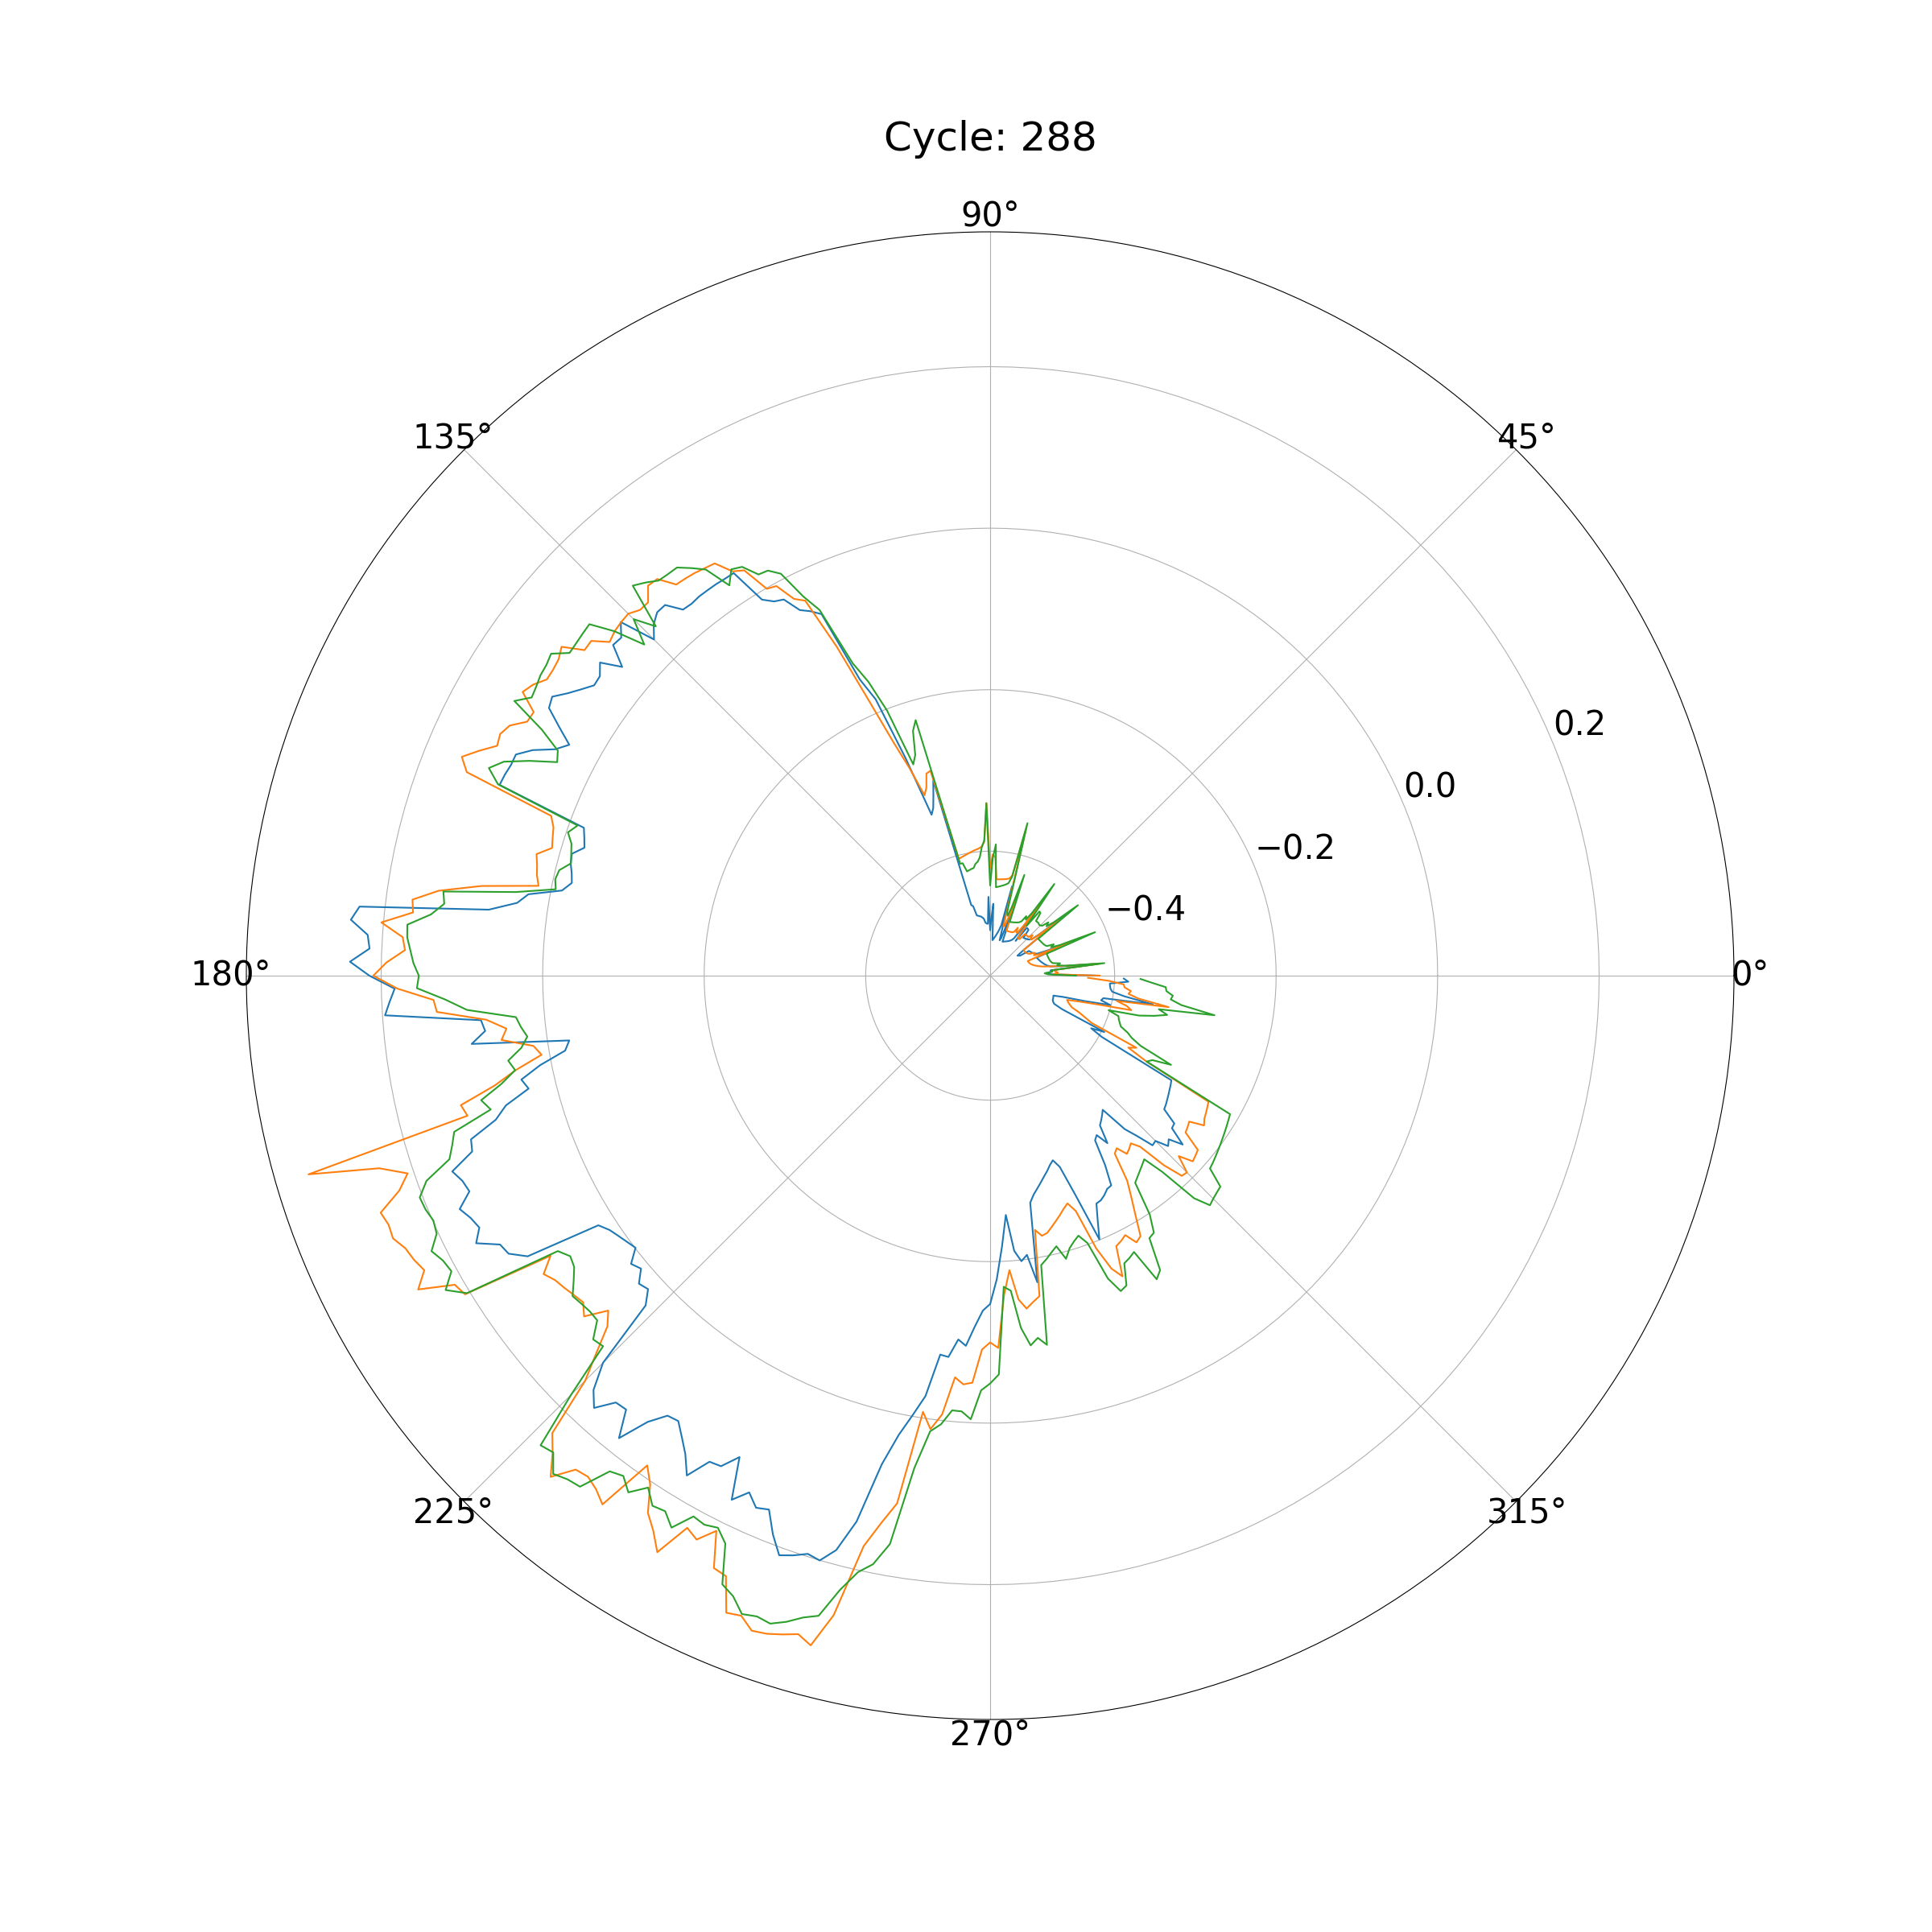
\includegraphics[width=0.3 \linewidth]{figures/polar1.png}
                        &
                        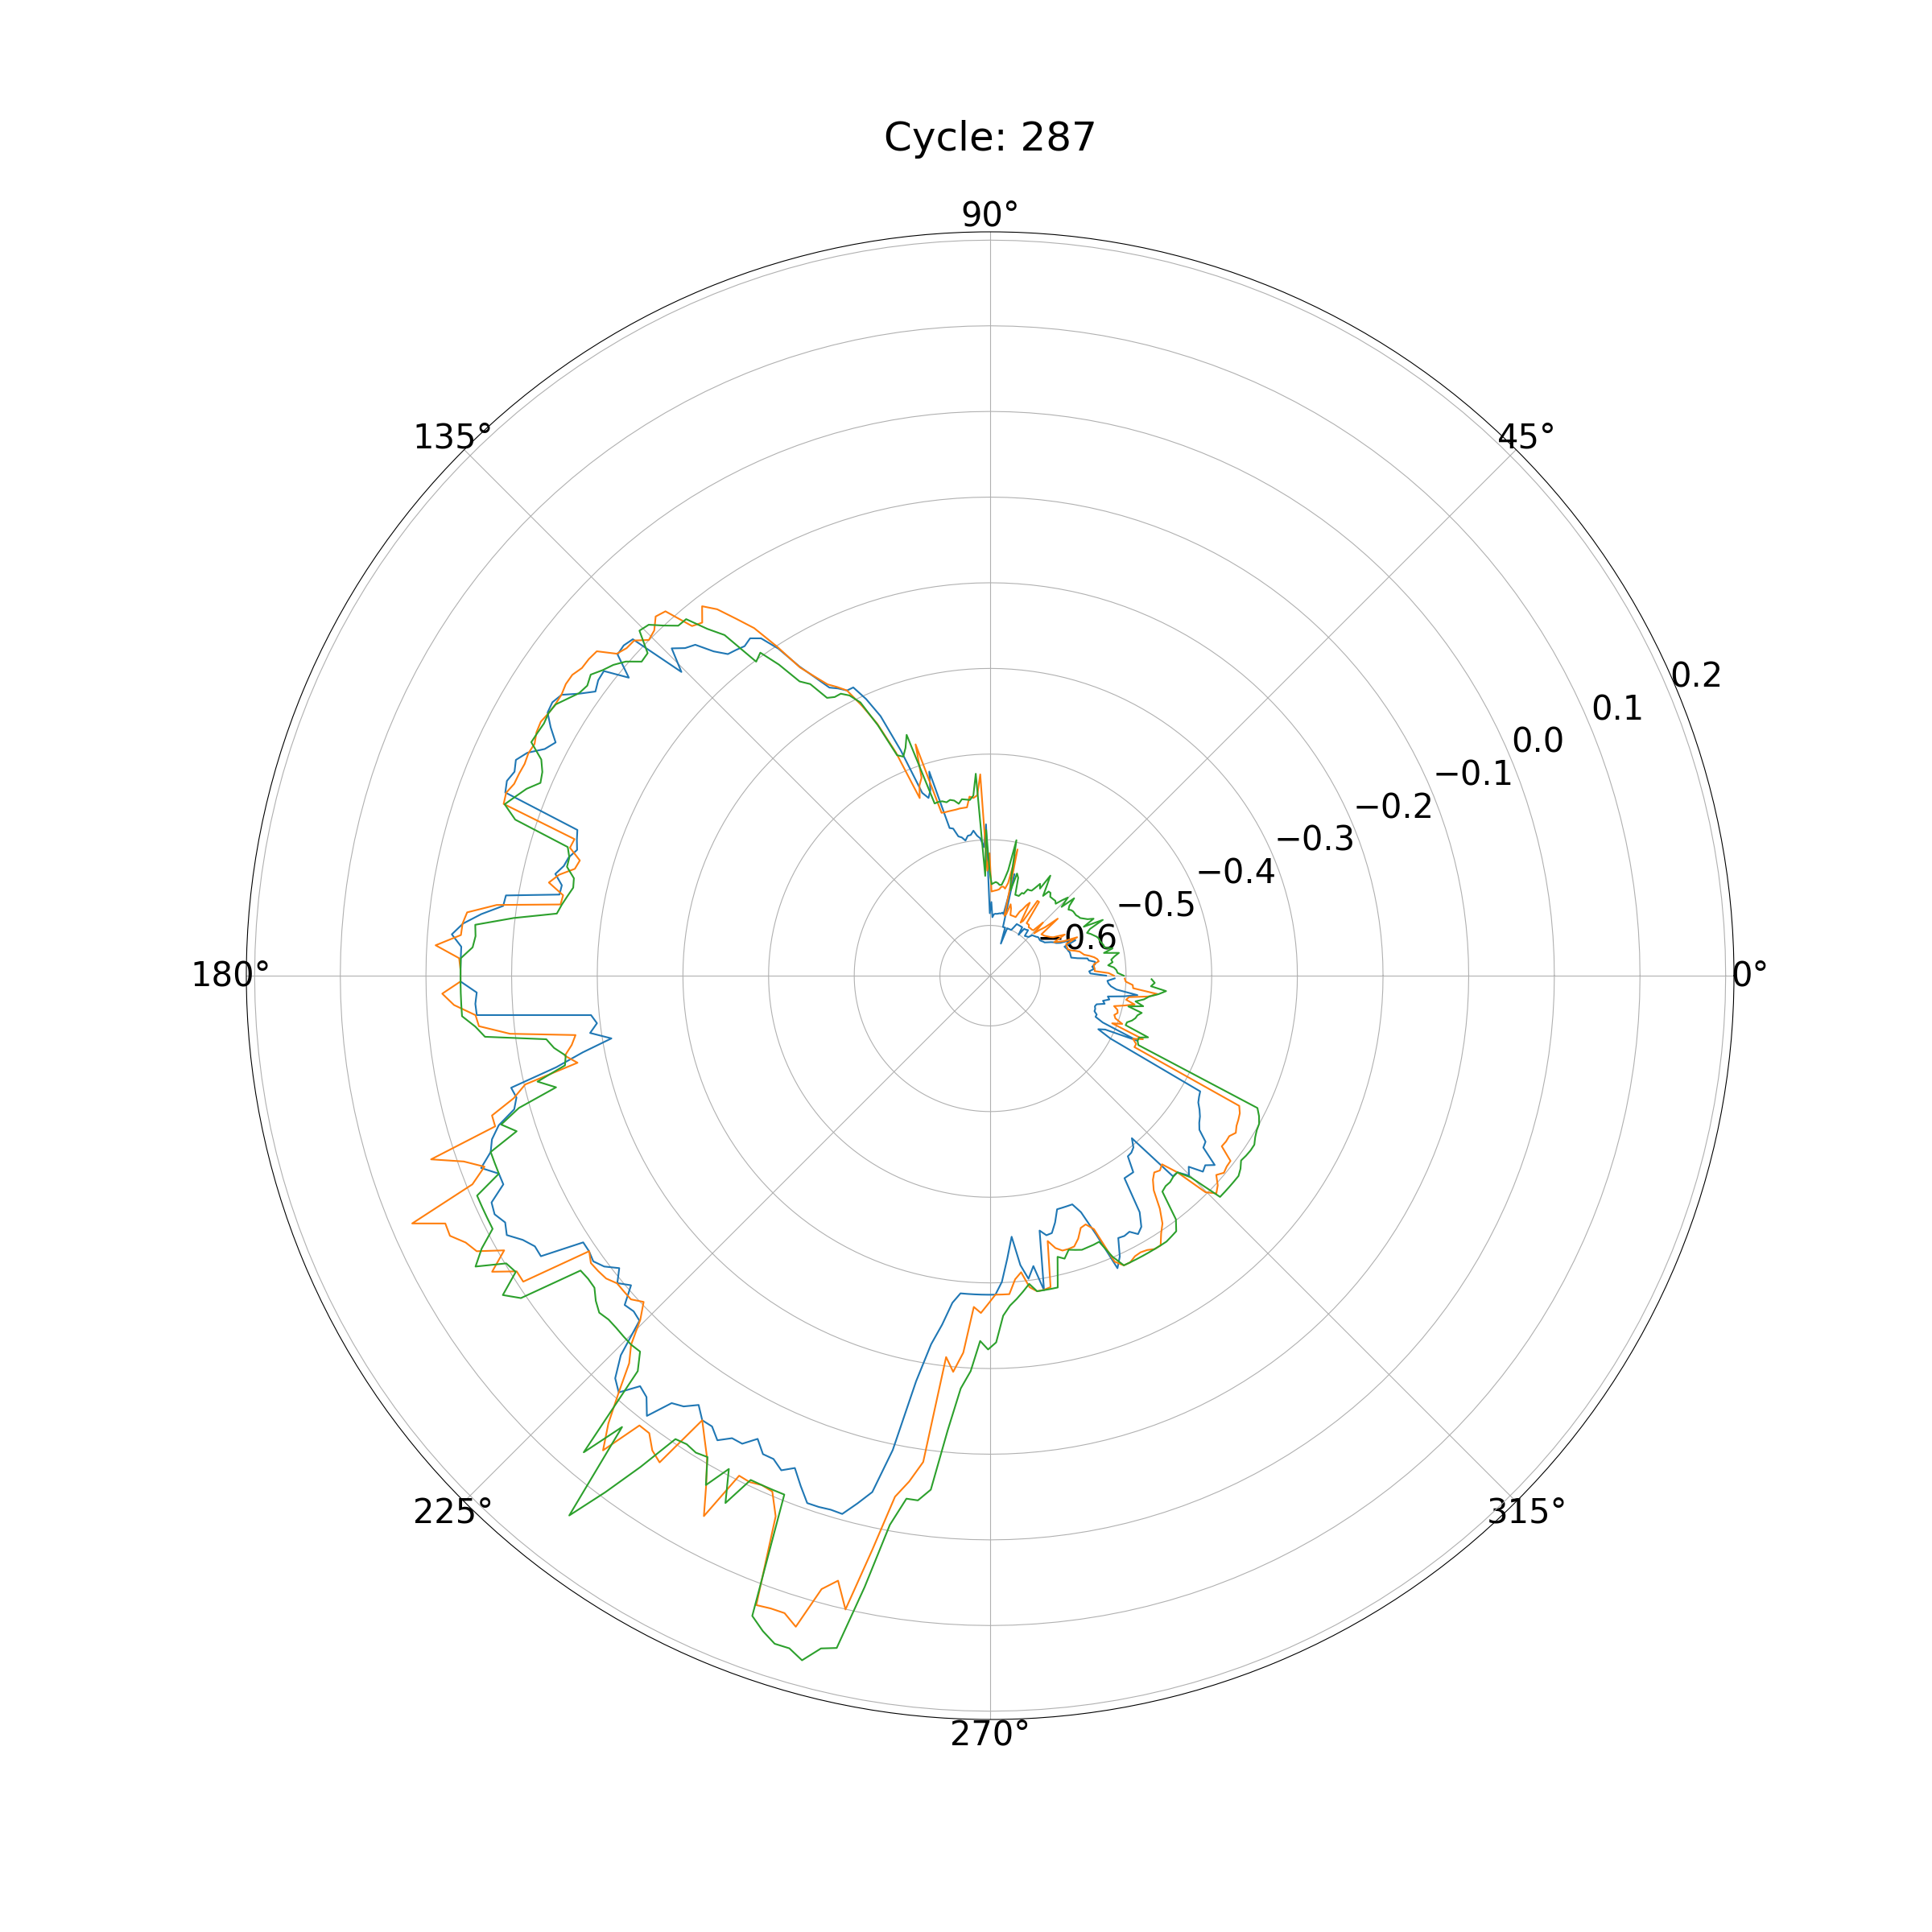
\includegraphics[width=0.3 \linewidth]{figures/polar2.png}
                        \\
                        \mbox{(a) Mean} & \mbox{(b) Median} \\
                        
                        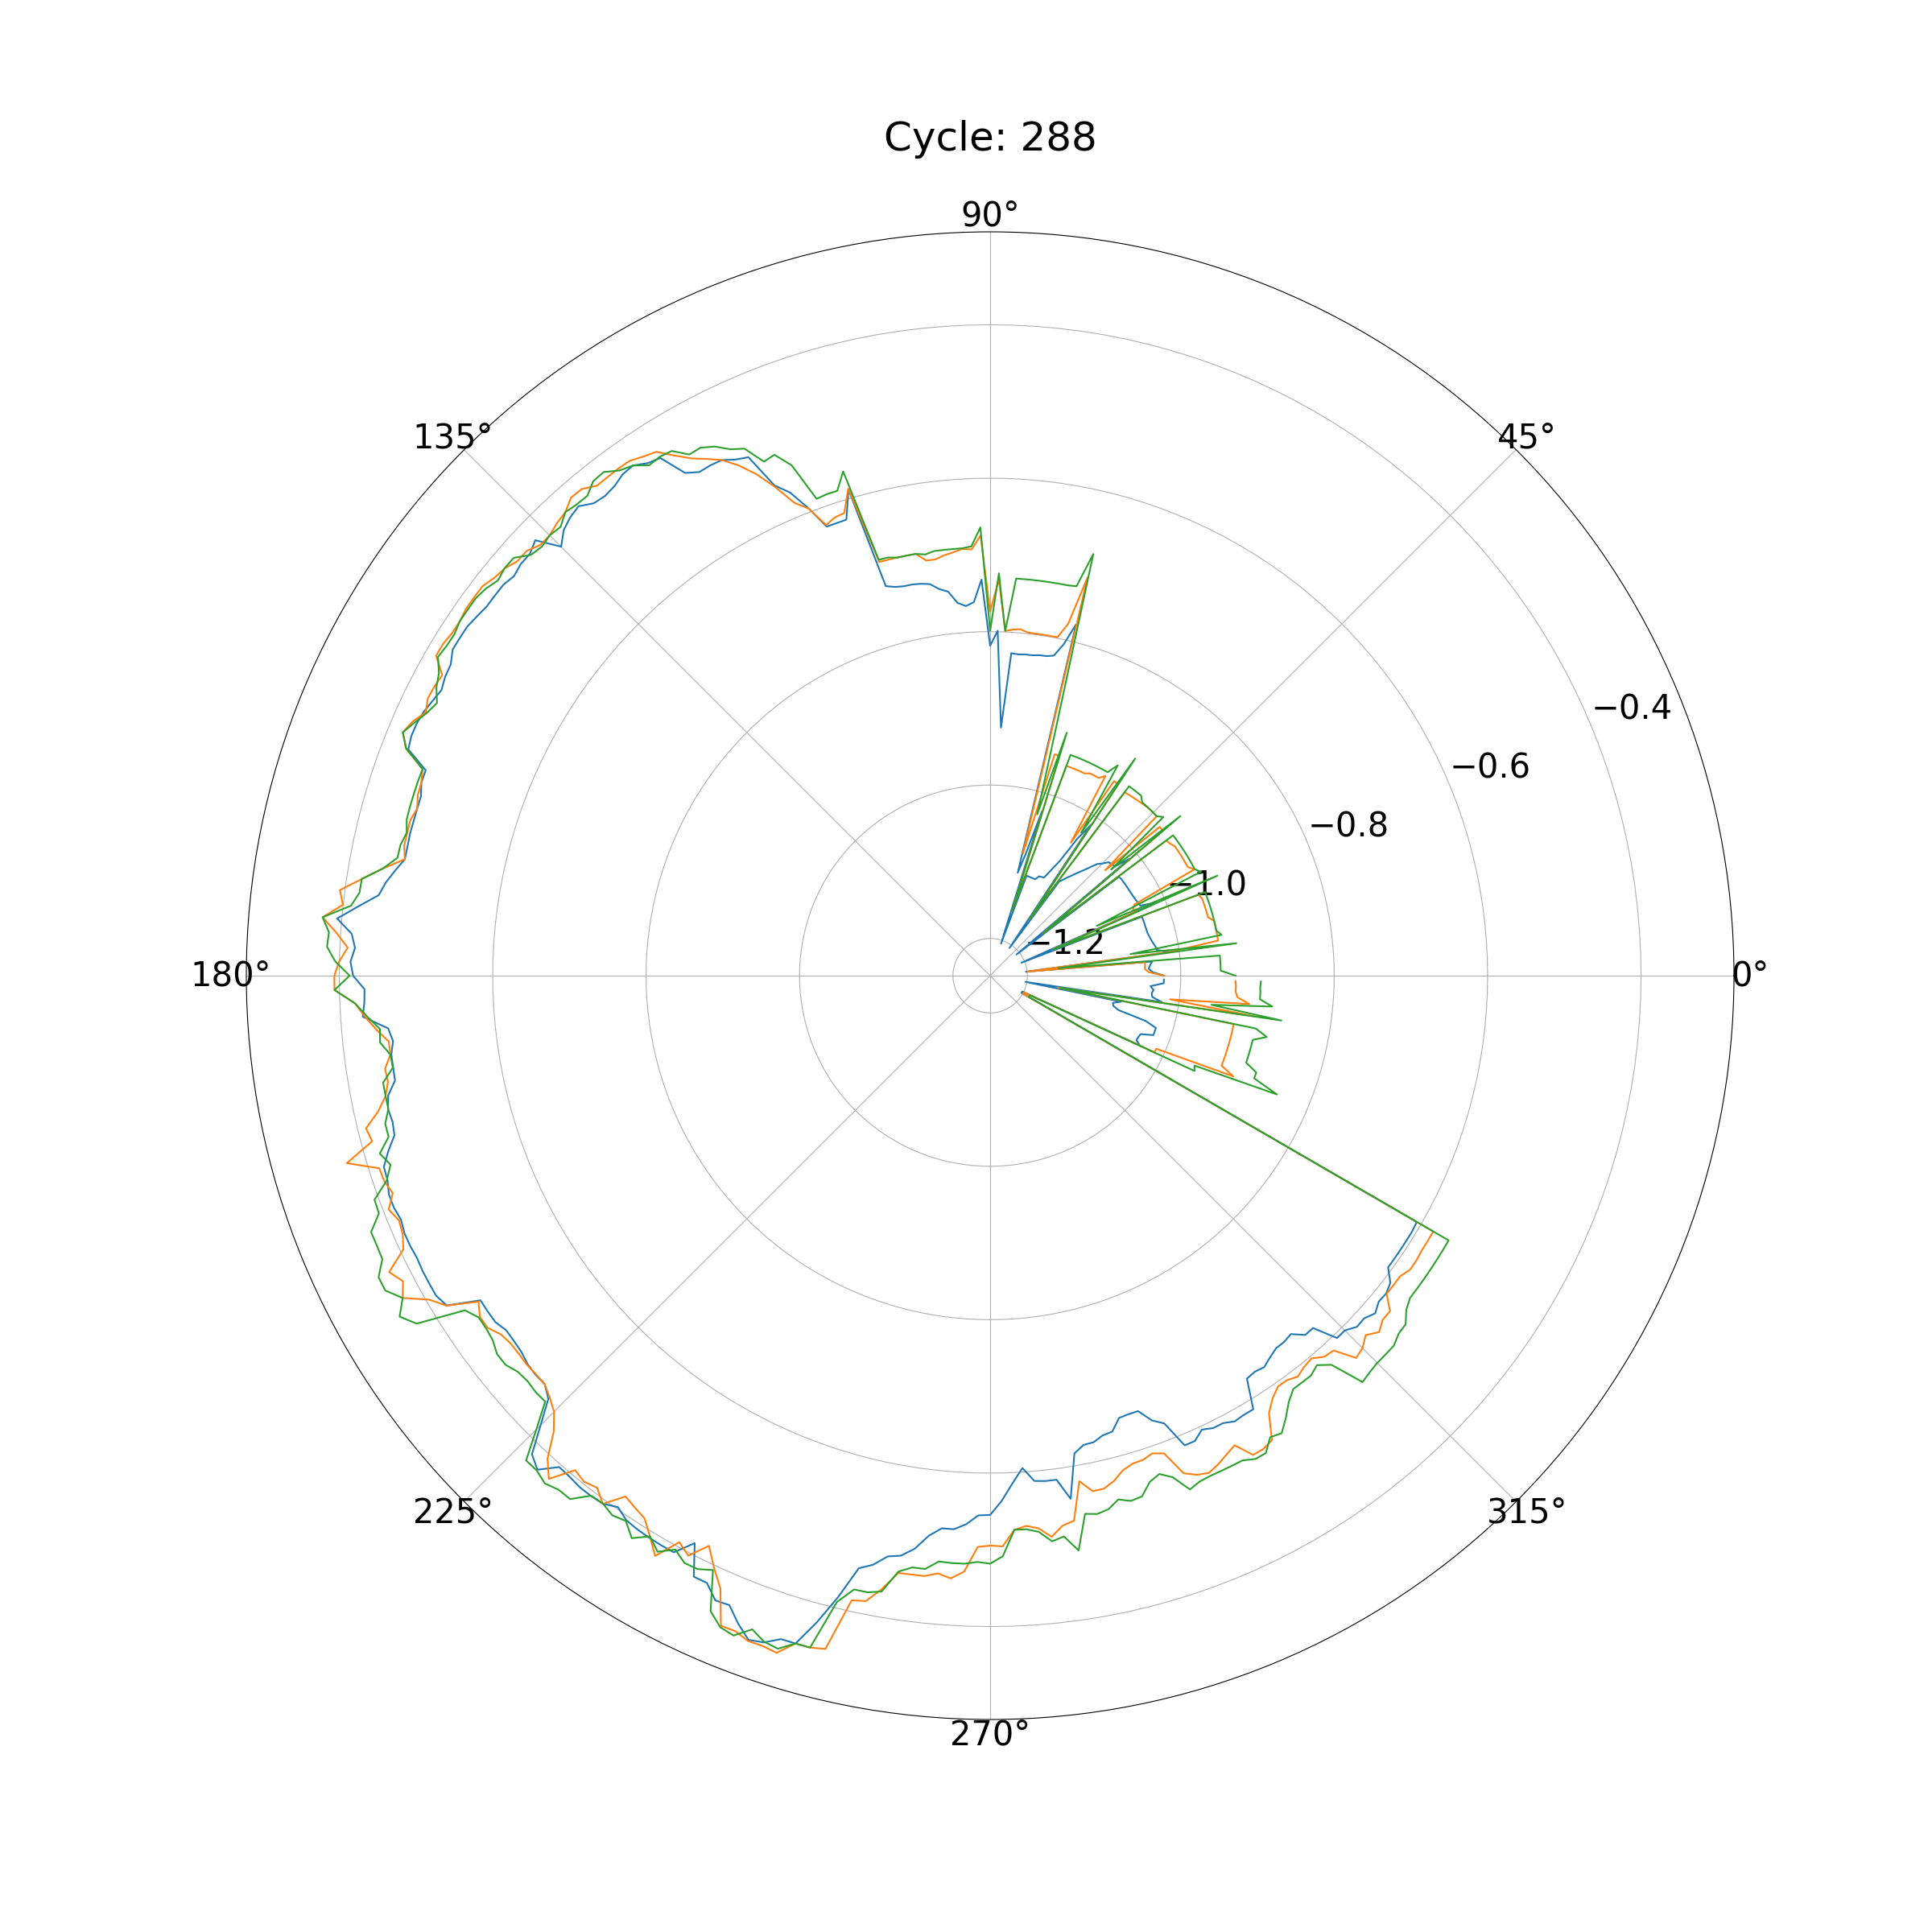
\includegraphics[width=0.3 \linewidth]{figures/polar3.png}
                        &
                        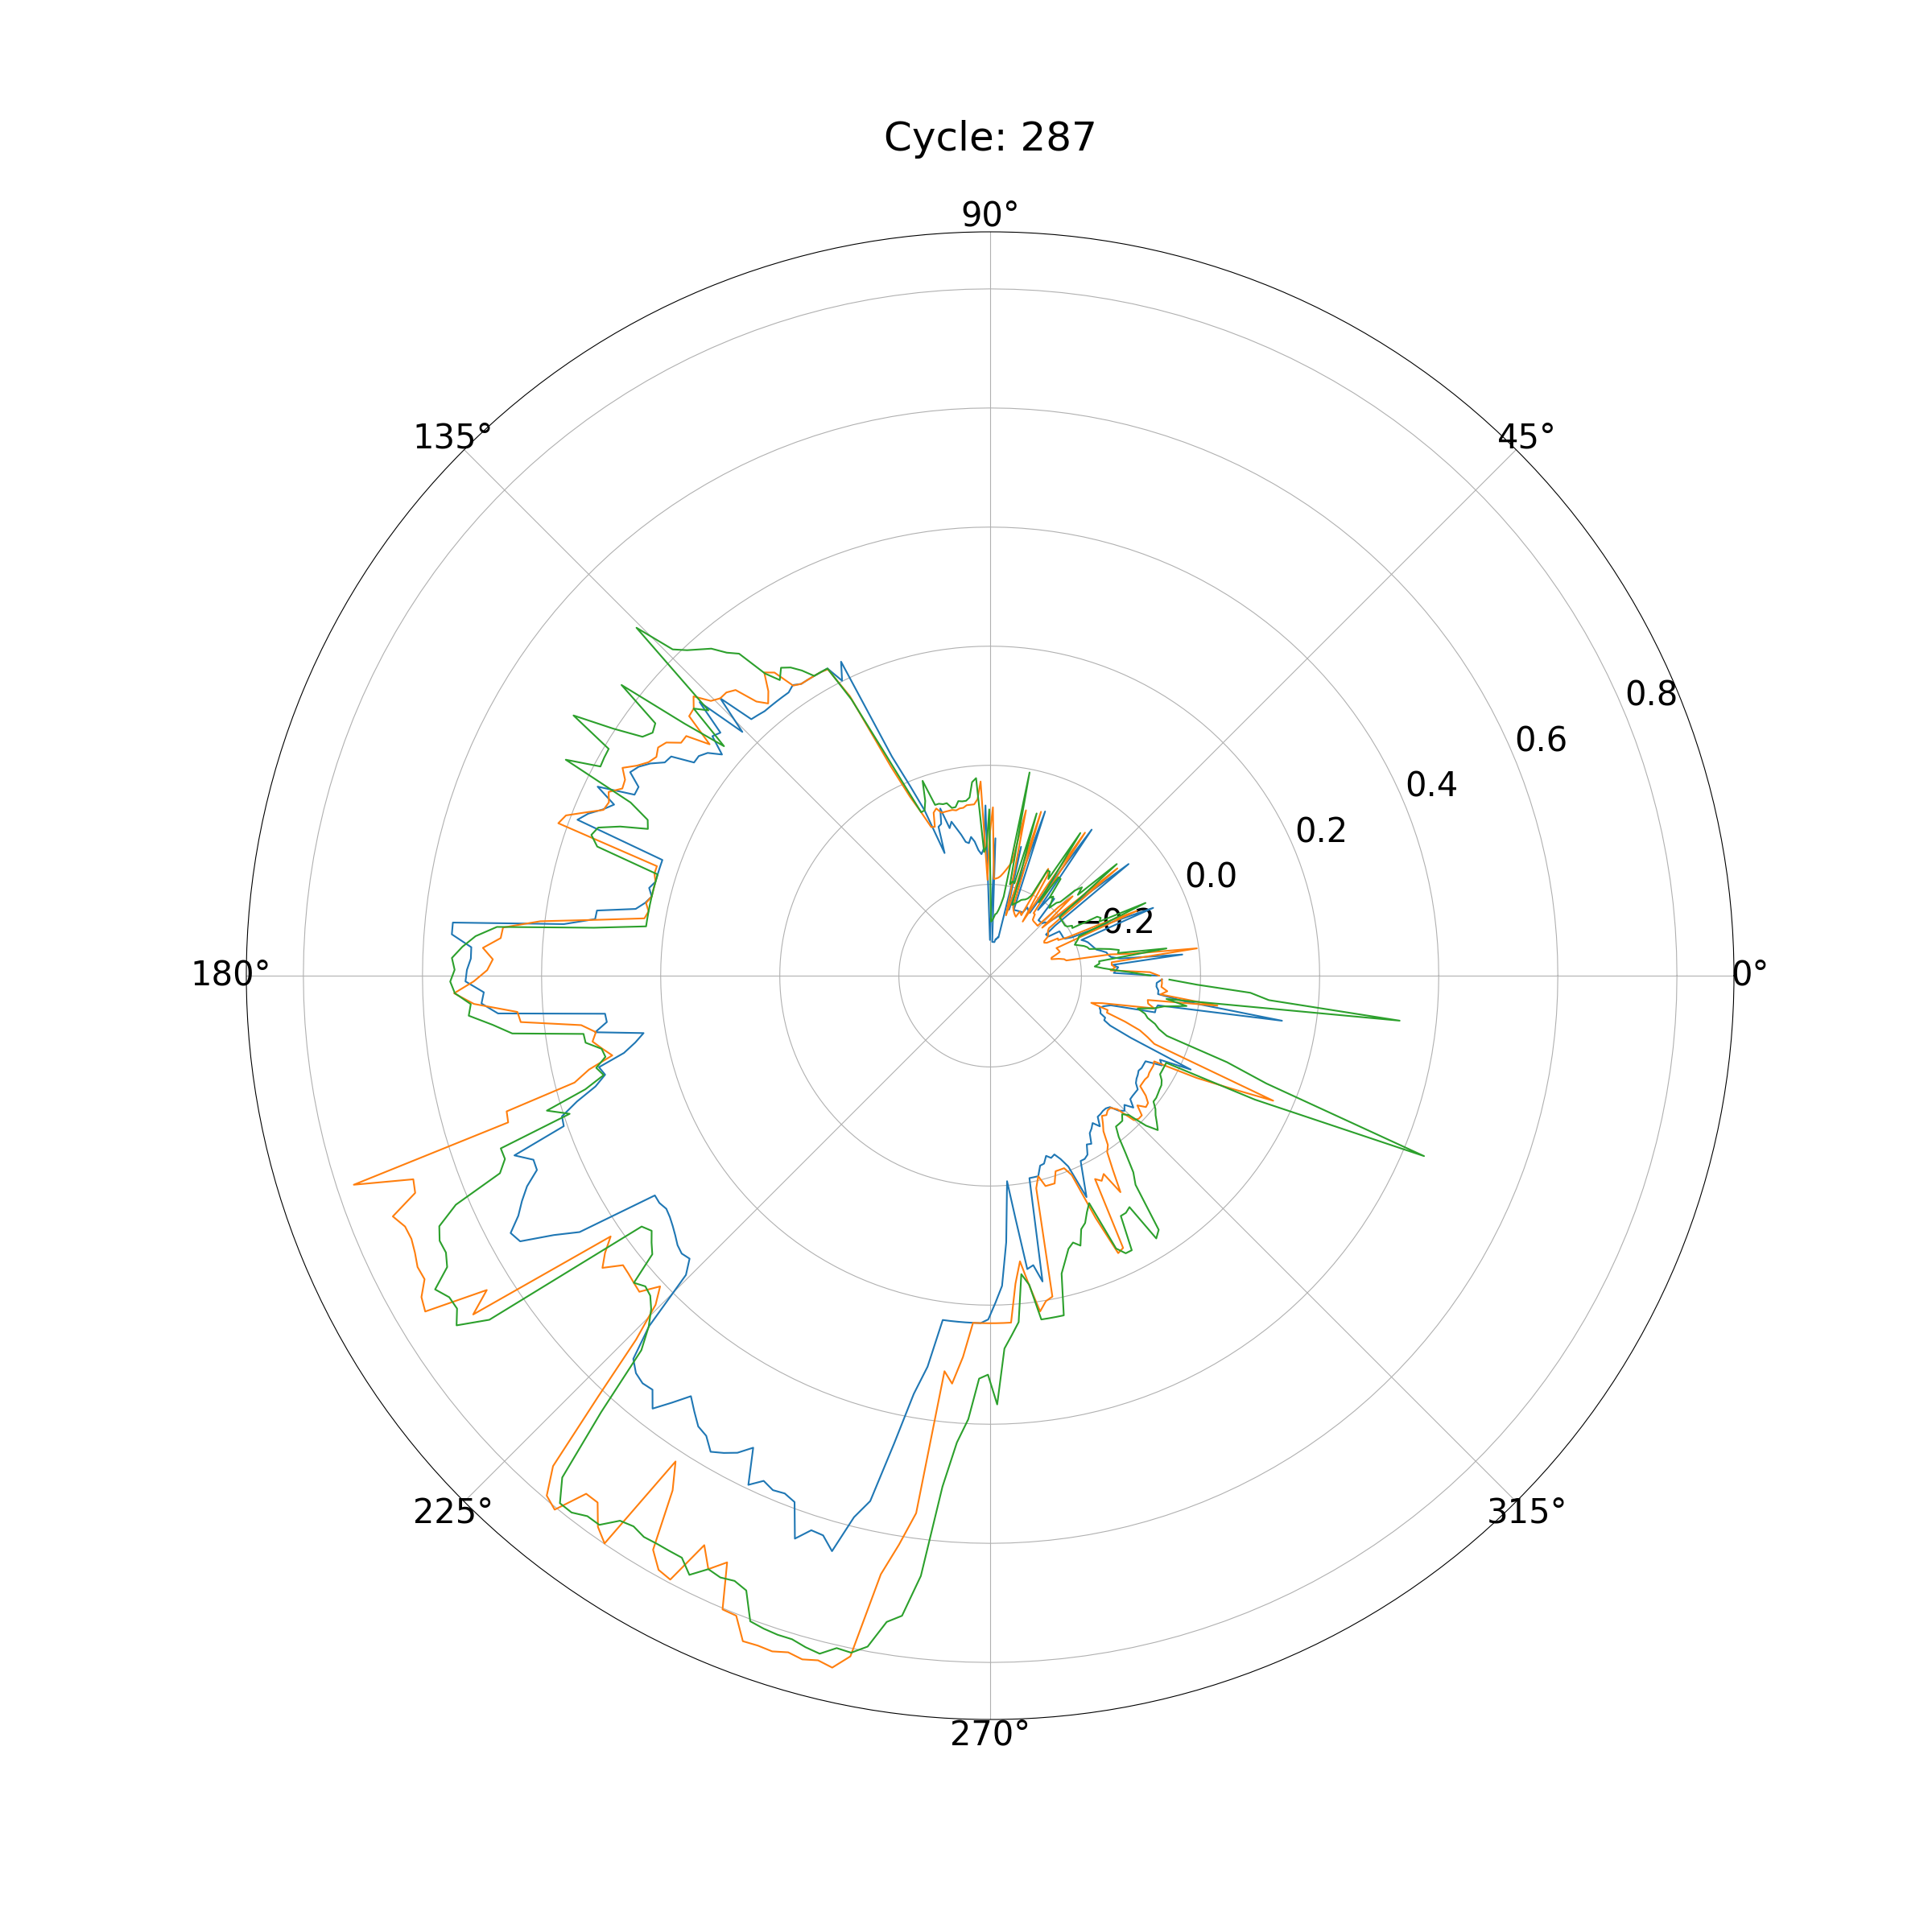
\includegraphics[width=0.3 \linewidth]{figures/polar4.png}
                        \\
                        \mbox{(c) q1} & \mbox{(d) q3} \\
                    \end{array}$
                    \caption{Cyclic Plots on First-quarters}
                    \label{fig:firstq}
                \end{figure}
            
                In the second-quarter, we calculated the peak in every columns in general building data. With figure \ref{fig:secondq}-(a), the distribution of peak width is shown; and, with figure \ref{fig:secondq}-(b), you can know that where is peak in general building data. Also, table \ref{tb:secondq} displays basic statistics value of peak width. With the data in figure \ref{fig:secondq} and table \ref{tb:secondq}, we can know that the general building data are suddenly increasing about \textit{15 indices}; in other words, the general building data has steeps every \textit{75 minutes}. 
                
                \begin{table}[htbp]
                    \centering
                    \caption{Basic Statistics Data with the peak in the Second-quarter}
                    \label{tb:secondq}
                    \begin{tabular}{c||c|c|c|c|c|c|c}
                        Item & Minimum & Maximum & Mean & q1 & Median & q3 & Standard Deviation \\ \hline
                        Value & 1.0 & 808.45 & 15.98 & 1.51 & 3.71 & 12.0 & 55.36 \\
                    \end{tabular}
                \end{table}
            
                \begin{figure}[htbp]
                    \centering
                    $\begin{array}{cc}
                        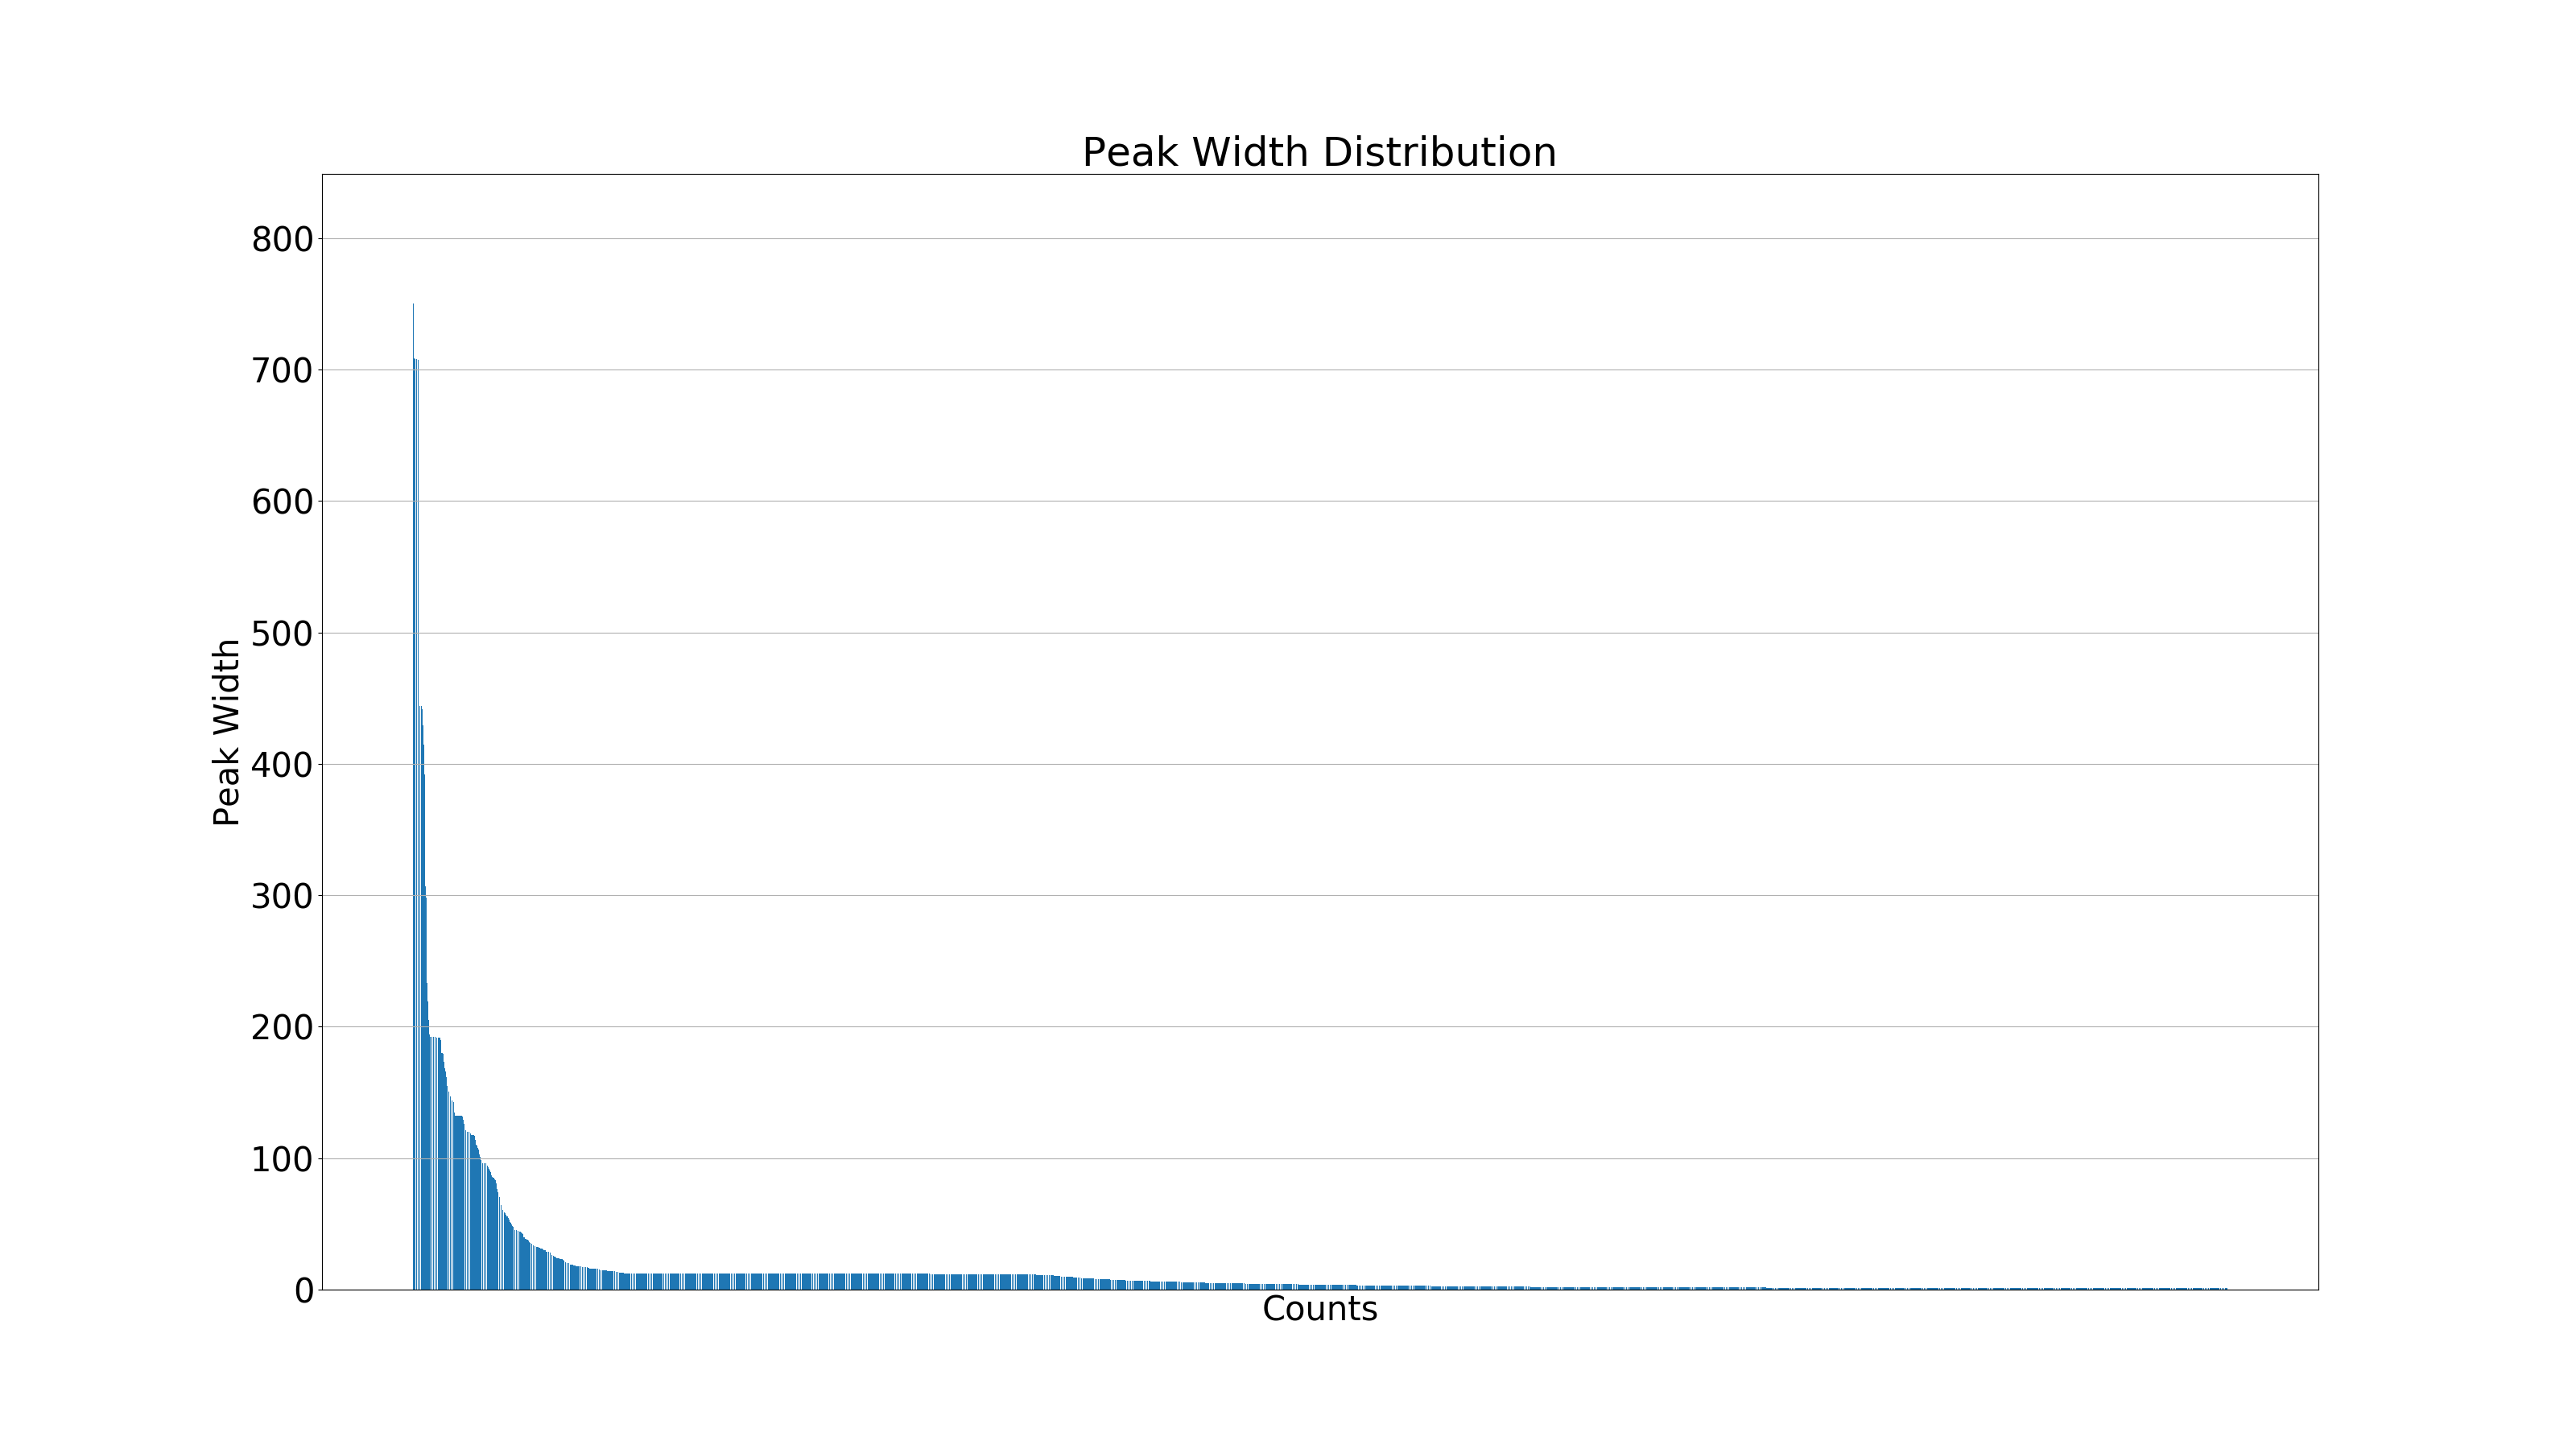
\includegraphics[width=0.4 \linewidth]{figures/second1.png}
                        &
                        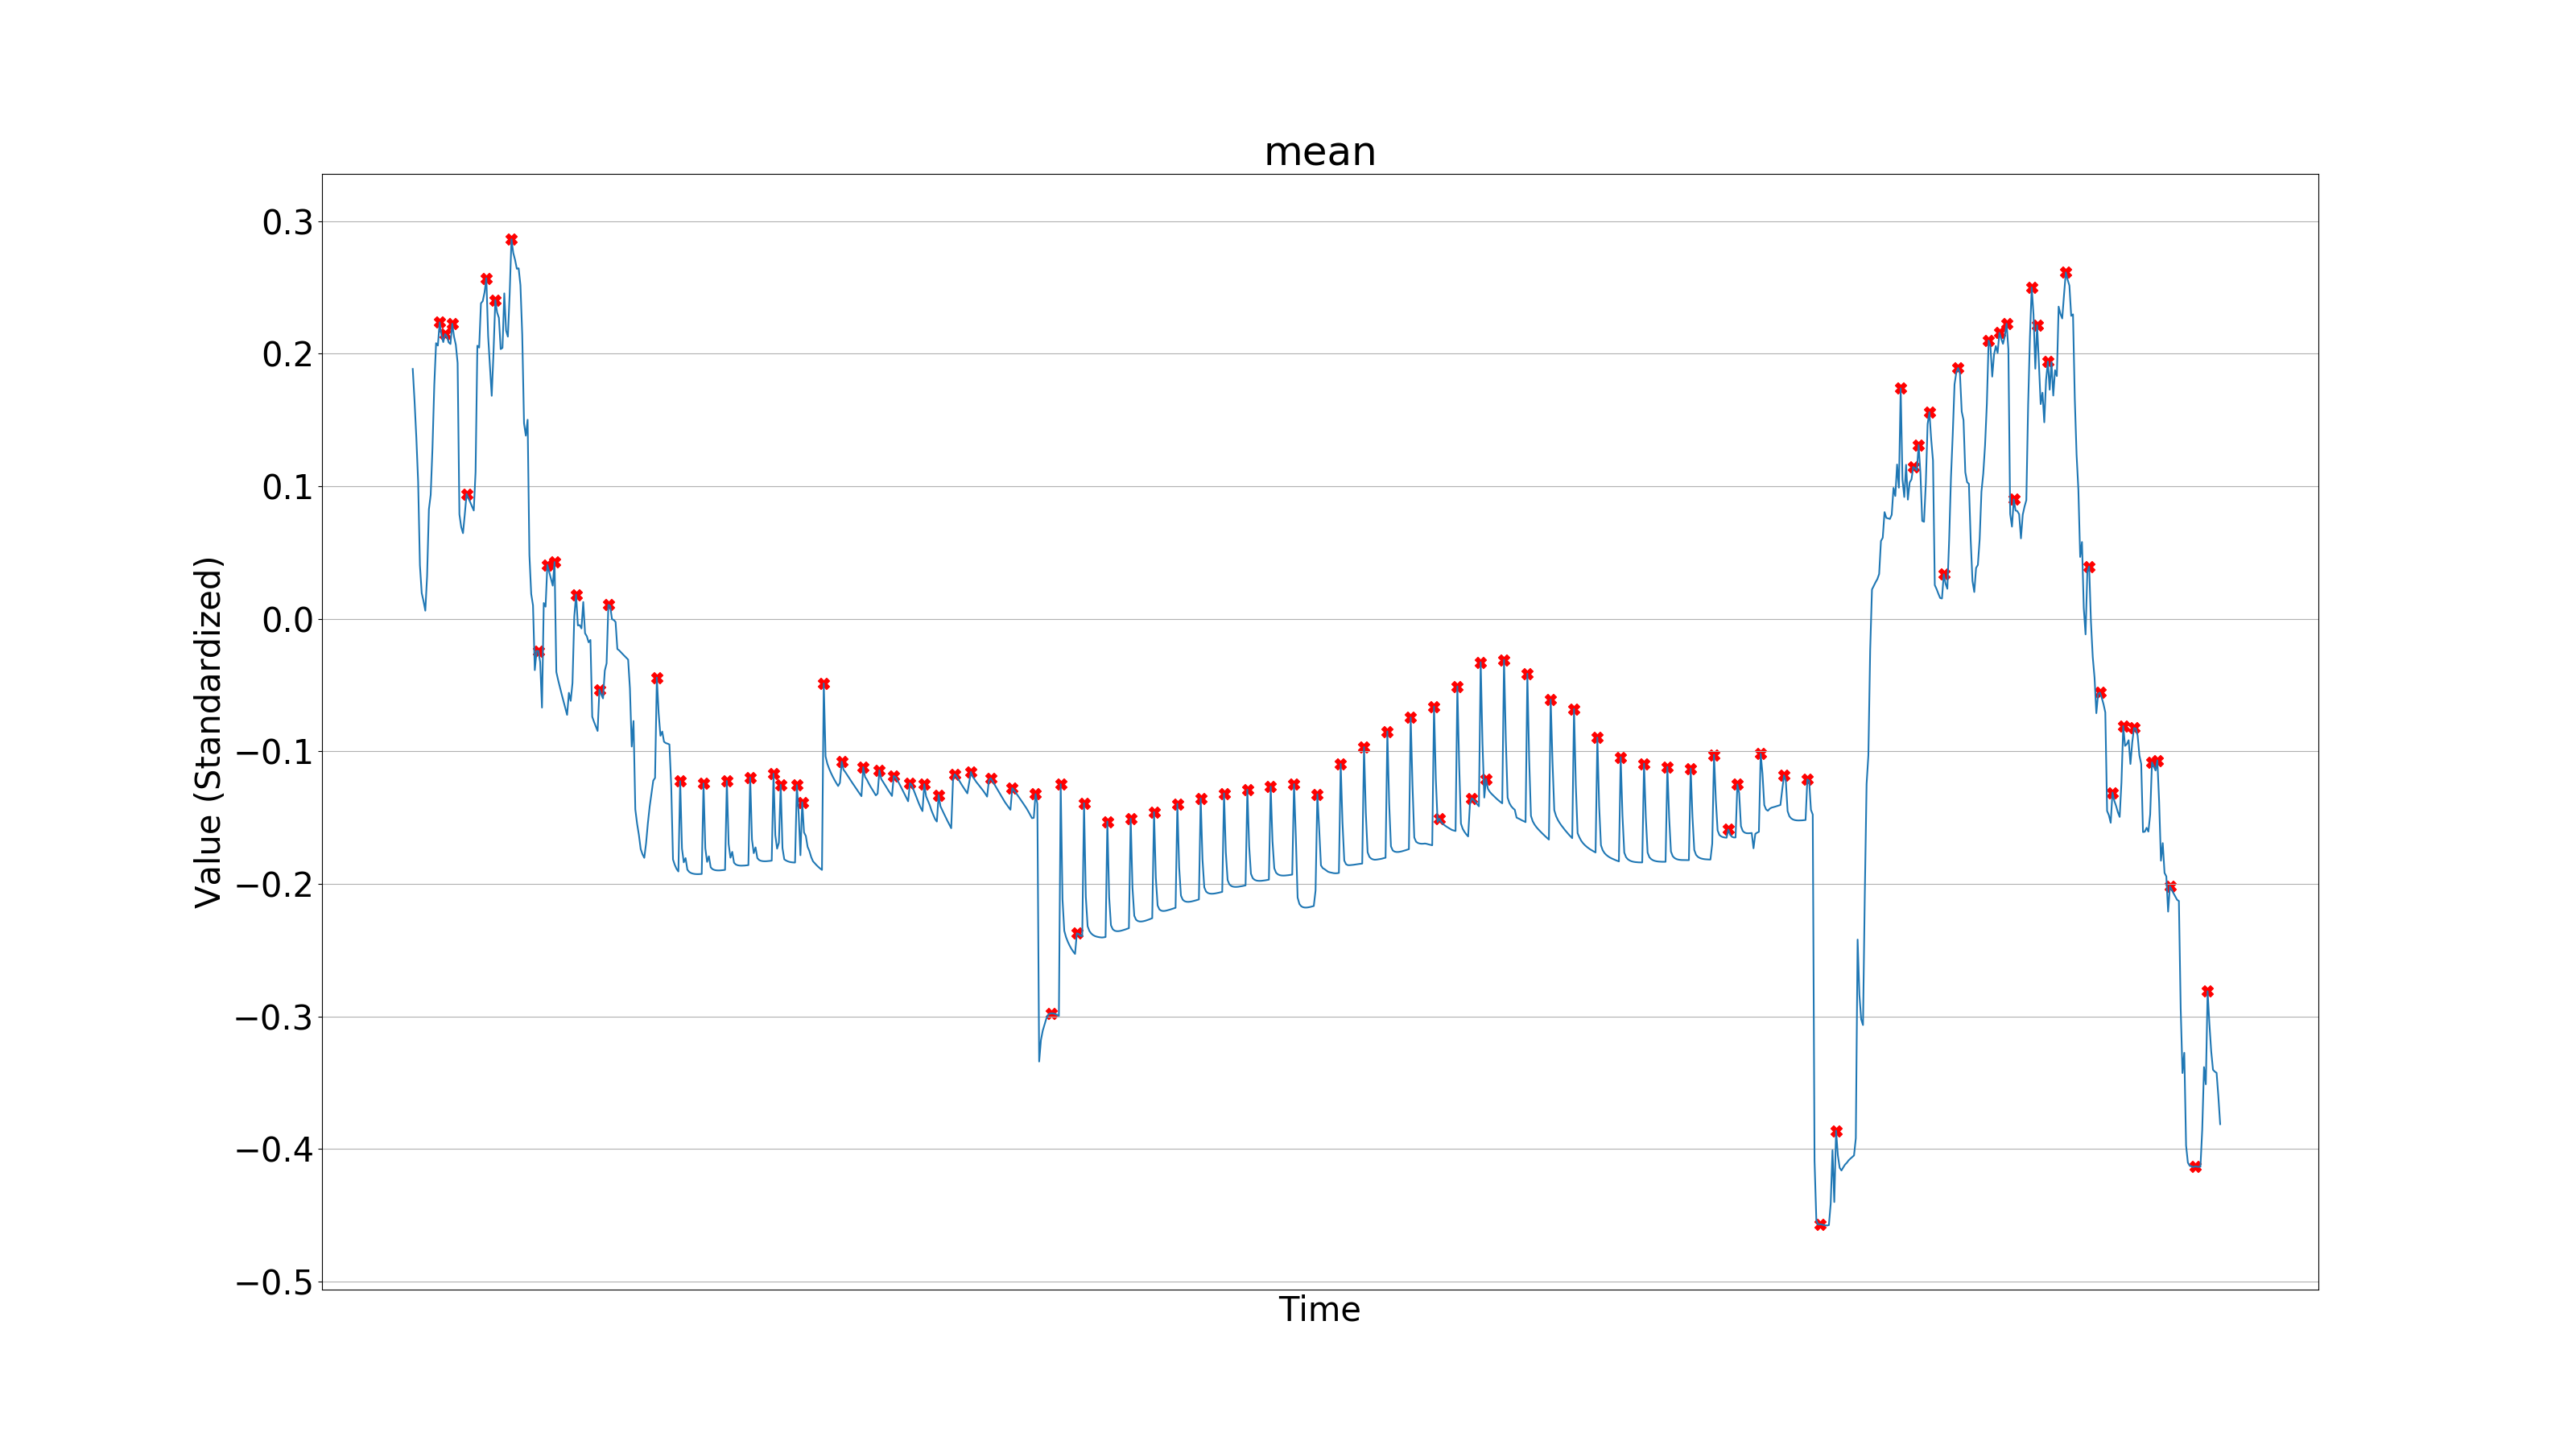
\includegraphics[width=0.4 \linewidth]{figures/second2.png}
                        \\
                        
                        \mbox{(a) Peak Width Distribution} & \mbox{(b) Peak in Mean Column}
                    \end{array}$
                    \caption{Peak in the Second-quarter}
                    \label{fig:secondq}
                \end{figure}
            
                As figure \ref{fig:firstq}, we drew the cyclic plots of the third-quarters of general building data as figure \ref{fig:thirdq}. As the first-quarters, the period is \textit{288 indices}, \textit{24 hours}, or \textit{1 day}. Therefore, there are two days which has increased general building data. 
            
                \begin{figure}[htbp]
                    \centering
                    $\begin{array}{cc}
                    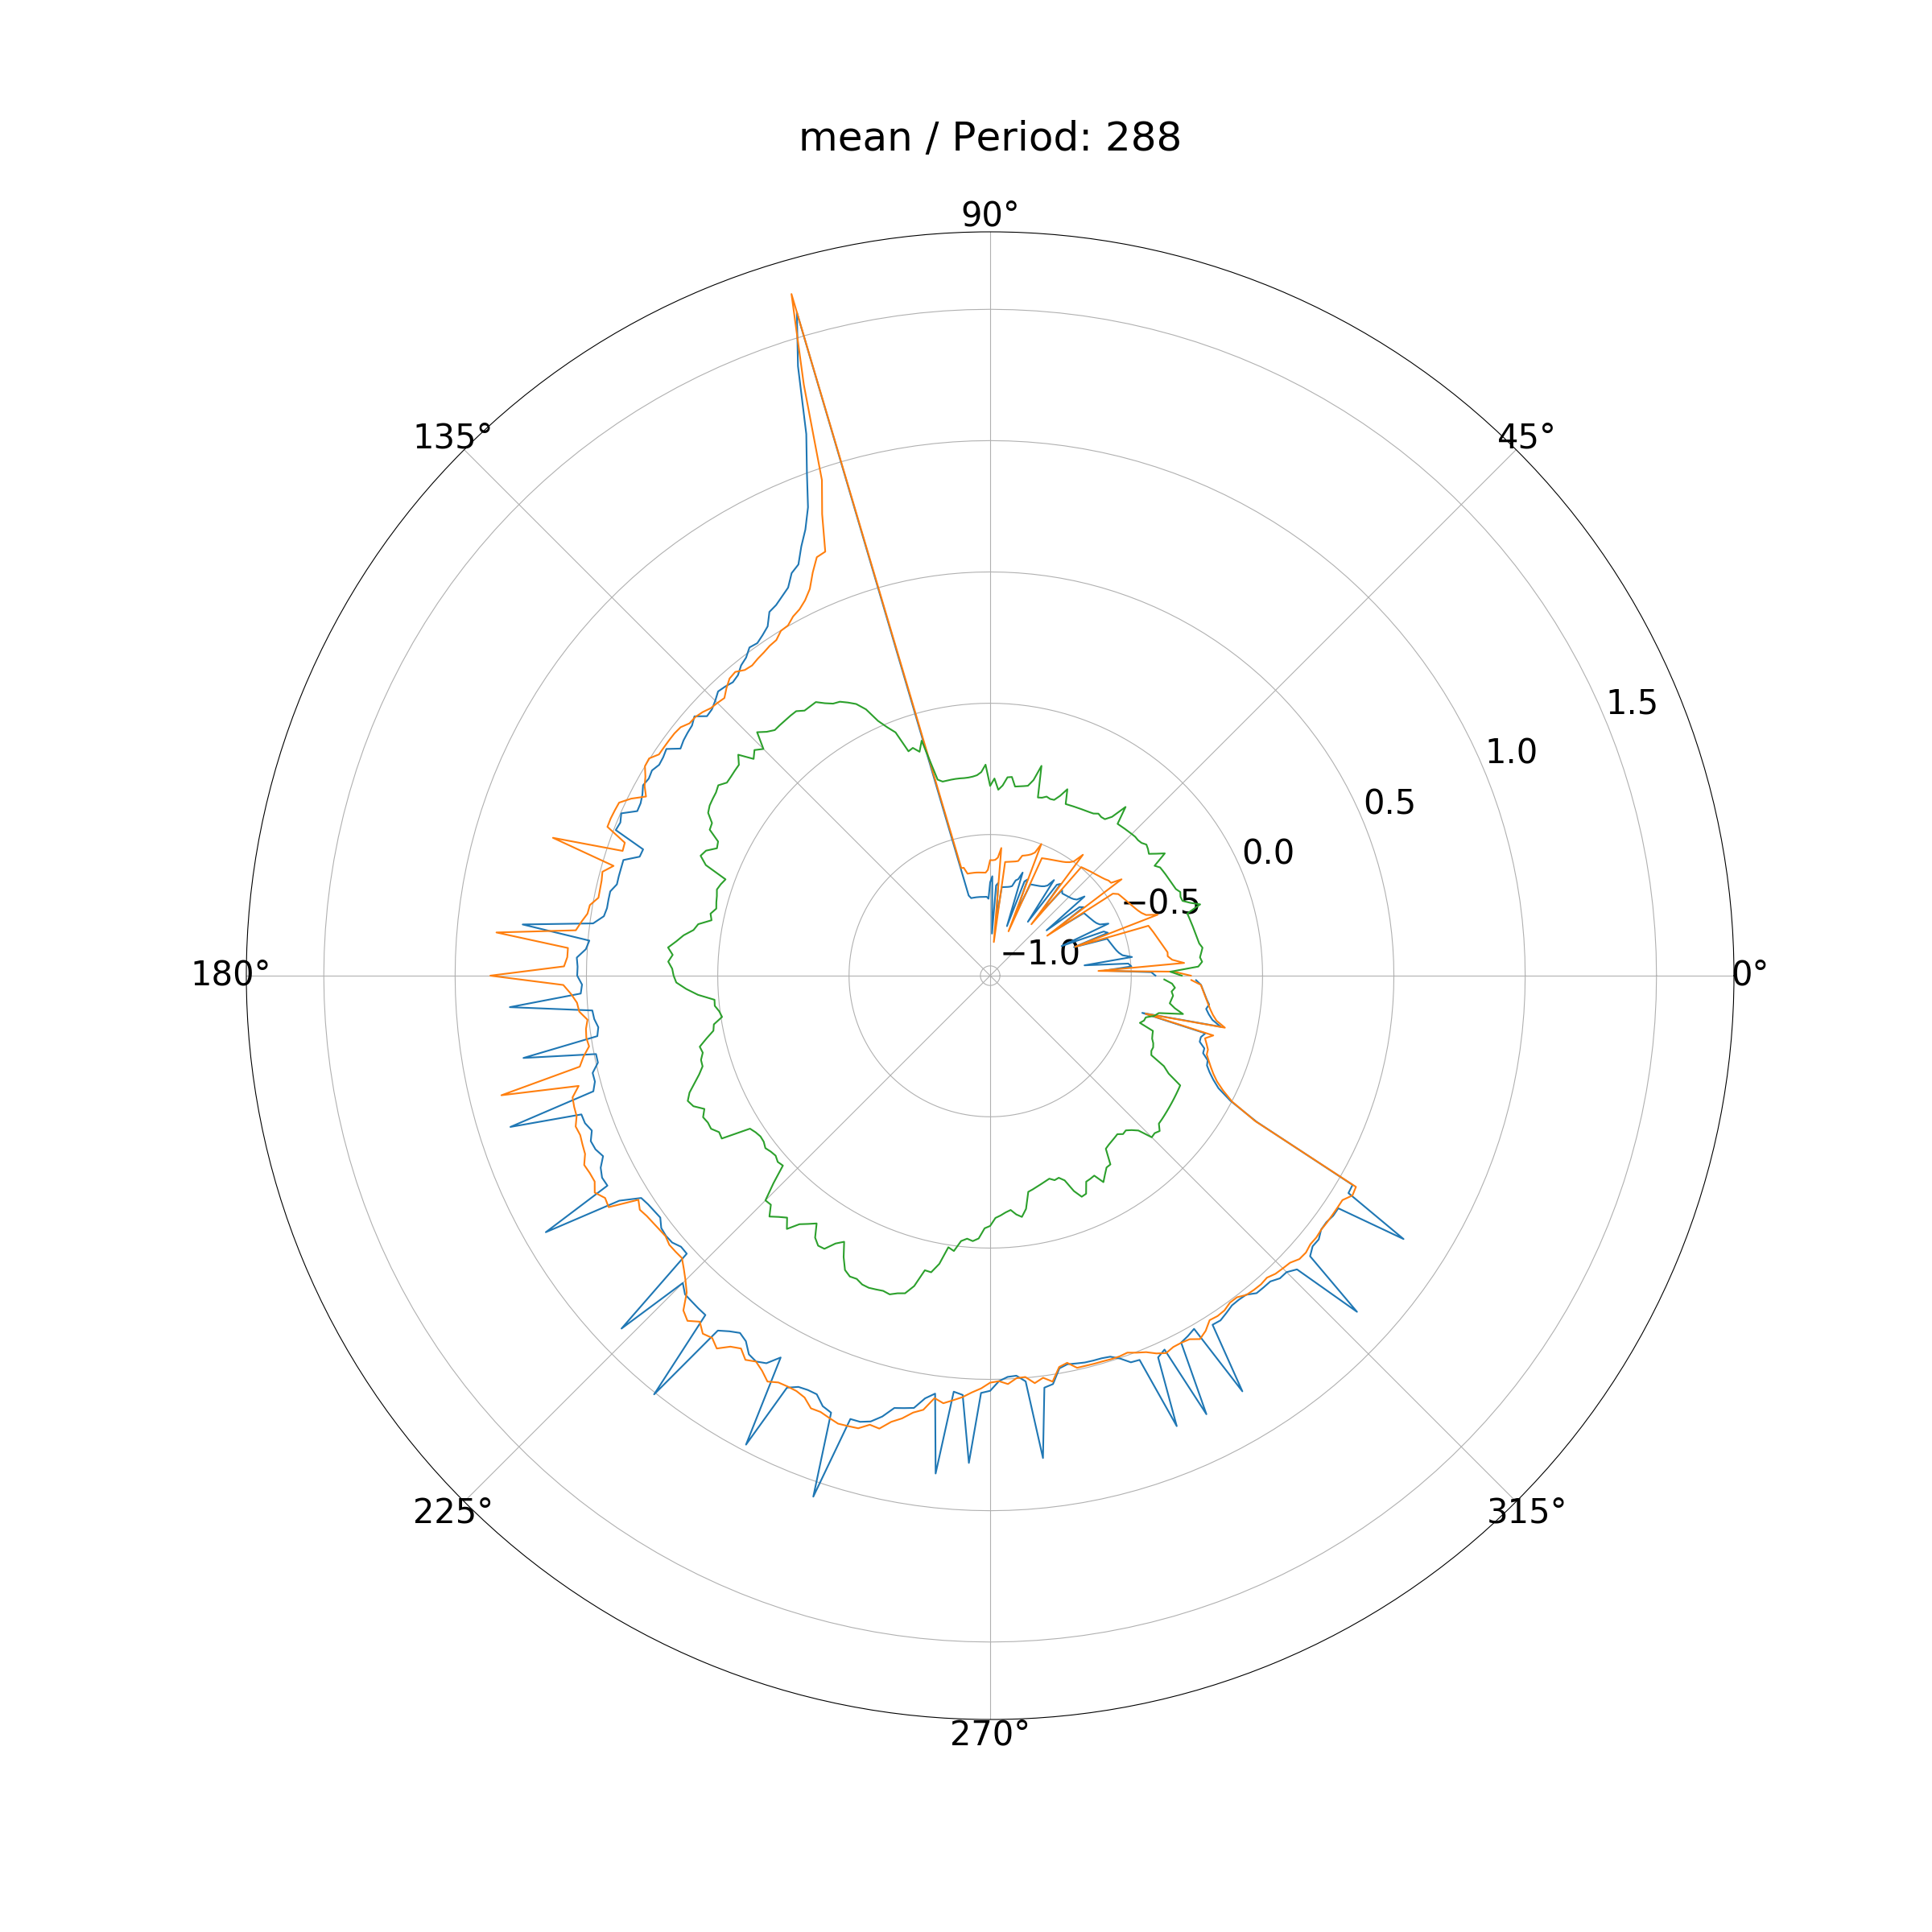
\includegraphics[width=0.3 \linewidth]{figures/third1.png}
                    &
                    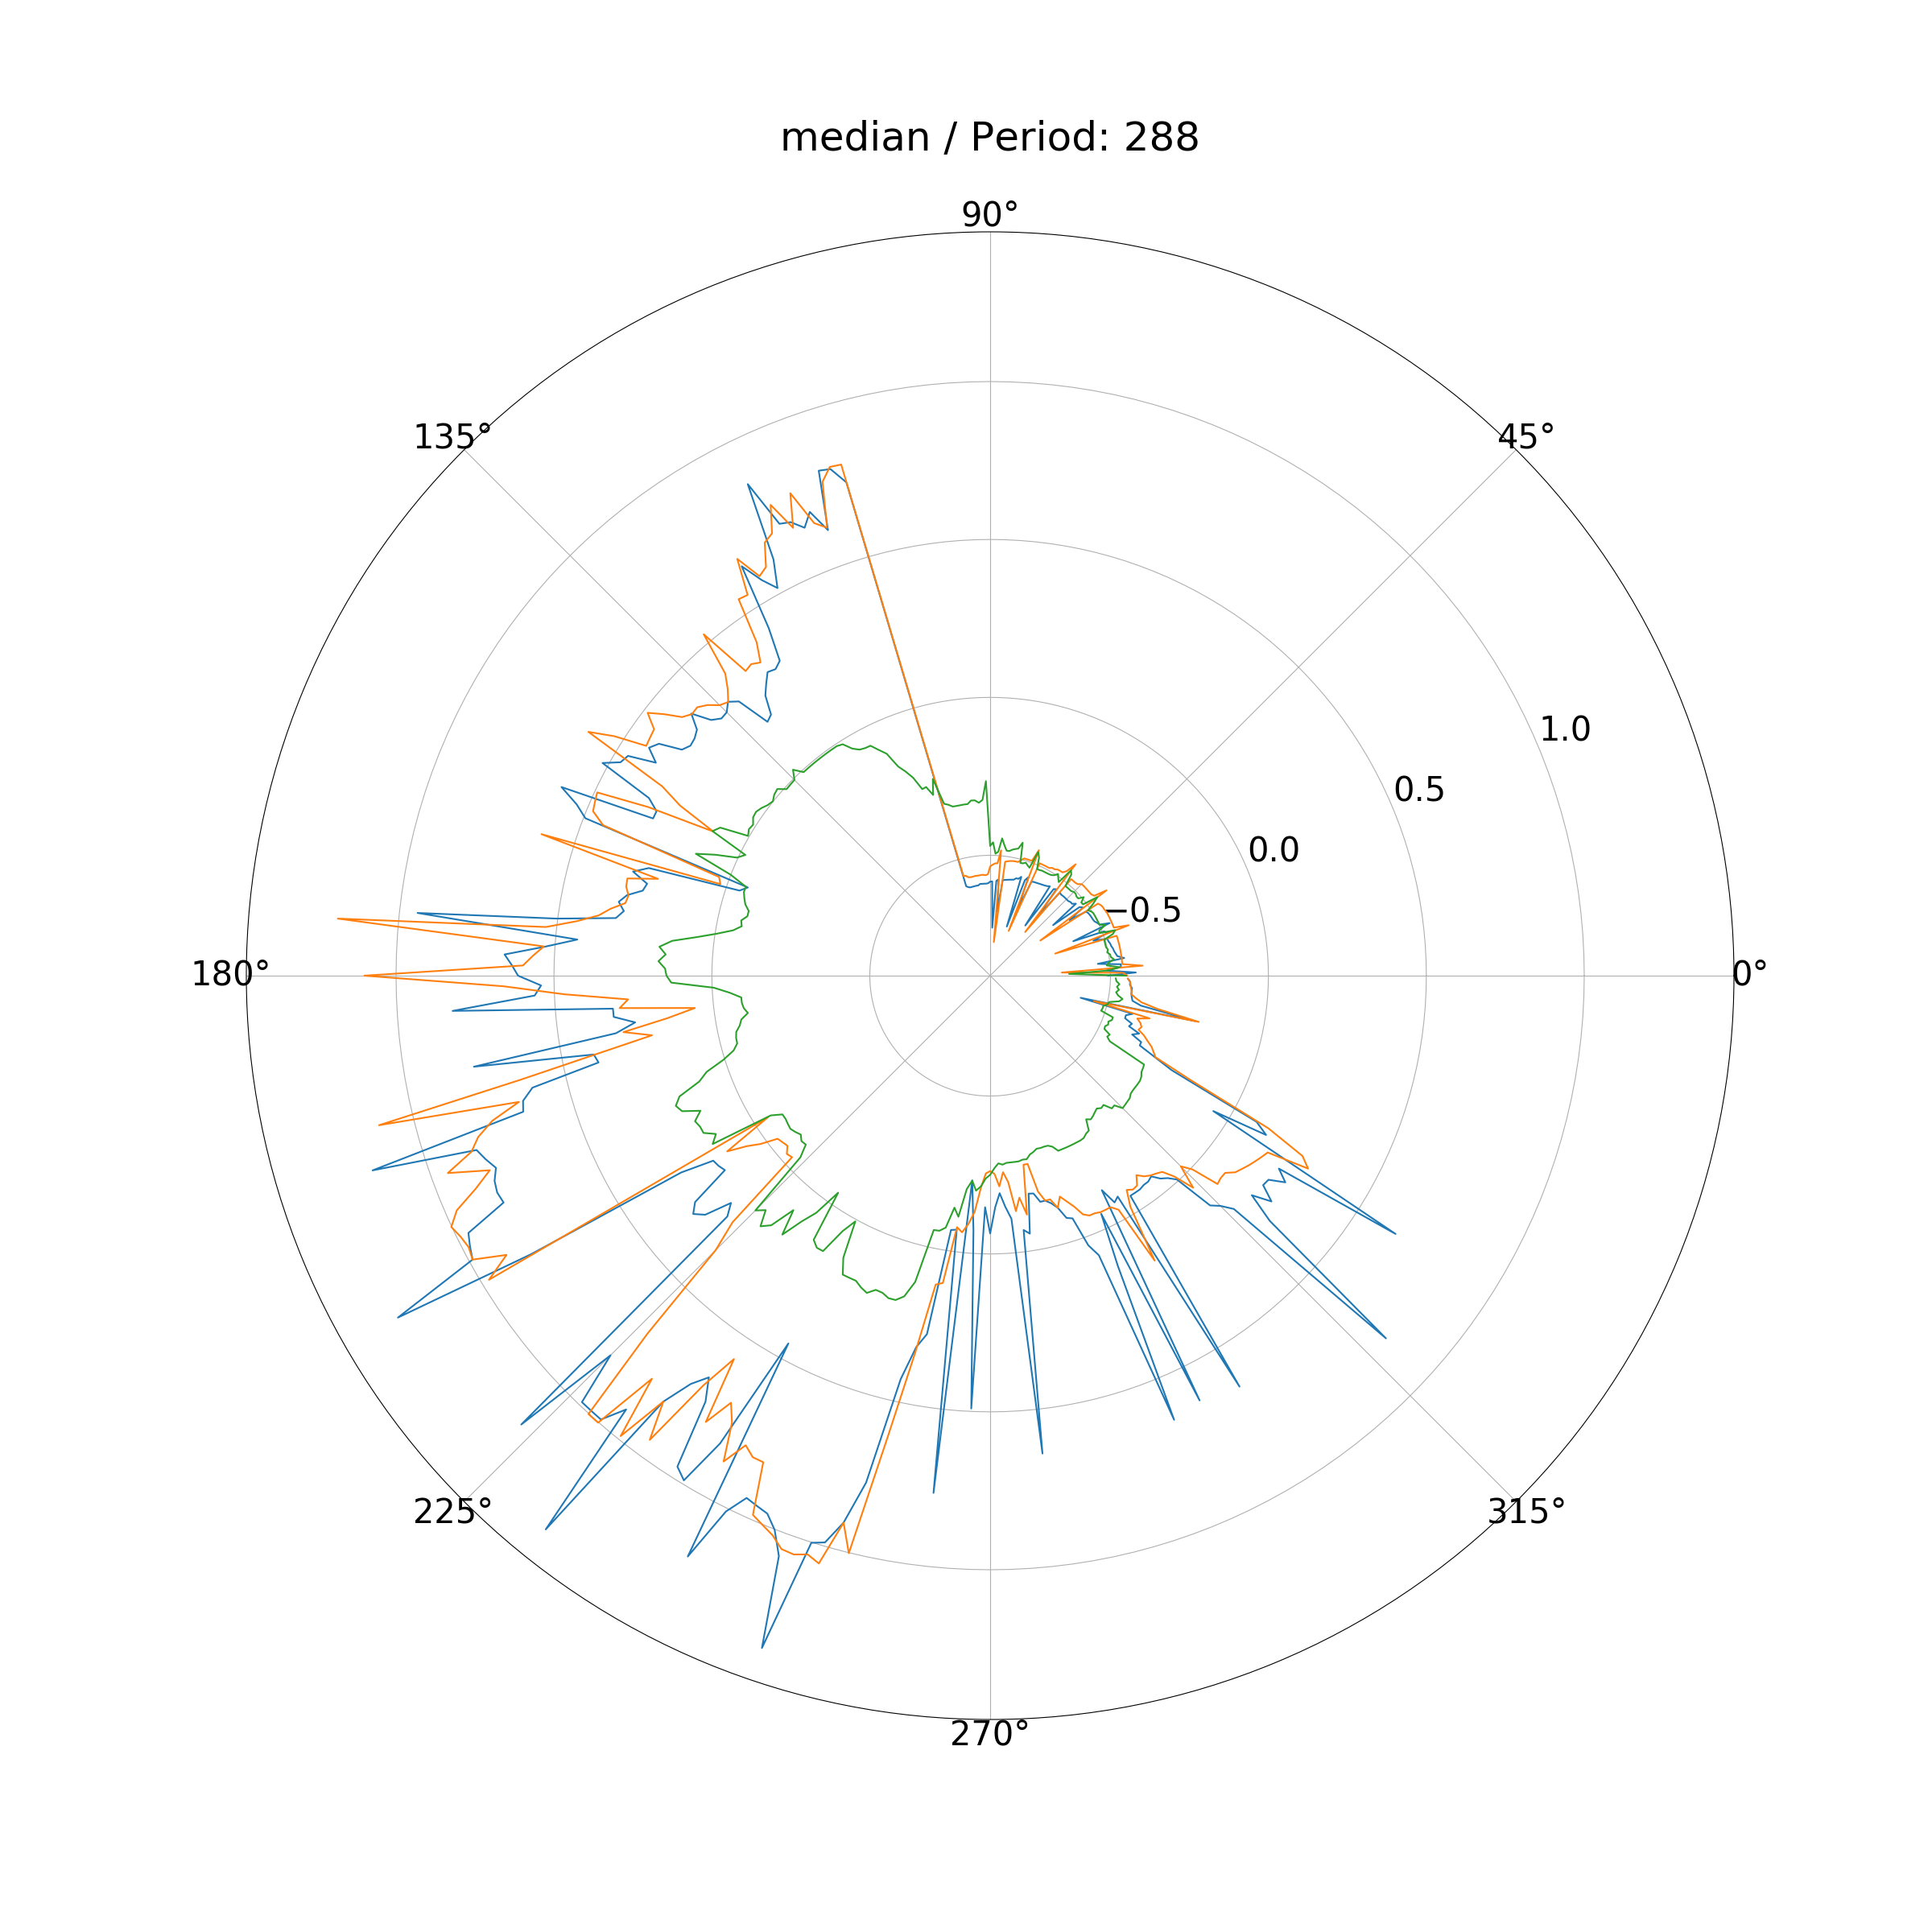
\includegraphics[width=0.3 \linewidth]{figures/third2.png}
                    \\
                    \mbox{(a) Mean} & \mbox{(b) Median} \\
                    
                    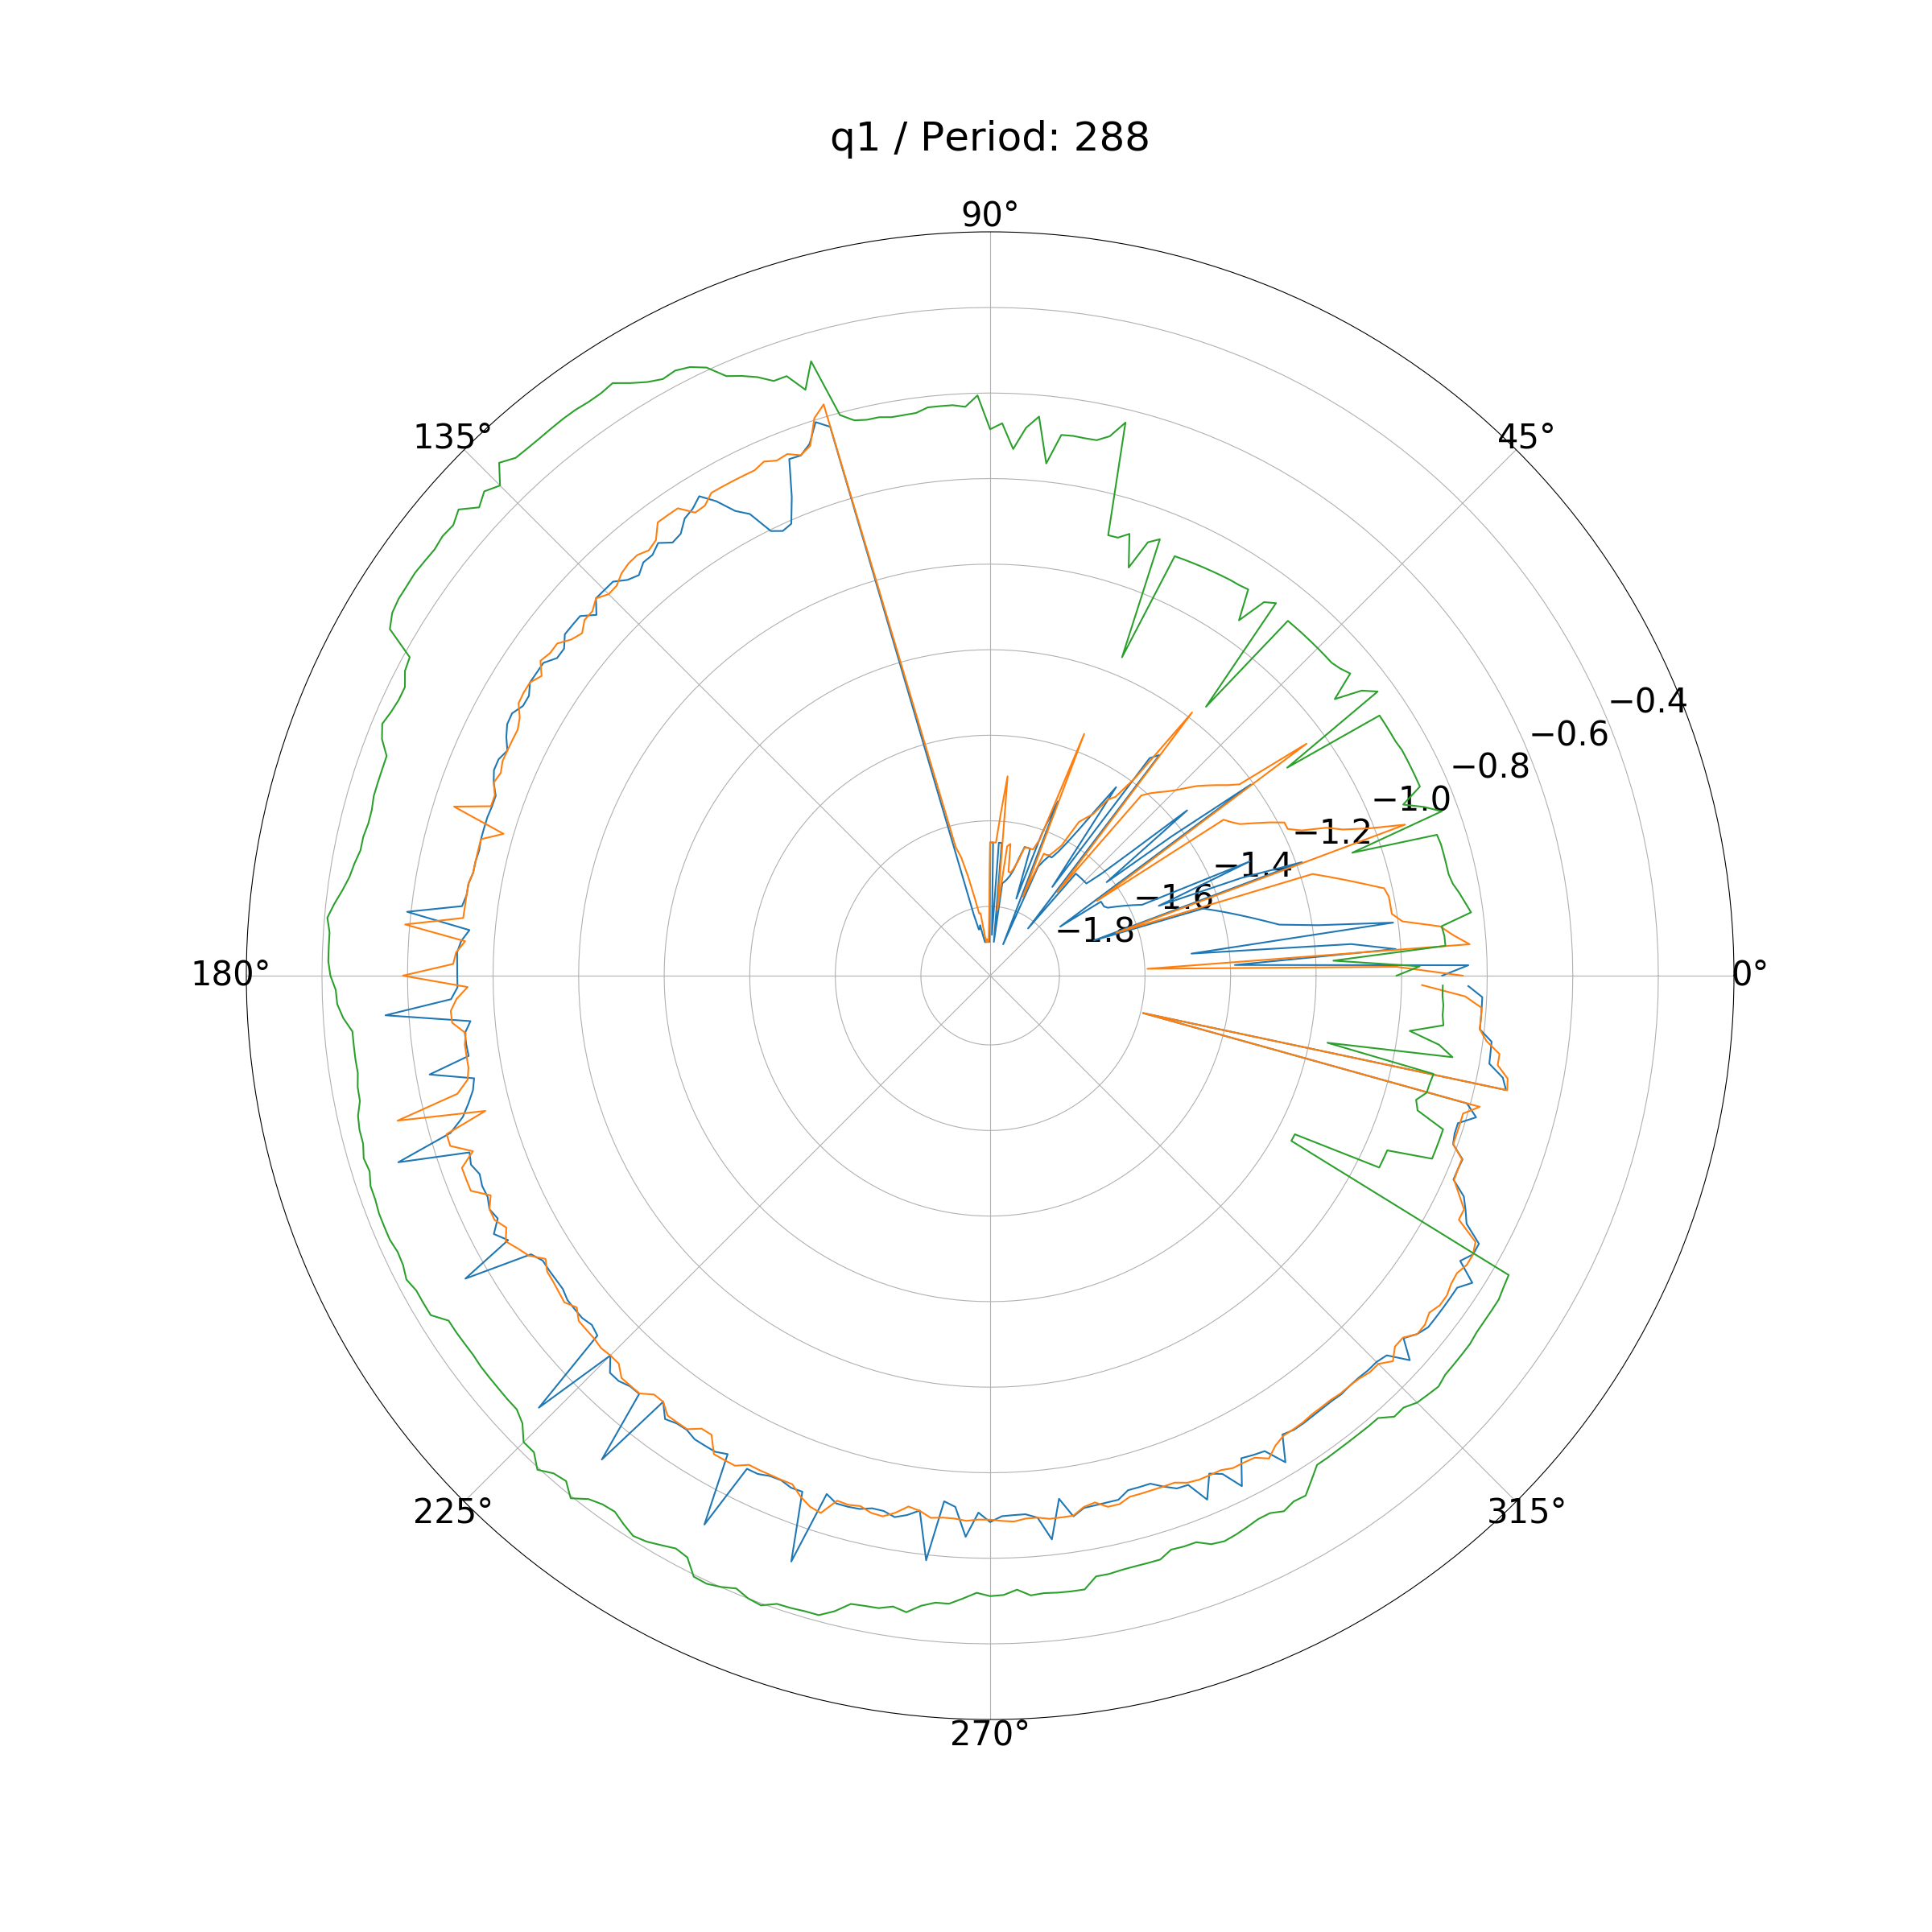
\includegraphics[width=0.3 \linewidth]{figures/third3.png}
                    &
                    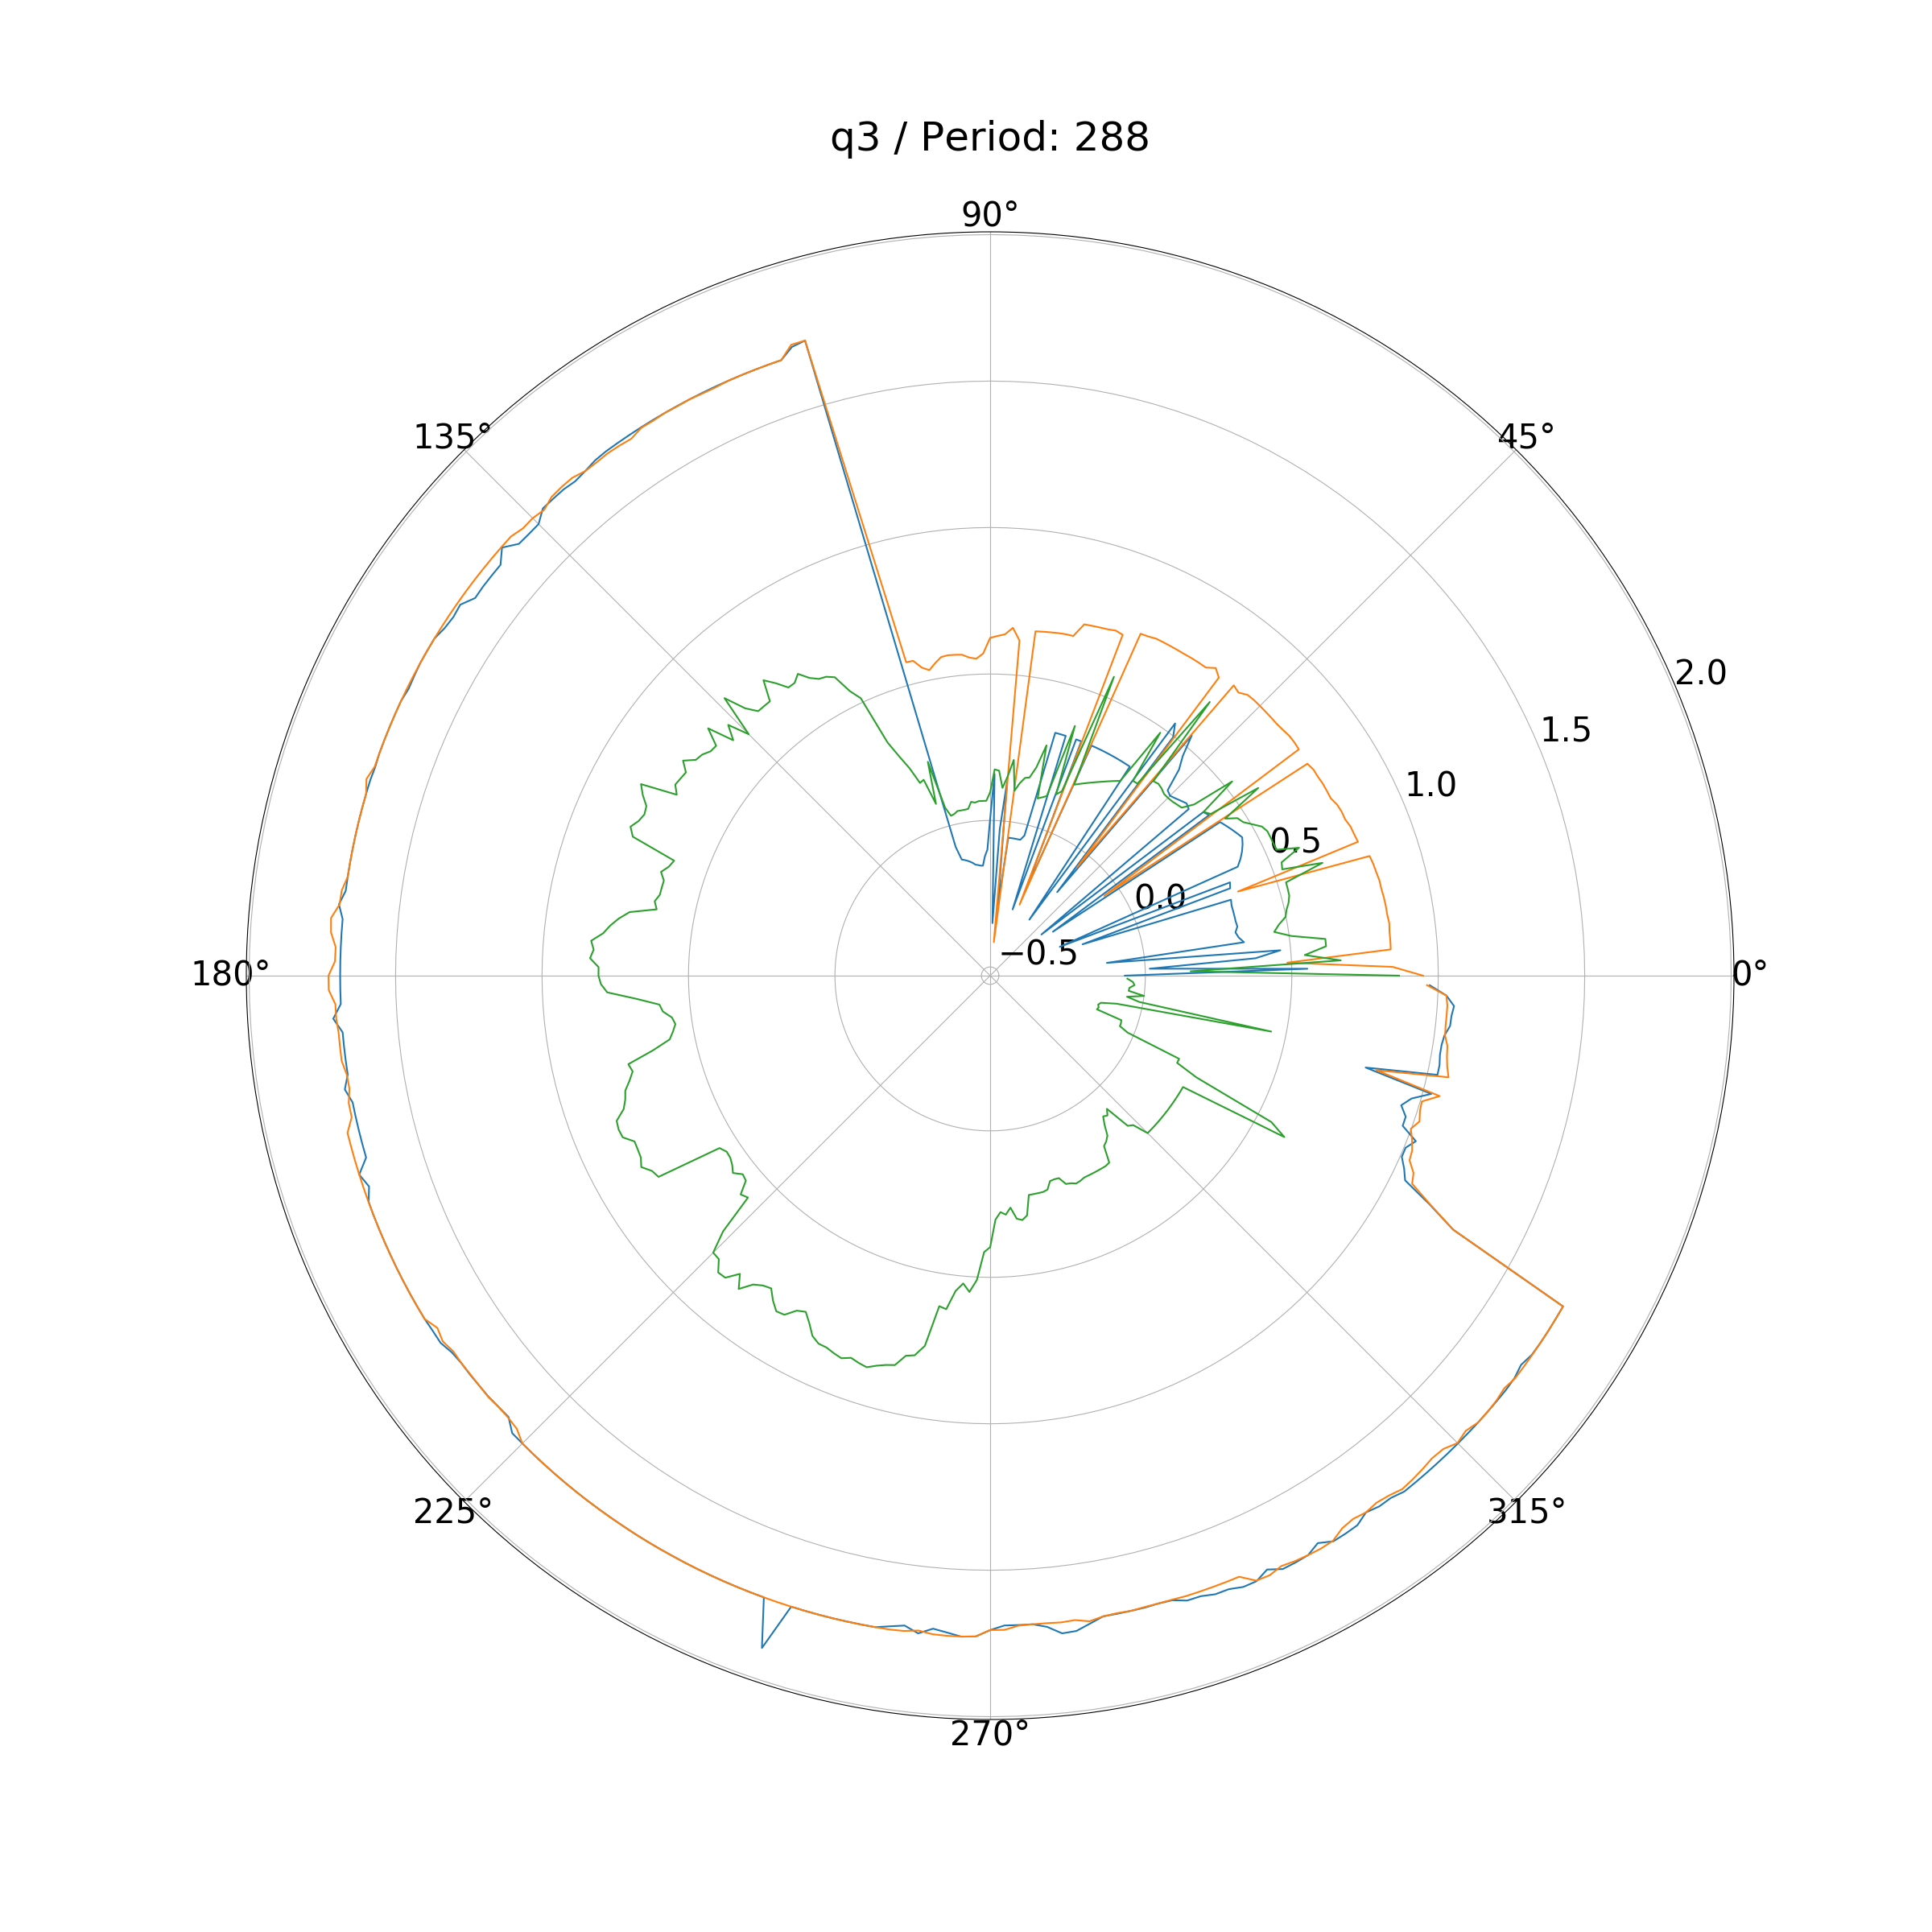
\includegraphics[width=0.3 \linewidth]{figures/third4.png}
                    \\
                    \mbox{(c) q1} & \mbox{(d) q3} \\
                    \end{array}$
                    \caption{Cyclic Plots on Third-quarters}
                    \label{fig:thirdq}
                \end{figure}
            
                In the fourth-quarter, we calculated the under-peak in every columns in general building data. As figure \ref{fig:secondq}, with figure \ref{fig:fourthq}-(a), the distribution of under-peak width is displayed; and, with figure \ref{fig:fourthq}-(b), you can know that where is under-peak in general building data. Moreover, table \ref{tb:fourthq} shows basic statistics value of under-peak width. Amongst the data in figure \ref{fig:fourthq} and table \ref{tb:fourthq}, we can know that the general building data are rapidly decreasing about \textit{16 indices}; in other words, the general building data has under-steeps every \textit{80 minutes}.
                
                \begin{table}[htbp]
                    \centering
                    \caption{Basic Statistics Data with the under-peak in the Fourth-quarter}
                    \label{tb:fourthq}
                    \begin{tabular}{c||c|c|c|c|c|c|c}
                        Item & Minimum & Maximum & Mean & q1 & Median & q3 & Standard Deviation \\ \hline
                        Value & 1.0 & 850.54 & 16.36 & 1.11 & 2.77 & 11.68 & 69.86 \\
                    \end{tabular}
                \end{table}
                
                \begin{figure}[htbp]
                    \centering
                    $\begin{array}{cc}
                        \includegraphics[width=0.4 \linewidth]{figures/fourth1.png}
                        &
                        \includegraphics[width=0.4 \linewidth]{figures/fourth2.png}
                        \\
                        
                        \mbox{(a) Under-peak Width Distribution} & \mbox{(b) Under-peak in Mean Column}
                    \end{array}$
                    \caption{Under-peak in the Fourth-quarter}
                    \label{fig:fourthq}
                \end{figure}
            
            \subsubsection{Interesting Patterns}                                
                According to these fact, we can know followings:
                \begin{enumerate}
                    \item \textit{Thermostat Setpoint} is controlled by floor. Someone can adjust specific zone in floor, but the default value is sets on floor. (Table \ref{tb:rmax})
                    \item Some zone only have \textit{lights} for power consumption. (Table \ref{tb:rmax})
                    \item No \textit{strong} negative correlation exist. (Figure \ref{fig:lowest})
                    \item In the first-quarter, the general building data make a cycle everyday. (Figure \ref{fig:firstq})
                    \item In the second-quarter, the general building data are suddenly increasing about every \textit{75 minutes}. (Table \ref{tb:secondq} and Figure \ref{fig:secondq})
                    \item There are two days which are increasing whole usage of the general building data. (Figure \ref{fig:thirdq})
                    \item  In the fourth-quarter, the general building data are dramatically decreasing about every \textit{80 minutes}. (Table \ref{tb:fourthq} and Figure \ref{fig:fourthq})
                \end{enumerate}
        
        \subsection[Question 3]{Describe up to five notable anomalies or unusual events you see in the data. Prioritize those issue that are most likely to represent a danger or a serious issue for building operations.}
            \label{sec:question3}
            \subsubsection{General Information of Hazium Concentration}
                In the question 2 or section \ref{sec:question2}, we need to find a danger or a serious issue for building data. Hence, we suppose that a danger will be related with Hazium concentration. In other words, if there are some danger in building operation, then the Hazium data will be increased along. 
                
                \begin{figure}[htbp]
                    \centering
                    \includegraphics[width=0.4 \linewidth]{figures/hazium.png}
                    \caption{Hazium Data from Different Data Sources}
                    \label{fig:generalhazium}
                \end{figure}
            
                In the figure \ref{fig:generalhazium}, we can see Hazium concentration of many sources. 

            \subsubsection{Workflow}
                \begin{figure}[htbp]
                    \centering
                    \begin{tikzpicture}[node distance = 2cm, auto]
                    \end{tikzpicture}
                    \caption{Workflow for Question 3}
                    \label{fig:workflow3}
                \end{figure}
            
            \subsubsection{Abnormality in General Building Data}       
                To find patterns which appear in the building data, we should find that normality/abnormality in the building data. However, there are over 400 columns in the general building data; therefore, it is almost impossible to find abnormality column-by-column by human. Hence, we used these four algorithms which are included in scikit-learn: \textit{EllipticEnvelope} \cite{ref:normal1}, \textit{OneClassSVM}, \textit{IsolationForest} \cite{ref:normal2, ref:normal3}, and \textit{LocalOutlierFactor} \cite{ref:normal4}.
                
                \begin{figure}[htbp]
                    \centering
                    $\begin{array}{cc}
                    \includegraphics[width=0.4 \linewidth]{figures/normaltime1.png}
                    &
                    \includegraphics[width=0.4 \linewidth]{figures/normaltime2.png}
                    \\
                    
                    \mbox{(a)} & \mbox{(b)} \\
                    \end{array}$
                    \caption{Abnormality in General Building Data by Timeline}
                    \label{fig:abnormaltime}
                \end{figure}
                
                Moreover, we can display the timeline of abnormality as figure \ref{fig:abnormaltime}. In the figure \ref{fig:abnormaltime}-(a), we can know that which algorithm consider specific time as abnormal events (yellow marked is abnormal); and, in the figure \ref{fig:abnormaltime}-(b), we can realize that how many algorithms consider specific time as abnormal events.
            
            \subsubsection{Score of Classification of Abnormality}
                To decide the best algorithm for find abnormality, we use these five classifier algorithms for scoring: \textit{KNeighbor}, \textit{SVC} \cite{ref:svc1, ref:svc2}, \textit{DecisionTree} \cite{ref:decisiontree1, ref:decisiontree2, ref:decisiontree3}, \textit{RandomForest} \cite{ref:decisiontree3}, and \textit{AdaBoost} \cite{ref:ada1, ref:ada2}. The scores are in table \ref{tb:abnormal}; the highest score is \textit{0.9938} on \textit{LocalOutlier} algorithm. Therefore, we choose \textit{LocalOutlier} algorithm for finding abnormality. Note that the train data and the test data are randomly selected with \( 0.8 : 0.2\) ratio, and the seed is specified for repeated result. 
                
                \begin{table}[htbp]
                    \centering
                    \caption{Scores of Classification of Abnormality}
                    \label{tb:abnormal}
                    \begin{tabular}{c|cccc}
                        & Elliptic & OneClassSVM & IsolationForest & LocalOutlier \\ \hline
                        KNeighbor & 0.995 & 0.991 & 0.929 & 0.988 \\
                        SVC & 0.994 & 0.993 & 0.919 & 0.985 \\
                        DecisionTree & 0.988 & 0.989 & 0.948 & 0.999 \\
                        RandomForest & 0.993 & 0.995 & 0.942 & 0.999 \\
                        AdaBoost & 0.986 & 0.985 & 0.937 & 0.999 \\ \hline
                        Mean & 0.9911 & 0.9906 & 0.9351 & 0.9938 \\
                    \end{tabular}
                \end{table}
            
            \subsubsection{Column for Abnormality}
                Now, we know that when is abnormal in general building data, and the general building data \textit{per se}. Therefore, we can calculate the difference of mean value for each columns in general building data. In other words, we can measure that which column in general building data most differ between normal and abnormal timing.
                
                The distribution of differences between mean values for whole columns of general building data is figure \ref{fig:dmean}; also, the basic statistics values of differences between mean values are in table \ref{tb:dmean}.
                
                \begin{table}[htbp]
                    \centering
                    \caption{Basic Statistics Data with the Differences of Mean Values}
                    \label{tb:dmean}
                    \begin{tabular}{c||c|c|c|c|c|c|c}
                        Item & Minimum & Maximum & Mean & q1 & Median & q3 & Standard Deviation \\ \hline
                        Value & 0.00058 & 1.05075 & 0.159379 & 0.05347 & 0.1097855 & 0.1756 & 0.171869 \\
                    \end{tabular}
                \end{table}
            
                \begin{figure}[htbp]
                    \centering
                    \includegraphics[width=0.4 \linewidth]{figures/meanvalue.png}
                    \caption{Distribution of Differences between Mean Value}
                    \label{fig:dmean}
                \end{figure}
            
            \subsubsection{Danger for Building Operation}
                Figure \ref{fig:heatmap1} display two heatmap about R-values: figure \ref{fig:heatmap1}-(a) is consist with the data which marked as \textit{normal}; and, figure \ref{fig:heatmap1}-(b) contains the data which marked as \textit{abnormal}. However, as shown as figure \ref{fig:heatmap1}, the R-values are not significant; in other words, R-squared values are too small to give confidence for correlation. Therefore, we divided the abnormal data with comparing the general building data and Hazium data directly. As we mentioned herein-above, all of values are standardized, so we can compare two values one-by-one.
                
                \begin{figure}[htbp]
                    \centering
                    $\begin{array}{cc}
                        \includegraphics[width=0.4 \linewidth]{figures/HeatmapNormal.png}
                        &
                        \includegraphics[width=0.4 \linewidth]{figures/HeatmapAbnormal.png}
                        \\
                        \mbox{(a) Normal} & \mbox{(b) Abnormal}
                    \end{array}$
                    \caption{Heatmap of R-values between General Building Data and Hazium Data}
                    \label{fig:heatmap1}
                \end{figure}
            
                Figure \ref{fig:heatmap2} contains two heatmap plot of divided abnormal data. Figure \ref{fig:heatmap2}-(a) is drawn with the data which has higher general building data than Hazium data; and also, figure \ref{fig:heatmap2}-(b) is written with the data which has lower general building data. With comparing figure \ref{fig:heatmap1} and figure \ref{fig:heatmap2}, the R-values in \ref{fig:heatmap2} is bigger than the R-values in \ref{fig:heatmap2}. In other words, in the (General Building Data)--(Hazium Data) plot, the scatter data are aligned near the X-axis and Y-axis. 
            
                \begin{figure}[htbp]
                    \centering
                    $\begin{array}{cc}
                        \includegraphics[width=0.4 \linewidth]{figures/HeatmapHigher.png}
                        &
                        \includegraphics[width=0.4 \linewidth]{figures/HeatmapLower.png}
                        \\
                        
                        \mbox{(a) Higher} & \mbox{(b) Lower} \\
                    \end{array}$
                    \caption{Heatmap of R-values with Higher and Lower General Building Data}
                    \label{fig:heatmap2}
                \end{figure}
            
                With the data in figure \ref{fig:heatmap2}, we can select the column which has the highest sum of R-values. In this data, combination of the column (\textit{F\_2\_Z\_16 SUPPLY INLET Temperature}) and the data set (\textit{f2z2-MC2.csv}) has the highest value. Figure \ref{fig:scatter} is written with this combination. As we mentioned herein-above, many points are along the X-axis or the Y-axis. 
                
                $\therefore$ Hence, if the data (\textit{F\_2\_Z\_16 SUPPLY INLET Temperature}) is decreasing, then the Hazium concentration of Zone 2 on Floor 2 will be increasing; and \textit{vice versa}. Many other combinations exist; but, we only display this combination which has the highest R-values.
            
                \begin{figure}[htbp]
                    \centering
                    \includegraphics[width=0.4 \linewidth]{figures/scatter.png}
                    \caption{Scatter Plot between General Building Data and Hazium Data}
                    \label{fig:scatter}
                \end{figure}
        
        \subsection[Question 4]{Describe up to three observed relationships between the proximity card data and building data elements. If you find a causal relationship, describe your discovered cause and effect, the evidence you found the support it, and your level of confidence in your assessment of the relationship.}
            \label{sec:question4}
            \subsubsection{Frequency of prox Data}
                The general building data has been reported every five minutes; however, prox data is a kind of movement data, so prox data has no cycle pattern at all. Therefore, we should gather and count prox data for comparing with general building data. In this manner, table \ref{tb:freq} and figure \ref{fig:freq} have the distribution information about frequence of prox data. 
            
                \begin{table}[htbp]
                    \centering
                    \caption{Basic Statistics Data with the Frequency of prox Data}
                    \label{tb:freq}
                    \begin{tabular}{c||c|c|c|c|c|c|c}
                        Item & Minimum & Maximum & Mean & q1 & Median & q3 & Standard Deviation \\ \hline
                        Value & 0 & 141 & 8.014 & 0 & 0 & 10 & 15.35 \\
                    \end{tabular}
                \end{table}
            
                \begin{figure}[htbp]
                    \centering
                    \includegraphics[width=0.4 \linewidth]{figures/freq.png}
                    \caption{Distribution with Frequency of prox Data}
                    \label{fig:freq}
                \end{figure}
            
                Moreover, with figure \ref{fig:timeline}, there are some peaks in the prox data. Also, the five peaks in the row, we can have reasonable doubt about weekday and weekend. 
                
                \begin{figure}[htbp]
                    \centering
                    \includegraphics[width=0.4 \linewidth]{figures/daily.png}
                    \caption{Timeline with Frequency of prox Data}
                    \label{fig:timeline}
                \end{figure}
            
                With the reasonable doubt from figure \ref{fig:timeline}, we can draw the cycle plot with daily as figure \ref{fig:dailyprox}. With figure \ref{fig:dailyprox}, we can know what the employees look like such as their attendance time. 
                
                \begin{figure}[htbp]
                    \centering
                    $\begin{array}{ccc}
                        \includegraphics[width=0.3 \linewidth]{figures/dailycycle1.png}
                        &
                        \includegraphics[width=0.3 \linewidth]{figures/dailycycle2.png}
                        &
                        \includegraphics[width=0.3 \linewidth]{figures/dailycycle3.png}
                        \\
                        
                        \mbox{(a) Total data} & \mbox{(b) Fixed data}  & \mbox{(c) Mobile data}
                    \end{array}$
                    \caption{Daily Cycle of prox Data}
                    \label{fig:dailyprox}
                \end{figure}
            
            \subsubsection{Workflow}
                \begin{figure}[htbp]
                    \centering
                    \begin{tikzpicture}[node distance = 2cm, auto]
                    \end{tikzpicture}
                    \caption{Workflow for Question 4}
                    \label{fig:workflow4}
                \end{figure}
            
            \subsubsection{Abnormality of General Building Data and prox Data}
                As question 3 or section \ref{sec:question3}, we ran the abnormality finding algorithms of the merged data amongst the general building data and prox frequency data. Figure \ref{fig:abnormalprox} shows the abnormality of prox data which calculated by four algorithms. 
                
                \begin{figure}[htbp]
                    \centering
                    $\begin{array}{cc}
                        \includegraphics[width=0.4 \linewidth]{figures/abnormalprox1.png}
                        &
                        \includegraphics[width=0.4 \linewidth]{figures/abnormalprox2.png}
                        \\
                        
                        \mbox{(a)} & \mbox{(b)}
                    \end{array}$
                    \caption{Abnormality in prox Data by Timeline}
                    \label{fig:abnormalprox}
                \end{figure}
            
            \subsubsection{Correlation between General Building Data and prox Data}
            
            \subsubsection{Cause and Effect for the Correlation}
    
    \section{Discussion}
    
    \bibliographystyle{ieeetr}
    \bibliography{reference}
\end{document}